\documentclass[smallauthor, chapterhaspagenum, nochapterinheader, pagenuminheader,  bigchapnum,medium2, tocpages, garamond, titleinheader]{jote-book}

\usepackage[dutch]{babel}

\newfloat{bookboxfloat}{th!}{bbxf}

\counterwithout{footnote}{chapter}
\definecolor{orcidlogocol}{HTML}{A6CE39}
\RequirePackage{academicons}
\newcommand{\orcid}[1]{ \href{https://orcid.org/#1}{\textcolor{orcidlogocol}{\kern -0.2em \aiOrcid \kern -0.2em}} }


\newtcolorbox{bookboxf}[1]{
  sharp corners,
  enhanced,
  before skip = {\baselineskip},
  toptitle = {.5\baselineskip},
  bottom = \baselineskip,
  right = \baselineskip,
  colframe = gray!5,
  coltitle = black,
  colback = white,
  colbacktitle = white,
}

\newtcolorbox{bookbox}[1]{
  title = {\textsc{#1}},
  sharp corners,
  enhanced,
  before skip = {\baselineskip},
  toptitle = {.5\baselineskip},
  bottom = \baselineskip,
  right = \baselineskip,
  colframe = gray!5,
  titlerule=0pt,
  coltitle = black,
  colback = gray!5,
  colbacktitle = gray!5,
  breakable,
}

\newtcolorbox{bookboxnotitle}{
  sharp corners,
  enhanced,
  before skip = {\baselineskip},
  toptitle = {.5\baselineskip},
  bottom = \baselineskip,
  right = \baselineskip,
  colframe = gray!5,
  coltitle = black,
  colback = white,
  colbacktitle = white,
  breakable,
}

\newtcolorbox[auto counter]{briefcolorbox}{
  enhanced ,
  breakable,
  sharp corners,
  frame hidden,
  pad at break*=1mm,
  colback=white,
  title={\centering\textbf{\textit{\Large Chapter in Brief\vspace*{2\baselineskip}}}},
  fonttitle=\bfseries,
  colframe=gray!5,
  coltitle=gray!50!black,
  subtitle style={bottomrule=.5pt,
      toprule=0pt,
      colback=gray!5,
      coltext=gray!70!black},
  width=.9\linewidth
}


\booktitle{De Universiteit in Transitie}
\booksubtitle{}
\bookauthor{Henk Kummeling\orcid{0009-0001-0052-3990}, Manon Kluijtmans\orcid{0000-0001-6601-7639}, Frank Miedema\orcid{0000-0002-8063-5799}}
\pagecolor{white}
\bookkeywords{Open Science\index{open science}}
\bookpublisher{Publishers of Trial and Error}
\booksubject{Open}
\bookyear{2023}
\bookcopyrightholder{Manon Kluijtmans, Henk Kummeling, Frank Miedema}
\bookcopyright{\noindent Dit boek en al het materiaal dat het bevat zijn gelicentieerd onder het Creative Commons 4.0 Internationaal (CC BY-NC 4.0) licentie, wat betekent dat je vrij bent om het werk te kopiëren, verspreiden, en remixen, zolang je de maker van het werk \href{https://creativecommons.org/licenses/by-nc/4.0/deed.nl}{vermeldt}, een link naar de licentie plaatst en aangeeft of het werk veranderd is.
  Voor meer informatie, zie \\\mbox{\url{https://www.creativecommons.org/licenses/by/4.0/legalcode}}.}

\booklicenseurl{https://www.creativecommons.org/licenses/by/4.0/legalcode}
\bookcontactemail{publishers@trialanderror.org}
\bookcontacturl{https://trialanderror.org}
\bookisbn{}
\bookurl{https://uu.trialanderror.org/book}
\bookdoi{}
\bookpublisherlogo{logo.png}
\bookpublisherlocation{Utrecht, Nederland}
\othercredits{\noindent Design and Typesetting by \href{https://tefkah.com}{Thomas F. K. Jorna}\\
\noindent Cover design by \href{https://morlumbroso.com}{Mor Lumbroso}\\
  \noindent Coordination by \href{https://www.linkedin.com/in/violet-zagt/}{Violet S. Zagt}\\
  
  In samenwerking met Utrecht Universiteit \hspace*{10em} \raisebox{-2em}{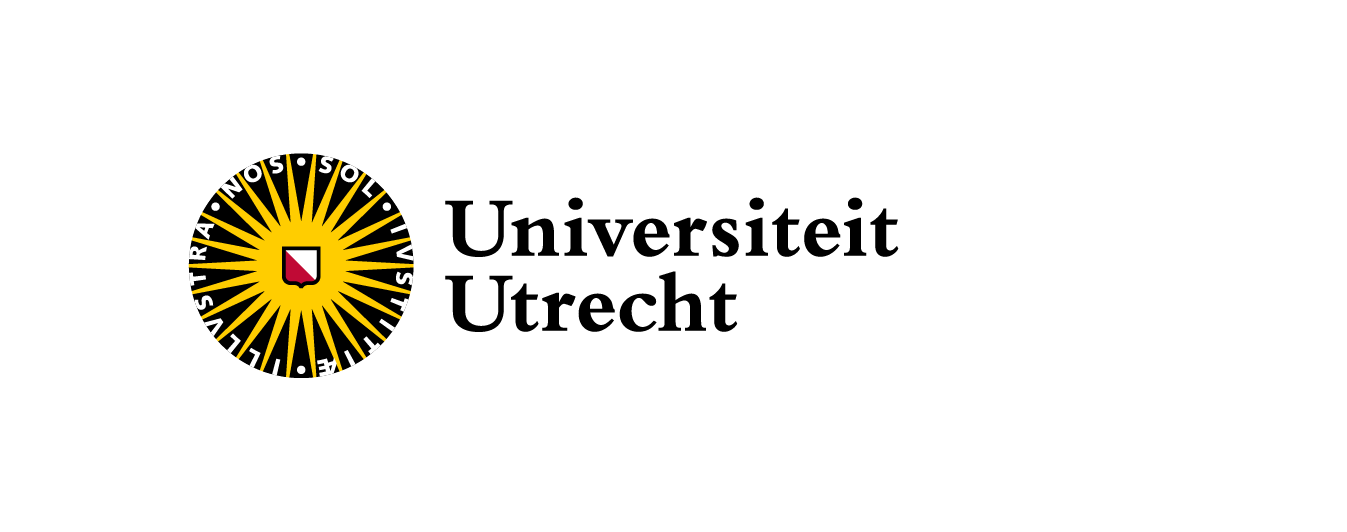
\includegraphics[height=5em]{uu.png}}\\}

\bookversion{Preprint Versie}

\NewEnviron{references}{
  {
      \RaggedRight
      \small
      \setlength{\leftskip}{1em}
      \setlength{\parindent}{-1em}
      \noindent\BODY
    }
}

\makeindex


\begin{document}
	
\frontmatter
\pagestyle{empty}
\begin{center}
  \vfill
  \emph{De Universiteit in Transitie}
  \vfill
\end{center}
\clearpage
\clearpage
\copyrightpage
\clearpage
\titlepage

\cleartorecto
\pagestyle{empty}
\tableofcontents



\cleartoverso
\mainmatter

\pagestyle{ruled}
\addcontentsline{toc}{chapter}{ Proloog }

	\chapter*{ Proloog }

	\nochapterinheader



	Dat universiteiten vitale, veerkrachtige instituties zijn met een groot aanpassingsvermogen is tijdens de coronapandemie nog maar weer eens gebleken. In een paar dagen tijd ging vrijwel al het onderwijs online en kon ook veel van het onderzoek worden voortgezet door opzet of methode te veranderen, onderdelen te temporiseren, labtijden te flexibiliseren etc. Tijdens de pandemie bleek ook weer eens overduidelijk wat de enorme betekenis is van fundamenteel én toegepast onderzoek is voor de samenleving, zeker als dit onderzoek plaatsvindt in een internationale context; met een ontzagwekkende snelheid konden vaccins, medicijnen en behandelmethoden worden ontwikkeld.



	Gelijktijdig werd ook zichtbaar dat er in delen van de samenleving grote scepsis bestaat ten aanzien de resultaten van wetenschappelijk onderzoek, zeker als op basis daarvan wordt ingegrepen in vrijheden en rechten van burgers, zoals bij tal van overheidsmaatregelen ter bestrijding van de pandemie, maar ook die in het kader van de aanpak van de klimaatcrisis. Op de sociale media worden in een rap tempo alternatieve waarheden ontwikkeld, die wetenschap reduceert tot ‘ook maar een mening'.



	In de achterliggende jaren werden universiteiten nog met andere zorgen geconfronteerd. Academische vrijheid\index{academische vrijheid} en institutionele autonomie staan op veel plaatsen onder druk, ook in landen waar deze vrijwel onaantastbaar leken zoals in de Verenigde Staten van Amerika. Prestatie- en werkdruk, gecombineerd met gebrekkige financiering\index{financiering} doen universiteiten in hun voegen kraken. In het bijzonder de prestatiedruk heeft zelfs tot een fundamentele vragen geleid: welke prestaties zijn eigenlijk de moeite waard? En: voor wie willen we eigenlijk prestaties leveren? Vragen die in essentie gaan over de legitimiteit van de universiteit.



	Als vanzelf stelt zich dan de vraag hoe de universiteit zich gaat ontwikkelen. Nog interessanter was voor ons de vraag: hoe hopen we dat de universiteit zich gaat ontwikkelen? Misschien zelfs wel: wat is de ideale universiteit? Dat zou al snel kunnen leiden tot futuristische dagdromerij, waar alleen maar tijdelijk plezier aan valt te beleven. De opdracht die wij ons gesteld hebben, is om na te denken over een wenkend perspectief dat een stevige basis heeft in de realiteit, in de ontwikkelingen die we om ons heen zien.







	Natuurlijk wordt er voortdurend nagedacht over de manier waarop de universiteit zich ontwikkelt. Dat heeft in de recente jaren ook interessante publicaties opgeleverd, zoals die van de voormalige rector magnificus van de UU, Bert van der Zwaan, onder de wat omineuze titel: ‘Haalt de universiteit 2040?'\footnote{Van der Zwaan, \emph{Haalt de universiteit 2040?}} Daarin behandelt hij vooral het stelsel van hoger onderwijs in Europees in internationaal perspectief. Daarnaast was er ook nog de publicatie van Floris Cohen, verleidelijk getiteld: ‘De ideale universiteit', waarin hij zich grotendeels baserend op een aantal funderende beginselen, zette aan het ontwerp van een nieuwe universiteit, die op onderdelen toch verrassend veel lijkt op de universiteit die we in het (verre) verleden kenden.\footnote{Cohen, \emph{De Ideale Universiteit}\emph{.}} Deze en vele andere publicaties hebben onze gedachten gescherpt én ons tot de conclusie gebracht dat het de moeite waard zou kunnen zijn om nog eens verder na te denken over de toekomst van de universiteit vanuit de inhoudelijke ontwikkeling van de kerntaken van de universiteit, te weten onderwijs, onderzoek en maatschappelijke impact. Die kerntaken ontwikkelen zich in de context van dé grote culturele verandering in de academische wereld in de huidige tijd, die naar \emph{Open }\emph{Science}. In wezen gaat het er bij deze verandering om dat de universiteit zich meer wil verankeren in de samenleving door de grote maatschappelijk uitdagingen op lokaal, regionaal en globaal niveau meer centraal te stellen in onderwijs en onderzoek, maar ook door meer aan de samenleving terug te geven.\footnote{Uitvoeriger over de ontwikkeling van \emph{Open }\emph{Science} in Hoofdstuk 2.} Hoe is het onderwijs en onderzoek zich, mede in die context aan het ontwikkelen?



	De universiteit, dat zijn de mensen, en daarom is het ook van groot belang om te bezien hoe de universitaire gemeenschap\index{gemeenschap} zich ontwikkelt en idealiter zich zou kunnen ontwikkelen. Vanzelfsprekend moet dan ook het oog gericht zijn op de organisatie van de universiteit. Hiermee zijn ook al de hoofdthema's van dit boek gegeven: onderwijs, onderzoek, samenleving, gemeenschap\index{gemeenschap} en organisatie. Het geheel wordt gecompleteerd door een korte historische schets en een epiloog waarin de voornaamste conclusies en wenkende perspectieven bij elkaar worden gebracht.



	Onze ambitie reikt, op bescheiden wijze, verder dan het louter beschrijven van wat we menen waar te nemen; we willen ook aangeven welke vervolgontwikkelingen we verwachten en wenselijk vinden. Soms geven we ook aan welke stappen nodig zijn om bepaalde idealen te kunnen realiseren. En uiteraard zijn het daarmee ook aanzetten voor discussie.



	Er zijn er velen die relevant zijn voor het bepalen van de toekomst van de universiteit. Allereerst de leden van de universitaire gemeenschap\index{gemeenschap} zelf, studenten en medewerkers. Daarnaast zijn er natuurlijk ook de politici, beleids- en opiniemakers. En daarbuiten zijn er tal van andere actoren die van betekenis zijn, of op zijn minst geïnteresseerd zijn in het functioneren van de universiteit en op beslissende momenten, bijvoorbeeld bij verkiezingen, invloed kunnen uitoefenen.



	Met dat brede publiek voor ogen hebben we geprobeerd een zo toegankelijk mogelijk boek te schrijven, met veel ruimte voor uitleg en voorbeelden. Aangezien wij alle drie verbonden zijn aan de Universiteit Utrecht, en we rijkelijk geput hebben uit onze eigen ervaringen, zal het niet verbazen dat nogal wat voorbeelden afkomstig zijn uit Utrechtse praktijken. Daarmee is het geen ‘Utrechtse visie' geworden, laat staat dat we de Universiteit Utrecht ten voorbeeld willen stellen. Integendeel, volgens ons is datgene wat we behandelen op zijn minst in meer of mindere mate relevant voor alle Nederlandse universiteiten. Hoogwaardig onderzoek is per definitie internationaal, en daarmee is de universitaire wereld per definitie ook een internationale wereld, waarbinnen de laatste jaren de Europese Unie in toenemende mate van belang is, zowel beleidsmatig als voor onderzoeks- en onderwijsfinanciering. Die internationale, en in het bijzonder Europese context, zal in dit boek dan ook vaak aan bod komen.



	Vanwege die internationale context is het van belang om aan te geven wat in dit boek onder universiteit verstaan. We zullen het vooral hebben over wat internationaal wel aangeduid wordt als ‘\emph{research }\emph{universities}\emph{'}. Dat zijn niet, zoals wel eens wordt gedacht, universiteiten die prioriteit geven aan onderzoek. Het gaat om instellingen van hoger onderwijs die onderzoek als basis van hun activiteiten hebben, en waarbij het onderzoek dus ook de basis vormt voor het onderwijs. Dit in tegenstelling tot hoger onderwijsinstellingen waarbij dit niet primair het geval is. In internationaal verband worden deze vaak aangeduid als ‘\emph{university}\emph{ of }\emph{applied}\emph{ }\emph{sciences}\emph{'}. Het Nederlandse Hoger Beroeps Onderwijs\index{hoger beroeps onderwijs (HBO)} past in de laatste categorie. In de praktijk is het onderscheid tussen deze beide types instelling niet zo scherp te maken; (toegepast) onderzoek krijgt ook steeds meer aandacht in de hoek van de \emph{universities}\emph{ of }\emph{applied}\emph{ }\emph{sciences}\emph{.} Het is dan ook begrijpelijk dat, zeker binnen de EU, in toenemende mate wordt uitgegaan van gelijkwaardigheid van beide types instelling. Er blijft echter ook een waardevol en te koesteren verschil tussen de instellingen die gericht zijn op opleiden van mensen die nieuwe hoogwaardige kennis genereren, en instellingen die zich richten op het opleiden van mensen die in staat zijn hoogwaardige kennis toe te passen (en daar ook onderzoek naar doen).\footnote{Zie ook het position paper VSNU-VH doorontwikkeling binair stelsel 2019 (\href{https://www.universiteitenvannederland.nl/files/documenten/Publicaties/Position_paper_VH_VSNU_binair_stelsel_september_2019.pdf}{https://www.universiteitenvannederland.nl/files/documenten/Publicaties/Position\_paper\_VH\_VSNU\_binair\_stelsel\_september\_2019.pdf}).} Dit boek gaat vooral over dat wat er gebeurt aan het eerstgenoemde type instelling. Veel van wat wij te melden hebben zal echter ook relevant zijn voor HBO-instellingen, zeker op het gebied van onderwijs. Maar ons past hier ook bescheidenheid; we kennen het HBO\index{hoger beroeps onderwijs (HBO)} niet van binnenuit.



	Velen hebben ons geïnspireerd bij dit project. Allereerst tal van nationale en internationale auteurs. Maar zeker zo waardevol waren de inzichten die naaste collega's en studenten met ons wilden delen. Toen we met het onderwerp aan de slag gingen hebben we een drietal bijeenkomsten belegd met studenten en collega's van wie we zeker wisten dat ze affiniteit, kennis en ervaring hadden op de onderwerpen die we in het bijzonder breder wilden bespreken: onderwijs, public engagement\index{public engagement} en de universitaire gemeenschap\index{gemeenschap}. Aan onze uitnodiging om deel te nemen aan van wat wij ‘\emph{expert}\emph{ }\emph{meetings}' genoemd hebben, werd massaal gehoor gegeven. De input, maar ook de belangstelling was zeer stimulerend. Achteraf kregen wij te horen dat het wel jammer was dat niet nog meer mensen aanwezig hadden kunnen zijn en dat de bijeenkomsten zo beperkt in aantal waren. Een mooiere manier om te merken dat een onderwerp waar je bezig bent ‘leeft' is er eigenlijk niet. Wij danken alle deelnemers aan deze ‘expertmeetings', en ook degenen die er niet bij konden zijn en ons schriftelijk van inbreng voorzagen. Hun namen zijn te vinden in een bijlage.



	Degene die we zeker ook willen bedanken is Claire Stalenhoef, ten tijde van het schrijven student aan de UU, in de Legal Research Master. Zij heeft voor de verzameling en bundeling van onderzoeksmateriaal gezorgd en ook de coördinatie van de expertmeetings was in haar handen. Zij gaf waardevolle inhoudelijke feedback\index{feedback, feed-up, feedforward} en zorgde er ook voor dat we ook het studentperspectief voor ogen hielden. Datzelfde geldt ook voor Manar el Amrani, die halverwege het project de verantwoordelijkheden van haar overnam. Claire en Manar ‘organiseerden' het auteursteam, hetgeen gelet op de bijzondere agenda's van de schrijvers bepaald een uitdaging was. Met schijnbaar onuitputtelijke kwaliteit en opgewektheid hebben zij hun klussen geklaard.



	Als auteurs hebben we het werk verdeeld. Manon Kluijtmans heeft de primaire verantwoordelijkheid gehad voor de hoofdstukken over onderwijs en gemeenschap\index{gemeenschap}. Frank Miedema heeft vooral de hoofdstukken over de transitie naar \emph{Open }\emph{Science} en die naar de interactie met de samenleving voor zijn rekening genomen. Henk Kummeling gaf de voorzet voor de andere stukken. Het geheel is echter een resultaat van een indringende samenwerking, waarvoor we gezamenlijk de verantwoordelijkheid nemen. In dat verband willen we ook zeker Maarten Post bedanken, die de rol van kritische meelezer vervulde. Hij heeft vooral gelet op de toegankelijkheid van de teksten, en hij heeft ook er ook voor gezorgd dat de hoofdstukken taalkundig wat zijn gestroomlijnd, waarmee overigens niet kon worden voorkomen dat de hand van een bepaalde auteur zichtbaar bleef. De hoofdstukken vertonen uiteraard samenhang, maar we hebben er ook voor willen zorgen dat ze afzonderlijk leesbaar en begrijpelijk zijn.



	Geheel in lijn met de \emph{Open }\emph{Science} gedachte, maken we ons werk nu eerst digitaal beschikbaar voor iedereen. We zijn heel benieuwd naar reacties, suggesties en voorbeelden. Op basis daarvan gaan wij waarschijnlijk over een half jaar aan de slag met een nieuwe versie van de tekst, die ook op papier zal verschijnen.



	\vspace*{\baselineskip}

	\noindent Henk Kummeling, Manon Kluijtmans, Frank Miedema

	\vspace*{\baselineskip}

	\noindent April 2023





	\chapter{Beknopte ontwikkelingsgeschiedenis van de universiteit }



	\section{In den beginne…}



	De universiteit kennen we als instituut al heel lang. Meestal wordt 1088, met de vestiging van de universiteit van Bologna, als geboortejaar gezien.\footnote{Ter voorkoming van misverstanden: dat was niet het geboortejaar van de wetenschap. Die kwam veel eerder op, ook in andere delen van de wereld zoals in China, Egypte, Babylonië en natuurlijk ook Griekenland. Zie Cohen, \emph{Modern }\emph{Science}\emph{,}\emph{ }3-4.} Maar de bestaansgeschiedenis voert nog verder terug, namelijk naar 859, het jaar waarin de Al-Qarawiyyin Universiteit te Fez werd opgericht.\footnote{Hoque et al., ‘World's Oldest University', 24-4; Verbrugge, ‘De universiteit'.} Sindsdien heeft de institutie een buitengewoon succesvolle opmars gemaakt in Europa en de rest van de wereld.\footnote{De World Higher Education Base (WHED), van de International Association of Universities en UNESCO\index{UNESCO}, bevat gegevens van meer dan 20.000 universiteiten (waarvan ca 5.000 in Europa) en dat aantal blijft maar stijgen. Zie www.whed.net} Het bestaansrecht van het instituut universiteit als zodanig is al die eeuwen nooit omstreden geweest. Dat geldt wel voor het idee van de universiteit. Waartoe dient de universiteit eigenlijk? Het antwoord op die vraag is al die tijd voortdurend aan discussie en verandering onderhevig geweest, tot op de dag van vandaag aan toe.\footnote{Zie ook de treffende titel van de essaybundel onder redactie van Verbrugge, \emph{Waartoe is de Universiteit op Aarde}\emph{?}}



	Aanvankelijk verzorgden universiteiten in Europa vooral een opleiding in de theologie ten behoeve van de katholieke kerk onder patronage van de wereldlijke vorst.\footnote{Van der Zwaan, \emph{Haalt de Universiteit }\emph{2040?,} 32; Verbrugge, ‘De Universiteit', 208.} Dat de instelling van een universiteit vaak ook een politieke achtergrond had en ook nadrukkelijk in de context werd gezien van landsbestuur en identiteit blijkt bijvoorbeeld uit de vestiging van de universiteit van Leiden in 1575. Die werd door Willem van Oranje nadrukkelijk neergezet als een alternatief voor andere, sterk katholiek georiënteerde, universiteiten. De nieuwe universiteit had onder andere tot doel om weerbare en scherpzinnige burgers op te leiden, ‘opdat de vijand nooit meer zo gemakkelijk zijn verzengende tirannie en onderdrukking van de godsdienst, of de vrijheden van het land met geweld dan wel listigheid in gang zou kunnen zetten'. Om dat mogelijk te maken was niet alleen opleiding ‘in de juiste kennis van God', maar ook in ‘de vrije kunsten en wetenschappen' nodig.\footnote{Zie van Stipriaan, \emph{De Zwijger}, 441, waaraan ook bovenstaande citaat zijn ontleend.} Het inzicht dat de samenleving maar ook het centrale en decentrale bestuur\index{bestuur} behoefte had aan andere dan theologische kennis, was ook al eerder bij de bestaande universiteiten doorgedrongen. Er werden ook al eerder beroepsopleidingen aangeboden voor artsen en juristen, of wat breder: bestuurders.\footnote{Verbrugge, ‘De Universiteit', 209; Langereis, \emph{Erasmus}\emph{, }87.} En ook toen al ging het bij deze opleidingen niet louter om onderwijs dat gericht was op een specifiek beroep. Opvallend was dat veel Middeleeuwse universiteiten een vergelijkbaar basiscurriculum kenden voor alle opleidingen. Daarbij ging het om algemene vorming en taalbeheersing, waarbij kennis van het Latijn, spreken en schrijven met overtuigingskracht en logica centraal stonden.\footnote{van Bommel, ‘De teloorgang', 175; Verbrugge, ‘De Universiteit', 209; Cohen, \emph{Modern }\emph{Science}, 81} Met name de opkomst en brede omarming van de Aristotelische logica, waarin autonoom systematisch denken centraal staat, zorgde ervoor dat universiteiten steeds zelfstandiger, losser van het kerkelijk en wereldlijk gezag, functioneerden.\footnote{Cohen, \emph{Modern }\emph{Science}, 79.} In de op de middeleeuwen volgende Renaissance werd deze ontwikkeling verder versterkt. Met het teruggrijpen op de klassieke oudheid en de aandacht voor de beste literatuur uit die tijd, werd de morele dimensie van de opleidingen verlegd. Nog steeds stond vorming tot deugdzame mensen centraal, maar dan deugdzaam niet zozeer in de ogen van God, maar vooral in termen van geschiktheid om verantwoordelijke posities in de samenleving, het openbare leven te kunnen vervullen.\footnote{van Bommel, ‘De teloorgang', 176.} De opkomst van het humanisme, waarin de waarde van de mens, het kritische denken en bewijs centraal staan en theologische dogma's met argusogen worden bekeken, heeft hierbij een enorme betekenis gehad.



	\section{Verlichting}



	In de 18\textsuperscript{e} eeuw vond tijdens De Verlichting een fundamentele verandering plaats; de rede werd dominant voor het denken. De wetenschap, en daarmee ook de universiteiten maakten zich definitief los van religieuze en deels ook wereldlijke normstellingen door zich geheel te richten op objectiviteit. Er kwamen twee uitgangspunten centraal te staan, die ook in de huidige tijd nog als kernwaarden voor de universiteit gelden, namelijk onafhankelijkheid en neutraliteit.\footnote{Van der Zwaan, \emph{Haalt de Universiteit }\emph{2040?}, 34.} Het was ook de tijd van de opkomst van de burgercultuur; niet langer de kerk en de adel waren bepalend, maar ‘gewone' burgers. Organisatie en handelen van de staat werden voorwerp van analyse en kritiek. Er kwam veel meer aandacht voor volk, geschiedenis, eigen taal en ideologie en dat had ook praktische gevolgen voor de universiteit en rol van universitair geschoolden in de samenleving. In de woorden van Verbrugge werden het meer broedplaatsen voor journalisten en revolutionairen.\footnote{Verbrugge, ‘De Universiteit', 209.}



	\section{Bildung met onderzoek}



	Dat brengt ons bij een volgende mijlpaal in ontwikkelingsgeschiedenis van universiteiten, die van de ‘\emph{Bildung\index{bildung}}\emph{'}\emph{. }Over het idee van \emph{Bildung\index{bildung}} is en wordt ontzaglijk veel geschreven vanuit verschillende (romantische) invalshoeken. Wij volgen hier de lijn die al eerder door Francot en De Vries is uitgezet.\footnote{Francot et al., ‘Adieu von Humboldt\index{humboldt}?', 74-77.} Zij wijzen op het werk van Horlacher waarin \emph{Bildung\index{bildung}} wordt gezien als een holistisch concept gericht op het realiseren van een betere samenleving, zowel economisch, moreel als politiek.\footnote{Horlacher, ‘\emph{Bildung\index{bildung}}', 409-26.} Universitair onderwijs wordt als uitermate belangrijk gezien voor de verwezenlijking van dit ideaal. Het ideaal van \emph{Bildung\index{bildung}} is voor altijd verbonden met Wilhelm von Humboldt\index{humboldt}, wetenschapper en staatsman, die stelde dat de belangrijkste functie van de universiteit is het samenvoegen van studenten in een gemeenschap\index{gemeenschap} die gewijd is aan wetenschap en het veiligstellen van hun totale vrijheid om kennis en inzichten uit te wisselen en zichzelf te ontplooien in een omgeving doordrenkt van wetenschap, niet onderworpen aan dwang of beperkt door directe doeleinden.\footnote{Francot et al., ‘Adieu von Humboldt\index{humboldt}?', 75-76.}



	Von Humboldt\index{humboldt} kreeg de gelegenheid om zijn ideeën als minister van onderwijs van Pruisen te realiseren. Tot op de dag van vandaag geldt op de oprichting van de Universiteit van Berlijn (tegenwoordig bekend als Humboldt\index{humboldt} Universität) in 1810 als een van zijn belangrijkste erfstukken. Maar zijn gedachtengoed is ook nog steeds levend. Een paar elementen daaruit verdienen bijzondere aandacht. Allereerst het idee, dat eigenlijk al uit de Verlichting stamt, dat het onderwijs vrij moet zijn van staatsinmenging. Belangrijk is ook dat het onderwijs gericht moet zijn op individuele, innerlijke zelfontwikkeling. Die individualiteit moet ontwikkeld worden door de uitwisseling van ervaringen met anderen. Sociale banden en interactie zijn dus in het onderwijs cruciaal. Tenslotte kan niet genoeg benadrukt worden, omdat dit in discussies over het ideale universitaire onderwijs vaak vergeten wordt, dat volgens Von Humboldt\index{humboldt} de universiteit juist door de eenheid van onderwijs en onderzoek een optimaal klimaat voor \emph{Bildung\index{bildung}} zou moeten garanderen.\footnote{Francot et al., ‘Adieu von Humboldt\index{humboldt}?', 76.}



	In die institutionalisering van de combinatie van onderwijs en onderzoek in de universiteit, waarbij de universiteit zich ook nog eens ontwikkelde van doorgever van bestaande kennis, naar een instituut waarin nieuwe kennis werd verworven, moet de blijvende betekenis van Von Humboldt\index{humboldt} worden gezocht. In die combinatie van onderwijs en onderzoek zag hij het onderscheidende kenmerk van de universiteit.\footnote{Van der Zwaan, \emph{Haalt de Universiteit }\emph{2040?,} 35.} Deze essentiële combinatie in het denken van Von Humboldt\index{humboldt} werd in latere jaren soms uit het oog verloren, zoals hierna zal blijken.



	\section{Onderzoek zonder Bildung?}



	\emph{Bildung\index{bildung}} wordt tegenwoordig vaak vooral gezien als een welhaast romantisch ideaal voor het onderwijs. Daarmee wordt vaak vergeten dat onderzoek een essentiële component is van het Bildungsideaal van Von Humboldt\index{humboldt}. Er wordt dan ook wel gezegd dat de oprichting van de universiteit van Berlijn vooral de opkomst van de ‘onderzoeksuniversiteit' markeert. Kennisuitbreiding werd de voornaamste missie van de universiteit. ‘De primaire taak van de universiteit werd te voorzien in de financiële, logistieke en andere middelen die de productie van nieuwe kennis faciliteren. Onderzoeks-\emph{seminars}, \emph{graduate}\emph{ schools}, gespecialiseerde onderzoeksinstituten en laboratoria zagen vanaf de late negentiende eeuw aan vrijwel alle Europese en Amerikaanse universiteiten het licht', aldus Van Bommel.\footnote{van Bommel, ‘De teloorgang', 178.} Dit is een ontwikkeling die zich in de twintigste eeuw heeft voortgezet. De kennisuitbreiding vond in toenemende plaats in de natuurwetenschappen, de biomedische hoek, landbouw en techniek. Dat werd door overheden krachtig gestimuleerd, zeker na de Tweede Wereldoorlog.\footnote{Frank Miedema, \emph{Open }\emph{Science}\emph{, }1.}



	Volgens Van Bommel heeft niets het denken over academische vorming radicaler veranderd dan deze herdefinitie van de universiteit als onderzoeksinstituut:

	\begin{quote}
		\itshape

		‘De academische status van moderne universiteitsdocenten berust niet op hun vermogen studenten intellectueel en moreel te vormen, maar op de “vernieuwingen” of “ontdekkingen” die ze op hun naam hebben staan'.\footnote{van Bommel, ‘De teloorgang', 178.}
	\end{quote}

	Hoewel op de scherpte van Van Bommel nog wel wat is af te dingen is\footnote{Het belang van onderwijs als primaire taak van de universiteit wordt de laatste jaren, inclusief de betekenis die dit moet hebben voor academische carrières, (weer) steeds breder onderschreven. En dat was op sommige plaatsen al het geval voor de opkomst van \emph{Open }\emph{Science}. Zie verder Hoofdstuk 3.}, is het onmiskenbaar zo dat de opdracht tot algemene vorming aan universiteiten steeds minder aandacht heeft gekregen, en dat had ook consequenties voor de status en de rol van de sociale -- en vooral de geesteswetenschappen, die juist in het kader van de algemene vorming in het verleden zo'n dominante rol hadden vervuld aan de universiteit. Het statusverlies van deze wetenschapsgebieden werd nog verder versterkt doordat zij minder evidente of spectaculaire ontdekkingen op hun naam konden schrijven, en dat had vervolgens weer negatieve gevolgen voor hun financiering\index{financiering}. Een vraagstuk waar we later nog op terug komen.



	Naast het vraagstuk van de verhouding tussen de verschillende wetenschapsgebieden, ontstond in toenemende mate het vraagstuk van de verhouding tussen onderwijs en onderzoek als kerntaken van de universiteit. Onderwijs werd een last, ook omdat universitaire carrières vooral werden gemaakt op basis van onderzoeksprestaties. Die ontwikkeling heeft bijgedragen aan een existentiële crisis in de universitaire wereld. Die crisis kent echter meerdere facetten, die in samenhang aandacht behoeven.



	\section{De aanloop naar fundamentele vragen voor de universiteit}



	De universiteit is in de jaren zestig van de vorige eeuw wezenlijk van karakter en betekenis veranderd doordat de poorten opengingen voor studenten die, anders dan voorheen, niet afkomstig waren uit de ‘gegoede burgerij'. Eindelijk konden intelligente studenten uit alle lagen van de bevolking profiteren van de beste opleidingen, die ook nog eens toegang gaven tot de beste, althans hoogst betaalde, banen in de samenleving. Het gevolg was een massale toestroom van studenten. Dat had een relatief kortstondig en een langdurig effect. Bij dat eerste moet vooral gedacht worden aan een toenemende aandacht voor maatschappelijke problemen, de nationale politiek en de toestand in de wereld. Dat leidde tot onder andere demonstraties, bezettingen, protestacties en eisen tot aanpassing van curricula, het stopzetten van contacten met universiteiten in landen met een dubieuze reputatie op het gebied van de mensenrechten.\footnote{Zie voor een recente reflectie Kennedy, ‘Back to the Sixties?'. } Met de opkomst van het neoliberalisme in de jaren tachtig werd dit type idealisme minder beeldbepalend. Wat bleef was de vraag hoe een uitbundig gegroeide universiteit, met daarin groepen met andere en nieuwe ambities, te besturen. De universiteit werd voor die tijd gekenmerkt door hoogleraren-zelfbestuur, daarin geholpen door wat professionele bestuurders in deeltijd. Professionalisering en democratisering van het universiteitsbestuur waren noodzakelijk, maar dit blijft tot aan de dag van vandaag een lastige combinatie.\footnote{Zie verder Hoofdstuk 6, Paragraaf 2.}



	De toestroom van studenten leidde ook tot het optuigen van een omvangrijk ondersteunend apparaat. Deze bureaucratie\index{bureaucratie} bracht vanzelfsprekend regels, procedures en verantwoordingsplichten met zich. Een ontwikkeling die nog verder werd versterkt doordat de noodzakelijke financiering\index{financiering} van de universiteiten achterbleef bij de toestroom van studenten en nog sterker gedacht moest worden in termen van efficiency. Sterker nog, vanaf de jaren tachtig van de vorige eeuw werden er door de Nederlandse overheid diverse bezuinigingsoperaties doorgevoerd. De studieduur werd beperkt en onder druk van de overheid werden opleidingen geschrapt.\footnote{Het is eerst is de resultaten van de wet Twee Fasen Structuur en aan het schrappen van opleidingen lag de nota ‘Selectieve krimp en groei' ten grondslag, Meer hierover in Hoofdstuk 6, Paragraaf 2.} Uiteindelijk werd door de Nederlandse overheid alleen nog maar de nominale studieduur gefinancierd, waardoor iedere ‘langstudeerder' een belasting werd voor universiteiten, niet alleen voor de financiële middelen, maar door de verdunning van de middelen ook een bedreiging voor de kwaliteit van het onderwijs. De druk op de financiering\index{financiering} van het onderzoek werd vergroot doordat onderzoekmiddelen uit de eerste geldstroom werden weggehaald en in een aparte organisatie werden gezet, aanvankelijk geheten de Organisatie voor Zuiver Wetenschappelijk onderzoek, vanaf 1988 getiteld: de Nederlandse Organisatie voor Wetenschappelijk Onderzoek\index{nederlandse organisatie voor wetenschappelijk onderzoek (NWO)} (NWO\index{nederlandse organisatie voor wetenschappelijk onderzoek (NWO)}). Vervolgens konden dan onderzoekers in competitie onder door NWO\index{nederlandse organisatie voor wetenschappelijk onderzoek (NWO)} gestelde condities weer onderzoeksmiddelen naar binnenhalen.



	Deze ontwikkelingen hebben, zeker ook in Nederland, grote gevolgen gehad voor het interne functioneren van universiteiten.\fbox{ }De niet-toereikende overheidsfinanciering\index{overheidsfinanciering} dwong tot nadenken over efficiencyvoordelen en dat leidde weer tot schaalvergroting en centralisatie én verdergaande bureaucratisering.\footnote{Van der Zwaan, \emph{Haalt de Universiteit }\emph{2040?,} 61. } En dat leidde ook weer tot vragen over welke ruimte er nog was voor de academische onafhankelijkheid en vrijheid en de professionele autonomie\index{professionele autonomie } van de afzonderlijke medewerkers.



	De krapte in de financiering\index{financiering} leidde ook tot een speurtocht naar andere bronnen, zoals het bedrijfsleven. In de jaren tachtig van de vorige eeuw kwam in Nederland ook het concept van de ‘ondernemende universiteit' op. Met als vertrekpunt de erkenning van het praktische belang van de wetenschap voor de samenleving werd betoogd dat de universiteit meer met wetenschappelijke kennis moest ondernemen. Al snel werd dit door de critici gezien als een knieval voor het bedrijfsleven.\footnote{Zie de boeiende rede van Alexander Rinnooy Kan bij de opening van het academisch jaar van de universiteit Twente op 5 september 2011, getiteld: ‘Naar een ondernemende universiteit: u nadert uw bestemming?' Als geestelijk vader van de term ‘ondernemende universiteit' noemt hij de voormalige rector van de UT, prof. Harry van den Kroonenberg, die in een artikel uit 1985 de term voor het eerste gebruikte.} Gegeven de context van de zwaar bezuinigende kabinetten-Lubbers was dat natuurlijk niet zo verwonderlijk. Terwijl aandacht voor meer maatschappelijke relevantie in beginsel helemaal niet verkeerd is, waarover later meer, kleurde de context van de financieringsvraag van meet af de speurtocht naar externe financiering\index{financiering} als bedreiging voor de academische waarden van de universiteit in negatieve zin.



	Op gebied van onderzoek is het zoeken naar externe financiering\index{financiering} heel dominant geworden. Dat geldt in zijn algemeenheid, inclusief overheidsfinanciering\index{overheidsfinanciering} en financiering\index{financiering} vanuit het bedrijfsleven. Maar het geldt in het bijzonder voor de financiering\index{financiering} in de vorm van de beurzen van NWO\index{nederlandse organisatie voor wetenschappelijk onderzoek (NWO)} en European Research Council (ERC), die voor het individuele carrièreperspectief heel dominant zijn geworden - en als prestigieus worden ervaren. De toekenning van dergelijke financiering\index{financiering} is vaak thematisch bepaald, met als gevolg dat bepaalde onderzoekers, thema's en disciplines minder kans op financiering\index{financiering} hebben. Dat heeft tot een scheefgroei in de financiering\index{financiering} van de wetenschapsgebieden geleid, waarbij wereldwijd, maar ook in Nederland, de medische, technische en natuurwetenschappen verreweg het grootste deel van de middelen binnenhalen, met bijvoorbeeld als gevolg dat in Nederland 70\% van de wetenschappelijke staf werkzaam is in deze domeinen.\footnote{Miedema, \emph{Open }\emph{Science}, 7.}\footnote{Van der Zwaan, ‘Transformative power', 233.}



	De speurtocht naar externe, waaronder private, financiering\index{financiering} heeft de universiteit wereldwijd tot een uiterst competitieve omgeving gemaakt. Mede onder invloed van het in de jaren tachtig opgekomen neoliberalisme en het gedachtengoed van New Public Management\index{new public management}, waarin getracht werd kwaliteit te sturen door ze vooral in meetbare eenheden te vervatten, werden bepaalde ‘\emph{metrics\index{metrics}}', zoals de Hirsch-index\footnote{Een discipline-afhankelijk indicator, die beoogt de wetenschappelijke impact van iemands publicaties te meten aan hand van het aantal citaties van een artikel. }, dominante maatstaven voor de toekenning van onderzoeksmiddelen.\footnote{Dorsman, \emph{Het universitaire bedrijf}; voor meer details, zie Lorenz, ‘Feiten Fiksen', 77 e.v.}\textsuperscript{,}\footnote{Zie ook Hoofdstuk 2.} Dit alles heeft geleid tot een bepaalde publicatie- en beoordelingscultuur, die niet alleen de ruimte voor het zetten van eigen onderzoeksagenda's beperkte, maar die ook een academische apenrots creëerde; degenen met de meeste en de hoogste prijzen zaten bovenaan en werden ook gezien als de leiders wier voorbeeld moest worden gevolgd. Dat alles heeft ook binnen het onderzoekdomein bijgedragen aan gevoel van verlies van autonomie, verhoging van de werkdruk, maar soms ook aan gevoelens van onveiligheid. Als oorzaak wordt nadrukkelijk ook de leiderschapscultuur aangewezen.\footnote{Naezer et al., \emph{Harassment}\emph{ in Dutch }\emph{Academia}\emph{.} Zie ook het Koninklijke Nederlandse Akademie van Wetenschappen, \emph{Sociale}\emph{ Veiligheid}, waarin de organisatiestructuur en de daarbinnen bestaande machtsverschillen als belangrijke veroorzakers van sociale onveiligheid worden gezien.} In veel wetenschapsgebieden, maar in het bijzonder weer in het medische, technische en natuurwetenschappelijke domein, werd de voornaamste drijfveer voor wetenschappers om zo snel mogelijk een eigen onderzoekgroep te kunnen starten en deze zo succesvol mogelijk te maken in termen van aantallen publicaties, financiële middelen en mensen. Dat doet iets met de met de onderlinge verhoudingen tussen mensen. De universiteiten werden meer gekenmerkt door een cultuur waarin wetenschappelijke status en leeftijd dominant werden voor de besluitvormingsprocessen. Sommigen zeggen ook wel dat universiteiten zich in dat kader van een democratie naar een gerontocratie ontwikkelden, waarin vooral aandacht is voor gevestigde belangen met bijgevolg serieuze risico's voor vernieuwing.\footnote{Miedema, \emph{Open }\emph{Science}, 11.}



	Het verschil in externe financiële prikkels en verantwoordingsregimes heeft er mede toe geleid dat het logisch leek om onderwijs en onderzoek ook organisatorisch volstrekt te separeren binnen de universiteit, waarmee een van de idealen van Von Humboldt\index{humboldt} werd ondergraven, de koppeling van onderzoek en onderwijs vanuit de gedachte dat vorming vooral plaatsvindt door het verwerven van nieuwe kennis. Deze organisatorische scheiding heeft grote gevolgen gehad, op zijn minst in het universitaire personeelsbeleid en de onderlinge verhoudingen tussen de medewerkers. Omdat carrières vooral werden gemaakt langs de lijn van de onderzoeksprestaties, werd onderwijs voor velen een ‘last' waarvoor je je als het maar enigszins kon moest ‘uitkopen'. Chargerend werd het onderwijs lange tijd het werk voor de ‘jongste bedienden', die op basis van tijdelijke contracten, zonder onderzoekstijd, de bulk van het werk voor hun rekening namen. Dat dit tot grote ontevredenheid onder docenten zou leiden was te voorspellen, als ook dat dit gevolgen zou hebben voor de kwaliteit van het wetenschappelijke onderwijs.



	Een ontwikkeling die onmiskenbaar ook grote gevolgen heeft gehad voor universiteit is die van de internationalisering\index{internationalisering}. In zekere zin keert de universiteit daarmee terug naar haar wortels, want bij aanvang waren de universiteiten al internationaal, althans Europees, enorm verbonden, met veel onderling verkeer van studenten en medewerkers, geholpen door het feit dat er een gemeenschappelijke taal was, het Latijn. In de negentiende eeuw werden universiteiten nationalistischer met veel aandacht voor eigen geschiedenis en taal.\footnote{Verbrugge, ‘De Universiteit', 210.} Daar is pas de laatste decennia verandering in gekomen, onder andere omdat de Europese Unie ter bevordering van de Europese eenheid de uitwisseling van studenten enorm ging stimuleren, onder andere via de zogeheten ERASMUS-programma's.\footnote{En met TEMPUS (‘\emph{Trans-European }\emph{Mobility}\emph{ }\emph{Scheme}\emph{ }\emph{for}\emph{ University Studies}') reikte uitwisselingsambitie zelf ver buiten Europa. European Commission, ‘Trans-European Mobility for University Studies (TEMPUS)', laatst aangepast 30 mei 1990. https://cordis.europa.eu/article/id/31-transeuropean-mobility-for-university-studies-tempus. } Veel belangrijker is echter dat (weer) werd onderkend dat onderzoek per definitie universeel is, en dat de kwaliteit en de ontwikkeling daarvan enorm gebaat is bij internationale contacten en samenwerking. Dat geldt zelfs voor disciplines die ogenschijnlijk vooral een nationaal referentiekader hebben, zoals de rechtswetenschap of taalwetenschappen. Ook daar bedriegt de schijn. Veel van het onderzoek dat daarin plaatsvindt heeft een internationale context en een internationale betekenis.



	Deze ‘internationalisering\index{internationalisering}' heeft positieve gevolgen gehad voor de kwaliteit van het onderwijs en onderzoek. In veel vakgebieden draagt een ‘\emph{international}\emph{ classroom}\emph{'} enorm bij aan begrip en vorming van studenten.\footnote{Sawir, ‘Internationalisation of Higher Education Curriculum\index{curriculum}', 359. } In het onderzoek zijn de kwaliteitseffecten van internationalisering\index{internationalisering} nog minder omstreden. Wel blijft een discussiepunt dat de internationalisering\index{internationalisering} er niet toe mag leiden dat er alleen internationaal wordt gepubliceerd, en dat er voldoende ruimte blijft voor onderzoek dat specifiek aandacht heeft voor nationale, regionale of lokale vraagstukken.\footnote{Wilkinson, ‘English-Medium Instruction', 324. }



	De internationalisering\index{internationalisering} heeft ook minder positieve effecten. De extra toestroom van studenten zet een nog grotere druk op de onderwijsorganisatie, die nog eens wordt versterkt doordat studenten uit de EU onder dezelfde (financiële) voorwaarden als Nederlandse studenten mogen deelnemen aan het onderwijs. Alleen voor de niet-EU studenten (of beter: niet EER-studenten) mogen hogere tarieven in rekening worden gebracht.\footnote{Voor het bredere financiële en economische perspectief zie Bolhaar et al., ‘\emph{Economische Effecten van Internationalisering\index{internationalisering}}\emph{'.}} In onderzoek heeft de internationalisering\index{internationalisering} de onderlinge competitie nog verder versterkt. Internationale samenwerkingen tussen universiteiten werden vooral ingegeven door succes in die competitie, gemeten aan de hand al eerder besproken \emph{metrics\index{metrics}}. Als gevolg daarvan zien we vooral veel officiële samenwerkingen tussen ‘\emph{high-}\emph{ranked}\emph{'}\emph{ }universiteiten van westerse snit. Diepgaande samenwerkingen met universiteiten uit zich ontwikkelende landen zijn zeldzaam, en dat is des te merkwaardiger omdat universiteiten in hun doelstelling vaak hebben staan dat ze willen bijdragen aan het vinden van oplossingen voor de ‘\emph{grand }\emph{challenges}\emph{'}, de grote maatschappelijke nationale, maar ook wereldwijde problemen.\footnote{Leebron, ‘The Global and the Local', 180-181.}



	Dat laatste raakt de fundamentele rol en maatschappelijke legitimatie\index{legitimatie} van de universiteit. Met een beroep op de Verlichtingsidealen van onafhankelijke en waardenvrij wetenschap is vanuit universiteiten vooral betoogd: laat ons met rust en dan doen we wel de goede dingen. Die claim is door diverse oorzaken problematisch gebleken. Allereerst door de wetenschap zelf. Door de fixatie op \emph{metrics\index{metrics}}, de wens en noodzaak tot het scoren in ‘\emph{high }\emph{ranked}\emph{ }\emph{journals}\emph{'}\emph{, }zijn wetenschappers veel meer gericht geraakt op zichzelf in plaats op de noden van de samenleving. Plastisch gezegd: het is ‘\emph{Science}\emph{ }\emph{for}\emph{ }\emph{Scientists}', in plaats van ‘\emph{Science}\emph{ }\emph{for}\emph{ Society}' geworden.\footnote{Hierover wordt in Hoofdstuk 2, Tekstbox 2 - 3 meer over uitgeweid.Zie voor meer info o.a.: Owen et al., ‘Responsible Research and Innovation', 117-126. } Maar het voert te ver om de universiteiten daar alleen de schuld van de te geven. Overheden en andere externe financiers hebben ook een belangrijke bijdrage geleverd aan de ontstane problematiek. Door de sterke fixatie op (spectaculaire) ‘ontdekkingen' en economische effecten\footnote{Zie bijvoorbeeld het zogenaamde topsectoren beleid vanaf 2015, dat beoogde publiek-private samenwerkingsverbanden tussen bedrijfsleven, departementen en kennisinstellingen te bevorderen. Onderdeel daarvan is, aldus de minister van Economische Zaken, die verantwoordelijk is voor dit beleid, dat ‘publieke kennisinstellingen -- naast hun publieke taken [worden] gestimuleerd een deel van de onderzoeksmiddelen in te zetten op thema's die voor het bedrijfsleven relevant zijn'. Zie de Kamerbrief van Wiebes, ‘\emph{Missiegedreven Innovatiebeleid}, 1. }, is er een universiteit ontstaan waarin de medische, technische en natuurwetenschappen dominant zijn geworden, en dat terwijl er voor de analyse en oplossing van grote maatschappelijke vraagstukken, zoals armoede, ongelijkheid, voeding en gezondheid, coherentie, functioneren van de democratie, opgroeien van de jeugd, duurzaamheid, klimaatverandering \emph{etc}., vooral ook andere wetenschapsgebieden noodzakelijk zijn, met name die uit de sociale en geesteswetenschappen.



	De hiervoor gepresenteerde cocktail van vraagstukken heeft ertoe geleid dat universiteit in een crisissfeer is beland, zeker aan het begin van de 21\textsuperscript{e} eeuw. Er dienden zich existentiële vraagstukken aan. Zijn we niet te zeer gericht geraakt op onderzoek, ten koste van onze opdracht in onderwijs? Heeft de hang naar efficiency, met de daarmee gepaard gaande regels, procedures en verantwoordingplichten, niet de noodzakelijke autonomie aangetast? Is er niet te veel aandacht gekomen voor economisch/financieel waardeerbare en meetbare activiteiten? Anders gezegd, ook in samenhang met de vorige vraag, is de ‘economisering' van de universiteit niet te veel doorgeslagen? En de meest fundamentele vraag van alle is: doen we nog wel de goede dingen, in het licht van onze maatschappelijke rol en verantwoordelijkheid?



	\section{De toekomst: Open Science }



	Deze crisissfeer heeft velen tot nadenken aangezet. Bijzonder is dat het vooral een Nederlandse groep van wetenschappers is geweest die de aanzet heeft gegeven tot het fundamenteel adresseren van de problematiek en het aangeven van oplossingsrichtingen.\footnote{Dijstelbloem, \emph{Science}\emph{ in }\emph{Transition}; Huisman, ‘Wetenschap in Transitie', 111-124.} Het heeft een beweging in gang gezet, die, als de tekenen niet bedriegen, leidt tot een majeure culturele verandering in de universiteit, en die nu wereldwijd bekend staat als de beweging naar \emph{Open }\emph{Science}\emph{.}



	In de kern gaat het bij \emph{Open }\emph{Science} om het versterken, of misschien wel herstellen, van de verbinding tussen wetenschap, en in het bijzonder die in universiteiten, en de samenleving. Enerzijds is het de bedoeling dat universiteiten veel meer de grote maatschappelijke noden, zowel op lokaal, regionale en globaal niveau centraal stellen bij hun onderwijs en onderzoek. Dus de bedoeling is om de samenleving meer naar binnen te halen. Ook is het de bedoeling om meer terug te geven aan de samenleving door de resultaten van het werk, in de vorm van publicaties en data vrijelijk ter beschikking te stellen. Commerciële uitgevers, die financieel enorm hebben geprofiteerd van het systeem waarin onderzoeksprestige vooral werd gebaseerd op het publiceren in bepaalde, hooggewaardeerde, tijdschriften worden daarmee gepasseerd. De kwaliteit van deze tijdschriften werd mede bepaald door de reputatie van de wetenschappers in hun redacties en die van de \emph{peer}\emph{ }\emph{reviewers}\emph{, }maar die\emph{ }kunnen hun werk natuurlijk ook buiten een commerciële context voortzetten. Dat alles vanuit de gedachte dat de resultaten van publieke gefinancierd onderzoek ook gratis toegankelijk moet zijn voor het publiek.



	\emph{Open }\emph{Science} treft ook het onderwijs. Daarbij gaat niet alleen om het publiekelijk beschikbaar stellen van aan universiteiten ontwikkelde leermiddelen. \emph{Open }\emph{Education}, ziet ook op het opleiden van studenten in de \emph{Open }\emph{Science}-visie en het bevorderen van een open houding, in termen van zoeken van samenwerkingsverbanden in en voor de samenleving, het betrekken van meerdere disciplines om vraagstukken tot een oplossing te brengen, het bevorderen van het open debat, het open staan voor verschillende doelgroepen (en dat gaat het bijvoorbeeld over inclusiviteit\index{inclusiviteit} en onderwijs voor professionals\index{onderwijs voor professionals}) en zeker ook over het waarderen van het belang van onderwijs in deze contexten.\footnote{Wijngaards-De Meij et al., ‘Visie op Open Education'.}



	Het anders erkennen en waarderen\index{erkennen en waarderen} van de prestaties van universitaire medewerkers is cruciaal in het licht van \emph{Open }\emph{Science}. Het aantal publicaties en de plaats van onderzoekers in de ‘\emph{rankings}' zouden niet meer de belangrijkste bepalende factoren moeten zijn voor een academische carrière. Prestaties in het onderwijs en \emph{public engagement\index{public engagement}} zouden een veel groter gewicht moeten krijgen. Daarnaast wordt er veel meer aandacht gevraagd voor ‘\emph{team}\emph{ }\emph{science}'\emph{; }de kwaliteit van onderwijs en onderzoek wordt bepaald door samenwerking in groepen, niet alleen tussen academici maar ook met degenen die vaak worden aangeduid als ‘ondersteunend personeel'. Het terugdringen van individuele competitie zou een open academische cultuur moeten bevorderen. En uiteraard heeft dat ook gevolgen voor het invullen van leiderschap binnen de universiteit.







	Wij zien de ontwikkeling naar \emph{Open }\emph{Science} als fundamenteel en inmiddels ook als onomkeerbaar.\footnote{Miedema, \emph{Open }\emph{Science}, viii.} Mede vanuit dat gedachtengoed willen wij in de komende hoofdstukken verkennen hoe de toekomst van de universiteit er uit zou kunnen zien.







	\chapter{De transitie naar \emph{Open }\emph{Science} }



	\section{Inleiding }



	In de proloog en het vorige hoofdstuk is besproken dat, wil de universiteit meer waarde toevoegen aan de samenleving, regionaal en internationaal, dan zal de universiteit op zichzelf en op haar rol in de publieke ruimte moeten reflecteren en op fundamenteel andere manieren haar werk moeten gaan organiseren. De universiteit moet daartoe een open relatie en interactie met de samenleving aangaan en met de daarin te vinden diverse ‘publieken', de ‘\emph{stakeholders}' in diverse actuele maatschappelijke problemen en onderwerpen. De universiteit is nu nog te veel naar binnen gekeerd, laat nog te veel zaken in de academie bepalen door de klassieke ideeën over wetenschap die nog zeer dominant zijn, en nog veelal de interne criteria ten aanzien van kwaliteit en onderwerpkeuzes bepalen. Dit is een probleem als het erom gaat haar research- en onderwijsagenda optimaal te kunnen richten op de grote problemen in de samenleving.



	In dit hoofdstuk wordt de huidige transitie naar \emph{Open }\emph{Science}\footnote{We gebruiken de aanduiding ‘\emph{Open }\emph{Science}' omdat dit sedert jaren en internationaal nu de naam voor de beweging is. Dit gaat dus over alle wetenschappen, inclusief SSH. Onder de noemer van \emph{Open }\emph{Science} voor wetenschap wordt begrepen onderzoek en onderwijs, dus ‘\emph{Open }\emph{Science}\emph{ }\emph{and}\emph{ }\emph{Education}' zou een goede Engelse aanduiding kunnen zijn.} besproken, die steeds internationaler gedragen wordt omdat men verwacht dat de manieren van werken volgens de principes van \emph{Open }\emph{Science} deze veranderingen in de academie zullen bevorderen. In de gedachtenvorming over wat de universiteit in 2030 en daarna zou moeten willen zijn, staat daarom de transitie naar \emph{Open }\emph{Science} centraal. Hierbij moeten we dan wel denken aan de integrale interpretatie en implementatie van \emph{Open }\emph{Science}.\footnote{Miedema, \emph{Open }\emph{Science}; Fecher et al., \emph{Open }\emph{Science}\emph{.}} Dit betreft de open co-creatieve interactie met de samenleving, Public Engagement\index{public engagement}, maar ook het zo veel en snel mogelijk op een verantwoorde manier delen van publicaties en onderzoekdata en andere producten die de academie met publiek geld produceert.\footnote{Oorspronkelijk was het Open Data\index{FAIR open data and software}, maar er is FAIR toegevoegd dat staat voor Findable, Accessible, Interoperable and Reusable: \href{https://www.go-fair.org/fair-principles/}{https://www.go-fair.org/fair-principles/}} Op die manier kunnen resultaten waar ook ter wereld gemaakt, overal en door iedereen snel worden gebruikt en toegepast. Hierbij is het uitgangspunt dat de universiteit zich verantwoordelijk voelt en werkt met en voor de samenleving.



	Door een meer open en transparante manier van werken in de universiteit reageren we op de signalen uit de maatschappij, veel gehoord in het publieke debat, dat de wetenschap een ‘\emph{black}\emph{ }\emph{box}' is dat het geheel ondoorzichtig is hoe ze aan haar claims en vaak wel stellige uitspraken komt over actuele zaken.\emph{ }

	\begin{quote}
		\itshape

		‘Is dat niet ook maar gewoon een mening van een individuele onderzoeker? Heeft die ook niet gewoon een gekleurd beeld en belangen?'
	\end{quote}

	Door het proces van kennisproductie in de universiteit open te maken daar waar het kan, krijgen de mensen buiten de academie meer zicht op het proces waarmee claims tot stand komen. Dat het geen zaak is van een geniaal individu, maar dat wetenschappelijke kennis tot stand komt in stevige discussies tussen internationale experts over experimenten, studies, data en interpretaties daarvan.



	Sinds 2010 is er een toenemende mate van kritisch bewustzijn in de academie dat onze manier van werken totaal niet overeenkomt met dat beeld van open wetenschap. Velen hebben het wel als een ‘klassiek', bijna mythisch ideaal in gedachten, maar regelmatig delen we onze producten niet, zijn onze publicaties niet vrij te lezen en onze data onbereikbaar omdat ze achter betaalmuren staan. Deze onbereikbaarheid is direct gerelateerd aan financiële middelen waarover de potentiële lezer kan beschikken, wat niet alleen in de Global South\index{global south} een majeur probleem is. Dit geeft aan dat er serieuze belemmeringen zijn in de organisatie van de academie om een open houding en open relatie met de samenleving optimaal vorm te geven.



	Hieronder zullen deze belemmeringen worden besproken in de context van de thema's van \emph{Open }\emph{Science}, die gericht zijn op acties om de belemmeringen aan te pakken. Het gaat in \emph{Open }\emph{Science} en Public Engagement\index{public engagement} om een werkelijke relatie van wetenschap met de samenleving die voor beide partijen gunstig en essentieel is. In deze beweging, die hieronder in een beknopt historisch perspectief zal worden geplaatst, is een open wisselwerking tussen de samenleving en de universiteit essentieel via haar medewerkers, die actief zijn in onderzoek en onderwijs. Dat gaat verder dan wetenschapscommunicatie en streeft naar co-creatie ten aanzien van de problemen in de samenleving, de onderzoekagenda, de onderwijsvisie, het produceren van data en resultaten en het samen testen van nieuwe inzichten in de relevante maatschappelijke context. Ten slotte, maar volgens insiders nu wel het meest kritisch voor het slagen van de transitie naar \emph{Open }\emph{Science} is het moderniseren van onze manier van beoordelen en evalueren. Het gaat dan om beoordeling van onderzoek en onderwijs, maar ook van de academici en de vele andere medewerkers die zich daarmee bezighouden in de universiteit. We schrijven heel bewust ‘moderniseren', want het is een aanpassing aan de eisen van de moderne tijd en dat geldt voor de gehele transitie naar \emph{Open }\emph{Science} en de effecten die dat heeft op de universiteit. De nieuwe manieren van werken en de diversiteit\index{diversiteit} aan resultaten daarvan, vergen ander gedrag en een tamelijk fundamentele cultuuromslag die door het huidige evaluatiesysteem niet wordt gefaciliteerd of bevorderd. De aanpassing van onze manier van evalueren aan die nieuwe manier van werken van onze medewerkers in de universiteit is dus ook een voorwaarde voor de Transitie naar \emph{Open }\emph{Science}.\footnote{Miedema, \emph{Open }\emph{Science}\emph{, }67-108.}



	Door de manier van werken (‘de praktijken') van \emph{Open }\emph{Science} zal kwaliteit en impact van onderzoek en onderwijs toenemen en een essentieel doorslaggevend effect kunnen hebben in het vormgeven van de moderne samenleving. Daarbij dringt de complexiteit van de globale samenleving en de urgentie van problemen, waar we dagelijks mee worden geconfronteerd, zich aan ons op. Die problemen vragen om oplossingen door nieuwe technologie en innovaties, maar zeker ook om nieuwe inzichten ten aanzien van de juiste en mogelijke interventies in de inrichting van de samenleving. Hiervoor is begrip van historisch bepaalde, culturele en sociaaleconomische verschillen en geopolitieke situaties cruciaal. Hier is dus de multidisciplinaire aanpak van \emph{team }\emph{science} essentieel, waarbij onderzoekers uit de meer exacte disciplines en de humaniora en sociale wetenschappen werkelijk in teams samenwerken. Dat zal in de geest van \emph{Open }\emph{Science} steeds meer zijn met stakeholders uit de samenleving, om voor de samenleving optimale resultaten en beleidsopties te genereren. Dit is in het kort ‘\emph{The }\emph{Promise}\emph{ of }\emph{Open }\emph{Science}' zoals de EU, maar recent ook heel mooi de UNESCO\index{UNESCO} dat heeft verwoord.\footnote{https://www.unesco\index{UNESCO}.org/en/natural-sciences/open-science}



	\emph{Open }\emph{Science} is, als een grote internationale beweging om de wetenschap en de academie te moderniseren, nog maar heel jong. Pas in 2015 is in de Europese Unie, eerst in een speech van Carlos Moedas en later in een boek in mei 2016, een aantal projecten onder de paraplu van \emph{Open }\emph{Science} gebracht onder de titel ‘\emph{Open }\emph{Innovation}\emph{, Open }\emph{Science}\emph{, Open }\emph{to}\emph{ }\emph{the}\emph{ World}'.\footnote{\href{https://ec.europa.eu/commission/presscorner/detail/en/SPEECH_15_5243}{https://ec.europa.eu/commission/presscorner/detail/en/SPEECH\_15\_5243}; ook \href{https://data.europa.eu/doi/10.2777/552370}{https://data.europa.eu/doi/10.2777/552370}} Dat was zoals hieronder wordt besproken bevorderlijk voor de thema's \emph{Open Access}, \emph{FAIR/Open data} en \emph{Citizen}\emph{ }\emph{Science}\emph{/Public Engagement}. Deze initiatieven liepen al en hadden tot doel kennis en resultaten van onderzoek te delen met de samenleving. Mede door de ‘\emph{Amsterdam Call }\emph{for}\emph{ Action on }\emph{Open }\emph{Science}' in het kader van het Nederlandse voorzitterschap werd in voorjaar van 2016 het thema Erkennen en Waarderen\index{erkennen en waarderen} daaraan met hoge prioriteit toegevoegd.\footnote{\href{https://www.government.nl/documents/reports/2016/04/04/amsterdam-call-for-action-on-open-science}{https://www.government.nl/documents/reports/2016/04/04/amsterdam-call-for-action-on-open-science}}



	Er liepen in 2016 al separate initiatieven op het gebied van \emph{Open Access\index{open access}},\emph{ FAIR/Open data} en \emph{Citizen}\emph{ }\emph{Science}\emph{/Public Engagement} in de EU en elders, maar Erkennen en Waarderen\index{erkennen en waarderen} was nog geen groot internationaal thema. In een aantal landen, soms nationaal en meestal op lokaal niveau werd wel gewerkt aan het moderniseren van evaluatiesystemen van onderzoek, universiteiten en onderzoekers. In de EU werd zeer voortvarend al in 2016 een aantal werkgroepen geïnstalleerd die zowel over de te gebruiken indicatoren moesten adviseren als ook over de vraag hoe het beoordelen van universitaire medewerkers zou moeten worden aangepast.



	In het EU \emph{Open }\emph{Science} \emph{Policy Platform} (EUOSPP) werden de diverse activiteiten bijeengebracht en aangestuurd. In 2017 werd er een project gestart om de implementatie van \emph{Open }\emph{Science} in de verschillende lidstaten te verkennen. Hier werd het de deelnemers meteen duidelijk dat dit voor de lidstaten zeer verschillende trajecten zouden moeten kunnen zijn aansluitend op de lokale sociaal-culturele, juridische en politieke situaties.\footnote{Miedema, \emph{Open }\emph{Science}, 179-210.}



	\section{De thema's van Open Science}



	Hieronder wordt \emph{Open }\emph{Science} aan de hand van de vier grote thema's kort geschetst. Hoewel onderwijs pas sinds kort expliciet aandacht krijgt in \emph{Open }\emph{Science}\footnote{de Knecht, ‘Reshaping the Academic Self'.}, is onderwijs in deze context er integraal onderdeel van en is elders in dit boek onderwijs uiteraard een majeur onderwerp voor de universiteit van 2030 en daarna. \emph{Open }\emph{Education} is al een thema in het \emph{Open }\emph{Science} Programma van de UU en ook in het Nederlandse Nationale \emph{Open }\emph{Science} Programma.\footnote{https://www.uu.nl/onderzoek/open-science/themas/open-education}



	\begin{figure}
		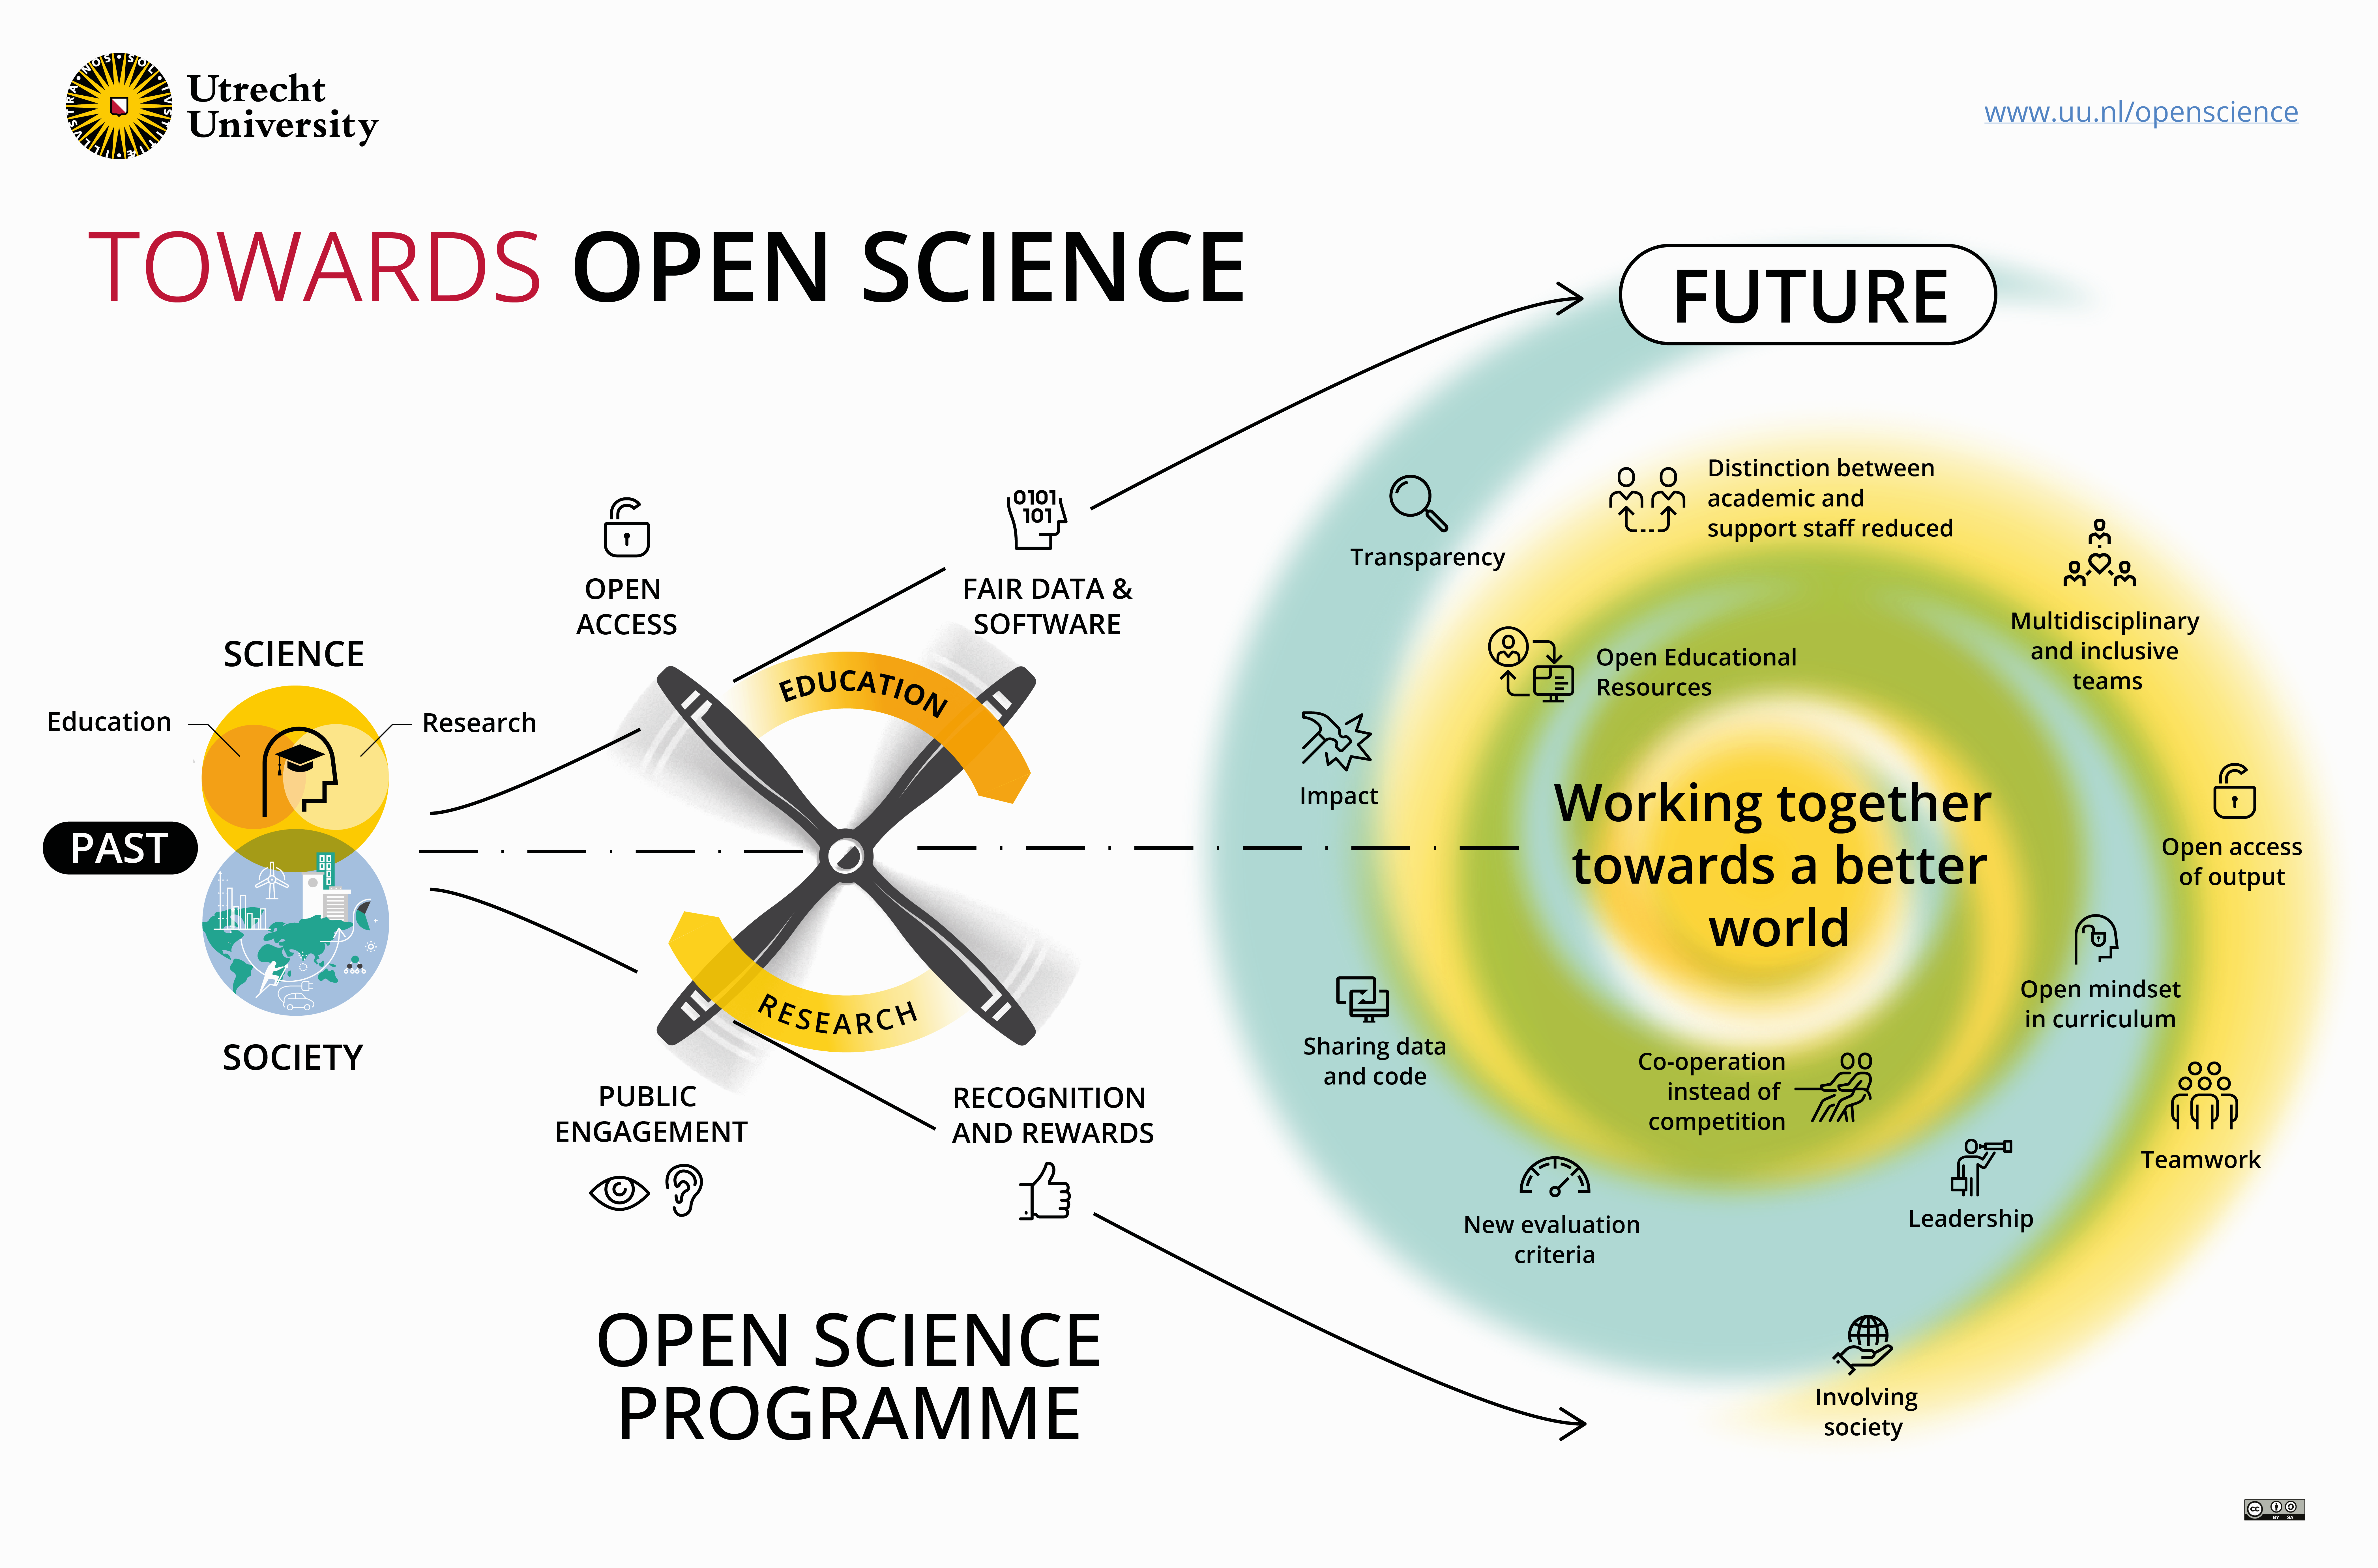
\includegraphics[width=\linewidth]{media/image1.png}



		\label{fig:rId12}



		\caption{De transitie naar Open Science\index{open science}.}
	\end{figure}



	\subsection{Open Acces en FAIR Open Data}



	\emph{Open Access\index{open access}} en FAIR Open Data\index{FAIR open data and software} en Software zijn internationale bewegingen die zijn voortgekomen en mogelijk gemaakt door de digitale revolutie die sinds 2000 nog steeds doorwerkt in de maatschappij, maar zeker ook in de universiteiten in de praktijk van onderzoek en onderwijs. Het hogere doel van deze twee bewegingen, is om de geproduceerde kennis, zowel artikelen als allerlei andere vormen van data en producten van onderzoek en onderwijs, beschikbaar te maken voor een hele brede groep stakeholders, zoals collega's, maar ook andere disciplines en instituties en bedrijven, waar ook ter wereld. Het idee is dat kennis geproduceerd met publieke middelen ‘\emph{a common }\emph{good}' is, die zo snel mogelijk beschikbaar moet komen in en voor de samenleving.\footnote{Dit is een van de normatieve uitgangspunten, idealen van de klassieke wetenschapssociologie van Merton uit de het midden van de vorige eeuw. Miedema, \emph{Science}\emph{ 3.0}\emph{, }Hoofdstuk 4.} Dit leidt tot complexe vraagstukken die te maken hebben met de rol van commerciële uitgevers die academische tijdschriften en boeken uitgegeven. Die artikelen zijn alleen toegankelijk voor lezers met abonnementen, (vaak via universiteitsbibliotheken).



	De transitie naar \emph{Open Access\index{open access}} is sinds een paar jaar in een stroomversnelling gekomen. Waren het sinds 2002, ‘\emph{position}\emph{ papers}' en ‘\emph{d}\emph{eclarations}' en vooral lokale acties verspreid over Europa, Noord en Zuid-Amerika, Australië en Afrika, sinds 2015 is er een aantal brede institutionele initiatieven. Het prominentste voorbeeld hiervan is PlanS van CoalitionS, een internationale coalitie van publieke en non-profit organisaties die onderzoek subsidiëren en de eis stellen dat resultaten meteen \emph{Open Access\index{open access}} moeten worden gepubliceerd.\footnote{https://www.coalition-s.org/} CoalitionS is in 2018 gestart vanuit Europa door Science Europe, de EU en de Wellcome Trust, maar heeft intussen ook leden uit andere continenten, zoals de Bill and Melissa Gates Foundation en Howard Hughes Medical Institute. Zeer recent heeft ook de Amerikaanse overheid de eis geïntroduceerd dat artikelen die voortkomen uit door de overheid betaald onderzoek meteen \emph{Open Access\index{open access}} beschikbaar moet komen.\footnote{https://www.science.org/content/article/white-house-requires-immediate-public-access-all-u-s--funded-research-papers-2025}



	Deze acties zijn ingegeven door het feit dat via commerciële uitgevers kennis, in artikelen en boeken, niet vrijelijk beschikbaar is. Maar ook door de exorbitante prijsstijgingen van abonnementen op elektronische tijdschriften en de daaraan gekoppelde commerciële belangen. Artikelen en onderzoekdata zijn hierdoor voor onderzoekers en publiek(en) die over minder financiële middelen kunnen beschikken nog slechter bereikbaar geworden. Zij kunnen de abonnementen niet betalen.



	Bij PlanS is eerst vooral ingezet op publicatie in \emph{Open Access\index{open access}} tijdschriften met betaling van de ‘\emph{Article}\emph{ Processing Charge}' (APC). Hierbij betalen auteurs en hun instituten voor het door de uitgever \emph{Open Access\index{open access}} maken van hun artikelen. Artikelen zijn hierdoor voor de lezers gratis toegankelijk. Ook is publicatie op zogeheten ‘\emph{repositories}', aangemoedigd. Dit heeft een sterk effect gehad in het bevorderen van het debat over \emph{Open Access\index{open access}} en Open Data\index{FAIR open data and software}. Het is echter geen oplossing voor de langere termijn. APC-betaling, net als abonnementskosten voor lezers, zijn immers net zo goed een barrière maar nu voor de auteurs en hun instituten. De bedragen die betaald moeten worden voor APC zijn de laatste jaren fors gestegen, en voor de ‘high impact' tijdschriften zelfs exorbitant gestegen. Dat gaat bijvoorbeeld op voor tijdschriften met een goede reputatie omdat ze een hogere ‘\emph{Journal Impact Factor}' (JIF)\footnote{JIF is een maatstaf voor de frequentie waarmee artikelen in een bepaald tijdschrift worden geciteerd. Die frequentie bepaalt dan de status van het tijdschrift in het geheel van tijdschriften.} hebben. Denk aan \emph{Nature, }\emph{Science}\emph{, Lancet} en \emph{Cell}. Dit zijn voorbeelden van tijdschriften die hoge abonnementskosten hebben en tegen betaling auteurs in staat stellen hun artikel toch \emph{Open Access\index{open access}} te publiceren. Daarvoor betalen de auteurs dan APC, dat is ‘\emph{hybrid}\emph{ }\emph{Open Access\index{open access}}' en wat ook wel ‘\emph{double }\emph{dipping}' wordt genoemd. Kortom, dubbele inkomsten, abonnementsgelden én APC. Het is lucratief voor uitgevers die speculeren op de ‘verslaving' aan hoge JIF's bij vooral onderzoekers en leden van beoordelingscommissies uit de exacte en biomedische disciplines. Hieronder zal daar in het kader van Erkennen en Waarderen\index{erkennen en waarderen} nader op worden ingegaan.



	Doordat we te maken hebben met een kloof tussen rijke landen in het Noordwesten en arme landen in ‘The Global South\index{global south}', maar ook in Oost-Europa, worden de laatsten ook in de wetenschap en de transitie naar \emph{Open }\emph{Science} op achterstand worden gezet. De rijkere onderzoekers die per se in ‘hun favoriete tijdschrift' willen publiceren, kunnen zich zelfs een extreem hoge APC veroorloven. Onderzoekers uit bijvoorbeeld Zuid-Amerika of Afrika die in die tijdschriften willen publiceren kunnen dat maar zelden betalen. Het is daarnaast ook goed om te beseffen dat in het algemeen ook in het rijke Westen financiële mogelijkheden tussen academische disciplines historisch zeer ongelijk zijn, bijvoorbeeld tussen de biomedische en natuurwetenschappen in vergelijking met de geesteswetenschappen.



	In 2022 is daarom de roep van CoalitionS om in de transitie naar \emph{Open Access\index{open access}} voorbij het model van APC's te gaan en nu echt naar niet-commerciële publieke \emph{Open Access\index{open access}} publicatieplatformen te gaan.\footnote{https://www.coalition-s.org/diamond-unearthed-shining-light-on-community-driven-open-access-publishing}\textsuperscript{,}\footnote{https://zenodo.org/record/4562790\#.YgeZ2\_XMIlI} Die publicatiekanalen moeten dan gefinancierd worden uit centrale publieke middelen, waarbij \emph{Open Access\index{open access}} standaard is en er via peer review\footnote{Liefst ‘\emph{open peer review}', waarbij de namen van auteurs en reviewers bekend zijn.}, toetsing is van kwaliteit. Onze collega's uit Zuid-Amerika herinneren ons er voortdurend aan dat dit bij hen als sinds jaar en dag het dominante model is, wat door PlanS met de APC's wordt bedreigd.\footnote{https://theconversation.com/latin-america-could-become-a-world-leader-in-non-commercial-open-science-161019}



	Hierbij dient te worden opgemerkt dat er een sterke verantwoordelijkheid is van het team van onderzoekers voor de kwaliteit van hun werk, maar die ligt zeker ook bij het instituut. De reputatie van een instituut zou niet moeten afhangen van de JIF, die niet correleert met de werkelijke impact en kwaliteit, maar met de intrinsieke kwaliteit en werkelijke impact van onderzoeksresultaten, data en claims en andere producten van onderzoek die vanuit het instituut worden gepubliceerd, op een ‘\emph{Diamond}' platform of een ‘\emph{prepublication}\emph{ }\emph{repository}'\footnote{Een archief/opslagplaats van data of artikelen bevat de die nog niet \emph{peer }\emph{reviewed} zijn of geaccepteerd door tijdschriften.}, en in boeken en tijdschriften. Het alleen passeren van peer review, zo is algemeen aangetoond, is niet een betrouwbaar kwaliteitskeurmerk per se.



	FAIR Open Data\index{FAIR open data and software} en Software is het publiceren en dus bruikbaar en betrouwbaar (FAIR) beschikbaar maken van onderzoekdata en software en code. Dit is terecht al veel aandacht en is een belangrijk onderdeel van wat een universiteit moet doen in het bevorderen van \emph{Open }\emph{Science}. Het stimuleert de interdisciplinaire samenwerking tussen collega's op onderzoek en onderwijs, en de interacties met de verschillende partijen in de wereldwijde samenleving. Afgezien van de enorme financiële, technische en facilitaire aspecten en voorwaarden die geadresseerd moeten worden om dit voor de medewerkers van de kennisinstellingen en de potentiële gebruikers mogelijk te maken, zijn er ethische en politieke overwegingen waar we rekening mee moeten houden. Het ethisch verantwoord open maken van datasets kan stuiten op terechte wettelijke beperkingen en bezwaren van privacy en mogelijk misbruik voor onder andere militaire doelen. Daarom is het adagium: ‘Open wanneer het kan, gesloten wanneer het moet'.

	\begin{bookbox}{\raggedright tekstbox 2 - 1. \\de verschillende vormen van open access\index{open access} publishing}
		Er zijn verschillende vormen van \emph{Open Access\index{open access}}:

		\vspace*{\baselineskip}

		\emph{Gold }\emph{Open Access\index{open access}}: publicatie in een volledig \emph{Open Access\index{open access}}-tijdschrift dat geen abonnementskosten in rekening brengt. Meestal rekenen gold \emph{Open Access\index{open access}}-tijdschriften publicatiekosten, ook wel bekend als Artikel Processing Charges (APC's).

		\vspace*{\baselineskip}

		\emph{Hybrid }\emph{Open Access\index{open access}}: publicatie in een ‘traditioneel' abonnementsblad dat \emph{Open Access\index{open access}} publicatie voor individuele artikelen aanbiedt tegen betaling van een Artikel Processing Charge (APC).

		\vspace*{\baselineskip}

		\emph{Green }\emph{Open Access\index{open access}}: publicatie in een gesloten tijdschrift en vervolgens archivering van een versie van de publicatie in een vertrouwde \emph{Open Access\index{open access}} \emph{repository}. Publicaties kunnen worden gearchiveerd bij publicatie of daarna, afhankelijk van het beleid van het tijdschrift. Vaak is het zelf archiveren van de\emph{ }\emph{final}\emph{ }\emph{author's}\emph{ }\emph{version}\emph{ (post-print}\emph{)} na een embargoperiode toegestaan.

		\vspace*{\baselineskip}

		\emph{Diamond}\emph{ }\emph{Open Access\index{open access}}: publicatie in een volledig \emph{Open Access\index{open access}}-tijdschrift of platform dat geen publicatiekosten (APC's) in rekening brengt. De kosten voor publicatie en hosting worden gedragen door één of meer organisaties, verenigingen of netwerken.
	\end{bookbox}

	Net als bij \emph{Open Access\index{open access}} zijn er terecht ook zorgen over de ongelijke machtsverhoudingen op nationaal niveau en in de wereld.\footnote{https://www.unesco\index{UNESCO}.org/en/natural-sciences/open-science} We hebben tijdens de COVID-19\index{COVID-19} pandemie de enorme impact gezien die het delen van data op internationaal niveau kan hebben, toen het meteen delen van genetische informatie over het virus en het publiceren van ruwe data waarop publicaties waren gebaseerd even normale praktijk waren. Ook op het gebied van onderwijs, de \emph{computer }\emph{sciences}, \emph{cybersecurity} en onderzoek van energie en klimaat zijn er mooie voorbeelden. Er zijn tegelijkertijd zorgen. Het delen van data en code zal de onderzoekers en het publiek uit rijke landen bevoordelen ten opzichte van inwoners van armere landen, want ze hebben meer gelegenheid die informatie te benutten, omdat er in rijke landen meer financiële middelen zijn voor hergebruik en commerciële en andere profijtelijke toepassingen. Dit zijn geen nieuwe problemen die zich in de universiteit openbaren, maar problemen waarmee de academie ook in andere tijden heeft geworsteld. Denk bijvoorbeeld aan de jaren 1939 tot 1945 rond de ontwikkeling van de atoombom en daarna in de verhouding met de Sovjet-Unie tijdens de koude oorlog. Voor de meesten van ons is dat, zeker sinds 1989, een ver verleden, maar het bestuderen van die specifieke geschiedenis van de interacties van wetenschap en samenleving is nu zeer verhelderend en geeft inzichten voor de huidige geopolitieke discussies; ook tijdens de koude oorlog werden bewust resultaten van bepaald wetenschappelijk onderzoek niet verder verspreid. Deze structurele politiek sociaaleconomische ongelijkheid is van algemene aard die we moeten anticiperen en zoveel mogelijk moeten mitigeren in de context van \emph{Open Data\index{FAIR open data and software}} en \emph{Code} in \emph{Open }\emph{Science}.



	Een ander risico is het op een naïeve manier delen van data met partijen die daar misbruik van zouden kunnen maken. Dat kan gaan om toepassing van data of code voor politieke en ethisch ongewenste praktijken. Dit kan niet altijd voorkomen worden, maar de onderzoeker die de data of code heeft geproduceerd moet hier steeds zeer alert op zijn. De discussies over het delen van data en code met partijen in landen met autoritaire regeringen die de data en code voor militaire of onderdrukkende doelen. Geopolitiek speelt hier ook weer een rol. Dus is ook hier het adagium: ‘Open wanneer het kan, gesloten wanneer het moet'. We moeten constateren dat er in de wereld anno 2022 niet maar één wetenschap, met één set van normen en waarden bestaat en dat \emph{Open }\emph{Science} afhankelijk is van een Open Society met een open democratie en niet of veel minder goed functioneert in landen waar daar niet aan voldaan wordt.



	\subsubsection{Open Innovation}



	Bij het delen van data in een ‘\emph{international}\emph{ community of }\emph{inquirers}' moeten afspraken gemaakt worden over hoe de betrokken partijen hiervan kunnen profiteren. Er zijn voorbeelden van geneesmiddelenontwikkeling waarbij universiteiten, die kennis en patenten hebben ontwikkeld, en farmaceutische bedrijven die het geneesmiddel naar de markt willen brengen, tijdig afspraken maakten over hoe, waar en tegen welke prijs die geneesmiddelen beschikbaar zouden komen. Hierbij kunnen dan lage prijzen worden bedongen voor \emph{Low }\emph{and}\emph{ }\emph{Middle-Income-Countries}. Dat wijkt af van de neoliberale\index{neoliberaal} vrijemarkteconomie waar we in de westerse wereld zijn terecht gekomen en is dus een moeizame maar belangrijke nieuwe weg die we op moeten gaan.\footnote{\href{https://www.nfu.nl/themas/randvoorwaarden-wetenschappelijk-onderzoek/valorisatie}{https://www.nfu.nl/themas/randvoorwaarden-wetenschappelijk-onderzoek/valorisatie}; ‘Maatschappelijk verantwoord licentiëren'.} Er zijn daarnaast veel initiatieven wereldwijd die Open Innovation stimuleren tussen bedrijven en academische partners, Novo Nordisk Foundation is een voorbeeld.\footnote{\href{https://www.novonordisk.com/partnering-and-open-innovation/open-innovation.html}{https://www.novonordisk.com/partnering-and-open-innovation/open-innovation.html} }



	De onderliggende structurele maatschappelijke ongelijkheid hangt samen met geopolitieke, nationale en maatschappelijke structuren die veel van deze zaken bemoeilijken of onmogelijk maken en niet bepaald worden door de academie, maar die de universiteit wel steeds kritisch moet beschouwen en internationaal hoog op de agenda zal moeten houden.



	\subsection{Public Engagement: Science with and for Society\index{science with and for society} }



	Public Engagement\index{public engagement} heeft veel vormen en kent een enorme variatie aan resultaten. Het klassieke voorbeeld is zogeheten ‘\emph{Citizen}\emph{ }\emph{Science}' en betreft burgers, niet-academische onderzoekers die meedoen in wetenschappelijk onderzoek, door bijvoorbeeld observaties te doen en data te verzamelen. Public engagement\index{public engagement} gaat echter veel verder. Het betreft onderzoek dat gebaseerd is op een onderzoekvraag die door onderzoekers samen met burgers is geformuleerd en vertaald in een onderzoeksproject dat gezamenlijk wordt uitgevoerd. Daarbij wordt dan meestal ook de nieuwe kennis, en/of het nieuw ontwikkelde product getest in de context waarin de vraag van de burgers vandaan komt. Ook kunnen door publieke participaties nieuwe onderwijsmethoden en middelen worden ontwikkeld die aansluiten op maatschappelijke problemen. In alle academische disciplines zijn prachtige voorbeelden van deze participatiewetenschap beschreven, van geneeskunde, de psychiatrie, onderwijskunde, internationaal recht, lokale politieke problemen ten aanzien van door menselijk handelen veroorzaakte de schade aan milieu, leefomgeving en welzijn, gelijke behandeling (inclusiviteit\index{inclusiviteit}) in allerlei maatschappelijke situaties zoals het onderwijs.



	Hierbij staat voorop dat de betrokken onderzoekers ervan overtuigd zijn dat die co-creatie tot bruikbare resultaten kan leiden, die daadwerkelijk de potentiële gebruikers zal bereiken. Dit wordt ondersteund door veel empirisch onderzoek. Als een onderzoeker niet alleen eventuele resultaten wil toepassen in de maatschappij, maar ook al vanaf het zeer vroege begin bij de vraag articulatie samen optrekt, verkleint dat de afstand tussen de onderzoeker en de potentiële gebruiker, met maximale kans op het maken van impact. Afstand kan hier de betekenis van fysieke afstand hebben, van fysiek met elkaar samenwerken, maar ook die van geestelijke afstand, elkaar begrijpen.

	\begin{bookbox}{\raggedright tekstbox 2 - 2. \\over het masterprogramma ‘global challenges for sustainability’}
		Een voorbeeld van \emph{public engagement\index{public engagement}} waarbij maatschappelijke actoren een onderzoeksvraag formuleren waar onderzoekers, maatschappelijke actoren en studenten gezamenlijk mee aan de slag gaan, vindt plaats binnen het CHARM-EU masterprogramma ‘\href{https://www.charm-eu.eu/masters/globalchallenges}{\emph{Global }\emph{Challenges}\emph{ }\emph{for}\emph{ }\emph{Sustainability}}'. In dit allereerste Europese \emph{joint }\emph{degree} masterprogramma volgen studenten tegelijkertijd in vijf universiteiten hybride onderwijs dat gelinkt is aan uitdagingsgericht transdisciplinair onderzoek. Tijdens de \href{https://www.charm-eu.eu/capstonephase}{\emph{Capstone}}, de laatste fase van het masterprogramma die de Universiteit Utrecht coördineert, formuleren maatschappelijke actoren (bedrijven, NGO's, overheidsinstanties, etc.) een duurzaamheidsuitdaging waarvoor zij een oplossing zoeken. Studententeams van de vijf CHARM-EU partneruniversiteiten werken onder begeleiding van onderzoekers en maatschappelijke actoren aan het analyseren van het probleem en het formuleren van oplossingen, aanbevelingen en/of prototypes. De duurzaamheidsuitdagingen verschillen per jaar en lopen uiteen in disciplines en geografische focus binnen en buiten Europa. Sommige uitdagingen hebben betrekking op mondiale kwesties, zoals de manier waarop de Verenigde Naties bedrijven kan adviseren en stimuleren de duurzame ontwikkelingsdoelstellingen te implementeren en monitoren. Andere uitdagingen zijn gericht op lokale kwesties, waarbij een van de \emph{Capstone} teams een smartphone app heeft ontworpen om burgers in Utrecht te enthousiasmeren om stadsboerderijen en stadstuinen op een speelse en leerzame manier te ontdekken. In Zuid-Afrika werken \emph{Capstone} teams aan het analyseren en aanpakken van conflicten tussen mensen, vee en wilde dieren rond het Kruger National Park. Daarbij begint het team met het formuleren van een probleemstelling op basis van gesprekken met de leiders van de lokale gemeenschap\index{gemeenschap} en andere stakeholders in het park. Dit vergt flexibiliteit, interdisciplinariteit en culturele sensitiviteit om problemen van meerdere kanten en op lokaal geaccepteerde wijzen te analyseren en adresseren. Wetenschappelijke en inheemse kennis wordt vervolgens geïntegreerd en gedeeld door een lokaal transdisciplinair\index{transdisciplinair} onderzoekscentrum, een satellietcampus van de Universiteit van Pretoria. Dit onderzoekscentrum voert onderzoek en trainingen uit rond het tegengaan van ziektes in de veestapel, natuurbehoud en duurzame manieren van leven in het park. Op die manier wordt er niet alleen internationaal erkend onderzoek gedaan, maar vindt er ook lokale capaciteitsopbouw plaats en worden er innovatieve oplossingen ontworpen voor lokale problemen die ook grensoverschrijdend zijn. De onderwijsmethoden in de \emph{Capstone} zijn ontwikkeld onder leiding van de Universiteit Utrecht door een transdisciplinair\index{transdisciplinair} team van onderzoekers en docenten van de vijf partneruniversiteiten in samenwerking met maatschappelijke actoren. Dit zorgt voor een directe aansluiting van het onderwijs en onderzoek op maatschappelijke vraagstukken, en resulteert in gezamenlijke leerprocessen van alle betrokkenen. CHARM-EU is een Europese universiteitsalliantie die fungeert als een testbed voor \href{https://www.charm-eu.eu/torch}{innovaties en institutionele veranderingen} ten behoeve van \emph{Open }\emph{Science} en Public Engagement\index{public engagement} in het onderwijs en onderzoek van de inmiddels negen CHARM-EU partnerinstellingen.
	\end{bookbox}

	Er is nu een keur aan \emph{Open }\emph{Science} \emph{Declarations}, aanbevelingen, implementatieplannen en strategieën van de EU, de UN en UNESCO\index{UNESCO}, overheden, en velerlei instituties overal ter wereld. De meeste onderzoekers, en de meeste universiteiten in 2022 zijn, in de geest van \emph{Open }\emph{Science}\emph{,} van mening dat een fors deel van het onderzoek een bijdrage zou moeten leveren aan het helpen oplossen van problemen in de samenleving.\footnote{In dat verband zijn ook de initiatieven rond RRI (‘\emph{Responsible}\emph{ Research }\emph{and}\emph{ }\emph{Innovation}') in de context van de Europese Kaderprogramma's van belang: https://tetrris.eu/what-is-responsible-research-and-innovation-rri/} Heel veel onderzoek wordt gedaan om te helpen bij het nemen van de juiste beslissing bijvoorbeeld in een politiek debat. Dat betekent dat universiteiten en hun medewerkers in het onderzoek en het onderwijs bewust keuzes maken voor onderwerpen en problemen die om onderzoek en nieuwe vormen van onderwijs vragen. Universiteiten zullen in deze transitie, veel meer dan nu al het geval is, in een inhoudelijk en organisatorisch proces naar een thematische profilering van hun onderzoek gaan.



	\subsection{Profilering}



	Universiteiten, willen ze optimaal hun doelen halen, zullen in de grote thema's moeten bepalen op welke onderwerpen zij vanuit hun kracht maximaal waarde kunnen toevoegen en optimale impact kunnen hebben in de academie en in de maatschappij. Vanuit hun strategie zal in de komende decennia hun onderzoek en hun kwaliteit en excellentie worden beoordeeld, niet door het aantal publicaties in \emph{Science} en \emph{Nature}, maar juist op de werkelijke academische en maatschappelijke waarde en impact. Dat brengt universiteiten en onderzoekers heel dicht bij de publieke, private en politieke arena en roept prangende vragen op over de relatie van universiteiten met de samenleving. Dat gaat over de klassieke thema's, waardevrije wetenschap, neutraliteit maar ook over verantwoordelijkheid ten aanzien van de samenleving. Het gaat over welke algemene en mogelijk ook meer lokale waarden en normen de universiteit dan moet propageren.



	De onderzoeker komt mensen tegen met uiteenlopende opvattingen, angsten, ervaringen, wensen, politieke overtuigingen en een onderliggend patroon van normen en waarden. Dat beïnvloedt deze burgers sterk in de interpretatie van en de discussies over het wetenschappelijk werk. Denk maar aan de aanpak van de covidpandemie, of de stikstofcrisis. Een deel van de burgers zal zich niet gesteund voelen door de informatie die wetenschappers ter tafel brengen. Veelal zal gewezen worden op onderzoekers die andere claims en feiten presenteren dan de consensus., en op de verschillen in context, waarin het onderzoek is gedaan. Verschillen ten aanzien van de onderzoekscontext, en de werkelijke omgeving waar de resultaten van onderzoek gedacht worden van toepassing te zijn, zijn van belang. Hierdoor wordt op verschillende wijze bewijskracht voor de wetenschappelijke claims in twijfel getrokken. Deze manier van argumenteren is vergelijkbaar met hoe advocaten in rechtszaken bewijs deconstrueren naar vooringenomen ideeën, context afhankelijke aannames, interpretaties en methoden. Dat zijn dus wezenlijk andere discussies dan discussies die de onderzoeker met vakgenoten heeft over haar werk, waar cognitieve (‘wetenschappelijke') argumenten de overhand hebben en vaak ‘netjes' gescheiden blijven van die oordelen over het werk vanuit allerlei maatschappelijke, sociaaleconomische, politieke en culturele overwegingen.\footnote{Jasanoff, ‘What Judges Should Know', 345-59.}\textsuperscript{,}\footnote{Jasanoff, \emph{Science}\emph{ }\emph{and}\emph{ Public }\emph{Reason}.} Netjes gescheiden in de zin dat in academische discussies beide partijen trachten het cognitieve te scheiden van niet-cognitieve normen en waarden, waarbij de laatste categorie vaak buiten beeld kan blijven.



	In de tijd van het positivisme van 1930 tot 1970, met het nu nog vaak dominante klassieke beeld van wetenschap, werden de grenzen tussen de werelden van burgers en wetenschap veelal kunstmatig strikt gescheiden. Invloed op de wetenschap, welke dan ook, van buitenaf was taboe. Echter, toen, maar zeker ook in onze moderne tijden ontwikkelden de wetenschap en de samenleving zich beide continue en parallel aan elkaar en heel snel. Daarbij is er een constante wisselwerking en wederzijdse beïnvloeding, waarbij beide reageren en anticiperen op elkaars ‘gedrag', ideeën, communicatie en acties in de publieke sfeer waar burgers, onderzoekers en politici verkeren. Dit heeft vaak direct en indirect effect op de voortgang van wetenschappelijk onderzoek. Recente wetenschapsfilosofische inzichten laten zien dat onderzoekers in hun onderzoek en academische debatten onbewust altijd vanuit hun sociaal culturele context, met hun normen en waarden functioneren, en dat die juist heel belangrijk kunnen zijn in het onderzoek en dat die maar beter geëxpliciteerd en ter discussie gesteld kunnen worden.\footnote{Zie de discussie over het werk van Shapin en Longino in Miedema, \emph{Open }\emph{Science}, 15-66.}



	\subsection{Reflexiviteit}



	Het werkelijk begrijpen en invoelen van het probleem dat een burger, patiënt, kind met een immigratie achtergrond, onderwijzer, CEO of ambtenaar heeft, en wat dat voor de positie, attitude en betrokkenheid van de onderzoeker betekent, is van het grootste belang voor de kwaliteit van participatief onderzoek en Public Engagement\index{public engagement}.



	Het gaat dus in hoge mate ook over de reflectie van de universiteit en de onderzoeker op hun eigen positie in de betreffende maatschappelijke context van onderzoek en de eigen ervaringen, verwachtingen, normen en waarden.



	Onderzoekers worden geconfronteerd met tegenspraak, ‘\emph{society }\emph{speaks}\emph{ back}' en er is een grote mate van onzekerheid over de status van onze wetenschappelijke kennisclaims. De klassieke autoriteit is verdwenen. Die autoriteit was, zoals elders uitgebreid is bediscussieerd, gebaseerd op een geïdealiseerd beeld van de wetenschap (‘\emph{The Legend}') dat nu vervangen is door een realistisch narratief over hoe we in de wetenschap tot kennisclaims komen en hoe die door constante discussie en onderzoek steeds getest, verworpen of verbeterd worden.\footnote{Miedema, \emph{Open }\emph{Science}\emph{.}} Het gaat in interacties niet om het beroep op absolute kennis of feiten, maar op aantoonbare ‘robuuste en betrouwbare' kennis die zijn waarde bewezen heeft in continue discussie met collega's en in acties en interventies in het lab, een testomgeving, een klinische trial, maar ook in de echte wereld. Ten aanzien van dat laatste is het van groot belang dat de onderzoeker zich bewust is dat kennis en kennisclaims altijd in een bepaalde omgeving, ‘\emph{setting}', maatschappelijke en culturele context zijn geproduceerd en gevalideerd. In de geneeskunde is hier veel en teleurstellende ervaring mee ten aanzien van werkzaamheid van geneesmiddelen. Deze zijn vaak getest en gevalideerd in experimenten en trials waarin veelal patiënten deelnamen die streng geselecteerd zijn op leeftijd, geslacht, etniciteit en bepaalde ziektekenmerken. Hierdoor zijn ze niet altijd representatief, voor vrouwen of mensen die uit andere continenten komen.\footnote{Epstein, \emph{Inclusion}.} Voor antidepressiva, maar ook voor geneesmiddelen in de oncologie, cardiologie en patiënten met afweerstoornissen zijn hier voorbeelden van. Een ander mooi voorbeeld is in de geneeskunde ten aanzien van de geheel verschillende verspreiding van HIV in Sub-Sahara Afrika vergeleken met Amsterdam en San Francisco. In Sub-Sahara Afrika is de verspreiding niet via homoseksuele contacten maar vooral via heteroseksuele contacten. Men dacht hier eerst alleen maar vanuit ons Westers referentiekader met haar dominantie van sequentiële heteroseksuele relaties met de kans op verspreiding die positief gecorreleerd aan de frequentie en aard van heteroseksuele contacten. Dat bleek geen plausibele verklaring in Afrikaanse landen met enorme heteroseksuele hiv-verspreidingen. Door contacten met antropologen en sociologen in Afrika kwam de relatief late ‘ontdekking' van de oorzaak van dit verschil. Het bleek dat in die Afrikaanse landen van oudsher totaal verschillende cultureel bepaalde heteroseksuele relaties dominant waren en nog steeds zijn. Deze netwerken van gelijktijdige, meervoudige seksuele relaties van mannen en vrouwen kon een snelle verspreiding onder mannen èn vrouwen via heteroseksuele contacten verklaren. Dit verklaarde ook de veel grotere verspreiding van HIV onder jonge en pasgeboren kinderen.\footnote{Miedema, \emph{Wetenschap 3.0}, Hoofdstuk 9. }



	\subsection{Erkennen en Waarderen}



	Door de institutionele transitie naar \emph{Open }\emph{Science} zoals hiervoor beschreven, is in de EU en elders in de wereld snel duidelijk geworden dat voor een succesvolle blijvende transitie en implementatie de manier van evalueren en belonen van onderzoekers en onderzoek moet worden aangepast. Dat systeem door Robert Merton in het midden van de vorige eeuw al met ‘\emph{reward}\emph{ system}' aangeduid, moet worden gemoderniseerd.\footnote{Merton, \emph{Sociology}\emph{ of }\emph{Science}\emph{.}} Als we zoals hieronder ‘\emph{the}\emph{ }\emph{credibility}\emph{ }\emph{cycle}' in beeld nemen zien we in één oogopslag hoe dat in de dagelijkse praktijk zijn uitwerking heeft. Op meerdere plekken in de cirkel zijn criteria en de daarvan afgeleide indicatoren zeer bepalend voor onze oordelen over kwaliteit en daardoor bepalend voor het toekennen van subsidies en van prijzen.\footnote{Hessels et al., ‘In Search of Relevance', 387--401.} Deze indicatoren spelen een grote rol in het werven van wetenschappers, besluiten ten aanzien van academische benoemingen, vaste contracten en promotie naar bijvoorbeeld UD, UHD of Hoogleraar.\footnote{Moher et al., ‘Assessing Scientists'.} Zoals de figuur laat zien is het systeem van Erkennen en Waarderen\index{erkennen en waarderen} te beschouwen als het ‘verdienmodel' van de moderne wetenschap. Door de indicatoren en criteria die wereldwijd expliciet en soms impliciet worden gebruikt, worden begrippen als kwaliteit en excellentie gedefinieerd en is er een voor iedereen herkenbare hiërarchie in de academische disciplines. Hier ligt een ware uitdaging voor de universiteit de komende jaren, ook ten aanzien van de enorme en nog steeds groeiende hypercompetitie voor academische posities aan de universiteit en voor subsidies en de daarmee gepaard gaande aanvraagdruk en natuurlijk de werkdruk en belasting bij de aanvragers.



	Vele auteurs hebben sinds 2000 laten zien hoe het systeem van Erkennen en Waarderen\index{erkennen en waarderen} zich heel snel sinds de negentiger jaren heeft ontwikkeld.\footnote{Wouters, ‘The Citation', 47-66.} Elders zijn recent in detail de klassieke visies op wetenschap besproken, die Ziman en Kitcher \emph{‘The Legend'} hebben genoemd, die ten grondslag liggen aan dat evaluatiesysteem. De box hieronder maakt duidelijk waarom het dominante evaluatiesysteem de transitie naar \emph{Open }\emph{Science} niet zal faciliteren, laat staan bevorderen.



	\begin{figure}
		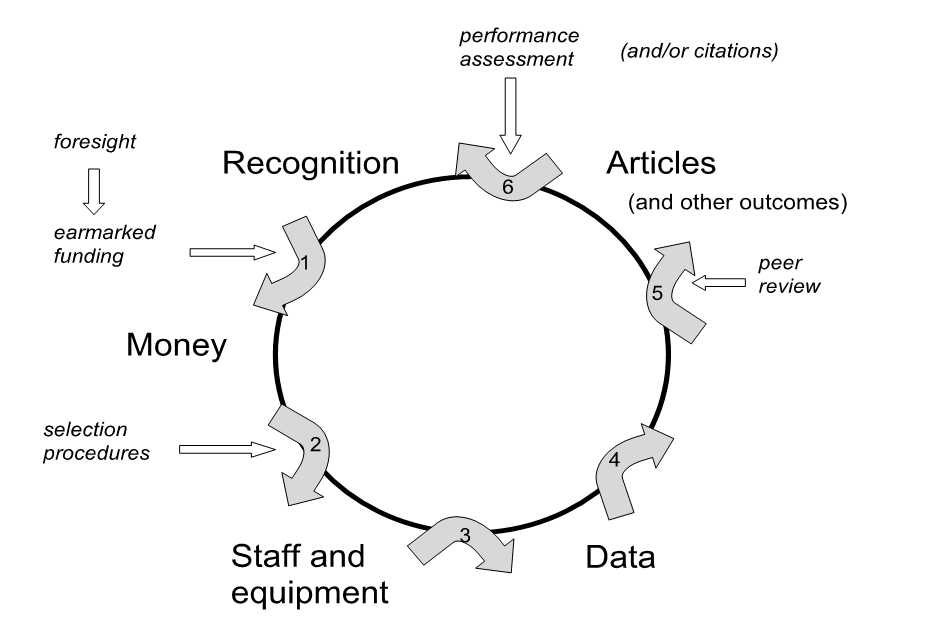
\includegraphics[width=\linewidth]{media/image2.png}



		\label{fig:rId16}



		\caption{The credibility cycle, overgenomen van Latour en Woolgar (1986). Shown are points at which organizational devices connect to the cycle.}
	\end{figure}



	Nu is het, ondanks dit gegeven, sinds 1995 de gewoonte geworden om de Journal Impact Factor ook te gebruiken voor het bepalen van de kwaliteit van het werk van individuele artikelen en de kwaliteit van hun auteurs. De editors en hun ‘\emph{associate}\emph{ editors}' sturen op het verwerven van artikelen die geheid grote aandacht kunnen trekken door dat het onderzoek bijvoorbeeld heel fundamenteel is of heel actueel en nieuw en baanbrekend. Dat trekt immers de algemene aandacht binnen en buiten de wetenschap. Hier spelen de klassieke visies en ideologieën van wetenschap een hoofdrol. Door de aandacht en citaties hopen de editors een nog hogere JIF voor hun tijdschrift te verkrijgen. Hieraan is de reputatie van het tijdschrift gekoppeld, maar ook de ‘\emph{subscription}\emph{ }\emph{and}\emph{ APC fee'} Voor \emph{Nature} is het laatste al opgelopen tot boven de 10.000 euro. Zie hier het verdienmodel van de commerciële uitgevers.



	De JIF en de reputatie van een tijdschrift spelen, ondanks de evidente foute basis, een enorm bepalende rol in vooral de exacte disciplines en het grote gebied van de biomedische wetenschappen, maar dat heeft intussen ook navolging gekregen in de economie en zelfs de sociale wetenschappen.



	De LEGEND laat zich het best zo karakteriseren:

	\begin{quote}
		\itshape

		‘There is a unique “scientific method” that guarantees objective truth of general, universal and timeless theories and claims. These claims allow understanding, prediction and control of our world (nature/men). The method is logical-empirical and has a firm foundation. Facts and values; science and non-science are neatly separated, which makes science objective and neutral. This method explains the success of the “hard” sciences; the “soft” social sciences and humanities are methodologically problematic'.\footnote{Miedema, \emph{Open }\emph{Science}\emph{.}}
	\end{quote}

	\subsubsection{\emph{Metrics shape Science}}



	Wat impliceert het dat de \emph{metrics\index{metrics}} bepalend zijn? Daarmee moet men denken aan alles wat zich in de ‘\emph{credit }\emph{cycle}\emph{'} afspeelt: via peer review in zo'n tijdschriftartikelen geaccepteerd krijgen, op basis daarvan excellentie toegemeten krijgen, op basis daarvan onderzoeksubsidies, en academische posities verkrijgen en vervolgens via het zogenaamde Matthew Effect betere toegang tot jarenlang mooie en forse eervolle subsidies. Er is al zeker tien jaar brede internationale kritiek op het gebruik van deze \emph{metrics\index{metrics}}. Experts hadden dat overigens al veel langer. De\emph{ }\emph{Declaration}\emph{ on Research Assessment} (DORA) is een internationale beweging, gestart in 2012, door vele instituten en personen ondertekend, die het gebruik van de JIF op deze manier verbiedt. De implementatie daarvan in de instituten is pas sinds 2015 serieus opgang komen en maakt deel uit van het Erkennen en Waarderen\index{erkennen en waarderen} project in vele instituten.\footnote{The Declaration on Research Assessment (DORA): \href{https://sfdora.org/}{https://sfdora.org/} }



	DORA is gericht op dit apert foute gebruik van ‘\emph{poor}\emph{ }\emph{proxies}\emph{ }\emph{for}\emph{ }\emph{quality}\emph{ }\emph{and}\emph{ excellence}' en op verbreding van de criteria voor beoordeling en evaluatie. Het is echter niet alleen een probleem is voor de academie. We moeten ons realiseren dat veel onderzoek met hele hoge kwaliteit en grote wetenschappelijke en of maatschappelijk impact niet interessant is voor de tijdschriften met die hoge JIF en dat zelfs in commissies die zeer verschillende onderzoeksvoorstellen moeten beoordelen voor subsidiegevers de JIF bepalend is. Dat betekent dat hierdoor de keuze voor onderzoek in een aantal grote disciplines en domeinen niet door de \emph{werkelijke} kwaliteit en impact bepaald wordt.\footnote{\href{https://scienceintransition.nl/over-science-in-transition/position-paper}{https://scienceintransition.nl/over-science-in-transition/position-paper}}\textsuperscript{,}\footnote{\href{https://responsiblemetrics.org/the-metric-tide/}{https://responsiblemetrics.org/the-metric-tide/}}



	\begin{figure}
		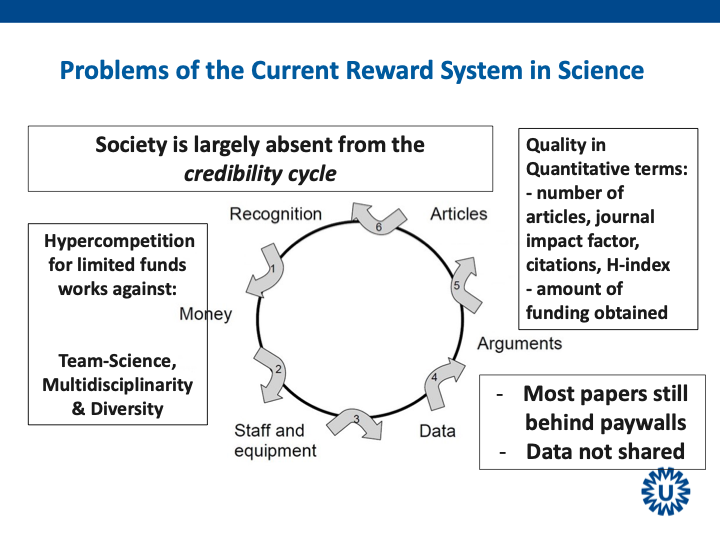
\includegraphics[width=\linewidth]{media/image3.png}



		\label{fig:rId17}



		\caption{Problemen van het huidige beloningssysteem in wetenschap.}
	\end{figure}







	In het domein van het biomedisch en gezondheidsonderzoek heeft de Gezondheidsraad op verzoek van de minister van VWS in 2016 een advies uitgebracht onder de omineuze titel ‘Onderzoek waar je beter van wordt'. Dit ministerieel verzoek was ingegeven door boven genoemde publicaties dat de research agenda te veel werd bepaald op basis van de \emph{metrics\index{metrics}} en niet op basis van maatschappelijk en klinische impact. Het advies vroeg dan ook om een aanpassing van de beoordeling van het onderzoek, en onderzoekers op basis van meer inclusieve criteria, zoals ook de maatschappelijke relevantie van onderzoek.\footnote{\href{https://www.awpgnzh.nl/wp-content/uploads/Onderzoek-waarvan-je-beter-wordt-Gezondheidsraad-2016.pdf}{https://www.awpgnzh.nl/wp-content/uploads/Onderzoek-waarvan-je-beter-wordt-Gezondheidsraad-2016.pdf} } Dit is de reden dat Erkennen en Waarderen in 2016 een integraal onderdeel is geworden van het \emph{Open }\emph{Science} programma in de EU en in vele instituties.



	Ondanks dat de vooroordelen van ‘\emph{The Legend}' filosofisch en sociologisch al decennia aangetoond zijn, zijn ze in discussies over wetenschap in de academie, bij de overheid, subsidiegevers, academische instituties inclusief de Koninklijke Academies en in de media helaas nog zeer dominant. De maatschappelijke impact en ‘\emph{societal}\emph{ }\emph{need}' van toegepaste wetenschap en technologische wetenschappen staat in de klassieke wetenschapsopvatting in lager aanzien dan ‘pure' wetenschap, de laatste ook wel ‘\emph{blue }\emph{skies}\emph{ }\emph{science}' of ‘\emph{curiosity}\emph{ }\emph{driven}\emph{ }\emph{science}' genoemd. De kwalificatie ‘\emph{curiosity}\emph{ }\emph{driven}' is suggestief en incorrect want in alle onderzoek is nieuwsgierigheid aan de orde, namelijk voor het oplossen van problemen van welke aard dan ook. In deze klassieke dichotomie is kwantitatieve formele ‘harde' wetenschap dominant over ‘zachte' kwalitatieve wetenschap, zoals in de geestes- en sociale wetenschappen. Dit ondanks de bewezen waarde van beide voor de aanpak van grote maatschappelijke problemen zoals de klimaatcrisis, de groeiende ongelijkheid en de COVID-19\index{COVID-19} pandemie.



	In Nederland is de laatste jaren veel progressie gemaakt door de UNL (voorheen VSNU), NWO\index{nederlandse organisatie voor wetenschappelijk onderzoek (NWO)}, NFU en KNAW in een ‘\emph{position}\emph{ paper}', ‘Ruimte voor ieders talent'.\footnote{\href{https://www.universiteitenvannederland.nl/files/documenten/Domeinen/Onderzoek/Position\%20paper\%20Ruimte\%20voor\%20ieders\%20talent.pdf}{https://www.universiteitenvannederland.nl/files/documenten/Domeinen/Onderzoek/Position\%20paper\%20Ruimte\%20voor\%20ieders\%20talent.pdf}} Hier een citaat:

	\enlargethispage{-\baselineskip}\checkandfixthelayout
	\begin{quote}
		\itshape

		‘Daarvoor is een systeem van erkennen en waarderen\index{erkennen en waarderen} van wetenschappers en onderzoek nodig dat:

		1. diversificatie en het dynamiseren van loopbaanpaden mogelijk maakt, zodat excellentie in ieder van de kerndomeinen wordt bevorderd;

		2. recht doet aan zowel de onafhankelijkheid en de individuele kwaliteiten en ambities van wetenschappers, als aan teamprestaties;

		3.het accent legt op de kwaliteit van het werk en minder nadruk legt op kwantitatieve resultaten (zoals aantal publicaties);

		4. alle aspecten van Open Science\index{open science} stimuleert; en

		5. hoogwaardig academisch leiderschap stimuleert.

		Open Science\index{open science}

		Meer ruimte voor Open Science\index{open science} vraagt specifieke aandacht. Deze nieuwe benadering van wetenschap geeft anderen, naast de wetenschapper zelf, de gelegenheid om mee te werken en bij te dragen aan, en gebruik te maken van het wetenschappelijk proces. Dit betekent bijvoorbeeld dat wetenschappers de resultaten van wetenschappelijk onderzoek breder delen met de samenleving, dat ze onderzoeksresultaten toegankelijk maken en dat ze de samenleving bij het onderzoek kunnen betrekken (bijvoorbeeld citizen science). Open Science\index{open science} en de modernisering van het systeem van erkennen en waarderen\index{erkennen en waarderen} zijn onlosmakelijk met elkaar verbonden. Het vraagt tijd en aandacht van de wetenschappers die niet automatisch terug te voeren zijn naar traditionele wetenschappelijke output zoals publicaties, maar die wel een grote impact kunnen hebben op de samenleving en wetenschap (bijvoorbeeld het delen van onderzoekdata).'
	\end{quote}

	In de Universiteit van Utrecht hebben we gewerkt aan een integrale inclusieve beoordeling van onze academische medewerkers in het kader van ons \emph{Open }\emph{Science} programma geheel in lijn met DORA en de bovengenoemde projecten en hun achterliggende visies. De implementatie van een dergelijk beoordelingsprotocol was op hoofdlijnen geformuleerd en dat betekent dat het nader vorm gegeven moet worden in de diverse faculteiten en afdelingen en Strategische Thema's. Dat is waar het echte werk gaat beginnen: wat is impact en kwaliteit in die zeer verschillende contexten, hoe kom je dan aan goede narratieven en criteria?











	Naast research in engere zin, is er nu dus ook veel aandacht voor onderwijs, maar ook voor academische activiteiten die te maken hebben met ‘\emph{academic}\emph{ }\emph{duties}', inspanningen die de kwaliteit van de praktijk van onderzoek en onderwijs bevorderen. Hier denken we aan peer review, commissiewerk bij subsidiegevers, maar ook aan tijdsbesteding aan bevorderen en doen van FAIR/Open Data, \emph{Open Access\index{open access}} en \emph{Public Engagement\index{public engagement}} en het bijpassende academisch leiderschap. Dit zijn activiteiten die, in juist al hun veelzijdigheid en pluriformiteit, in een moderne evaluatie van onderzoek, onderwijs en onze medewerkers een belangrijke plek moeten hebben. In andere landen zijn in nationale protocollen voor het beoordelen van onderzoek en academici deze bewegingen, soms meer soms nog wat minder, al zichtbaar en zijn er veel transities gaande.

	\begin{bookbox}{\raggedright tekstbox 2 - 3. \\het research excellence framework}
		In het Verenigd Koninkrijk is het \emph{Research Excellence Framework} (REF) (2014) een reactie geweest op de \emph{Research Assessment }\emph{Exercise} (1986-2008), die erg stuurde op de klassieke academische output van ‘\emph{science}\emph{ }\emph{for}\emph{ }\emph{science}' en weinig aandacht had voor toegepaste en de zachte wetenschappen. In de REF is nadrukkelijk aandacht en gewicht gegeven aan maatschappelijke impact in de beoordeling van universitair onderzoek. Omdat op basis van de REF-scores de onderzoeksgelden door UKRI worden verdeeld over de instituties, heeft dit direct financiële consequenties. De klassieke ‘OxBridge' universiteiten en hun epigonen kregen niet meer zoals daarvoor min of meer automatisch de hoogste scores en grootste bedragen. De meer regionaal gerichte jonge universiteiten kwamen meer in positie in de REF.\footnote{Barker, ‘UK Research Assessment Exercise' 3-12.}
	\end{bookbox}

	\subsubsection{Het Strategisch Evaluatie Protocol (SEP)}



	In Nederland is in 2020 door de UNL, de KNAW en NWO\index{nederlandse organisatie voor wetenschappelijk onderzoek (NWO)}, het SEP\index{strategic evaluation protocol (SEP)} 2021-20127 vastgesteld dat sinds 2021 in gebruik is. Het is een nieuw protocol voor de nationale zes-jaarlijkse beoordeling van het onderzoek in de universiteiten. Het is sterk gericht op het narratief, op de inhoudelijke en strategische evaluatie door experts en ‘\emph{peers}', met minder nadruk op kwantitatieve indicatoren. Het gebruik van JIF is niet toegestaan, en ook wordt informatie over de H-index, aantallen publicaties, verworven subsidies slechts ter ondersteuning van de narratieven gebruikt. Er is veel nadruk op leiderschap, de academische cultuur en talent management.\footnote{\href{https://www.universiteitenvannederland.nl/files/documenten/Domeinen/Onderzoek/SEP_2021-2027.pdf}{https://www.universiteitenvannederland.nl/files/documenten/Domeinen/Onderzoek/SEP\_2021-2027.pdf} }



	In de EU en in meerdere landen buiten de EU is nu veel aandacht voor het moderniseren van de evaluatie van onderzoek, onderwijs en de beoordeling van medewerkers aan de universiteit. In de EU is onder leiding van de European Association of Universities (EUA), Science Europe\footnote{Een associatie van publieke organisaties die onderzoek financiering\index{financiering} of uitvoeren: \href{https://www.scienceeurope.org/}{https://www.scienceeurope.org/} } en het Directoraat-Generaal Onderzoek en Innovatie van de Europese Commissie in januari 2022 een \emph{Coalition}\emph{ of The }\emph{Willing}\emph{ }\emph{for}\emph{ }\emph{Advancement}\emph{ of Research Assessment}\emph{ }(COARA) gevormd die een overeenkomst hebben opgesteld voor implementatie van onderzoeksevaluatie in de komende jaren.\footnote{\href{https://research-and-innovation.ec.europa.eu/news/all-research-and-innovation-news/reforming-research-assessment-agreement-now-final-2022-07-20_en}{https://research-and-innovation.ec.europa.eu/news/all-research-and-innovation-news/reforming-research-assessment-agreement-now-final-2022-07-20\_en} } De coalitie is in het najaar van 2022 in de volgende fase gekomen waarbij een organisatiestructuur is afgesproken waarin meer dan 350 universiteiten, koepels van universiteiten (UNL, EUA, LERU, COIMBRA), publieke subsidiegevers (Science Europe) en jonge wetenschappers uit meer dan 40 landen participeren. Alle universiteiten van Nederland en de koepel UNL en NWO hebben getekend.\footnote{\href{https://coara.eu/}{https://coara.eu/}; \href{https://www.universiteitenvannederland.nl/en_GB/nieuws-detail.html/nieuwsbericht/874-p-nederlandse-kennisinstellingen-tekenen-europees-akkoord-evaluatie-van-wetenschappelijk-onderzoek-p}{https://www.universiteitenvannederland.nl/en\_GB/nieuws-detail.html/nieuwsbericht/874-p-nederlandse-kennisinstellingen-tekenen-europees-akkoord-evaluatie-van-wetenschappelijk-onderzoek-p} }



	\subsubsection{Fundamenteel onderzoek in maatschappelijke context}



	De transitie naar een systeem van Erkennen en Waarderen\index{erkennen en waarderen} waarin de bovengeschetste noodzakelijke veranderingen in de wetenschap gefaciliteerd en beloond worden is voor de samenleving, de overheden, het publiek en de universiteiten essentieel om de impact van de universiteiten in de 21\textsuperscript{ste} eeuw te garanderen. Dat nieuwe Erkennen en Waarderen\index{erkennen en waarderen} zal de gewenste pluriformiteit van het onderzoek en de onderzoeker in de academie moeten reflecteren. Kwaliteit en excellentie zijn zeer context gebonden en worden bepaald door de strategie en de doelen van het instituut, de afdeling en het team. Tevens zal het de pluriformiteit en diversiteit\index{diversiteit} van de samenleving in de universiteit zich moeten reflecteren in de medewerkers ten aanzien van \emph{equality\index{EDI (equality, diversity en inclusion)}}\emph{, }\emph{diversity}\emph{ }en\emph{ }\emph{inclusion}.

	\enlargethispage{-\baselineskip}\checkandfixthelayout

	Voor velen zal dit een logische en goede aanpassing betekenen aan de eisen van de tijd, anderen hebben het gevoel dat dit indruist tegen hun idee over excellentie in de wetenschap en de academie.\footnote{\href{https://www.scienceguide.nl/2021/07/nieuwe-erkennen-en-waarderen-schaadt-nederlandse-wetenschap/}{https://www.scienceguide.nl/2021/07/nieuwe-erkennen-en-waarderen-schaadt-nederlandse-wetenschap/} } Deze transitie raakt dus aan hele diepgevoelde en soms zeer verschillende overtuigingen van professionals die bepalend zijn voor reputatie, aanzien, positie en macht in de academische wereld en daarbuiten. Vooral voor onderzoekers uit de ‘harde' wetenschappen, oud maar ook jong, kan dit voelen als een verlies, immers zij horen tot de disciplines die hoog in de oude hiërarchie staan. Er is een vrees dat fundamentele wetenschap aan het kortste eind gaat trekken in deze transitie waarin de agenda van de wetenschap zich meer laat leiden door vragen uit de samenleving; vergelijk de situatie van na 1945. Die vragen, zo vreest men, zullen vooral sturen op korte termijn problemen met alleen toegepast of technologisch onderzoek waarin geen werkelijk nieuwe kennis wordt geproduceerd, die op de lange termijn impact zou kunnen hebben. Het blijkt echter uit internationale studies en ervaringen dat er bijvoorbeeld in de patiëntenlobby voor onderzoek naar cardiologische ziekten, aids, kanker, longziekten en bijvoorbeeld depressie en autisme, best begrip is voor fundamenteel onderzoek, als men ook aan problemen werkt die op de kortetermijnoplossingen kunnen bieden.



	Afgezien van het feit dat er altijd genoeg ruimte voor \emph{curiosity-driven}\emph{ }\emph{science} moet en zal blijven, leert de geschiedenis van wetenschap en innovatie ons keer op keer dat onderzoek in de context van hele concrete maatschappelijke problemen deels de vorm van heel basaal onderzoek kan en moet hebben. De aanduiding \emph{curiosity-driven}\emph{ research} voor fundamenteel onderzoek is dus misleidend, want ook toegepast onderzoek is uiteraard zeer gedreven door nieuwsgierigheid van de onderzoekers. Het is juist de mix van meer basaal en toegepast onderzoek die veel impact kan hebben wanneer als ze dicht bij de praktijk wordt uitgevoerd. Het klassieke voorbeeld is Pasteur die heel fundamenteel werk deed naar aanleiding van prangende vragen uit de praktijk. Vandaar dat dergelijk fundamenteel onderzoek, \emph{use-inspired}\emph{ research}, ‘\emph{Pasteur's}\emph{ }\emph{Quadrant}' is genoemd.\footnote{Stokes, \emph{Pasteur's}\emph{ }\emph{Quadrant}.}



	Vanuit een heel andere invalshoek komen er ook bezwaren tegen het afschaffen van bibliometrie vanuit instituten en landen waar men cijfermateriaal gebruikt om nepotisme, en bijvoorbeeld politieke benoemingen tegen te gaan en waar de \emph{metrics\index{metrics}} juist als objectieve indicator worden gebruikt. Dit is begrijpelijk, maar gezien de discussie hierboven, is het gebruik van ‘\emph{poor}\emph{ }\emph{proxies}\emph{ }\emph{for}\emph{ }\emph{quality}' niet de juiste manier om die praktijk van problematische benoemingen tegen te gaan.



	In de komende jaren moeten we in \emph{The }\emph{Coalition}\emph{ of The }\emph{Willing} (COARA) en andere acties veel aandacht hebben voor nationale en culturele verschillen in de inrichting van Erkennen en Waarderen\index{erkennen en waarderen}.\footnote{\href{https://ec.europa.eu/research-and-innovation/en/statistics/policy-support-facility/mle-open-science-altmetrics-and-rewards}{https://ec.europa.eu/research-and-innovation/en/statistics/policy-support-facility/mle-open-science-altmetrics-and-rewards} } Pluriformiteit en verschillen in tempo zijn essentieel. Het lijkt een logische ontwikkeling, en er is door meerderen bepleit dat een dergelijke \emph{Coalition}\emph{ of }\emph{the}\emph{ }\emph{Willing} ook voor de beoordeling van onderwijs wordt gestart.

	\enlargethispage{-\baselineskip}\checkandfixthelayout

	\section{Andere instrumenten}



	\emph{Open }\emph{Science} dwingt, dat moge duidelijk zijn, tot het inzetten van andere instrumenten en andere vormen van onderzoek en onderwijs. Ten eerste moeten studenten niet alleen in het bedrijven van wetenschap worden opgeleid, maar juist ook in reflectie op het wetenschapsbedrijf. Zo voorzien we voor de toekomstige universiteit een doorlopende leerlijn ‘reflectie en \emph{scientific}\emph{ }\emph{literacy}', gericht op het zelfstandig kunnen reflecteren op de positie van de wetenschap in de samenleving, als onderdeel van een ‘\emph{core}\emph{ curriculum\index{curriculum}}' in elke Bachelor, Master en in het PhD onderwijs. Deze leerlijn is gericht op wat wetenschap, onderzoek en de universiteit moet zijn in de tegenwoordige tijd en onze wereld. In onderzoek en onderwijs zal innovatie moeten plaatsvinden samen met vele verschillende maatschappelijke partners om de samenleving met haar vragen en ervaringen de universiteit, de collegezalen en laboratoria binnen te halen. Ook de aard van het onderwijs, de doelen en vormen, is \emph{Open }\emph{Science} zichtbaar en sturend. We verwijzen hiervoor naar het onderwijshoofdstuk waar dat nader wordt uitgewerkt,



	Daarnaast moeten andere instrumenten van kennisdisseminatie dan de klassieke wetenschappelijke output worden ontwikkeld. De output moet een wezenlijke aanvulling zijn op de nu klassieke artikelen, inclusief open acces en open data\index{FAIR open data and software}, die vooral gericht zijn op collega-wetenschappers. Bij het beoordelen van onderwijsimpact moet veel breder gekeken worden dan studenttevredenheid, naar kwaliteit, maar ook de rol en plaats van het onderwijs en het bereiken van diverse doelgroepen in en met het onderwijs. In de huidige tijd staan ons zeer vele vormen van communicatie, via veelsoortige media ter beschikking. Daar wordt al een groot aantal van gebruikt zoals podcasts, media-optredens, en via het internet geschreven of gesproken blogs, video opnamen vanuit maatschappelijke situaties en wetenschapswinkels. Ook toneel en muziek in diverse vormen zal worden ingezet om een diversiteit\index{diversiteit} aan ‘publieken' te bereiken. Deze -- vaak interactieve -- vormen van communicatie zijn voor jonge mensen volstrekt vanzelfsprekend, maar voor collega's die zijn opgegroeid en gevormd in de nog meer klassieke universiteit vanaf 1980 zijn dit op het eerste gezicht mogelijk niet erg ‘academisch aandoende' producten. Medewerkers zullen worden opgeleid en gestimuleerd om die instrumenten te ontwikkelen en om ze adequaat in te zetten. Zoals hierboven beschreven moderniseert de universiteit de evaluatie (beoordeling) van haar medewerkers en criteria voor de werving en selectieprocedures zodat haar medewerkers worden gewaardeerd op al deze vormen van academische output en impact.



	\section{De blik naar buiten}



	In de komende jaren zal de universiteit nog meer dan nu al het geval is de blik naar buiten moeten richten. In samenlevingen die zeer kennisintensief zijn en dat nog in toenemende mate zullen worden, is de universiteit met haar kennisproductie een essentiële factor. Die kennis kan van diverse technische en technocratische aard zijn, maar ook is de laatste decennia gebleken dat de inbreng van sociale wetenschappen en de humaniora in het bieden van inzicht en voor het ontwikkelen van oplossingen in onze huidige hypermoderne complexe samenleving onontbeerlijk. Sterker nog, onderzoekers uit zeer diverse disciplines zullen vaak en steeds meer samen nodig zijn in de onderzoeksprojecten in samenwerking met maatschappelijke stakeholders.



	Voor de meeste universiteiten tot 2010 was de blik gericht op het internationale speelveld, in een mondiale competitie en de markt van hoger onderwijs en onderzoek en haar \emph{rankings}. Om meerdere redenen is daarin sindsdien een kentering gaande waarbij universiteiten meer betrokken worden bij de problemen in de regio en op nationaal niveau. Op nationaal niveau zien we in Nederland, maar ook elders in hoog tempo regionale allianties ontstaan tussen universiteiten, universitair medische centra en ook Hoge Scholen. Hier wordt naar inhoudelijke synergie en complementariteit gezocht die noodzakelijk is voor het adequaat en sociaal verantwoord adresseren van complexe maatschappelijke problemen.\textbf{ }



	\section{De EU en verder }



	Voor universiteiten en andere instellingen voor hoger onderwijs en onderzoek in de EU is het zonneklaar, de Europese Unie zal snel en fors in belang toenemen voor de strategie en positiebepaling van de universiteiten. Dit zal vanuit een weloverwogen EU-strategie op korte en lange termijn gebeuren en zeker ook gaan om de allocatie van veel van haar financiële middelen naar instituten en lidstaten. De EU beraadt zich al enige tijd op haar positie in het mondiale veld, waar ze meer dan ooit kijkt naar ontwikkelingen in de VS, China en Rusland, de grote spelers, maar ook naar die in de landen in ‘\emph{the}\emph{ }\emph{global}\emph{ South}'. De bijdrage van R\&D en onderwijs aan de maatschappelijke, economische, sociale, culturele en democratische ontwikkeling van de EU zijn in die EU-strategie van eminent en doorslaggevend belang.



	De EU heeft een lange traditie waarin ze research, innovatie en onderwijs stuurt op excellentie maar heel expliciet daarbij ook op de verbinding met de problemen in de samenleving. Dit gebeurt sinds decennia door het strategisch inzetten van financiële middelen via de \emph{European Research Council} (ERC) en meer strategisch thematisch geformuleerde programma's. HORIZON 2020 en HORIZON EUROPE maken dat zeer duidelijk, waarbij missiegedreven R\&D de agenda bepaalt. Ten aanzien van \emph{Open }\emph{Science} neemt de EU blijvend een actieve en directieve houding aan.



	In 2017 heeft men besloten een belangrijke en kritische stap vooruit te zetten met het \emph{European University }\emph{Initiative}.\footnote{\href{https://audiovisual.ec.europa.eu/en/video/I-216463?lg=EN}{https://audiovisual.ec.europa.eu/en/video/I-216463?lg=EN}} Hier streeft men zeer actief naar het opzetten van langdurige allianties tussen minimaal zeven universiteiten en hogescholen uit verschillende lidstaten. Op deze manier wordt een Europese Campus gebouwd over geografische, historische, culturele en sociaaleconomische verschillen heen. De ambitie is groot, variërend van \emph{European }\emph{Degrees}, verhoogde mobiliteit en aantrekken van toptalenten, tot nieuwe Europese entiteiten van hoger onderwijs, onderzoek en innovatie. Het onderzoek is gericht op innovatie van onderwijs, en onderzoek rond grote thema's en missies op Europees niveau. Deze allianties, die in de komende jaren tot 500 universiteiten en hogere scholen moeten uitgroeien, committeren zich aan Europees \emph{challenge-based} onderzoek en onderwijs, waarbij complexe vraagstukken en uitdagingen in de samenleving centraal staan. De EU is voornemens langs de weg van de allianties financiële middelen voor onderzoek en onderwijs toe te wijzen.\footnote{\href{https://www.charm-eu.eu/}{https://www.charm-eu.eu/} } Het is duidelijk dat deze stappen een reactie zijn op geopolitieke ontwikkelingen sinds 2016.



	De blik naar buiten moet om meerdere goede redenen verder reiken dan Europa. De UNESCO\index{UNESCO} ‘\emph{Recommendations}\emph{ on Open }\emph{Science}' maakt dat weer eens zeer duidelijk.\footnote{\href{https://www.unesco.org/en/natural-sciences/open-science}{https://www.unesco\index{UNESCO}.org/en/natural-sciences/open-science} } De groeiende ongelijkheid in de wereld verdient onze voortdurende aandacht. Naast de nodige politieke acties gericht op de universele rechten van de mens, de open samenleving, democratie via internationale betrekkingen en samenwerking is er een verwachting voor de rol van de wetenschap. Veel van de problemen waarmee we heden ten dage worden geconfronteerd zijn niet beperkt tot nationale landsgrenzen maar spelen zich af op mondiaal of continentaal niveau. Het zijn daarnaast, zoals hierboven besproken overwegend problemen van complexe aard waar teams met experts van diverse academische disciplines voor nodig zijn die gerekruteerd moeten worden uit de verschillende betrokken landen en regio's. Alleen op die manier kan onderzoek en onderwijs bijdragen aan het vinden van politiek-werkbare en breed sociaal acceptabele oplossingen voor bijvoorbeeld de klimaatcrisis of het bestrijden van schrijnende ongelijkheid.



	Het is aan de universiteiten om hun medewerkers te doordringen van de noodzaak van deze aanpak in de ‘\emph{EU }\emph{and}\emph{ Beyond}'. Dat moet in het onderwijs een plek krijgen en zich nog meer gaan vertalen in de inclusiviteit\index{inclusiviteit} en diversiteit\index{diversiteit} van de medewerkers en de onderzoekagenda. Ook hier is dus ook een bezinning van belang op de identiteit en de positie van de universiteit in de samenleving en in dit geval de mondiale samenleving. Het zich uitspreken voor en bewaken van de EU-normen en waarden, zoals de open samenleving en liberale democratie, geeft richting aan de keuzes voor onderzoek en onderwijs. Dat is normatief, maar gebaseerd op onbetwiste menselijke waarden.



	\section{Slotbeschouwing}



	In het voorgaande zijn een aantal actuele belangrijke ontwikkelingen besproken die raken aan de relatie tussen academie, universitair onderwijs en onderzoek en de samenleving. De transitie naar \emph{Open }\emph{Science}, waarin de open blik en houding naar de samenleving centraal staat, is geen vrijblijvende studeerkamer exercitie. Het is helder dat de universitaire gemeenschap\index{gemeenschap} moet reageren op de verschillende sterke signalen uit de samenleving. Dat heeft met de urgentie van de grote vraagstukken te maken waar we ons nu voor gesteld zien. We hebben gedacht dat we in de moderne tijd de zaken wel onder controle hadden, de economie bijvoorbeeld, de infectieziekten en de oorlogen. Dat de klimaatcrisis wel opgelost zou worden door de technische vernuftige wetenschappers, dat is grotendeels een illusie gebleken. Tegelijk weten we ook dat we wetenschappelijke inzichten wel heel hard nodig hebben en moeten bundelen om de grote uitdagingen waar we voor staan het hoofd te gaan bieden. Er is dus constant intense aandacht van de wetenschap en de gehele internationale universitaire gemeenschap\index{gemeenschap} nodig om de ‘\emph{Sustainable}\emph{ Development Goals}' van de Verenigde Naties aan te pakken via de bètawetenschappen, biomedisch vernuft, techniek maar minstens evenzeer ook door inzichten vanuit onderzoek in de alfa- en gammawetenschappen. De maatschappij en haar problemen zijn absoluut niet alleen technisch van aard maar misschien wel in nog belangrijkere mate sociaal-cultureel, en daarmee haar oplossingen ook.



	In het voorgaande zijn acties benoemd die daaraan een bijdrage gaan leveren. Daarvoor moeten universiteiten zich bezinnen op hun rol, hun identiteit, hun functioneren en hun relaties met de samenleving. Daar spelen de diversiteit\index{diversiteit} van de context, regionale en nationale maar ook culturele en historische factoren een grote rol. Vanuit dit reflecteren moeten universiteiten tot acties overgaan waarvan hier een groot aantal meestal generiek zijn besproken. Die acties komen tot uitdrukking in keuzes op inhoud, van onderwijs en onderzoek en ten aanzien van de inrichting van de universiteit die deze acties en keuzes faciliteren. Dit stelt hoge eisen aan het leiderschap, academisch leiderschap maar ook bestuurlijk leiderschap, want dat is essentieel in het vormgeven van de universiteit. Hier spelen grote vragen die raken aan het waardepatroon, verantwoordelijkheid en strategie \& missie, het aansturen, het alloceren van middelen, samenwerken op de diverse niveaus en modern HRM\index{HRM (human resource management)} beleid. Elders in dit boek zal dat nader besproken worden.







	\chapter{Onderwijs }



	\section{Opleiden voor de maatschappij}



	De maatschappij verandert en dat vraagt om \emph{Open }\emph{Science} en dus om een veranderende universiteit. Van ‘ivoren toren' naar volop deel uitmaken van, en interacteren met, zowel de lokale als mondiale omgeving. Dit heeft consequenties voor onderzoek zoals in het voorgaande hoofdstuk uitgebreid is toegelicht, maar heeft evenzeer consequenties voor onderwijs. Onderwijs is de activiteit waarmee we misschien wel de grootste impact op de maatschappij hebben. Er wordt vaak gesproken over de maatschappelijke relevantie en impact van onderzoek, maar zonder onderwijs geen universiteit. Via dit onderwijs heeft de universiteit op meerdere manieren grote invloed op de maatschappij.



	De belangrijkste impact van onderwijs is uiteraard die op en via de studenten. Om te beginnen heeft onderwijs voor de student een direct civiel effect: een titel geeft toegang tot bepaalde functies en geeft iemand zeggingskracht (kwalificatie en socialisatie). Daarnaast, en minstens zo belangrijk, is onderwijs van grote invloed op wie iemand is (subjectificatie). Hoe deze in het leven en in de maatschappij staat, wat iemand kan en daarmee wil. Kortom, op hoe iemand zich tot de maatschappij verhoudt. Onderwijs heeft dus niet alleen direct impact via een diploma, maar heeft een blijvende invloed op het verdere leven en daarmee op de impact die iemand zal maken in de maatschappij.



	Naast de studenten, heeft het onderwijs ook invloed op docenten en andere betrokkenen in het onderwijs. Door het ontwerpen, verzorgen en toetsen van onderwijs verhoudt een docent zich tot de stof. De beste manier om op je vakkennis te reflecteren, is na te denken hoe je studenten hierin opleidt. Dit effect wordt nog verder versterkt door vragen en interactie met studenten of het onderwijsteam. Het ontwerpen, uitvoeren en toetsen van onderwijs dwingt tot nadenken over de kern van wat je wilt overbrengen. Dit leidt tot reflectie op je expertise en discipline in relatie tot de maatschappij. En tot reflectie op je eigen persoon en positie. Een rol in onderwijs is dus niet zomaar een neutraal doorgeven van kennis. Om te beginnen kunnen we enkel de condities creëren waaronder leren plaats kan vinden, het leren doet de student. Maar onderwijs is evenmin neutraal qua inhoud en vorm. De keuzes die hierin nodig zijn dwingt docenten zich individueel en als team te verhouden tot wat en hoe er gedoceerd wordt. Tot slot kan onderwijs ook concrete, directe opbrengsten hebben. Dit geldt niet voor alle onderwijsactiviteiten, maar wel voor onderwijs waar praktijkcomponenten aan zitten en (co-)creatie of productie deel uitmaakt van het leerproces. Denk bijvoorbeeld aan een wetenschappelijke of maatschappelijke stage, een project in een wijk of stad, of een ontwerpopdracht in samenwerking met maatschappelijke belanghebbenden. De leeropbrengst moet bij dergelijke activiteiten uiteraard altijd voorop staan, maar de maatschappelijke opbrengst kan daar onderdeel van uitmaken. Concrete projecten, al dan niet voor externe opdrachtgevers, kunnen zeer motiverend en leerzaam zijn, en de opbrengsten kunnen gezien worden als directe bijdrage van onderwijs aan de maatschappij.



	Kortom, het is belangrijk ons te realiseren dat onderwijs op een veelheid aan manieren maatschappelijk effect heeft. En dat de effecten via vorming van studenten nog lang na het volgen van het onderwijs doorwerken. Het is daarom van groot belang bewust de vraag stellen waartoe we opleiden, of in andere woorden wat het effect is van het onderwijs op degenen die eraan deelnemen. Via het onderwijs heeft de universiteit immers een langdurige en fundamentele invloed op de maatschappij van de toekomst.



	\section{Het onderwijs van de toekomst?}



	Waartoe willen we opleiden? Zoals is toegelicht in het hoofdstuk over \emph{Open }\emph{Science}, hebben universiteiten een verantwoordelijkheid om maatschappelijke uitdagingen te adresseren in onderwijs en onderzoek. We willen onze studenten voorbereiden om bij te dragen aan maatschappij, milieu, gezondheid en welbevinden, aan ecologische, economische en sociale duurzaamheid. De complexiteit en onderlinge verwevenheid van deze grote maatschappelijke vraagstukken vraagt om samenwerking: inter- en transdisciplinair\index{transdisciplinair}, interinstitutioneel, transnationaal, zowel in het onderzoek als in het wetenschappelijke en hoger beroepsonderwijs.



	\emph{Open }\emph{Science} vraagt om denkers met een brede blik en open attitude. Om studenten die zelfstandig en kritisch kunnen denken vanuit een individueel disciplinair of multidisciplinair profiel, daarbij openstaand en toegerust om inter- en transdisciplinair\index{transdisciplinair} te kunnen samenwerken. Oftewel samenwerken binnen en buiten de eigen discipline, als ook met maatschappelijke partners en andere belanghebbenden. Zo dragen zij bij aan collectieve kennis en vooruitgang, en aan een duurzame en inclusieve maatschappij. Zij zijn zich bewust van het belang van continue ontwikkeling en hebben skills daartoe ontwikkeld. Een bekende quote van Malcolm Forbes is hierbij zeer toepasselijk: ‘\emph{Education's purpose is }\emph{to}\emph{ replace an empty mind with an open one}'. Naar de visie die we hier schetsen in dit boek, betreft een dergelijke openheid van geest niet alleen het open staan voor eigen ontwikkeling, maar nadrukkelijk ook voor andere perspectieven en samenwerking, voor \emph{Open }\emph{Science}.



	De curricula die nodig zijn om dit te faciliteren, bieden de studenten ruimte voor reflectie en nadenken, evenals voor eigen initiatief en risicovolle projecten. Fouten maken mag, ervan leren moet. Er is ruimte voor individuele keuzes in een curriculum\index{curriculum}. Persoonlijk leiderschap en initiatiefneming worden versterkt en beloond in het onderwijs, we leiden immers op voor de informele en formele leiders van de toekomst: intellectuele denkers die kunnen reflecteren en acteren op de continue veranderingen in de maatschappij en de grote uitdagingen waar deze voor staat. We leiden niet alleen op voor levenslang leren\index{levenslang leren}, we bieden daartoe ook aanbod aan voor professionals. Op die manier staat de universiteit in een continue kennisrelatie met de maatschappij.



	Niet alleen de maatschappij waartoe we opleiden, maar ook de studentpopulatie en de student zelf verandert voortdurend. Nieuwe generaties groeien op in andere omstandigheden en contexten dan de generaties die doceren. Dat is iets om voortdurend alert op te zijn. Dit vereist een nauwe samenwerking met studenten in het ontwerp en uitvoering van onderwijs. Studenten dus niet als passieve ontvangers, maar als actieve deelnemers aan de lerende en levende \emph{community}. De recente COVID-19\index{COVID-19} pandemie heeft duidelijk uitgelicht hoe we wereldwijd met elkaar verbonden zijn, hoe snel ontwikkelingen gaan. De pandemie heeft ook gemaakt dat we opnieuw moeten uitvinden hoe we met elkaar omgaan: een hele generatie heeft in een tweetal cruciale levensjaren sociale afstand moeten houden. De gevolgen gaan zich de komende jaren nog verder openbaren, maar duidelijk is reeds dat sprake is van grote veranderingen. De COVID-19\index{COVID-19} pandemie moge exceptioneel zijn in de mate waarin veranderingen zich voltrokken, het illustreert een proces van verandering dat continue gaande is en zal blijven. Voor de universiteit is het dus cruciaal om continu aan te blijven sluiten op de maatschappij en haar kennis en opleidingsbehoefte. Dit vereist aanpassingsvermogen en innovatie van ons onderwijs in nauwe samenwerking met studenten en stakeholders uit de samenleving ten aanzien van zowel inhoud, vormgeving als uitvoering.



	\emph{Open }\emph{Science} vraagt dus om fundamentele aanpassingen van het onderwijs en het onderwijssysteem. We werken onze visie daartoe verder uit in de volgende paragrafen. We starten met een korte terugblik naar de geschiedenis. Hierbij grijpen we terug op Hoofdstuk 1 maar nu met een specifieke focus op de belangrijkste ontwikkelingen voor onderwijs. Daarna volgt een casus voor verandering waarna we onze visie op onderwijs langs vijf principes samenvatten: open, transformatief\index{transformatief}, bekrachtigend, flexibel en collaboratief. Ze hebben betrekking op zowel inhoud, vorm als organisatie van het onderwijs. We eindigen met de beschouwing van enkele randvoorwaarden die nodig zijn om deze visie mogelijk te maken.



	\section{Een terugblik in de tijd}



	Hoewel ook voor de middeleeuwen al kennisinstituten bestonden, onder meer in Azië en Afrika, kennen de huidige universiteiten hun oorsprong in de middeleeuwse Europese universiteit. In hoofdstuk 1 is de ontstaansgeschiedenis uitgebreid beschreven daarom beperken we ons hier tot enkele hoofdlijnen. In de middeleeuwen waren de universiteiten primair gericht op onderwijs. Ziedaar ook de herkomst van de term hoog\emph{leraar}. De universiteiten ontstonden uit een behoefte van academici om bijeen te komen en kennis uit te wisselen. De focus op kennis bewaren en doorgeven veranderde maar heel langzaam. Pas vanaf begin negentiende eeuw, zo'n twee eeuwen geleden, nam de aandacht voor onderzoek aan de universiteit echt significant toe. Dit gebeurde onder invloed van het verlichtingsideaal en kreeg institutioneel vorm door Von Humboldt\index{humboldt}, die in Berlijn de vervlechting van onderzoek en onderwijs tot fundament verklaarde voor academisch onderwijs. Ook was de invloed van de kerk afgenomen, en hoewel de overheid vaak nog veel invloed had (zo heette de Universiteit Utrecht tot 1992 nog Rijksuniversiteit Utrecht), kregen universiteiten steeds meer eigen zeggenschap en kregen academici intellectuele vrijheid in denken, onderzoeken en doceren. In hoofdstuk 6 gaan we nader in op de huidige spanningen en dilemma's rondom de ook voor de universiteit van de toekomst zeer waardevolle basisgedachte van academische vrijheid\index{academische vrijheid}. Toch is het goed ons te realiseren dat de fundamentele veranderingen zoals die plaatsvonden in de negentiende eeuw, de basis hebben gelegd voor het huidige onderwijs aan de universiteiten.



	Academici kregen dus in de 19e en eerste helft van de 20e eeuw steeds meer ruimte voor onderzoek en verdieping. De kennis groeide en daarmee nam specialisatie steeds verder toe. Degene met de meeste kennis werd geacht ook de beste docent te zijn, en onderwijs was vooral een kwestie van ‘zenden'. De expert oreerde, meer en meer in grote collegezalen, over de eigen expertise met de student als passief ontvanger. Grote tentamens aan het eind van een leerperiode, bijvoorbeeld een jaar, mondeling dan wel schriftelijk, waren de manier waarop de student moest aantonen voldoende geleerd te hebben. In de tweede helft 20e eeuw kwam een kentering in het denken dat een expert ook automatisch een goede docent was. Met de opkomst van de onderwijswetenschappen en didactiek kwam een beweging op gang die zorgde voor algemene acceptatie van het inzicht dat je doceren moet en kunt leren. Startend bij primair en voortgezet onderwijs, maar gevolgd door het hoger onderwijs, kwam het besef dat onderwijs geen aangeboren talent is, maar een expertise die je kunt ontwikkelen. In de jaren tachtig publiceerde Shulman over de kennisbasis die nodig is voor universitair docentschap.\footnote{Shulman, ‘Those Who Understand', 4-14.}\textsuperscript{,}\footnote{Shulman, ‘Knowledge and Teaching', 1-22.} Mede op basis van zijn werk en van anderen kwam steeds meer erkenning van het docentschap als professie. Zijn werk is tot op de dag van vandaag invloedrijk, met name het door hem gelanceerde concept ‘\emph{pedagogical}\emph{ content }\emph{knowledge}', in het Nederlands globaal te vertalen als vakdidactiek: de integratie tussen disciplinaire en pedagogische kennis. Ongeveer in dezelfde tijd kwam ook de discussie op gang over de doorgeslagen dominantie van onderzoek in de academische carrière. In 1990 schreef Ernest Boyer als voorzitter van de Carnegie Foundation een baanbrekend rapport onder de titel ‘\emph{Scholarship\index{scholarship}}\emph{ }\emph{reconsidered}\emph{: }\emph{priorities}\emph{ }\emph{for}\emph{ }\emph{the}\emph{ }\emph{professoriate}'.\footnote{Boyer, \emph{Scholarship\index{scholarship}}\emph{ }\emph{Reconsidered}. } Hierin stelde hij aan de kaak dat in het dominante denken aan de universiteit, het academicus zijn gelijkgesteld werd met onderzoeker zijn, en dat publicaties de lat waren waarlangs academische productiviteit werd gemeten. Hij stelde dat onderwijs een academische taak op zichzelf was en herdefinieerde de academische taken, of vormen van ‘\emph{scholarship\index{scholarship}}' in zijn woorden, langs vier overlappende domeinen: doceren, ontdekken, integreren en toepassen. Dit rapport wordt nog altijd veel aangehaald en heeft onderwijs als onderdeel van de academische taak terug op de kaart gezet. Wel is het goed hierbij toe te lichten dat de taak onderwijs meer dan alleen lesgeven (‘\emph{scholarship\index{scholarship}}\emph{ of teaching}') betreft. Ook het in een groter verband plaatsen van onderzoek zoals dat bijvoorbeeld gebeurt bij het maken van onderwijsmateriaal (‘\emph{scholarship\index{scholarship}}\emph{ of }\emph{integration}'), of onderzoek naar effecten van het eigen onderwijs (‘\emph{scholarship\index{scholarship}}\emph{ of }\emph{discovery}'), en het toepassen van inzichten (‘\emph{scholarship\index{scholarship}}\emph{ of }\emph{application}') zijn onderdeel van de taak ‘onderwijs'. Boyer stelde niet voor niets dat de vier academische taken overlappend zijn.



	De combinatie van het breed gedeelde besef dat je ook als toponderzoeker doceren moet en kunt leren, in combinatie met de realisatie dat onderwijs te weinig aandacht had gekregen, leidde vanaf de jaren negentig tot de opkomst van docentprofessionalisering aan de universiteiten. In Nederland nam de Universiteit van Utrecht het voortouw door vanaf 1995 docentkwalificaties verplicht te stellen. De basiskwalificatie onderwijs als voorwaarde voor een vaste academische aanstelling, de seniorkwalificatie onderwijs als voorwaarde voor bevordering tot universitair hoofddocent en hoogleraar. De basiskwalificatie onderwijs is in 2006 op grond van onderlinge erkenningsafspraken tussen alle Nederlandse onderzoeks-universiteiten landelijk ingevoerd. Nederland kent hiermee een unieke positie in de wereld. In vrijwel alle landen zijn inmiddels universitaire docentkwalificaties geïntroduceerd, maar nergens is dat zo structureel verankerd in het aanstellings- en carrièrebeleid als in Nederland. Onderwijskwalificaties in andere landen hebben veelal een vrijwillig karakter of een corrigerend karakter. Hierdoor wordt niet de gehele docentpopulatie bereikt maar ofwel vooral de enthousiaste docenten, ofwel degenen die het opgelegd krijgen wegens slechte prestaties in dit domein. Hoewel de inrichting in Nederland het risico met zich meebrengt dat docentkwalificaties als bureaucratische hobbel wordt ervaren, is de positieve kant dat alle docenten bereikt worden. Bovendien geeft het een heel duidelijk signaal af dat universiteiten belang hechten aan goed docentschap. De voordelen wegen dus ruim op tegen de nadelen.



	Hoewel er al geruime tijd meer aandacht is voor ontwikkeling van didactische vaardigheden, bleef het genereren van specifieke kennis over hoger onderwijs, alsmede haar inrichting en het stelsel lange tijd achter. Vakdidactiek richtte zich vooral op primair en voortgezet onderwijs, en slechts in enkele domeinen werd de vakdidactiek in het hoger onderwijs echt een eigen domein. Zo ontwikkelde zich bijvoorbeeld onderzoek naar medisch onderwijs echt tot een eigen vakgebied\footnote{Norman, ‘Fifty Years of Medical Education Research', 785-91.}, maar in de meeste andere disciplines ontbreekt een dergelijke traditie. De huidige aandacht voor ‘\emph{educational}\emph{ }\emph{scholarship\index{scholarship}}', te vertalen als onderzoek naar het eigen onderwijs door docenten, maakt dat dit nu ook in andere disciplines nadrukkelijk in opmars is. Het verbinden van onderwijsonderzoek en praktijk in hoger onderwijs is essentieel om het onderwijs aan de universiteit op evidentie-geïnformeerde wijze in te richten en te ontwikkelen. Veel van de huidige didactische en onderwijskundige inzichten komen voort uit onderzoek in primair en voortgezet onderwijs en hebben een vertaalslag, en context-specifieke praktijkkennis nodig voor toepassing in het hoger onderwijs. Dit geldt voor didactiek, maar dit geldt minstens zo zeer voor grote onderwijsvernieuwingen en stelselveranderingen. Voor beleid- en organisatiewijzigingen is de beschikbare kennis nog schaarser dan voor doceer- en leerinzichten, en tegelijk zijn de gevolgen soms behoorlijk ingrijpend. Vanaf de jaren negentig werd er in Nederland ruim geëxperimenteerd met allerlei vormen van onderwijsvernieuwing, zich vooral richtend op fundamentele vernieuwing van het middelbare onderwijs, zoals de basisvorming, het VMBO, het studiehuis, de Tweede Fase en het Nieuwe Leren. Deze vernieuwingen werden door de overheid ingesteld en leidden tot veel onrust. In 2007 werd aan de bel getrokken door landelijke organisaties van studenten en scholieren. Een daaropvolgend parlementair onderzoek constateerde dat vernieuwingen die sinds de jaren 90 waren ingevoerd omstreden waren doordat politiek draagvlak belangrijker werd geacht dan draagvlak in het onderwijs, dat wetenschappelijke onderbouwing veelal onvoldoende was, en dat er te weinig werd geluisterd naar docenten en leerlingen.\footnote{Rapport Vijftien jaar onderwijsvernieuwingen in Nederland. \href{https://www.parlementairemonitor.nl/9353000/1/j9vvij5epmj1ey0/vi3k9m1a1dnv}{https://www.parlementairemonitor.nl/9353000/1/j9vvij5epmj1ey0/vi3k9m1a1dnv} } Op kleinere schaal werd vanaf 1998 ook in het hoger onderwijs geëxperimenteerd. Een centrale component van deze vernieuwingen was het probleemgestuurd onderwijs, internationaal bekend als \emph{Problem}\emph{ }\emph{Based}\emph{ Learning} (PBL), zoals als in 1975 in Nederland was geïntroduceerd in Maastricht, gebaseerd op in de jaren zestig ontwikkelde filosofie en modellen aan twee medische faculteiten in de Verenigde Staten.\footnote{de Smet, ‘Traditioneel versus Problem-Based Learning'.} Maastricht was een nieuwe universiteit en had dit onderwijsmodel met enkele wijzigingen universiteits-breed ingevoerd. Zij zette zich hiermee internationaal op de kaart. Hoewel ook deze vernieuwing niet zonder kritiek bleef, zien we dat elementen uit probleemgestuurd onderwijs in verschillende vormen en nuances in het gehele hoger onderwijs aan HBO en WO\index{wetenschappelijk onderwijs (WO)} zijn doorgedrongen, zowel in Nederland als internationaal.



	In 1990 vond een grote stelselwijziging plaats met de ondertekening van De Bolognaverklaring door 29 ministers van hoger onderwijs is Europa. Het was een beginselverklaring over het creëren van een Europese ruimte voor \href{https://nl.wikipedia.org/wiki/Hoger_onderwijs}{hoger onderwijs}, met als doel de kennismaatschappij bij zoveel mogelijk Europeanen te brengen, en mobiliteit te bevorderen door invoering van een Bachelor-Master structuur, onderlinge erkenning van diploma's en studiepunten, en het instellen van onafhankelijke kwaliteitscontrole. In Nederland werd dat laatste ingevuld door een accreditatiestelsel met een onafhankelijk toezichthoudend orgaan, de Nederlands-Vlaamse Accreditatieorganisatie (NVAO) met als opdracht kwaliteitsbewaking en bevorderen van een kwaliteitscultuur. In een vijfjaarlijkse cyclus worden opleidingen getoetst. Het streven is om een optimale balans tussen kwaliteitsbevordering en kwaliteitsbewaking te bereiken. Hierbij moet instellingstoetsing de administratieve last voor individuele opleidingen beperken en de kwaliteitscultuur aan de universiteit bevorderen.



	Al met al is er dankzij de aandacht voor onderwijskundige inzichten, toegenomen docentprofessionalisering, en versterking van het kwaliteitsstelsel, een systeem en cultuur aan de Nederlandse universiteiten ontstaan waarin er vanuit het curriculum\index{curriculum} gedacht wordt. Een universitaire opleiding is meer dan een losse verzameling elementen. Het is een samenhangend, opbouwend geheel dat meer is dan de som der delen. Tegelijkertijd is er wel een spanning tussen curriculum-denken, zeker in een strakke kwaliteitscultuur, en de ontwikkelingen die we zullen schetsen in de volgende paragrafen en die we van belang achten voor de universiteit van de toekomst. Dit vraagt zeker om curriculum-denken, maar dan wel een open curriculum\index{curriculum}. Een curriculum\index{curriculum} waarin individuele paden, maatschappelijk betrokkenheid, open leerdoelen en persoonsontwikkeling\index{persoonsontwikkeling} heel belangrijk zijn. Want de valkuil van te strakke kwaliteitsstructuren en verantwoordingscultuur is dat de universiteit gaat functioneren als eenheidsworst en onderwijsfabriek, in plaats van als rijke en stimulerende leeromgeving voor kritisch denken en individuele groei. Dit zijn de negatieve effecten van het neoliberalisme zoals dat, zoals uitgebreider beschreven in Hoofdstuk 1, sinds de jaren tachtig opkwam. De universiteit verwordt dan tot een plek waar rendementen voorop staan en waar weinig ruimte is voor open verkenning en persoonlijke vorming. De universiteit als echte leergemeenschap, waar men leert van en met elkaar, komt daarmee in het gedrang.



	Een andere spanning die het curriculum-denken kan oproepen is die tussen didactische experts en de inhoudelijke academische gemeenschap\index{gemeenschap}. Voor optimaal onderwijs is het noodzakelijk gebruik te maken van didactische inzichten, maar altijd in nauwe verbinding met de inhoud. Docenten die zich als academicus specialiseren in het onderwijs van hun discipline, die onderwijskundige kennis toepassen of onderwijskundig onderzoek doen binnen hun discipline, zijn hierin cruciale bruggenbouwers tussen het onderwijs in hun discipline en de onderwijswetenschappen



	\section{Een pleidooi voor verandering}



	Zoals we de inleiding al noemden, werd in de loop van de 20e eeuw het onderzoek aan universiteiten dusdanig dominant dat kennisdeling in de vorm van onderwijs de tweede viool begon te spelen. Dit in ogenschijnlijk contrast met het feit dat er de studentenaantallen fors toenamen. Maar juist onder druk van die grote aantallen kreeg het onderwijs steeds minder het karakter van een \emph{community}, van leren met en van elkaar. Het onderwijs werd in toenemende mate een kwestie van zenden en ontvangen. De massale hoorcollegezalen werden beeldbepalend voor universitair onderwijs.



	Ook waren leren en werken sterk gescheiden. Na school ging je naar de universiteit, daarna ging je werken. Zelfs de invoering van de bachelor-master-structuur veranderde dit nauwelijks. Een bachelor graad werd en wordt in Nederland aan onderzoekuniversiteiten zelden als eindkwalificatie beschouwd. Studenten gaan na een wetenschappelijk bachelor meestal direct door in een master. Afhankelijk van het pad volgt daarna een PhD-traject of de maatschappij. Dit ligt overigens anders in het hoger beroepsonderwijs: daar stromen veel meer studenten uit met een bachelor en is de doorstoom naar professionele masters beperkter. Het contact met universitaire alumni was lange tijd vooral gericht op fondsenwerving en relatiebeheer. Onderwijs voor professionals\index{onderwijs voor professionals}, ten behoeve van levenslang leren\index{levenslang leren}, was tot enkele jaren geleden geen serieus onderdeel van het aanbod van universiteiten. Hiermee bleef een belangrijke kans voor interactie over en weer tussen maatschappij en universiteit onbenut.



	Hoewel het inzicht dat je doceren moet leren al sinds de jaren 80 alom erkend wordt, leidde dit aan de universiteiten niet tot een hogere status voor onderwijs. Sterker nog, het tegenovergestelde gebeurde: het werd gezien als drempel voor onderwijs door goede onderzoekers. Onderwijs werd liever ‘uitbesteed' aan fulltime, tijdelijke of junior docenten die hier meer tijd voor hadden en zich didactisch konden bekwamen. Hiermee raakte de verwevenheid tussen onderzoek en onderwijs buiten beeld, de essentie van academisch onderwijs. Een valkuil voor docentprofessionalisering is dat zich richt op didactiek als losstaande vaardigheid, terwijl juist de interactie tussen didactiek en vak-inhoud cruciaal is.\footnote{van Dijk et al., ‘Connecting Academics', 1-16.}



	 Op stelselniveau ontstond er in Nederland bovendien een scherp onderscheid tussen onderzoekuniversiteiten en hoger beroepsonderwijs (HBO\index{hoger beroeps onderwijs (HBO)}). In het HBO\index{hoger beroeps onderwijs (HBO)} werd het accent wel bij onderwijs gelegd, maar raakte de inherente verwevenheid met onderzoek juist uit beeld. In het WO\index{wetenschappelijk onderwijs (WO)} raakte juist het onderwijs buiten beeld. Effectief verwaterde bij beide vormen van hoger onderwijs de fundamentele verwevenheid van onderwijs en onderzoek.



	Dat het onderwijs aan universiteiten toch redelijk bleef functioneren is in grote mate te danken aan de intrinsieke motivatie van docenten. Gelukkig beleven de meeste academici veel plezier aan uit uitoefenen van docentschap, aan het overdragen van hun kennis en aan het contact met studenten. Maar intrinsiek enthousiasme alleen is niet genoeg voor academisch toponderwijs als het systeem dat niet stimuleert maar juist negatieve prikkels geeft. Onderwijskwaliteit is gebaat bij een structurele waardering, ontwikkeling, ondersteuning en onderzoek van onderwijs. Willen we hoogwaardig hoger onderwijs dan moeten we het tij dus keren, en zowel de balans als de verwevenheid tussen onderzoek en onderwijs herstellen. We moeten zorgen dat onderwijsontwikkeling geleid worden door het academisch veld, door academici met hart voor en ontwikkeling in onderwijs, in samenspraak met onderwijskundigen, studenten en maatschappelijk stakeholders. Ontwikkelingen moeten aansluiten bij behoefte en wensen uit de maatschappij. Van groot belang is het wiel niet steeds opnieuw uit te vinden of vanuit een persoonlijke opinie te sturen, maar innovaties te baseren op wetenschappelijk inzichten en op wetenschappelijk verantwoorde wijze de effecten steeds te onderzoeken. Dat betekent dat het essentieel is het hoger onderwijs in al zijn facetten te onderzoeken, van stelsel tot didactiek, van leren tot doceren, van innovatie tot impact op de maatschappij. We moeten een nieuwe universitaire organisatie en cultuur ontwikkelen waarin onderzoek, onderwijs en maatschappelijk handelen inherent verweven zijn en gelijkwaardig worden gewaardeerd.

	\enlargethispage{-\baselineskip}\checkandfixthelayout

	Gelukkig zijn de eerste stappen naar een dergelijke cultuurverandering al gezet. Hoewel studentaantallen nog altijd toenemen en een steeds groter deel van de jongeren hoger onderwijs geniet, maakt het hoger onderwijs grote veranderingen door. Het belang van docentprofessionalisering wordt breed onderkend. Uniek aan het hoger onderwijs is dat docenten niet alleen een didactische rol hebben, maar ze bepalen ook de inhoud. Onderwijsteams, waarin docenten gezamenlijk het onderwijs ontwikkelen, samen met betrokken didactische- en IT-experts, studenten, stakeholders en ondersteuners, zijn de cruciale factor in kwaliteit van onderwijs. In vorm en inhoud keren we, ondanks de druk van hoge studentaantallen terug van de passieve massaproductie. Kleinschalig, activerend onderwijs is in opmars, en IT-ondersteund leermateriaal kreeg een impuls door de noodgedwongen overstap naar online onderwijs tijdens de COVID-19\index{COVID-19} pandemie. De ontmoeting is cruciaal en is inmiddels gelukkig teruggekeerd in het onderwijs. Ontwikkelde kennisclips en digitale tools kunnen nu worden ingezet worden om de ideale mix te maken tussen interactieve leeractiviteiten op locatie, en synchrone of asynchrone online elementen. Digitale leermiddelen zijn gebleken effectief voor kennisoverdracht. De ontmoeting op locatie is juist uitermate geschikt voor discussie en verwerking van de stof. En daarmee heel belangrijk voor socialisatie en subjectificatie. Juist door het gemis aan fysieke ontmoeting tijdens de pandemie zijn we ons bewuster geworden van het belang van deze twee doelen van hoger onderwijs naast kwalificatie. En voor deze doelen is sociaal contact onmisbaar. Zowel in het wetenschappelijk als beroeps-georiënteerde hoger onderwijs wordt volop geïnnoveerd, en groeit de aandacht dat deze vernieuwingen zowel strategierijk als evidentie-gestuurd moeten zijn. Om deze evidentie te genereren is een mix nodig van theoretische en praktische kennis, van didactische en inhoudsexpertise, van aanbieder- en afnemersperspectieven. De diverse ontwikkelingen in onderwijs hangen nauw samen met het \emph{Open }\emph{Science} gedachtegoed. Ze zijn gericht op versterken van openheid, inclusiviteit\index{inclusiviteit}, en een nauwere aansluiting bij de maatschappij. Bij hogescholen wordt bovendien via lectoraten de verbinding van onderwijs met (praktijkgericht) onderzoek versterkt. Universiteit en HBO\index{hoger beroeps onderwijs (HBO)} zijn zich daarnaast toenemend bewust dat ze meer moeten samenwerken, met elkaar, nationaal en internationaal. Want al mogen de accenten tussen instituten anders liggen, zeker tussen WO\index{wetenschappelijk onderwijs (WO)} en HBO\index{hoger beroeps onderwijs (HBO)}, kennis generen kan niet zonder toepassing en omgekeerd. En voor interprofessioneel en interdisciplinair\index{interdisciplinair} opleiden, zeker vanuit maatschappelijke probleemoriëntatie, is het wenselijk studenten uit beide typen hoger onderwijs met elkaar te verbinden.



	\section{Hoe we opleiden}

	\enlargethispage{-\baselineskip}\checkandfixthelayout

	Idealiter zien we de universiteit als een lerende \emph{community}, waar nieuwe kennis en inzichten verkregen en gedeeld worden. Onderwijs is dus geen zenden en ontvangen, maar een actief samenspel tussen studenten, docenten en eventuele derden. Docenten werken in partnerschap met studenten zowel aan kennisdeling als aan en het creëren van nieuwe kennis. Door innovatieve activerende manieren van leren, reflectie, interactie en samenwerking, verwerven en verwerken studenten inzichten en vaardigheden die hen in staat stellen de wereld beter te begrijpen en daaraan bij te dragen.



	In vijf kernwoorden lichten we onze visie op onderwijs verder toe: open, transformatief\index{transformatief}, bekrachtigend, flexibel en collaboratief. Deze kernwoorden werken we hieronder nader uit. Ze hebben betrekking op zowel inhoud, vorm als organisatie van het onderwijs. De visie is geënt op de ongeëvenaarde complexe en interacterende uitdaging waar de wereld voor staat. Uitdagingen zoals klimaat, gezondheid, maatschappij en economie.



	In dit hoofdstuk zullen we niet alleen naar de universiteit zelf kijken maar ook breder naar het stelsel, want excellent onderwijs kan niet plaatsvinden in isolatie. Ons onderwijs vindt plaats vanuit een bredere context en krijgt vorm in samenwerking met vele nationale en in internationale partners in en buiten het hoger onderwijs.



	\subsection{Open}



	We starten met open omdat dit de overkoepelende visie reflecteert en daarmee het doel van het onderwijs. Het geeft aan waartoe we opleiden, en waar de andere kernwoorden die we hierna bespreken aan bijdragen. De term open zoals hier bedoeld, kent zijn oorsprong in de \emph{Open }\emph{Science} beweging, waar het in eerste instantie om onderzoek ging met als doel openheid, kwaliteit en impact te vergroten.\footnote{\href{https://www.fosteropenscience.eu/content/what-open-science-introduction}{https://www.fosteropenscience.eu/content/what-open-science-introduction} } Maar openheid is een grondbeginsel en attitude die evenzeer op het onderwijs als op onderzoek van toepassing is. Het omvat een gevarieerde set van principes die stuk voor stuk bijdragen aan een optimaal dienen van onze universiteiten aan de samenleving en het voorkomen van een inwaarts gerichte, ivoren toren academie. Een mooi voorbeeld hoe \emph{Open }\emph{Science} en onderwijs samenhangen kan gevonden worden in de Nieuwe Utrechtse School, zie Tekstbox 3 - 1.\footnote{van Geelan et al., \emph{De Nieuwe Utrechtse School\index{nieuwe utrechtse school}}.} De Nieuwe Utrechtse School\index{nieuwe utrechtse school} is een interdisciplinair\index{interdisciplinair} platform voor samenwerken rondom gezondheid in brede zin, en heeft als doel (toekomstige) professionals in het gezondheidsdomein voor te bereiden op de veranderingen in de 21e eeuw.

	\begin{bookbox}{\raggedright tekstbox 3 - 1. \\de nieuwe utrechtse school\index{nieuwe utrechtse school}}
		In 2020 heeft het UMC Utrecht De Nieuwe Utrechtse School\index{nieuwe utrechtse school} opgenomen in de ‘UMC Utrecht strategie 2020-2025 \emph{Connecting}\emph{ }\emph{Worlds}', in lijn met het strategisch plan van de UU ‘Open blik, open houding, open wetenschap' (www.uu.nl/organisatie/strategisch-plan-2025). De Nieuwe Utrechtse School\index{nieuwe utrechtse school} heeft als slogan ‘Verbinding vanuit openheid'. Zij is in 2017 opgericht als interinstitutioneel platform voor interdisciplinaire samenwerking in het gezondheidsdomein. Zoals de website (www.uu.nl/onderzoek/de-nieuwe-utrechtse-school) formuleert ‘In De Nieuwe Utrechtse School\index{nieuwe utrechtse school} werken de Universiteit Utrecht, het UMC Utrecht en de HKU Hogeschool voor de Kunsten Utrecht samen om een nieuwe generatie professionals in het gezondheidsdomein voor te bereiden op de veranderingen van de 21e eeuw. De Nieuwe Utrechtse School\index{nieuwe utrechtse school} is een interdisciplinair\index{interdisciplinair} platform voor urgente discussie over de wisselwerking tussen het gezondheidsdomein, de kunsten en de wetenschappen. Het wordt steeds duidelijker dat een structurele kruisbestuiving tussen professionals in het gezondheidsdomein, kunstenaars, maatschappelijke partijen en wetenschappers van cruciaal belang is voor toekomstige professionals op het gebied van gezondheid en zorg. De Nieuwe Utrechtse School\index{nieuwe utrechtse school} stimuleert deze kruisbestuiving via publieksdialogen, kunstinitiatieven, onderzoek en onderwijs'.

		\vspace*{\baselineskip}

		Hierbij kan De Nieuwe Utrechtse School\index{nieuwe utrechtse school} zich niet alleen beroepen op een directe connectie met de Utrechtse School\index{de utrechtse school}, zoals die aan de Rijksuniversiteit Utrecht bestond in de periode tussen ongeveer 1945 en 1960, maar ook op een aantal centrale uitgangspunten, die met deze historische school gedeeld worden (S. van Geelen \& M. Milota (red.), De Nieuwe Utrechtse School\index{nieuwe utrechtse school}, Historische traditie en hedendaagse aanpak, Utrecht 2022) De uitgangspunten van zowel de historische Utrechtse School als De Nieuwe Utrechtse School\index{nieuwe utrechtse school} zijn:

		\vspace*{\baselineskip}

		a) structurele aandacht voor het unieke individu of te bestuderen fenomeen, begrepen vanuit de complexiteit van de omringende wereld;

		\vspace*{\baselineskip}

		b) een interdisciplinaire benadering van begrijpen, verklaren en interveniëren; en

		\vspace*{\baselineskip}

		c) bijdragen aan het oplossen van grote maatschappelijke uitdagingen.

		\vspace*{\baselineskip}

		Naast deze gedeelde uitgangspunten verschilt De Nieuwe Utrechtse School\index{nieuwe utrechtse school} op tenminste op drie punten van de historische Utrechtse School:

		\vspace*{\baselineskip}

		1) De breedte van de samenwerking: de historische Utrechtse School was vooral een universitair samenwerkingsverband tussen wetenschappers uit de medische-, de alfa-, en de gammahoek. De Nieuwe Utrechtse School\index{nieuwe utrechtse school} richt zich daarnaast echter ook uitdrukkelijk op (onderwijs)samenwerking met de kunstacademie, kunstenaars en hogescholen, de bètawetenschappen, de diergeneeskunde, de geowetenschappen, en non-academische partners zoals de Gemeente Utrecht.

		\vspace*{\baselineskip}

		2) De methode: De historische Utrechtse School was voornamelijk een fenomenologische beweging. Voor De Nieuwe Utrechtse School\index{nieuwe utrechtse school} is dit geenszins voldoende. Zeker moeten we zoveel mogelijk uitgaan van een onvooringenomen begrip van de te bestuderen fenomenen zelf, en moeten we daar innovatieve kunst, onderwijs- en onderzoekssystematieken voor ontwikkelen. Vervolgens echter moet het zo begrepene zo goed mogelijk verklaard worden aan de hand van de meest recente ‘\emph{evidence-based}' inzichten en methoden.

		\vspace*{\baselineskip}

		3) De focus op gezondheid als overkoepelend thema: De historische Utrechtse School had geen duidelijk van tevoren afgebakend gemeenschappelijk programma of vooropgezet gedeeld aandachtsgebied. De Nieuwe Utrechtse School\index{nieuwe utrechtse school} daarentegen richt zich in gezamenlijkheid op het opleiden van (toekomstige) professionals in het breed begrepen gezondheidsdomein.
	\end{bookbox}

	Het onderwijs is idealiter open op een veelheid aan manieren.\footnote{de Knecht et al., ‘Reshaping the Academic Self'.} Zo streven we naar openheid in onze gemeenschap\index{gemeenschap} door het nastreven van inclusiviteit\index{inclusiviteit}, diversiteit\index{diversiteit} en gelijkheid in onze onderwijs- en universitaire cultuur. Dit gaat op vele fronten nog niet goed of niet goed genoeg. Het hoger onderwijs is in de regel geen goede een afspiegeling van de samenleving. Vele signalen duiden op gebrekkige inclusiviteit\index{inclusiviteit}, diversiteit\index{diversiteit} en gelijkheid in zowel het onderwijs als de organisatie. Belangrijk is dus dit wel expliciet na te streven, en zowel in woord als daad vorm te geven. Ook in de inhoud van onze curricula moeten we hierop alert zijn: onder meer door het bestaan van culturele, historische, sociale, en andere vormen van vertekening te herkennen en erkennen. We moeten hierop alert zijn ten aanzien van voorgeschreven literatuur, inhoud van het onderwijs, en onderzoek in ons vakgebied. In de ontwikkeling van denken streven we naar open geesten, die divergent en creatief kunnen denken en acteren. In academisch debat staan we open, of zouden we open moeten staan, voor een diversiteit\index{diversiteit} aan meningen. Hier zullen we in hoofdstuk zes uitgebreid op terugkomen. In onze visie streven we naar interactie met de samenleving in ons onderwijs, bijvoorbeeld via ‘\emph{communtiy-engaged'}, ‘\emph{challenge-based\index{challenge-based education}}' en transdisciplinair\index{transdisciplinair} onderwijs, en in afstudeeronderzoek door studenten. Dit wordt hieronder nader toegelicht. Ook worden de principes en houding van \emph{Open }\emph{Science} actief aangeleerd en weerspiegeld in ons onderwijs. En tot slot delen we openlijk educatieve inzichten en materialen. We lichten hieronder nader toe wat dit zou betekenen voor de student en de universitaire gemeenschap\index{gemeenschap}: ‘open' houding en skills als leerdoel, ‘open' in onderwijsvormgeving, en ‘open' in de organisatie van het onderwijs.



	\subsubsection{Open als leerdoel - Open mind}

	\enlargethispage{-\baselineskip}\checkandfixthelayout

	In onze visie van de ideale universiteit kom je daar studeren (of werken) omdat je open staat voor ontwikkeling van jezelf en vanuit jouw unieke bijdrage van betekenis wilt zijn voor anderen en de maatschappij. Je staat open voor, en krijgt de kans tot, nieuwe ontmoetingen, kennis, ideeën, ontdekkingen, en ervaringen. We verwachten en stimuleren nieuwsgierigheid, willen de waarde van het debat bijbrengen en het openstaan voor diversiteit\index{diversiteit} aan invalshoeken. Deze verwachtingen worden vooraf duidelijk gemaakt, zodat iemand die nieuw toetreedt weet dat dit de cultuur is waar die ja tegen zegt. Van studenten (en staf) wordt een houding verwacht waarin andere standpunten gerespecteerd worden en gezocht wordt naar verbinding. Waar deze waarden vooral door socialisatie worden verkregen, en we deze dus onverkort in de gehele universitaire community moeten uitdragen en waarmaken, is er ook onderwijs wat gericht bijdraagt aan de open mind gedachte. Elke student komt dan ook in aanraking met interdisciplinair\index{interdisciplinair} onderwijs waarin studenten met meerdere disciplinaire invalshoeken in aanraking komen. Dit draagt bij aan waardering van verschillende invalshoeken (open mind), maar ook aan reflectie en verdiepend inzicht in de primaire discipline (kwalificatie en socialisatie), en aan de eigen positionering daarbinnen (subjectificatie). Elke student komt tevens in aanraking met maatschappelijk georiënteerd onderwijs, zoals transdisciplinair\index{transdisciplinair}, \emph{c}\emph{hallenge}\emph{-b}\emph{ased} en/of \emph{c}\emph{ommunity}\emph{-e}\emph{ngaged} onderwijs. Hoewel er belangrijke verschillen zitten tussen en binnen deze onderwijsformats, en daarmee in hun leeropbrengsten, zijn ze hier samengenomen vanwege de maatschappelijk component. In alle drie, en ongetwijfeld ook nog nieuw te ontwikkelen modellen voor vormgeving van onderwijs, komt de student in aanraking met maatschappelijk partners of stakeholders. Hierdoor staat de student in direct contact met wat de maatschappij nodig heeft en hoe daaraan kan worden bijgedragen vanuit de eigen academische expertise(s) en de eigen normen, waarden en ervaringen.



	Studeren betekent deel uitmaken van een community. We streven naar een community die open is van samenstelling en aard. Een inclusieve omgeving die diversiteit\index{diversiteit} open omarmt. In het onderwijs en op de campus worden medestudenten, docenten, medewerkers, alumni, buurtbewoners, (inter)nationale collega's, maatschappelijke partners en stakeholders verwelkomd. Zo wordt een open gemeenschap\index{gemeenschap} gecreëerd. Deel uitmaken van een community betekent ook je daarvoor inzetten. Bijdragen voor anderen, bijvoorbeeld door aandacht, uiten van betrokkenheid, delen van kennis, of praktische inzet, is een natuurlijke grondhouding die bijdraagt aan de ontwikkeling van jezelf maar ook van anderen. Extra-curriculaire activiteiten worden gewaardeerd en erkend en kunnen deels invulling geven aan open ruimte in leerdoelen (zie vorige paragraaf).

	\enlargethispage{-\baselineskip}\checkandfixthelayout

	Een bijzondere rol of kans is hierbij weggelegd voor alumni: zij zouden zowel vanuit het oogpunt van blijvende ontwikkeling van zichzelf, als voor de ontwikkeling van studenten, als voor de input vanuit de samenleving op het universitaire onderzoek en onderwijs zeer waardevol kunnen zijn door -veel meer dan nu reeds gebeurd -een actieve rol in onderwijs te krijgen, in een gastrol of in een combinatie van levenslang leren\index{levenslang leren} met regulier onderwijs. Dit kan voor henzelf inspirerend zijn: vanuit de reflectie op waar ze nu staan, hoe zich dat verhoudt tot wat ze geleerd hebben, en wat er nu geleerd wordt. Maar dit kan zeker voor de studenten en opleiding inspirerend zijn. Als rolmodellen voor studenten, en als stakeholders uit de maatschappij, die de werkvloer na de studie het onderwijs en onderzoek in brengen.



	\subsubsection{Open als leerdoel - Open (Science) competenties}



	Studenten leren niet alleen onderzoek doen, maar leren ook daar kritisch op te reflecteren. Als toekomstige onderzoekers dan wel academische professionals die inzichten uit onderzoek gebruiken in hun maatschappelijke rollen moeten studenten zich bewust zijn van kwaliteit van onderzoek, van de waarde, maar ook van de beperkingen. Ook is het belangrijk dat ze kritisch zijn ten aanzien van het onderzoeksysteem. \emph{Open }\emph{Science} vraagt een cultuur en attitude gericht op openheid en impact. Studenten moeten dus zowel in aanraking komen met het gedachtegoed als vaardigheden leren hoe ze kunnen werken aan het betrekken van stakeholders, open delen van data en resultaten, genereren van meta-data, en gebruik van open software en interfaces. Als academische gemeenschap\index{gemeenschap} moeten we de studenten meenemen in onze zorgen en kritische discussies over het wetenschappelijke kennissysteem. Door dit expliciet onderdeel te laten zijn van het onderwijs, en door open te zijn over onze eigen vragen en dilemma's. We hebben de antwoorden niet, \emph{Open }\emph{Science} is een kritisch reflecterende houding en geen eindpunt: de studenten zijn de onderzoekers, financiers, beleidsmakers en leiders van de toekomst en zullen de ontwikkelingen naar de volgende stappen kunnen en moeten brengen. Een voorbeeld van een initiatief door jonge wetenschappers is het \emph{Centre }\emph{for}\emph{ }\emph{Unusual}\emph{ }\emph{Collaborations}, zie Tekstbox 3 - 2

	\begin{bookbox}{\raggedright tekstbox 3 - 2. \\centre for unusual collaborations}
		Het \emph{Centre }\emph{for}\emph{ }\emph{Unusual}\emph{ }\emph{Collaborations} (CUCo)\footnote{zie \href{https://www.unusualcollaborations.com}{https://www.unusualcollaborations.com} } is een initiatief dat is ontstaan tussen de jonge academies van een drietal universiteiten, binnen de alliantie tussen de Technische Universiteit Eindhoven, met de universiteiten van Wageningen en Utrecht, inclusief het Universitair Medisch Centrum Utrecht. CUCo streeft naar onverwachte samenwerkingen tussen jonge onderzoekers, waardoor vernieuwend onderzoek kan ontstaan. De jonge academies kregen in 2020 maar liefst zes miljoen euro beschikbaar, waaruit het centrum is geboren. Zij kozen passend bij de ambitie voor een nieuwe aanvliegroute waarin teams de ruimte krijgen om vertrouwen met elkaar op te bouwen en een onderzoeksthema te verkennen. Daarbij draagt CUCo bij aan het verlagen van barrières in het academisch systeem die vernieuwend onderzoek verhinderen, zoals criteria binnen Erkennen en Waarderen. Dit voorbeeld illustreert hoe een nieuwe generatie wetenschappers \emph{Open }\emph{Science} niet alleen omarmt maar ook verder brengt door te experimenteren met nieuwe vormen van onderzoek en organisatie, voor vergroten maatschappelijk impact.
	\end{bookbox}

	\subsubsection{Open in onderwijsopzet: curriculum, leerdoelen, proces en toetsing. }



	We hebben al eerder het belang van vorming benadrukt, van persoonlijke ontwikkeling. Belangrijk is dat een student een eigen profiel kan ontwikkelen. Een open curriculum\index{curriculum}, met daarin ruimte voor individuele keuzes is daarvoor noodzakelijk. Keuzes, en daarmee de mogelijkheid individuele paden te bewandelen, kunnen niet alleen in vrije keuzeruimte geboden worden, maar ook binnen een kern-curriculum van een opleiding. Zo kan een student bijvoorbeeld een eigen pad bewandelen om aan een set vooraf vastgestelde opleidingsleerdoelen te voldoen. Daarbij kunnen dan gericht hiaten worden bepaald en kan daarop worden ingezet zonder dat dus vooraf wordt vastgelegd voor elk leerdoel hoe en waar dit behaald moet worden. In de paragraaf over flexibel onderwijs wordt hier nog nader op ingegaan.



	Onder open verstaan we ook dat studenten leren buiten een disciplinaire silo te kijken. Disciplinaire identiteit krijgt juist waarde in relatie tot een discipline-overschrijdende benadering van maatschappelijk problemen. Het belang hiervan voor \emph{Open }\emph{Science} maakt dat discipline-overschrijdend onderwijsonderdeel moet zijn van de kern van alle curricula. Dat het in aanraking komen daarmee niet kan worden overgelaten aan vrij keuzeruimte en daarmee aan individuele keuzes van de student. Discipline-overschrijdend onderwijs kent een drietal vormen: multi- inter- en transdisciplinair\index{transdisciplinair} onderwijs, samengevat ook wel disciplinariteiten genoemd. We lichten kort de verschillen toe. Onder multidisciplinariteit wordt verstaan dat kennis vanuit verschillende disciplines naast elkaar, dus in aanvulling op elkaar, gebruikt wordt in een vraagstuk. Disciplines behouden hierbij hun eigen stem, hun eigen inbreng. Bij interdisciplinariteit staat interactie tussen disciplines centraal om via een integratie van perspectieven of inzichten uit verschillende disciplines een complex fenomeen beter te kunnen duiden. Integratie kan bijvoorbeeld plaatsvinden op het niveau van methoden, tools, concepten, theorieën of inzichten. Bij transdisciplinariteit tenslotte staat de interactie tussen wetenschappelijk en praktijkinzichten, veelal in samenwerking met maatschappelijke partners en stakeholder, centraal. Doel is hier de implementatie van oplossingen voor een complex praktijkvraagstuk te bevorderen.\footnote{Choi et al., ‘Multidisciplinary', 351-64.}\textsuperscript{,}\footnote{McPhee et al., ‘Transdisciplinary Innovation', 3-6.} Woorden die de onderlinge relaties tussen disciplines aanduiden voor multi-, inter- en transdisciplinair\index{transdisciplinair}\index{multi-, inter- en transdisciplinair (MITHO\index{multi-, inter- en transdisciplinair\index{transdisciplinair} (MITHO)})} onderwijs respectievelijk, zijn additief (dus ze staan naast elkaar en vullen elkaar aan), interactief (ze grijpen op elkaar in) en holistisch (ze staan ten dienste van een overkoepelend groter doel). De vormen sluiten elkaar dus niet uit, zo zal transdisciplinair\index{transdisciplinair} onderwijs vaak ook tevens multi- of interdisciplinair\index{interdisciplinair} zijn). Voor het opleiden van studenten vanuit een \emph{Open }\emph{Science} gedachte, is het van groot belang dat alle studenten in hun leertraject met discipline-overschrijdend onderwijs in aanraking komen, bij voorkeur zelfs de mogelijkheid tot verschillende vormen want elke vorm heeft zo zijn merites. Dit kan deels binnen de universiteit, maar ook buiten de universiteit vorm krijgen. Open is daarbij idealiter ook de ruimte zijn die studenten krijgen binnen het onderwijsonderdeel om afhankelijk van een vraagstuk een mono-, multi-, inter- of transdisciplinaire aanpak te gebruiken.\footnote{Vereijken et al., ‘Undisciplining', 1-14} Om een voorbeeld te geven: het ontwikkelen van een nieuw vaccin is hoofdzakelijk een monodisciplinair vraagstuk, het onderzoeken van de effecten en bijwerkingen van vaccinatie is al snel multi- en/of interdisciplinair\index{interdisciplinair}, en het vraagstuk hoe de bevolking het best beschermd kan worden tegen een uitbraak zoals COVID-19\index{COVID-19} is transdisciplinair\index{transdisciplinair}. In het onderwijs kan er plaats zijn voor cursussen die methodologisch gericht zijn, waarbij het aanleren van theorie en skills voor een bepaalde vorm van multi- inter- of transdisciplinariteit centraal staat. Maar belangijker is dat studenten leren dan na te gaan wat er nodig is om een bepaald probleem aan te pakken of een vraagstuk te beantwoorden. Bijvoorbeeld via onderwijs gericht op maatschappelijk vraagstukken. In dergelijk onderwijs zou voorkomen moeten worden dat een vooraf bepaalde vorm van discipline-overschrijdend onderwijs centraal komt te staan. Dat voorkomt dat een aanpak een kunstje wordt, in plaats van een bewuste exploratie van wat nodig is om een bepaald probleem te beantwoorden.



	Open heeft ook te maken met de context: een deel van het onderwijs vindt plaats, zoals in voorgaande paragrafen bepleit, buiten de muren van de universiteit, in samenwerking of interactie met mensen en gremia buiten de academie. Vanuit een dergelijke maatschappelijk relevantie-gerichtheid, biedt je studenten een rijke leeromgeving, waar het leren is ingebed in de echte wereld, in authentieke vraagstukken van mensen, organisaties en maatschappij. Hier past ook bij dat we deelnemers in pre-universitaire, bachelor, master, promotie (PhD), of onderwijs voor professionals\index{onderwijs voor professionals} (OVP), waar zinvol of efficiënt, bij elkaar brengen en samen laten leren. Zo kunnen professionals waardevolle werkervaringen inbrengen waar voltijdstudenten hun zeer recente en up-to-date kennis inbrengen waar beiden van kunnen profiteren. Een voorbeeld is de \emph{Mixed Classroom\index{mixed classroom}} van de \emph{Urban }\emph{Future}\emph{s}\emph{ Studio} aan de Universiteit Utrecht, zie Tekstbox 3 - 3. Bij onderwijs georganiseerd buiten de universitaire context of gericht op reële vraagstukken van externe partners, zullen vaak de leerdoelen niet, niet geheel, of slechts in globale termen, vooraf vastliggen. Dit biedt een waardevolle leeromgeving maar wel een waarin leerdoelen, proces en uitkomsten niet helemaal vooraf bepaald kunnen of hoeven te zijn. Studenten kan daarbij vrijheid geboden worden in het (mede) bepalen van leerdoelen vooraf, of zelfs achteraf: de ervaring bepaalt dan wat geleerd wordt en de student reflecteert en rapporteert over wat deze individueel geleerd heeft. In de mede door henzelf te bepalen leerdoelen kunnen doelen geformuleerd worden ten aanzien van kennis, maar zeker ook ten aanzien van prestaties, voortgang, intenties, waarden en bepaalde skills. Het leren komt daarbij niet alleen voort uit de inhoud van de vraagstukken, maar ook uit de ontmoeting met mensen die vanuit een ander standpunt, taal of belang naar een vraagstuk kijken. Het leren kan dus evenzeer voortkomen uit en gericht zijn op het omgaan met sociaal-culturele en disciplinaire verschillen, als op de inhoudelijke verdieping. Leerdoelen zijn dan niet zozeer gericht op een bepaalde vooraf vaststaande relatie tussen disciplines, maar veeleer gericht op het leerpotentieel van \emph{boundary}\emph{ crossing}, oftewel grenservaringen: ervaren van andere sociaal-culturele contexten. De leermechanismes die dan, vaak in samenhang, op kunnen treden zijn identificatie, reflectie, coördinatie en transformatie.\footnote{Akkerman et al., ‘Boundary Crossing\index{boundary crossing}', 132-169.} Door de studenten dus ruimte te geven in de eigen leerdoelen kunnen ze zich als persoon maar ook in hun professionele identiteit ontwikkelen, alsmede op zogeheten generieke vaardigheden, waaronder het levenslang leren\index{levenslang leren}, samenwerkingsvaardigheden, het positief omgaan met diversiteit\index{diversiteit}, en het overbruggen van grenzen. In de mede door henzelf te bepalen leerdoelen kunnen doelen zetten ten aanzien van prestaties, voortgang, intenties, waarden en kennis over bepaalde skills.

	\enlargethispage{\baselineskip}\checkandfixthelayout
	\begin{bookbox}{\raggedright tekstbox 3 - 3. \\mixed classroom\index{mixed classroom}}
		In de ‘Mixed Classroom\index{mixed classroom}' vormen studenten van verschillende disciplines, en nationale en lokale beleidsmakers, samen een onderwijsgroep waarin ze leren van en met elkaar. De vraag die centraal staat is ‘Hoe bereiden we ons voor op een toekomst waarin die door klimaatverandering en andere grote maatschappelijke transities wezenlijk anders zal zijn?' Beleidsmedewerkers en studenten onderzoeken samen hoe we de toekomst verbeelden en hoe dat beter kan. Het centrale uitgangspunt van de cursus is dat onze beelden van de toekomst bepalen hoe we in het heden handelen. Deze cursus geeft deelnemers inzicht in de technieken die zijn ontwikkeld om toekomstbeelden te kennen en erop te anticiperen, gezien de planetaire crisis van de 21e eeuw.

		\vspace*{\baselineskip}

		In het klaslokaal versterken beide groepen elkaar. De studenten functioneren als een spiegel en vragen de beleidsmedewerkers waarom ze bepaalde dingen doen. Dit dwingt tot reflectie en interactie. De professionals brengen praktijkervaringen mee. Dit leert studenten om niet alleen vanuit de theorie problemen te benaderen, maar te kijken naar het grotere geheel en op basis daarvan een oplossing te bedenken. De twee groepen leren op verschillende manieren. De opzet van onze \emph{Mixed Classroom\index{mixed classroom}} geeft beide doelgroepen ruimte voor onafhankelijke leerprocessen die elkaar raken en beïnvloeden. Dat doen we door de relatie tussen wetenschap en beleid expliciet voorop te stellen. Beleidsmakers reflecteren op hun eigen werk in relatie tot nieuwe kennis uit onderzoeken. De studenten denken na hoe ze met hun academische training kunnen bijdragen aan complexe maatschappelijke vraagstukken.

		\vspace*{\baselineskip}

		De \emph{Mixed Classroom\index{mixed classroom}} is een initiatief van de Urban Futures Studio (UFS) in samenwerking met de departementen Sociale Geografie en Planologie en Duurzame Ontwikkeling (Copernicus Instituut) van de Faculteit Geowetenschappen. Deze onderwijsvorm is een belangrijke vernieuwing binnen de onderwijstak Onderwijs voor Professionals\index{onderwijs voor professionals}, waarbij de doelgroep van de mixed classroom\index{mixed classroom} ook verbreed wordt, bijvoorbeeld met kunstenaars, activisten en ondernemers. Daarnaast is het de hoeksteen van nieuw \emph{Futuring}-onderwijs van de UU: onderwijs gericht op de verbeelding van de toekomst. \emph{Futuring} is daarin het actieve proces van ‘toekomst maken'.
	\end{bookbox}

	Open heeft ook betrekking op toetsing. Academisch onderwijs kenmerkt zich door het kritisch kunnen nadenken en tot nieuwe inzichten komen. Toch wordt er veelal convergent getoetst, daarmee bedoelen we toetsen waarbij er sprake is van één juist antwoord. Bijvoorbeeld ‘beargumenteer vanuit de eisen aan een rechtstaat waarom de Europese Unie wel/geen rechtsgemeenschap is'. Er is zeker plaats voor deze klassieke gesloten manier van toetsen voor het opbouwen van een kennis- en vaardigheidsbasis. Maar tegelijk bereidt dit studenten niet of niet voldoende voor op de werkelijkheid van complexe problemen. Terwijl er in de maatschappij geen of nauwelijks problemen bestaan met slechts één oplossingsrichting. In de praktijk gaat het vaak om het zoeken naar nieuwe aanpakken. Een voorbeeld van een divergente toetsing zou kunnen zijn ‘bedenk verschillende, uiteenlopende, manieren waarop de Europese unie zou kunnen door-ontwikkelen waardoor ze meer als rechtstaat gezien kan worden'. Hierbij is creativiteit nodig, en daarnaast is sprake van grote onzekerheid, zowel voor studenten als docenten. Wanneer wordt een antwoord goed gerekend? En wanneer als excellent? Als er heel veel verschillende richtingen worden bedacht? Als de richtingen heel verschillend zijn? Als de richtingen goed uitgewerkt worden? Duidelijk zal zijn dat al deze elementen spelen, maar wat is hierin voldoende en wat is een excellent antwoord? Een student zal in elk geval moeten laten zien inzicht in de materie te hebben. Daarnaast doet een dergelijke toetsvraag een beroep op kritische reflectie, creativiteit, en oplossend vermogen. Een mooi voorbeeld van divergent toetsen is bijvoorbeeld een cursus waarin studenten in groepjes zelf onderzoek mogen verzinnen voor een momenteel grotendeels onbekend of onbehandelbaar klinisch probleem, zie Tekstbox 3 - 4.\footnote{Drost et al., ‘Four-Year-Old Boy', 1092--1095.}

	\begin{bookbox}{\raggedright tekstbox 3 - 4. \\hoe een 4-jarige patiënt de link kan zijn tussen zorg onderzoek en onderwijs}
		Academische vaardigheden en het leren van veel studenten ontwikkelen zich beter als ze hun kennis direct kunnen toepassen in een reële maatschappelijk of wetenschappelijk relevante en interdisciplinaire context, waarin de onderzoekcyclus, onzekerheid in uitkomsten en kennisgeneratie een prominente rol spelen. Translational Medicine is de (bio)medische wetenschap die zich bezighoudt met de vertaling van (fundamenteel) wetenschappelijk onderzoek naar de patiënt en vice versa. Dit vereist een optimale wisselwerking tussen biomedische wetenschappers, artsen, en patiënten. In het UMC Utrecht is onderwijs ontwikkeld waarin studenten in een didactisch framewerk van research-based learning, in de praktijk gaan samenwerken aan een urgente medische behoefte ter directe bevordering van de gezondheidszorg. Bijvoorbeeld aan een casus van een patiënt. In de editie van 2018 was dit een 4-jarige patiënt, een jongetje met een nog onbegrepen ziekte. In deze opzet worden de onderzoekers, de behandelend artsen en de patiënt(en) ook zelf betrokken in het onderwijs. Studenten werken in groepjes aan hetzelfde probleem en gaan dit zo van verschillende kanten belichten, zodat er kan worden toegewerkt naar een gezamenlijk eindproduct. Het beste onderzoeks-idee mag ook daadwerkelijk worden uitgevoerd in een vervolgcursus. Dit didactische concept bevordert de ontwikkeling van academische vaardigheden, het (interdisciplinair\index{interdisciplinair}) leren van studenten, in directe synergie met wetenschappelijk onderzoek, gezondheidszorg en maatschappij.
	\end{bookbox}

	Een derde en laatste voorbeeld hoe de open visie sterker terug zou kunnen komen in toetsen: de bachelor of masterthesis is een belangrijke toets waarin een student individueel meesterschap toont in zijn/haar discipline. Dit is een vorm waarin ook nu al enige ruimte geboden wordt aangezien ieder project inhoudelijk verschilt. Toch volgt een dergelijke proeve van kunnen nu vaak nog een redelijk vast stramien, veelal dat van een wetenschappelijk onderzoek opgeschreven in de vorm van een wetenschappelijk artikel. Hierin zou meer flexibiliteit kunnen worden geboden, zowel in inhoud als in vorm. Een beleidsstage in plaats van een onderzoeksproject? Een actie- en implementatie plan in plaats van een wetenschappelijk artikel? We leiden academici op voor een veelheid aan academische functies, lang niet iedereen gaat het wetenschappelijk onderzoek in na de opleiding. Dus zou het logisch ook in de proeve van kunnen diversiteit\index{diversiteit} toe te staan.



	Kortom, in een programma zou meer ruimte gecreëerd kunnen worden voor divergent of open toetsen. Divergent waar diverse uitwerkingen mogelijk zijn ten aanzien van een leerdoel en creativiteit de ruimte krijgt en wordt beloond. Open waar leerdoelen niet vooraf vastliggen. Dit zou niet het gehele toetsprogramma moeten beslaan, maar gericht moeten worden ingezet zodat enerzijds de basis gewaarborgd wordt, en anderzijds daarbovenop hogere orde leerdoelen behaald kunnen worden die minder strak vastliggen maar wel verder reiken als het gaat om vorming. Vrijheid is overigens geen vrijblijvendheid. De student krijgt een grote mate van eigen verantwoordelijkheid en zal juist in open trajecten en open vormen van toetsing moeten laten zien wat geleerd is. Dit eigenaarschap\index{eigenaarschap} over de eigen leerdoelen en het eigen leerproces draagt bij aan motivatie en leeropbrengst.



	De diverse aspecten van toetsen die we hiervoor belicht hebben, bieden ruimte voor transformatief\index{transformatief} leren, waarin de student de kennis en ervaring van het docententeam kan en mag overstijgen. Het biedt dus ruimte is voor kenniscreatie met en door studenten in plaats van enkel het doorgeven van reeds bestaande kennis.



	\subsubsection{Open in de organisatie van onderwijs: open leermiddelen en organisatie }



	Open heeft tot slot ook betrekking op leermiddelen en de organisatie van onderwijs. Dat betreft het streven naar het toegankelijk maken van leermateriaal via open source bronnen, platforms, materiaal en kanalen. Dit gebeurt nu mondjesmaat, maar verreweg het meeste leermateriaal is of commercieel beschikbaar, of individueel ontwikkeld. Een vroege ontwikkeling van open leermiddelen was de opkomst van MOOC's, ‘\emph{massive}\emph{ online open courses}', die vanaf 2008 opkwamen. Deze beloofden een grote doorbraak te zijn in het openstellen van kennis wereldwijd maar hebben die belofte niet waargemaakt. Hoewel er zeker succesvolle MOOCS zijn ontwikkeld, is de ontwikkeling sterk afgevlakt en blijken vooral geprivilegieerde studenten gebruik te maken van het gratis open aanbod.\footnote{Christensen et al., ‘The MOOC Phenomenon'.} De door COVID-19\index{COVID-19} versnelde digitalisering\index{digitalisering} opent wellicht nieuwe kansen. Onderwijs dat is herontworpen voor online, hybride of \emph{blende}\emph{d} toepassingen kent veelal gebruik van korte kennisclips waarin bijvoorbeeld een kernconcept, begrip of methode wordt toegelicht. Een lesvoorbereiding of les maakt dan gebruik van deze kennisclips in een lesprogramma, waarin studenten deze bekijken, bespreken, en via oefeningen ermee aan de slag gaan. Veel meer dan grote opgenomen colleges lenen korte kennisclips zich voor het delen met collega's. Een docent houdt de vrijheid een les op te bouwen afgestemd op de eigen leerdoelen en studenten, maar kan daarbij wel gebruik maken van bestaande kennisclips als kant en klare bouwstenen. In de praktijk zien we evenwel dat er sprake is van terughoudendheid en bezwaren. Enerzijds omdat inhoud aan verandering onderhevig is, anderzijds omdat privacyregelingen docenten terughoudend maken om hun materiaal openbaar te maken want dat vereist andere regels dan tonen van beelden in besloten kring. Daarnaast zijn er nog vele andere reële dan wel gepercipieerde drempels, organisatorisch of emotioneel van aard. Zo kan het voor docenten spannend zijn om de rol als docent in de uitvoering van onderwijs, wat veelal in besloten omgeving plaatsvond zonder meekijkende collega's, nu breed aan collega's zichtbaar te maken. Of het beschikbaar stellen en onderling gebruiken van onderwijsmateriaal een grote vlucht gaat nemen is daarom nog de vraag, maar potentie heeft het zeker. Zowel kennisclips als lesopzet als schriftelijk materiaal. Meerwaarde ligt in verminderen van werklast doordat docenten stukjes kant en klaar materiaal kunnen gebruiken, in democratisering van kennistoegang omdat docenten en studenten in minder financieel krachtige instituten een breder en rijker palet aan materiaal tot hun beschikking hebben, en in kwaliteitsverbetering van onderwijs omdat materiaal feedback\index{feedback, feed-up, feedforward} kan krijgen en verbeterslagen mogelijk maakt.



	En tot slot maar niet minder belangrijk betreft onderwijs vanuit een open visie ook het verlagen van participatiedrempels. Dit betreft zowel het cursus-, instituuts- als systeemniveau. Zo gaat het onder meer over inclusiviteit\index{inclusiviteit} van onderwijsactiviteiten, fysieke toegankelijkheid van gebouwen, selectiesystemen en financiële drempels. Idealiter is het onderwijs inclusief en divers in wie toe kan treden tot de leergemeenschap, van pre-universitaire tot professionals. Op al deze niveaus is het bevorderen van diversiteit\index{diversiteit} in haar vele facetten in de instroom van belang. Deze aspecten benoemen we hier slechts kort, want ze komen elders in dit boek uitgebreid aan de orde, onder meer in het hoofdstuk over community en verderop in dit hoofdstuk onder ‘collaboratief'.



	\subsection{Transformatief}



	Waar ‘open' duiding geeft aan de richting waartoe we hopen dat lerenden zich ontwikkelen, geeft transformatief\index{transformatief} iets weer over hoe het ontwikkelen zelf. Academisch onderwijs gaat niet alleen om feiten of vaardigheden, al legt dit een noodzakelijke basis. Het fundamentele doel van academisch onderwijs is dat het de student in staat stelt zich te vormen oftewel transformeren. Deze vorming is namelijk continue en dynamisch, en belangrijker nog is dat deze niet ongedaan gemaakt kan worden. Iemand kan zich wel vormen, omvormen of zelfs hervormen maar nooit ‘ontvormen'. De student verandert dus door het onderwijs. Dit wordt wel kort en bondig samengevat met de term transformatief\index{transformatief} leren.\footnote{Mezirow, \emph{Transformative}\emph{ }\emph{Dimensions}.} Transformatie als ultiem doel van academisch onderwijs wordt overtuigend beargumenteerd door Paul Ashwin in zijn manifest ‘\emph{Transforming}\emph{ University }\emph{Education}'.\footnote{Ashwin, \emph{Transforming}\emph{ University }\emph{Education}.} Hoger onderwijs stelt je in staat op nieuwe manieren naar de wereld te kijken, en daarmee ook naar jezelf en naar je rol in de maatschappij. Dit komt tot stand doordat de student toegang krijgt tot een (of meerdere) disciplinaire manier(en) van kijken naar de wereld. Een discipline brengt, door hoe daarin kennis geconstrueerd wordt, een manier van kijken met zich mee naar de maatschappij. Simpel gezegd ontwikkel je in het onderwijs een nieuwe blik - al dan niet multifocaal in het geval van brede interdisciplinaire programma's- om naar de maatschappij en je eigen positionering daarbinnen te kijken. Goed onderwijs verandert dus zowel je begrip van de wereld als het beeld van jezelf in die wereld, en het stelt je in staat bij te dragen aan verandering.



	Hoe bereiken we transformatie? Waar moeten we in het onderwijs aandacht aan besteden? Een invloedrijke indeling die door Gert Biesta is voorgesteld, is in de indeling in kwalificatie, socialisatie en subjectificatie\index{kwalificatie, socialisatie en subjectificatie}.\footnote{Biesta, ‘Risking Ourselves in Education', 89-104. } Beknopt uitgelegd is kwalificatie gericht op het ontwikkelen van aantoonbare competenties met een diploma als bewijs daarvan. Dit geeft je benodigde bagage en opent de deur om diverse rollen en functies te kunnen en mogen bekleden. Socialisatie geeft je de inzichten en vaardigheden hoe je te bewegen in een bepaald maatschappelijk domein. Hoe wordt er geïnteracteerd, gecommuniceerd, gedacht en gehandeld? Dit zijn dus vaardigheden en kennis nauw samenhangend met sociaal-culturele normen en waarden, en de organisatorische en maatschappelijke context. Socialisatie in een discipline, vakgebied of toepassingsveld is cruciaal om je competenties effectief in te kunnen zetten. Tenslotte maakt subjectificatie dat je inzicht krijgt in wie je bent, hoe je je verhoudt tot maatschappelijke vraagstukken en daarmee hoe je je competenties wilt inzetten. Al deze drie doelen van onderwijs zijn van wezenlijk belang. Tezamen dragen ze bij aan de beoogde transformatie van de student. Neem bijvoorbeeld het vak public health in de geneeskunde opleiding. Voor elke arts is kennis over preventie, publieke gezondheid en gezondheidsbevordering noodzakelijke kennis (kwalificatie). Dit zal veelal via toetsing aandacht krijgen in het onderwijs. Tegelijk geeft het vak de student de kans om zich te oriënteren hoe werken als arts in de sociale geneeskunde dus in preventieve zorg, verschilt van werken in curatieve zorg (socialisatie). Dit kan bijvoorbeeld via werkgroepen, leeropdrachten of mentorgesprekken expliciet aandacht krijgen. Tot slot zal het onderwijs de student aan het denken zetten over diens eigen houding ten aanzien van ziekte en gezondheid (subjectificatie).



	Een andere invalshoek om naar transformatie als doel te kijken, is vanuit het oogpunt van ‘krachtige kennis', zoals verwoord door Michael Young.\footnote{Young et al., ‘Powerful Knowledge', 229--50.} Door studenten epistemologische toegang te geven tot kennis, oftewel inzicht in de kennisstructuur en hoe deze tot stand komt, worden zij in staat gesteld om bij te dragen in de wereld. Deze toegang tot kennis biedt de studenten ‘empowerment'. Deze term is moeilijk in een enkel woord te vertalen. Het is studenten in staat stellen, maar ze daarnaast ook het zelfvertrouwen, de kracht en de motivatie te geven, om bij te dragen aan de maatschappij. ‘\emph{Powerful}\emph{ }\emph{knowledge}', in het Nederlands wel vertaald als ‘krachtige kennis', gaat dus niet alleen over kwalificatie, maar juist ook over de socialisatie en subjectificatie van de student.\footnote{Béneker, ‘Krachtige Kennis'.} De toegang tot krachtige kennis stelt hen in staat maatschappelijk leiderschap te tonen, en daarin bewuste keuzes te maken over hoe en wat ze willen bijdragen. Voorwaardelijk hiertoe is dat zij niet alleen feiten en skills leren maar juist inzicht krijgen in hoe kennis tot stand komt, de metakennis van een discipline hoe zij is opgebouwd en hoe zij zich verhoudt tot andere disciplines. Zodat studenten zowel kracht als beperkingen kennen en vandaaruit kunnen samenwerken en bijdragen. Hiermee ontwikkelen zij de al eerdergenoemde disciplinaire blik(ken) van waaruit zij zich blijven kunnen blijven ontwikkelen en leiderschap kunnen nemen. Krachtige kennis vraagt om ethische en persoonlijke reflectie, want zoals het Engelse gezegde luidt: ‘\emph{With}\emph{ }\emph{great}\emph{ power }\emph{comes}\emph{ }\emph{great}\emph{ }\emph{responsibility}'. Het toegang krijgen tot krachtige kennis brengt dus altijd verantwoordelijkheid met zich mee. Bijvoorbeeld als je opgeleid bent tot epidemioloog, geeft dat je kennis ten aanzien van verspreiding van infectieziektes en risico's. Bij het uitbreken van een pandemie zoals COVID-19\index{COVID-19}, heb je vervolgens een maatschappelijke verantwoordelijkheid hoe je je inzichten inzet, en bijvoorbeeld of je je al dan niet publiekelijk laat horen. Het concept van krachtige kennis legt overigens niet alleen belangrijke verantwoordelijkheid bij studenten over hoe zij omgaan met de opgedane kennis. Het wijst evenzeer op een belangrijke verantwoordelijkheid van de docenten over welke kennis en hoe daarmee om te gaan via vorm en inhoud van het onderwijs. Deze rol en verantwoordelijkheid van docenten wordt niet altijd expliciet geadresseerd en blijft vaak grotendeels onzichtbaar. Docenten maken zowel expliciete als impliciete keuzes over wat wel en geen onderdeel uitmaakt van het curriculum\index{curriculum} en hoe de studenten begeleid worden in het omgaan met nieuwe kennis. Daarmee bepalen zij de kennis en kennisleer waar de student wel of geen toegang toe krijgt. Deze afweging dient niet gemaakt te worden op het individuele niveau van een docent, maar onderwerp te zijn van voortdurende reflectie en gesprek in zowel disciplines als onderwijsprogramma's, en dient een expliciete plek te hebben in de onderwijstaak van teams.



	Transformatief\index{transformatief} weerspiegelt zich ook in hoe het onderwijs wordt vormgegeven: idealiter creëren we een leeromgeving waarin studenten verder kunnen komen dan de kennis van hun docenten, verder kunnen gaan dan reproductie van bestaande kennis naar constructie van nieuwe kennis. Transformatief\index{transformatief} leren kan niet gegarandeerd worden, docenten kunnen slechts de voorwaarden scheppen voor transformatief\index{transformatief} leren. Zo kan de student fundamenteel worden bevraagd over diens denken en handelen, waardoor vanzelfsprekende aannames vervallen en er ruimte komt voor herordening en nieuwe inzichten. Als universiteit creëren we dus de omgeving waarbinnen een student zich kan ontwikkelen. Waar deze aangemoedigd wordt om vragen te stellen, kritisch te reflecteren, te denken en toe te passen. Een student kan zich alleen optimaal ontwikkelen in een omgeving waarin deze zich uitgedaagd, maar zich ook veilig, gekend en uitgenodigd voelt. Een dergelijke omgeving vereist academische vrijheid\index{academische vrijheid}, waar verschillende opvattingen naast en met elkaar kunnen en mogen bestaan. Zie bijvoorbeeld Tekstbox 3 - 5 Een dergelijke omgeving vraagt om ruimte om fouten te mogen maken en daarvan te leren, om buiten gebaande paden te gaan en daarvan te leren. Overigens leert daarbij niet alleen de student, ook de docent wordt tot denken en leren aangezet. Dat effect heeft lesgeven uiteraard altijd, maar in de ideale universiteit wordt dit nog versterkt door het samen exploreren en leren waarbij ook de docent zich lerend mag opstellen. Transformatief\index{transformatief} onderwijs betekent samen met studenten de grenzen van onze kennis verder ontwikkelen.

	\begin{bookbox}{\raggedright tekstbox 3 - 5. \\hoe verschillende wereldbeelden elkaar kunnen aanvullen}
		Een voorbeeld van hoe verschillende perspectieven niet alleen naast elkaar kunnen bestaan maar aanvullend kunnen zijn, kan gegeven worden in het wereldbeeld achter kwantitatief en kwalitatief onderzoek. Kwantitatief onderzoek kent in de regel een positivistisch perspectief. Het is gestoeld op de gedachte dat er een absolute waarheid bestaat en we deze kunnen kennen. Kwalitatief onderzoek daarentegen kent meestal een post-positivistisch of constructivistisch perspectief. Dat gaat ervanuit dat we de wereld niet of niet geheel kunnen kennen. Dat kennis sociaal geconstrueerd wordt en dat we dus wel kunnen verkennen maar nooit volledig kunnen kennen. Is nu een van beide meer of minder “waar”? Nee, het is meer zo dat beide aanpakken op verschillende manieren kunnen bijdragen aan het begrijpen van de wereld. Vanuit de verschillende perspectieven kunnen aanvullende bijdragen geleverd worden voor het beantwoorden van een vraagstuk. Om het wat minder abstract te maken lichten we dit toe aan de hand van een voorbeeld. Willen we bij COVID-19\index{COVID-19} vaccinaties weten wat de beschermingsfactor is dan zijn we erbij gebaat dit positivistisch te benaderen, we gaan ervanuit dat er een beschermingsfactor bestaat voor een vaccin welke in vergelijkbare populatie en context constant is. We spreken er dan bijvoorbeeld over dat een vaccin gemiddeld 70\% effectief is. Dit levert informatie op grond waarvan we individuele en collectieve afwegingen kunnen maken om wel of niet te vaccineren. Maar willen we begrijpen waarom sommige bevolkingsgroepen zich veel vaker of juist minder vaak dan andere groepen laten vaccineren dan is een constructivistisch perspectief onmisbaar. Dan zijn we op zoek naar het begrijpen van bepaalde contexten en culturen. Dit zijn geen ‘harde' feiten want cultuur verandert voortdurend, dus wat we vinden aan redenen en drijfveren kan over 10 jaar of in een andere bevolkingsgroep of leeftijdsgroep heel anders zijn. Hier gaat het om kennis die sociaal gesitueerd is. De twee perspectieven die dus fundamenteel haaks op elkaar staan, een positivistische versus constructivistisch perspectief sluiten elkaar dus niet uit, maar voor een maatschappelijk probleem kunnen zij juist aanvullende informatie geven.
	\end{bookbox}

	\subsection{Bekrachtigend}



	Het onderwijs kan en moet studenten ‘empoweren' oftewel bekrachtigen. Door activerend onderwijs, door eigenaarschap\index{eigenaarschap} van de studenten over hun leerproces, en toetsen die het leren bekrachtigen.



	\subsubsection{Activerend}



	Leren is een actief proces. Het vergt inspanning van de student. Belangrijk is dus dat onderwijs de student activeert. En, vanuit een sociaal-constructivistisch perspectief op leren, gaat dit leren gaat breder en dieper als een student dat niet in isolatie doet maar juist samen met anderen. Het sociaal-constructivisme beschouwt leren als een actief proces van kennisconstructie, dat tot stand komt in sociale interactie, zoals met medestudenten en docenten.\footnote{Schunk, \emph{Learning }\emph{Theories},\emph{ }8.} De term constructie verwijst ernaar dat kennis niet bestaat uit losstaande gegevens maar een structuur bezit en leren dus voortbouwt op kennis die reeds aanwezig is, deze uitbouwt, herziet of herstructureert. Kennisconstructie is daarmee dus subjectief: zowel de voorkennis als hoe de student de nieuwe informatie en ervaringen verwerkt verschillen van persoon tot persoon en daarmee zal dus ook de kennisconstructie bij eenieder anders verlopen. De term sociaal in sociaal constructivisme legt de nadruk op het belang van sociale interactie in het verwerven van kennis. Het ziet leren als een sociaal proces. Kennis ontstaat waar verwerking van feiten en ervaringen plaatsvindt door deze te bediscussiëren met anderen. Het sociaal-constructivisme vindt zijn wortels in het werk van onder meer de pedagogen Jean Piaget en Lev Vygotsky, en in de onderwijsfilosofie van John Dewey. Belangrijk principe is dus het voortbouwen op de aanwezige voorkennis, welke geactiveerd moet worden om deze kennis te kunnen herschikken of er kennis aan toe te voegen. Voor optimaal leren moeten studenten uitgedaagd worden, voor nieuwe inzichten moet de eerdere kennis geherstructureerd worden, dat niet zonder bepaald ongemak, zonder uit de comfortzone te komen van wat iemand al weet. Tegelijk moet een lerende wel aansluiting kunnen maken: de kloof tussen de nieuwe inzichten en wat iemand al wist of kon moet dus niet te groot zijn. Deze voor het leren belangrijke zone - de ruimte tussen wat iemand zonder hulp zelf kan doen en wat deze kan leren met behulp van begeleiding en interactie - is door Vygotsky de Zone van Naaste Ontwikkeling genoemd.\footnote{Vygotsky, \emph{Mind in Society}.} Het onderwijs moet de student dus uitdagen, maar niet hopeloos laten verdrinken. Adequate dosering en begeleiding van het leerproces zijn cruciaal.



	\subsubsection{Eigenaarschap}



	Transformatief\index{transformatief} onderwijs vraagt om eigenaarschap\index{eigenaarschap} van de student over diens leerproces, waarbij deze een grote mate van eigen sturing en verantwoordelijkheid draagt. Dit valt uiteen in twee belangrijke aspecten, het studeren zelf, en de keuzes daarin. Allereerst moeten we studenten leren en ondersteunen in hoe te studeren, in hun zelfregulatie. Dit speelt zeker als zij de universiteit binnenkomen, of dat nu in de bachelor of als professional is, maar ook later in een leertraject blijft begeleiding hierin belangrijk. Bijvoorbeeld met goede processen, feedback\index{feedback, feed-up, feedforward} en signalen over hun voortgang, hiaten, en toegang tot hulpbronnen. Hoewel het ogenschijnlijk tegenstrijdig klinkt, kan de universiteit de student dus begeleiden om zelfregulatie te ontwikkelen. Ten tweede is het belangrijk dat studenten eigenaarschap\index{eigenaarschap} hebben in wat ze leren. Welke keuzes maken zij in hun studietraject en waarom? Wie wil de student zijn? Wat is daarvoor nodig? Als deze vragen ten grondslag liggen aan keuzes voor en in de studie, zal de student intrinsiek gemotiveerd zijn tot leren, en optimaal gebruik kunnen maken van wat de opleiding en de universiteit te bieden hebben. De student is dan geen passieve ontvanger, maar actieve eigenaar van het eigen leren. Ook deze keuzes vergen begeleiding: door opties in beeld te brengen en door mentorschap en coaching. Zie het voorbeeld in Tekstbox 3 - 6 over toetsen als leren, want dat is één van de vele mogelijke voorbeelden waarbij de student veel eigen autonomie krijgt.



	\subsubsection{Toetsing inzetten ter ondersteuning van leren }



	Bij de paragraaf over open onderwijs\index{open education} hebben we al even gesproken over de noodzaak na te denken over toetsing. Bij voorbeeld om te overwegen divergent te toetsen of in toetsing ruimte te bieden voor open, dat wil zeggen door de student zelf in te vullen, leerdoelen. Maar over toetsing valt meer te zeggen. Toetsing kent meerdere doelen en kan fungeren als bewijs van leren (selecterend of summatief\index{toetsing!summatief -}), als feedback\index{feedback, feed-up, feedforward} op het leerproces (diagnostisch of formatief\index{toetsing!formatief -}) of als feedback\index{feedback, feed-up, feedforward} op kwaliteit (evaluatief). Toetsing zou altijd moeten starten vanuit een idee over wat en hoe er geleerd of ervaren moet worden, en moet aansluiten bij de leeractiviteiten. Het principe dat leerdoelen, leeractiviteiten en toetsing op elkaar moeten aansluiten om leren te bevorderen, wordt ‘\emph{constructive}\emph{ }\emph{alignment}' genoemd.\footnote{Biggs et al., \emph{Teaching }\emph{for}\emph{ }\emph{Quality}\emph{ Learning}.} Dus de leerdoelen, of deze nu op gericht zijn op kwalificatie, socialisatie, subjectificatie of een combinatie hiervan, zouden leidend moeten zijn bij de keuze voor de vorm van toetsing. Veel innovaties mislukken omdat weliswaar leerdoelen en activiteiten worden aangepast maar de toetsing op oude leest voortgaat. Voor het bereiken van de diversiteit\index{diversiteit} aan hoogwaardige competenties waar we studenten aan de universiteit voor opleiden, moet een toetsprogramma van een opleiding dus uit een veelheid aan vormen en momenten bestaan, afgestemd op de leerfase. Maar voor de ideale universiteit willen we hierin nog een stap verder gaan. Willen we leren inrichten als actief, transformatief\index{transformatief} proces, met een hoge mate van zelfsturing en eigenaarschap\index{eigenaarschap} van de student, dan is een fundamentele verandering in toets-visie en cultuur noodzakelijk. Misschien moeten we om te beginnen niet alleen in beheersingsdoelen, maar ook in ervarings- of aanboddoelen denken, zie de eerdere paragraaf over open leerdoelen. Daarnaast zouden we moeten exploreren hoe we toetsing niet alleen inzetten als bewijs van leren, maar ook voor leren of zelfs als leren.\footnote{Schellekens et al., ‘Scoping Review', 101094.} Toetsen heeft dan in de eerste plaats de rol van feedback\index{feedback, feed-up, feedforward} en reflectie gedurende het onderwijsprogramma. Bij toetsen als leren is een toets op zichzelf een leerervaring met ‘feed-up': de student krijgt handvaten hoe zich verder te ontwikkelen. Deze feed-up volgt niet automatisch uit elke tussentijdse toets maar vereist bewuste actie en begeleiding. Bij toetsen voor leren krijgen student en docent inzicht in voortgang, in wat al geleerd is en waar nog op moet worden ingezet. Het dient dan als \emph{feed-up} en \emph{feed-forward}, dus informatie zodat een student weet wat en hoe deze zich verder kan ontwikkelen.\footnote{Reimann et al., ‘What's in a Word?', 1279-1290.} Hierbij zijn heldere doelen, succescriteria, en hulp bij de vervolgstappen nodig. Dergelijke formatieve toetsing zou goed aan kunnen sluiten bij transformatief\index{transformatief}, maatschappijgericht onderwijs en zou studenten voor kunnen bereiden op continue ontwikkeling ook na het onderwijs.\footnote{Boud, ‘Sustainable Assessment', 151-67.} Bij toetsen als leren is het toetsen niet apart van de leeractiviteiten maar valt daarmee samen: de leeractiviteit zelf is ook meteen de toets. Een concept dat gebaseerd is op dit principe is bijvoorbeeld programmatisch toetsen. Bij programmatisch toetsen komt de focus te liggen op leren als continu proces waarbij toetsing gepersonaliseerd is en verbonden aan leeractiviteiten.\footnote{Schuwirth et al., ‘Programmatic Assessment'.}\textsuperscript{,}\footnote{Heeneman et al., ‘Ottawa 2020'.} Zie het voorbeeld van programmatisch toetsen in de masteropleiding Diergeneeskunde in Tekstbox 3 - 6. Dit zijn inspirerende ontwikkelingen. Tegelijk laat literatuur laat zien dat de integratie van leren en toetsen ook een spanningsveld met zich meebrengt, wat nader onderzoek vraagt.\footnote{Bok et al., ‘Programmatic Assessment'.}\textsuperscript{,}\footnote{Schut et al., ‘Where the Rubber Meets the Road', 6-13.}\emph{ }

	\begin{bookbox}{\raggedright tekstbox 3 - 6. \\toetsing als leren: programmatisch toetsen in de masteropleiding diergeneeskunde}
		In de masteropleiding Diergeneeskunde is sinds 2010 programmatisch toetsen geïmplementeerd. Kort gezegd komt dit erop neer dat studenten gedurende de opleiding tijdens leeractiviteiten een scala aan verschillende datapunten verzamelen in een portfolio. Ieder datapunt op zich, zoals korte praktijkbeoordelingen, (zelf)toetsen, 360 graden evaluaties en ‘\emph{evidence-based}\emph{ case }\emph{reports}', levert de student betekenisvolle informatie ter ondersteuning van het leren. Daarnaast vindt de uiteindelijke \emph{high-}\emph{stakes} beoordeling plaats op basis van een veelvoud aan datapunten die over een langere periode (minimaal 1 jaar) verzameld zijn. Binnen de gestelde kaders en minimum eisen, heeft de student op basis van de op dat moment relevante leervraag zelf eigenaarschap\index{eigenaarschap} over welke en hoeveel datapunten worden verzameld. De bedoeling hiervan is dat de focus van de student op het verzamelen van feedback\index{feedback, feed-up, feedforward} ter ondersteuning van de individuele ontwikkeling komt te liggen in plaats van op het behalen van een coschap of cursus. Literatuur laat zien dat de integratie van leren en toetsen ook een spanningsveld met zich meebrengt wat nader onderzoek vraagt (Bok 2013, Schut 2021).\emph{ }
	\end{bookbox}

	Bij het zoeken naar nieuwe toetsvormen blijft het dus zaak oog te hebben voor een goede balans tussen de verschillende doelen van toetsing, te monitoren of er geen ongewenste bijwerkingen optreden, en of toetsing de beoogde doelen waarmaakt. Juist vanwege de complexiteit is toetsing een gebied dat aandacht verdient. Het nadenken over nieuwe vormen van toetsing is niet alleen voor de Bachelor en Masterfase van belang, maar zeker ook voor de PhD fase en voor het onderwijs voor professionals\index{onderwijs voor professionals}. Verdere ontwikkeling van toetsing voor en als leren, zeker waar toetsing wordt ingebed in de authentieke praktijk, maakt potentieel de aansluiting tussen verschillende fases van universitair onderwijs beter, en sluit aan bij maatschappijgerichtheid van onderwijs. Het biedt ruimte en flexibiliteit om leren en toepassen, inclusief werk en praktijkervaringen, te integreren en daarmee veel meer recht te doen aan de hiervoor reeds genoemde ervaringscyclus van leren (zie ook de paragraaf hierna). Dit is belangrijk op alle niveaus, vanaf de start van het eerste jaar, maar het belang neemt toe bij gevorderden, in het bijzonder in het onderwijs voor professionals\index{onderwijs voor professionals}. Kortom, in onze visie wordt veel aandacht besteed aan het zoeken naar optimale vormen en inzet van toetsing, zodat toetsing het leren in al haar facetten - kwalificatie, socialisatie en subjectificatie\index{kwalificatie, socialisatie en subjectificatie} - ondersteunt en niet in de weg zit. Toetsing niet alleen als check van leren, maar toetsing ingezet ‘voor' of zelfs ‘als' leren, zodat het de student bekrachtigt in zijn leerproces en vorming.



	\subsubsection{Professionele identiteitsvorming in het onderwijs}



	Academische vorming is niet alleen iets weten en kunnen, maar is ook een academische professional worden. Het onderwijs moet de student in staat stellen een beginnende professionele identiteit te ontwikkelen. Wat studenten nu soms missen bij het afstuderen is dat zij een helder beeld hebben van wie ze zijn en wat ze als academische professional kunnen bijdragen, als aardwetenschapper, rechtsgeleerde, ‘\emph{liberal}\emph{ arts \& }\emph{science}\emph{s}' wetenschapper, diergeneeskundige, enzovoorts. Wellicht met uitzondering van enkele opleidingen met een in het oog springend beroepsbeeld zoals geneeskunde of diergeneeskunde. Maar ook in opleidingen met een sterk beroepsbeeld verdient identiteitsvorming aandacht. Sterker nog, het sterke professionele beeld kan zelfs misleidend zijn want het werkveld is inmiddels veelal veel breder dan het traditionele beroepsbeeld. Bijvoorbeeld slechts een klein percentage diergeneeskundestudenten gaat werken in een dierenkliniek, anderen vinden vanuit hun expertise als diergeneeskundige heel andere functies in de maatschappij, bijvoorbeeld bij de voedsel- en warenautoriteit of de industrie. Kortom voor alle opleidingen, of ze nu wel of niet een duidelijk beroepsbeeld kennen, is het belangrijk dat studenten een professionele identiteit ontwikkelen ten aanzien van wat hun bijdrage kan zijn als academicus in de samenleving.



	De vorming van een zelfbeeld, of identiteit, is niet louter een intern cognitief proces maar minstens zo zeer een sociaal proces. Iemand vormt zijn identiteit in interactie met de omgeving, en dus zijn professionele identiteit, in nauwe interactie met de omgeving van de universiteit. Vanuit ‘\emph{d}\emph{ialogical}\emph{ }\emph{self-theory}' wordt wel gesproken over identiteitsposities welke dialogisch tot stand komen en kunnen interacteren.\footnote{Hermans et al., \emph{Dialogical}\emph{ }\emph{Self}\emph{ }\emph{Theory}\emph{.}} Zo kan iedereen een scala aan identiteitsposities ervaren die in interactie met elkaar iemands zelfbeeld vormen, bijvoorbeeld als opgewekt persoon, als familielid, als kunstliefhebber, als activist enzovoorts. Onder de vele identiteitsposities zijn er ook die samenhangen met genoten opleiding en werk. Deze kunnen worden samengevat als iemands professionele identiteit. Voor het gemak spreken we over professionele identiteit, en niet steeds identiteitspositie(s), maar zoals hierboven toegelicht gaat het dus over een aspect van iemands zelfbeeld dat nooit volledig losstaat, en dat interacteert met andere persoonlijke aspecten en sociale en maatschappelijke rollen die iemand inneemt. Tijdens het onderwijs zal een lerende een identiteitspositie ervaren als student, maar tegelijk ontwikkelt zich daarnaast ook al een beginnende professionele identiteit. Dit is bepalend voor hoe iemand zich op de arbeidsmarkt en maatschappij gaat begeven, zich daar presenteert, en daar acteert.



	De piramide van Miller is een bekend onderwijskundig model over competentiegerichte toetsing. Het model gaat ervanuit dat er in competentie gericht opleiden sprake is van een opbouw in een programma van weten, weten hoe, laten zien hoe, naar doen. Daar hoort qua vorming nog een laag boven, al is deze niet toetsbaar en daarom in het model niet weergegeven, en dat is de stap naar ‘zijn', oftewel de ontwikkeling van een professionele identiteit. Dit proces is zeker niet klaar na een opleiding, al is het maar omdat de professionele identiteit het hele leven verder gevormd en hervormd wordt onder invloed van de rollen, posities en verdere scholing van iemand in diens loopbaan en activiteiten. Maar de basis wordt wel gelegd in de opleiding en is een belangrijk doel van de opleiding. Socialisatie speelt hierin een belangrijke rol naast de opbouw van competenties. Hoe handelt en gedraagt de toekomstige academicus zich: de docenten hebben hierin een zeer belangrijke functie als rolmodellen. Inter- en transdisciplinair\index{transdisciplinair} onderwijs kunnen een belangrijke rol spelen in het versterken van de professionele identiteitsformatie tijdens een opleiding, omdat je juist in de buitenwereld of in de verhouding tot andere disciplinaire invalshoeken kunt ontdekken wat jouw professionele bijdrage en positie is. Daarnaast wordt er ook wel gesproken over de ontwikkeling van een interdisciplinaire identiteitspositie naast de disciplinaire identiteitspositie als het interdisciplinaire handelen en attitude ook echt onderdeel van de professionele identiteit wordt. Dit laatste speelt uiteraard een hoofdrol bij opleidingen die in de aard interdisciplinair\index{interdisciplinair} van aard zijn.



	\subsection{Flexibel}



	\subsubsection{Flexibel: Tolerantie van onzekerheid en ontwikkeling van adaptieve expertise}



	De enige constante in het leven is verandering, en we moeten studenten daar dus op voorbereiden. Omgaan met nieuwe situaties, ambiguïteit en complexiteit vraag om tolerantie van onzekerheid. Leren omgaan met onzekerheid en verandering is een uitdaging voor studenten, en overigens ook voor docenten. Bij transformatief\index{transformatief} en open onderwijs\index{open education} wordt de student uitgedaagd en krijgt deze ruimte en zelfsturing, maar dat is niet altijd comfortabel. Het is soms veel makkelijker als er een duidelijk leerdoel, een duidelijke leeropdracht en een duidelijk eenduidig antwoord is op een toets. Makkelijk voor student en docent. Maar makkelijk is niet altijd beter. In het echte leven zal de student steeds weer met onzekerheid geconfronteerd worden en het onderwijs dient hen daarop voor te bereiden. Omgaan met onzekerheid vereist dus leren verdragen van de onrust die dat brengt. Dit is overigens geen verkapt excuus voor een ‘luie' rol vanuit de universiteit, het leren omgaan met onzekerheid vergt juist veel van de docent en de leeromgeving om studenten daarin goed te begeleiden. Ook moeten de verwachten helder zijn, onder meer door al bij voorlichting en matchingsactiviteiten duidelijk te maken dat de universiteit opleidt tot omgaan met onzekerheid. Dat dat onderdeel is van je academische identiteit en competenties.



	Naast het zelf leren tolereren van onzekerheid, moeten we studenten ook opleiden in hoe te handelen in een continu veranderende wereld. Hoe we dat in het onderwijs kunnen bewerkstelligen is door ons onderwijs in te richten gericht op het ontwikkelen van adaptieve expertise.\footnote{Mylopoulos, ‘Preparing Future Adaptive Experts', 11-12.}\textsuperscript{,}\footnote{Hatano et al., ‘Two Courses of Expertise', 27--36.} Dat is expertise die je in staat stelt ook in onbekende nieuwe situaties effectief op te treden en je expertise dus aan te passen aan de verandering. Bijvoorbeeld als het leerdoel is om een opdrachtgevergesprek met een stakeholder te voeren dat expertise er niet uit bestaat een gesprekshandleiding zo goed mogelijk te hanteren, maar dat je inzicht hebt in hoe je aansluiting kunt vinden bij je gesprekspartner. Als je dat inzicht hebt kunt je dat namelijk in allerlei omstandigheden toepassen, ook bij heel verschillende stakeholders waar misschien een heel andere gesprekshandleiding nodig is, of een gesprekshandleiding überhaupt niet werkt en je de stakeholder misschien eerder iets moet laten zien en ervaren. De kern is het inzicht om de aansluiting te maken met de stakeholder, en door hier kennis op meta niveau over te hebben kun je dan theorie-geïnformeerd in de praktijk de uitvoering in verschillende omstandigheden het beste inrichten.

	\enlargethispage{-\baselineskip}\checkandfixthelayout

	Hoe leiden we op voor adaptieve expertise? Uit expertiseonderzoek weten we dat oefening (‘\emph{time on }\emph{task}') heel belangrijk is in leren: oefening maakt meester. Maar er bestaan twee uiterste vormen van meesterschap: op routine-gebaseerde expertise waar automatisering een belangrijk rol speelt in de ontwikkeling, en die gebaseerd is op efficiëntie en kwaliteit. Een resultaat sneller of beter bereiken. Maar ook een tweede soort meesterschap: adaptieve expertise waar conceptueel inzicht in de expertise belangrijk is voor continue aanpassing van de expertise aan nieuwe contexten of vragen. Dat is dus expertise die zich kenmerkt door een hoge mate van abstractie en inzicht. Om dit te ontwikkelen is actief experimenteren nodig, in combinatie met feedback\index{feedback, feed-up, feedforward} en reflectie. Deze feedback\index{feedback, feed-up, feedforward} en reflectie helpen automatisering juist uit te stellen of te voorkomen. Automatisering is niet verkeerd en zeker ook onderdeel van het leren, maar als je in een domein echt expertniveau wilt bereiken is het zaak om bewust automatisering uit te stellen anders stagneert de ontwikkeling voortijdig. Bij het voorbeeld van het stakeholdergesprek zou dat betekenen niet steeds eenzelfde soort stakeholdergesprek te voeren, maar juist ervaring te zoeken met uiteenlopende stakeholders of gespreksvormen (actief experimenteren) en daarbij steeds te evalueren en feedback\index{feedback, feed-up, feedforward} te zoeken, bijvoorbeeld door de stakeholder en door een observant zoals een medestudent of docent over wat goed gaat en hoe het wellicht nog beter kan. Voor het onderwijs betekent dit dat er dus gericht moet worden ingezet op toepassing, reflectie en conceptueel inzicht. Zodat studenten zich niet alleen kennis eigen maken, maar ook inzicht krijgen op hoe kennis te stand komt en toegepast wordt. Dit sluit nauw aan bij het concept van krachtige kennis (‘\emph{powerful}\emph{ }\emph{knowledge}'), zoals bij de paragraaf over transformatief\index{transformatief} onderwijs is toegelicht. En het sluit ook aan bij de wens om studenten een open \emph{mindset} en vaardigheden mee te geven: meta-kennis over hoe kennis in het huidige systeem tot stand komt, zoals in de paragraaf over open onderwijs\index{open education} aan de orde is geweest. Het zijn weliswaar drie aparte aspecten, maar die wel in elkaars verlengde liggen en elkaar kunnen versterken.



	\subsubsection{Flexibele leertrajecten: belang van mentoring en begeleiding}



	Een student ruimte geven voor eigen ontwikkeling en aanzetten tot feedback\index{feedback, feed-up, feedforward} en reflectie, vereist een intensieve vorm van begeleiding en coaching. Je weet niet wat je nog niet weet. Onderwijs kan bijdragen allereerst ‘bewust onbekwaam' te worden, te zien wat er te leren valt, en vervolgens bekwaam.



	Vraag voor de universiteit is wat de juiste volgorde en balans is. Kun je studenten direct vanaf de start al veel vrijheid geven? Het antwoord hierop is waarschijnlijk ‘dat hangt ervan af'. Een voorwaarde is in elk geval dat dit alleen kan als je een student hierin goed begeleidt. Duidelijk is dat tijdens een leertraject studenten op de juiste manier uitgedaagd moeten worden. De ‘\emph{zone of }\emph{proximal}\emph{ development}' is al eerder genoemd en wordt gebruikt om aan te duiden dat uitdagen niet zover af moet staan van wat iemand kan en weet, dat de kloof te groot wordt, maar wel zodanig dat er ongemak optreedt. Dan begeef je je in nieuw terrein en word je gedwongen je kennis uit te breiden en te herschikken.



	Dat dit sturing en begeleiding vereist, staat niet per se haaks op de visie dat idealiter de student al vanaf de start van een opleidingstraject bepaalde vrijheid geniet. Bijvoorbeeld door studenten te laten starten met een cursus met heel open leervormen zoals een community engagement project. Of door studenten direct een eigen keuze te geven in vakken. Die vrijheid kan bijdragen aan autonomie over het eigen leerproces en daarmee aan motivatie. Ook kan het helpen de student nieuwe domeinen te laten verkennen, om die daarna verder te verdiepen. Van begin af aan moet wel heel duidelijk zijn wat je verwacht van de studenten. Wat moet deze minimaal kennen en kunnen om aan een bepaald opleidingsprogramma te voldoen? En wat zijn de vrijheidsgraden om dat bereiken? Zijn er verplichte cursussen? Zijn er volgordes die vastliggen, zoals een cursus die in het eerste jaar gehaald moet zijn om tweedejaarsvakken te kunnen volgen. Moet de student minstens drie cursussen van een bepaald flexibel aanbod volgen? Per opleiding zullen de antwoorden op deze vragen verschillen. Je moet dus de student begeleiden in dit proces en in diens keuzes. In de beginfase zal hierin het leren studeren vooropstaan, en het waarborgen van de basis voor een bepaalde discipline of programma. Gaandeweg zal het accent verschuiven naar coaching in wie diegene wil zijn en daarbij aansluitende vrije keuzes in een programma. Gezien het belang dat we hechten aan het opleiden van mensen die over grenzen kunnen en willen kijken en samenwerken, is het bovendien van belang dat elke student in diens individuele leertraject in aanraking komt met andere disciplines of invalshoeken en dat het onderwijs de structuur biedt om te leren van dergelijke ervaringen. Of dat nu de aanraking met andere disciplines is, een andere omgeving zoals een buitenlandse stage, of het samenwerken met een maatschappelijke partner. Een dergelijke ervaring buiten de eigen comfort zone kan een rijke leerervaring zijn, zeker als de student bewust wordt gemaakt van dat leren. In de literatuur wordt onderscheid gemaakt tussen een viertal leermechanismes die al dan niet in interactie optreden: reflectie, identificatie, coördinatie, en transformatie.\footnote{Akkerman et al., ‘Boundary Crossing\index{boundary crossing}', 132-69.}



	We lichten dat toe aan de hand van een voorbeeld. In een transdisciplinair\index{transdisciplinair} \emph{challenge-based\index{challenge-based education}} project voor insulinemonitoring van diabetespatiënten merkt een psychologiestudent dat de technische wetenschapper oplossingen benadert vanuit een technische benadering en hierdoor gaat diegene nadenken over de eigen probleemaanpak (reflectie). Tegelijk merkt diegene ook heel sterk dat die zaken vanuit een psychologisch perspectief benadert, bijvoorbeeld door direct de vraag te stellen of wat technisch kan ook wel geaccepteerd kan worden door de patiënt. De student ervaart dus dat deze echt al echt een ‘psychologische blik' heeft ontwikkeld (identificatie). De student leert hoe samen te werken met de technische partners om samen tot een haalbaar en gebruiksvriendelijke oplossing te komen (coördinatie), en neemt bepaalde projectvaardigheden mee uit de technische wereld die met enige vertaling ook in de psychologiewetenschappelijke praktijk heel bruikbaar zijn (transformatie). Dit is wel een heel ideaal plaatje en zal in de praktijk veel grilliger en onvoorspelbaarder zijn en ook niet altijd succesvol. Zeker is dat de student sociaal-culturele inconsistenties tussen contexten kan en zal ervaren. Dit soort inconsistenties kunnen ongemakkelijk zijn, kunnen schuren, maar hebben een groot leerpotentieel. Maar dat leerpotentieel kan alleen tot stand komen als de student hierin goed wordt begeleid, door reflectie te stimuleren, om te gaan met onzekerheid en frustratie de deel uit kunnen maken van een dergelijk project, en zowel positieve als negatieve ervaringen te benutten als waardevolle leerervaringen. Bij open onderwijs\index{open education} hebben we het reeds benoemd, maar hier benadrukken we graag nogmaals dat de coachende, mentorrol van docenten in onze visie nog veel belangrijker wordt dan dat deze nu reeds is in het huidige onderwijs.



	\subsubsection{Flexibel combineren of alterneren van leren en werken}



	Bij leren denken mensen direct aan een klas of collegezaal. Toch is dit algemene idee dat leren vooral plaatsvindt in collegezalen of klaslokalen eigenlijk heel vreemd als je bedenkt dat de mensheid al leert vanaf de oertijd en dat dat leren dus eeuwenlang vooral in de praktijk heeft plaatsgevonden. Op de schaal van de evolutie is het leren in speciaal daarvoor opgerichte instituten nog maar iets heel recents. Het doorgeven van kennis gebeurde eeuwenlang vooral door mee te kijken en vervolgens stapsgewijs mee te doen. Ook nu nog zien we dit soort leren terug in sommige meester-gezel situaties waarbij de werkplek centraal staat. Het onderwijsconcept van ‘\emph{Communities}\emph{ of }\emph{Practice}' is hierop gestoeld.\footnote{Lave et al.,\emph{ }\emph{Situated}\emph{ Learning}\emph{.}} Toch is ons beeld in de laatste eeuw heel sterk bepaald geraakt door het idee dat je eerst training doet en daarna pas toepast, dus eerst een opleiding afronden, daarna werken. Dat beeld moet op de schop. Onze hooggespecialiseerde kennismaatschappij maakt het noodzakelijk dat we continu ontwikkelen, en dat we kennis opbouwen die belangrijk is om uit te wisselen Het is daarom belangrijk ons te realiseren dat leren niet ophoudt bij een onderwijsruimte of leeractiviteit. We leren met elke ervaring, met elke interactie. Leren is daarmee zo onvermijdelijk als ademhalen en toch kan het wel degelijk versterkt en gericht worden. Het ‘\emph{experiential}\emph{ }\emph{learning}', oftewel ervaringsleren\index{ervaringsleren} model van Kolb laat zien dat leren bij uitstek plaatsvindt als ervaringen gecombineerd worden met reflectie en theoretisering in een zich continu herhalende cyclus.\footnote{Kolb, \emph{Experiential}\emph{ }\emph{Learning.}} Dit model was en is zeer invloedrijk voor de vormgeving van ons onderwijs. Belangrijk is ons te realiseren dat deze cyclus niet hoeft te beginnen met theorie en dan toepassing, de meer traditionele onderwijsaanpak, maar juist ook vanuit ervaringen kan starten, passend bijvoorbeeld bij open onderwijs\index{open education} zoals hierboven beschreven. En ook door in opleidingen meer aandacht te geven aan real-life situaties, voor leerervaring door werken of deelname in een werkcontext.



	Traditioneel gezien gaat de student het geleerde toepassen na de studie, maar leren en loopbaan zullen in de huidige en toekomstige maatschappij geen strikt gescheiden periodes meer kunnen zijn. Tijdens voltijds programma's gaan we studenten meer ruimte bieden de daadwerkelijk werkvloer of maatschappij in te gaan, en vice versa neemt de behoefte toe aan academische scholing voor professionals. Het kan gaan om bijblijven in een vakgebied, oftewel nascholing; gericht zijn op verdere scholing, oftewel bijscholing; of gericht zijn op nieuwe richtingen: omscholing. Als universiteit willen we flexibeler trajecten mogelijk maken naast de traditionele fulltime bachelor- of masterstructuur en willen we mensen ook in eerdere en latere fases kunnen ondersteunen in het verwerven, bij- en omscholen van academische competenties. Een baan voor het leven bestaat niet meer, voor eenieder geldt dat in de loop van het leven de rol en functie met regelmaat veranderen, de maatschappij verandert, en de stand van kennis verandert, en daar zal elke hoger opgeleide zich toe moeten verhouden.



	Voor de toekomst van de universiteit betekent dit dat er vraag is naar het meer modulair aanbieden van onderwijs. ‘\emph{Micro-}\emph{credentialing}', waarbij onderwijs in kleinere eenheden wordt aangeboden die afzonderlijk worden gecertificeerd, stimuleert flexibilisering van het onderwijs. Dit kan onderdeel uitmaken van een flexibele schil in bachelor- en masteronderwijs waarbij studenten makkelijk buiten het eigen programma of instituut kunnen kijken. Universiteiten bieden ook modules aan middelbare scholieren, om diverse doelgroepen te enthousiasmeren voor academisch onderwijs. En we zien een grote en structurele rol weggelegd in PhD onderwijs en onderwijs voor professionals\index{onderwijs voor professionals}, waar het herkenbare waarde aan levenslang leren-aanbod kan geven. Meer en meer worden dus andere doelgroepen dan de bachelor, master en PhD student bediend, en idealiter neemt de strikte scheiding af en neemt de verbinding toe tussen pre-universitair onderwijs, bachelorfase, masterfase, PhD-fase, en onderwijs voor professionals\index{onderwijs voor professionals}. Geen strikt gescheiden momenten en activiteiten, maar fases die voor een individu in elkaar kunnen overvloeien en deels kunnen overlappen. Behalve voor een individu zelf kunnen deze doelgroepen ook als deelnemers overlappen. Mooie voorbeelden zien we daarvan bijvoorbeeld in succesvolle combinaties van Master/PhD cursussen, en in mixed classrooms tussen professionals en studenten. Zo won de UU mixed classroom\index{mixed classroom} van de ‘\emph{Urban }\emph{Future}\emph{ Studio}' zelfs de tweede plaats in de hoger onderwijsprijs. Maar denk ook bijvoorbeeld aan de win-win van \emph{near}\emph{-peer teaching}, waarbij ouderejaars studenten doceerervaring opdoen en de stof nog beter leren verwerken door deze te doceren. Jongerejaars profiteren van deze docenten die qua ervaring belevingswereld zeer nabij staan en aanvullend zijn op de reguliere docent. Bij al deze voorbeelden geldt dat er sprake is van deels of geheel verschillende leerdoelen voor de beide groepen, maar winst gehaald wordt uit de interactie.



	\subsubsection{De rol van digitalisering: versterken en flexibiliseren van leren}



	Digitalisering\index{digitalisering} kan op verschillende manieren bijdragen aan leren, aan het versterken van leren, én de flexibilisering van leren. Allereerst is dat via de inzet van digitale leermiddelen en platformen. Elektronische leeromgevingen zijn niet meer weg te denken uit het onderwijs, en hetzelfde geldt voor online onderwijs, en de inzet van een veelheid aan digitale tools. Feitelijke kennis blijkt relatief goed zelfstandig verworven te kunnen worden, hierbij kunnen digitale tools en online onderwijs een grote rol spelen. Daarbij kan bijvoorbeeld gedacht worden aan het beschikbaar stellen van kennisclips waarin begrippen of instituties uitgelegd worden. Zo wordt er in het staatsrechtonderwijs veelvuldig gebruik gemaakt van kennisclips over de Grondwet, Koning, regering, Staten-Generaal, rechterlijke macht etc.



	Tijdens de COVID-19\index{COVID-19} pandemie is dat nogmaals nadrukkelijk onderstreept door de ervaringen met het gedwongen online onderwijs. Wat toen ook sterk is ervaren, is dat er veelal wel wat ontbrak: het verwerken van die kennis om tot nieuwe relaties en inzichten te komen, vereist sociale interactie wat online veel moeilijker vorm te geven is. En zeker aspecten zoals socialisatie en subjectificatie vragen om persoonlijk contact en een sociale omgeving, hier speelt een fysieke campus een grote rol. Onderwijs wordt daarom idealiter \emph{blended\index{blended onderwijs}} vormgegeven: met deels digitale online leermiddelen waarmee studenten tijd- en plaats-onafhankelijk kunnen leren, en deels fysieke of online ontmoetingsmomenten voor verwerking, exploratie en sociale interactie.\footnote{Karstens et al., \emph{Naar Hoogwaardig Digitaal Onderwijs}.} De ontmoeting is bij voorkeur op locatie, want de COVID tijd heeft wel bewezen dat dat echt meerwaarde heeft. Maar online kan sociale interactie wel degelijk ook vorm worden gegeven en is bijvoorbeeld geëigend waar het contacten kan faciliteren die anders niet mogelijk zijn. Denk aan een het vormgeven van een virtueel internationaal klaslokaal, of een hybride bijeenkomst met een expert op afstand. Ook kunnen digitale leermiddelen het leren inhoudelijk versterken of effectiever maken, denk bijvoorbeeld aan 3D toepassingen voor verwerven van ruimtelijke inzichten, of aan digitale simulaties.



	Digitalisering\index{digitalisering} ook op een andere manier bijdragen aan onderwijs, te weten via Learning Analytics\index{learning analytics}.\footnote{\href{https://www.surf.nl/whitepaper-hoe-data-de-kwaliteit-van-het-hoger-onderwijs-kunnen-verbeteren}{https://www.surf.nl/whitepaper-hoe-data-de-kwaliteit-van-het-hoger-onderwijs-kunnen-verbeteren} } Learning Analytics wordt vaak beschreven als ‘het meten, verzamelen, analyseren en rapporteren van data over lerenden en de leercontext, om het leerproces en de context waarin het leren gebeurt beter te begrijpen en te optimaliseren'.\footnote{Siemens, ‘Learning Analytics\index{learning analytics}', 1380--1400. } Dit betekent dat reeds beschikbare data, al dan niet aangevuld met specifiek vergaarde data, geanalyseerd en gerapporteerd worden om het leren te verbeteren. Dit kan op diverse manieren bijdragen aan leerbeleving, de leeromgeving of leeruitkomsten. Op cursusniveau bijvoorbeeld door gepersonaliseerde diagnostiek en feedback\index{feedback, feed-up, feedforward}, of adaptieve (zelf)toetsing. Op curriculumniveau bijvoorbeeld door inzicht in studiepaden. Het kan ook bijdragen aan de ontwikkeling van competenties waaronder versterken van zelfregulatie. En tot slot kan \emph{learning}\emph{ }\emph{analytics} bijdragen aan betere begeleiding. \emph{Learning }\emph{analytics} kan niet de plek innemen van persoonlijk mentorschap maar kan dat wel ondersteunen. Mentorschap betreft zaken zoals leeraanpak, reflectie op het eigen leerpad, op de eigen positionering en identiteitsontwikkeling. Hoe verhoud je je tot wat je leert, wat wil je ermee gaan doen? Studenten hebben een relatie met een of meerdere docenten die hen gedurende de studie helpen te reflecteren op zichzelf, het studieprogramma, keuzes daarin en de oriëntatie op stappen na de studie. Middels een \emph{l}\emph{earning}\emph{ }\emph{a}\emph{nalytics}\emph{ }\emph{d}\emph{ashboard} kan dit proces ondersteund worden door in beeld te brengen waar sterke of verbeterpunten liggen, of waar interesses naar uitgaan. Learning Analytics\index{learning analytics} kan ook in het bijzonder het leerproces zelf ondersteunen: door voortgangsmonitoring en door feedback\index{feedback, feed-up, feedforward} op studiegedrag, of door adaptieve (zelf)toetsing. Dit kan inzicht geven waar iemand staat in diens leerproces en waarin iemand nog juist verder zou kunnen ontwikkelen. Een voorbeeld van een Learning Analytics\index{learning analytics} dashboard is het Thermos-dashboard, wat sinds 2019 in Utrecht in ontwikkeling is om studenten feedback\index{feedback, feed-up, feedforward} te geven op aspecten van hun studiemotivatie en studiegedrag, zie Tekstbox 3 - 7.



	Tot slot kan digitalisering\index{digitalisering} bijdragen aan de keuzevrijheid en autonomie van studenten Het flexibeler in tijd, plaats en vorm aanbieden van onderwijsactiviteiten, leermateriaal, en cursussen biedt kansen voor keuzevrijheid en de mogelijkheid van flexibele paden, al dan niet verbonden aan een vaste kern van een curriculum\index{curriculum}. Flexibilisering is geen noodzakelijke voorwaarde voor interdisciplinair\index{interdisciplinair} onderwijs, maar kan wel de ontwikkeling en het benutten van interdisciplinair\index{interdisciplinair} aanbod vergemakkelijken en verruimen. Ook geheel vrije trajecten met diplomering op basis van behaalde leerdoelen in plaats van vaste curricula, of zelfs zonder vaststaande studieduur maar op basis van toetsing zijn een wenkend toekomstsperspectief. Aanlokkelijk maar nog omkleed met veel onzekerheden, aangezien dit valt of staat met de mogelijkheid goed competenties te toetsen, wat voor academisch onderwijs een grote uitdaging is. Digitalisering\index{digitalisering} maakt het in ieder geval technisch mogelijk dergelijke vrije traject aan te bieden en te administreren.



	\subsection{Collaboratief}



	De kunst om te kunnen samenwerken is misschien wel ‘de' vaardigheid voor de toekomst. In onze complexe, zich alsmaar sneller ontwikkelende maatschappij, is het niet meer het individu maar het collectief dat veranderingen kan bewerkstellingen. Samenwerking is dan ook zowel een leerdoel als een noodzakelijke vaardigheid voor studeren.



	\subsubsection{Samenwerken als individuele en collectieve identiteit}



	Als tegenhanger van de massificatie in het hoger onderwijs is het essentieel ervoor te zorgen dat elke student wordt gezien. Dat er naar diens ideeën en vragen wordt geluisterd, dat de student feedback\index{feedback, feed-up, feedforward} ontvangt van andere studenten en docenten, en daardoor de kans krijgt zich optimaal te ontwikkelen. Daar moet commitment tegenover staan: een student committeert zich om diens talenten en energie in te zetten voor diens ontwikkeling. Daarbij kun je niet om samenwerking heen, samenwerking met en voor de mensen om je heen: collega-studenten, docenten, derden. Samenwerking is dus een noodzakelijke vaardigheid voor de student, zowel als middel tijdens zijn studie maar tevens als leerdoel. Samenwerking ontwikkelt zich daarbij van algemene samenwerkingsvaardigheden, zoals reeds op de middelbare school ontwikkeld, naar een inter- en trans-disciplinaire vaardigheid.



	Een universiteit, of deze nu breed of meer thematisch gefocust is, heeft de plicht structureel buiten de eigen universiteit te kijken. Andere contexten, ook vanuit de samenleving verrijken het perspectief en scherpen reflectie. Zelfs binnen een discipline kan de visie aan een andere universiteit verschillen en kan het daarmee verrijkend zijn hiermee in aanraking te komen. En dit geldt uiteraard nog sterker tussen disciplines of andere contexten dan de universiteit. Laten we als voorbeeld de relatie tussen voeding en welbevinden nemen. Dit is een vraagstuk dat onderzocht wordt in de psychologie. Hierbij kan de ene onderzoeksgroep bijvoorbeeld op biologische oorzaken en verklaringen gericht zijn, terwijl een andere onderzoeksgroep deze relatie meer vanuit ontwikkelingspsychologisch of juist gedragswetenschappelijk perspectief bekijkt. Vanuit een andere discipline, bijvoorbeeld vanuit de economische wetenschappen kan deze relatie ook bestudeerd worden maar vanuit een heel ander, namelijk economisch, perspectief. En vanuit maatschappelijke partners kan er een vraag liggen of op scholen ontbijt geserveerd zou moeten worden voor beter leren: vanuit het perspectief van kansengelijkheid, en vergroten van welbevinden. Praktische vragen waar aspecten aan zitten rakend aan zowel psychologie, voedingskunde, economie, maar ook politiek, sociale wetenschappen, geesteswetenschappen, preventieve geneeskunde enzovoorts. Met welke bril je naar een bepaald onderwerp of probleem kijkt, kan dus sterk verschillen. Het ontwikkelen van die bril maakt deel uit van de professionele identiteitsvorming. Een combinatie van perspectieven kan eveneens deel uitmaken van die identiteit, of juist het in staat zijn tot samenwerken. In de literatuur wordt bij dat laatste wel gesproken van een interprofessionele of interdisciplinaire identiteit. Een dergelijke identiteit kan individueel zijn maar ook collectief, bijvoorbeeld een interdisciplinair\index{interdisciplinair} team of project. Binnen een universiteit kan de aanwezige breedte, mits goed gereflecteerd en benut in het onderwijs, deel uitmaken van de collectieve identiteit.



	Vanuit \emph{Open }\emph{Science} perspectief zijn een brede blik en open attitude een gewenst kenmerk van de universitaire cultuur en zouden ze onderdeel moeten uitmaken van de vaardigheden en attitudes die studerenden meekrijgen. Algemene universiteiten kunnen zo hun breedte benutten voor het onderwijs. Kleinere, meer gespecialiseerde universiteiten zullen hiervoor sneller buiten de eigen grenzen moeten kijken, maar hebben als voordeel dat hun positionering duidelijker is. Zo heeft elke universiteit zijn eigen kracht en visie en daarmee zijn eigen collectieve identiteit. En geen enkele universiteit kan ooit alles in eigen huis hebben en dus is er altijd meerwaarde in samenwerking, Het gaat niet, of zou niet moeten gaan, om een strijd tussen universiteiten, wel om tezamen een rijk palet te vormen waar voor iedere studenten plaats is. Universiteiten en hogescholen zouden meer en meer moeten faciliteren dat de student kan leren wat deze nodig heeft voor diens ambities en profiel, door duidelijk te zijn over de verschillen zodat een student gericht kan kiezen voor een universiteit en opleiding, maar ook door te faciliteren dat een student onderdelen kan volgen aan andere instituten. Transparantie, samenwerking en flexibiliteit dus, in plaats van concurrentie. We zien deze ontwikkeling reeds terug in de allianties die de laatste jaren tot stand komen. Allianties tussen universiteiten binnen Nederland met verschillende profielen zoals bijvoorbeeld de alliantie tussen de universiteiten van Utrecht, Wageningen en Eindhoven, en het UMC Utrecht, of juist tussen soortgelijke universiteiten zoals het 4TU netwerk waarbinnen de technische universiteiten in Nederland samenwerken. Maar ook internationale allianties zoals de EU gesponsorde ‘European Universities', of regionale samenwerkingen zoals scholennetwerken waarin universiteiten samenwerken met middelbare scholen bijvoorbeeld voor talent- en diversiteitsprogramma's. Een ander voorbeeld zijn academische lerarenopleidingen waarin onderzoekuniversiteiten samenwerken met hogescholen. En een laatste voorbeeld zijn opleidingsziekenhuizen in de regio waarmee vanuit universitaire medische centra wordt samengewerkt voor coschappen. Dit enerzijds voor capaciteitsvergroting voor opleiden, maar veel belangrijker hierbij is de case-mix: regioziekenhuizen zien namelijk andere patiënten en leveren andere zorg dan de hooggespecialiseerde universitaire centra. Voor studenten is in het essentieel om ervaring op te doen met beide populaties.



	Een bijzondere uiting van samenwerking in onderwijs is internationalisering\index{internationalisering}. We leven in een geglobaliseerde wereld. Landen zijn niet geïsoleerd: wat er in een individueel land gebeurt heeft impact op andere landen. Internationalisering\index{internationalisering} is in onderzoek een sine qua non, maar meer en meer dringt het besef door dat we ook in academisch onderwijs een globaal perspectief moeten meenemen. Dat geldt voor Engelstalige maar net zozeer voor Nederlandstalige opleidingen, zelfs voor de opleidingen die zich primair op de Nederlandse markt richten. Denk bijvoorbeeld aan studies als geneeskunde, die primair opleiden voor een Nederlandse patiëntpopulatie, of een studie als Nederlands. Ook die velden hebben te maken met een internationaal perspectief. Om COVID-19\index{COVID-19} maar weer eens aan te halen: Global health ontwikkelingen beïnvloeden de gezondheid in Nederland. En populaties die de arts van de toekomst in de praktijk tegenkomt reizen over of kunnen afkomstig zijn uit de hele wereld. De studie Nederlands kan er niet omheen dat de taal zich begeeft in een mondiale wereld, dus moet dat perspectief ook in een studie als Nederlands worden meegenomen om vanuit deze bredere context het Nederlands academisch te kunnen onderzoeken en beschouwen. Voor andere studies staat het globale perspectief juist inhoudelijk centraal, denk bijvoorbeeld aan Internationaal recht of \emph{Sustainability} \emph{studies}.



	Internationalisering\index{internationalisering} staat dus hoog op de agenda van universiteiten, maar komt wel met tegenwind. Een deel van de publieke opinie is de laatste jaren fel tegen internationalisering\index{internationalisering} gekant. Men is bang voor het verlies van identiteit en voor verdringing op de arbeidsmarkt. Zonder ons direct door populistische meningen te laten leiden, moeten we de geuite zorgen serieus onderzoeken en hierop een antwoord formuleren. We moeten kritisch kijken naar de voor- én nadelen van internationalisering\index{internationalisering} en daar een genuanceerd en gedifferentieerd beleid voeren. We moeten zorgen dat internationalisering\index{internationalisering} de missie van de universiteit versterkt en ten dienste staat van kwaliteit van onderwijs en onderzoek. Internationale instroom moet geen streven op zichzelf worden, bijvoorbeeld geleid door economische perspectieven of prestige. Naast instroom van internationale studenten of staf zijn er veel andere manieren waarop internationalisering\index{internationalisering} vorm kan en moet krijgen. Door een globaal perspectief in de inhoud van het onderwijs, door internationalisering\index{internationalisering} ‘at home' waarmee bedoeld wordt de vele sociaal culturele achtergronden van Nederlandse studenten en de lokale omgeving te erkennen en benutten, of door een internationaal klaslokaal of internationale onderwijsactiviteit te realiseren bijvoorbeeld via online samenwerking in een cursus.



	\subsubsection{Onderwijs als teamsport}



	Docenten zijn cruciaal voor kwalitatief hoogwaardig onderwijs. In het hoger onderwijs, meer nog dan in andere onderwijsvelden, is niet alleen de didactische kwaliteit van belang. Zoals eerder in dit hoofdstuk al is toegelicht, staat in hoger onderwijs de leerstof niet vast maar beweegt mee met de frontlinie van een discipline. De docent heeft daarmee een cruciale rol in de selectie van leerstof, het ontwerp van onderwijs en toetsing, en in het introduceren van de student in het sociaal-culturele denken en handelen in de discipline. Tegelijk is onderwijs zo complex en uitdagend dat een docent deze rol alleen in teamverband optimaal kan uitvoeren. Ten eerste zijn collega's onmisbaar in het denken en besluiten over inhoud van onderwijs. Zowel binnen een discipline, als in onderwijs waarin verschillende disciplines elkaar ontmoeten. Ten tweede is samenwerking met studenten onmisbaar om te zorgen dat onderwijs goed aansluit bij hun behoeftes en leefwereld. Daarnaast zijn experts op diverse terreinen onmisbaar. Denk aan technologische en didactische experts, die samen met de docent onderwijs optimaal kunnen vormgeven en inrichten. En tot slot is daar de onderwijsorganisatie, een veelal over het hoofd gezien aspect van onderwijskwaliteit. Een goede organisatie van onderwijs, van praktische ondersteuning, van goed belegde verantwoordelijkheden, van kwaliteitszorg en toezicht, draagt onmisbaar bij aan kwaliteit van het onderwijs. De betrokken medewerkers, van surveillant tot hoogste bestuurder, creëren bovendien de ‘wandelgangen', de informele onderwijsomgeving. Deze wordt gevormd door de fysieke en sociale omgeving in de universiteitsgebouwen. Met elkaar scheppen we dus idealiter een omgeving waarbinnen de student zich thuis, veilig, gekend en gerespecteerd voelt.



	\subsubsection{Een positieve onderwijscultuur}



	Hierboven hebben we een ambitieuze visie geschetst voor het onderwijs. Deze visie kan slechts bereikt worden als we ook nadenken over de positionering van het onderwijs. Uit voorgaande paragrafen moge duidelijk zijn dat onderwijs inherent verweven is met onderzoek. En dat het geen individuele maar een collectieve taak is. Onderwijs dient zich continu dynamisch en responsief te vernieuwen op basis van ontwikkelingen in onderwijs, ontwikkelingen van de te doceren discipline(s), en ontwikkelingen van de maatschappij. Op die manier kunnen universiteiten academisch onderwijs van hoge kwaliteit bieden wat enerzijds gestoeld is op de frontlinie van levende disciplines, en anderzijds op onderwijskundige inzichten, die academische ontwikkeling en vorming van de lerende faciliteert. Willen we dit waarmaken dan is een positieve, collaboratieve onderwijscultuur nodig. Een eerste belangrijke voorwaarde daartoe is dat onderwijs gelijkwaardig aan onderzoek gewaardeerd wordt. Een tweede belangrijke voorwaarde is dat er onderwijskundig leiderschap ontwikkeld en gewaardeerd wordt, en dat er vanuit teamgedachte wordt samengewerkt. En een derde voorwaarde tot slot is een goede onderwijscontext: beleid, organisatie support en kennisinfrastructuur, met een gebalanceerde top-down en bottom-up approach. Dat wil zeggen dat visie vertaald wordt naar beleid op hoofdlijnen. En onderwijsteams in staat worden gesteld door scholing en facilitering deze visie vanuit hun kennis en ervaring van de academische en professionele werkvloer van de disciplines te vertalen naar concrete onderwijsvernieuwingen. Dit laatste vereist een structuur waar onderwijsvernieuwing, docentontwikkeling, en het genereren en delen van kennis over onderwijs hand in hand gaan. \emph{Good}\emph{ }\emph{practice} hierin zijn ‘\emph{teaching \& }\emph{learning}' centra waarin docenten en onderwijsexperts vanuit verschillende faculteiten samenwerken en support, kennis en docentprofessionalsering in samenhang worden ondersteund.



	\subsubsection{Verwevenheid van onderwijs en onderzoek}



	De vervlechting van onderzoek, professionele activiteiten, en onderwijs is cruciaal. Zowel op individueel als teamniveau. Studenten dienen te worden meegenomen in de actuele ontwikkelingen die een discipline doormaakt, in hoe de kennis in die discipline(s) tot stand komt, hoe deze wordt ingezet in professionele functies en rollen. Om studenten in te wijden in een discipline, en hen naast cognitieve ook socialiserende en persoonsvormende leerprocessen te laten doormaken is het cruciaal dat docenten ook rolmodel zijn, en hen kunnen meenemen in het denken en doen en zijn in een discipline. Professionele identiteitsformatie is een proces dat al begint tijdens de studie. Studenten kijken daarbij sterk naar rolmodellen en nemen voorlopige identiteiten aan. Ze proberen verschillende jasjes om te kijken wat hen past. Nu hoeft niet elke docent identiek te zijn of alles in te brengen, misschien wel juist niet, maar een docententeam moet in de breedte vertegenwoordigen waartoe de studenten worden opgeleid. Door daadwerkelijk in contact te staan en onderdeel uit te maken van de community, vindt naast kennistoegang ook socialisatie plaats en ontstaat er ruimte voor subjectificatie. Wat betekent dit voor de academici? De fundamentele kern van academisch onderwijs is en blijft de verwevenheid van onderzoek en onderwijs. Dus academici zullen altijd een bepaalde betrokkenheid bij deze processen moeten hebben, maar het accent daarin kan en mag daarin zowel verschillen individueel als over de tijd. Bovendien dienen ook relevante professionele activiteiten meegenomen te worden in deze balans.



	\subsubsection{Gelijke waardering onderwijs en onderzoek, en diversiteit in profielen}



	 Als we uitgaan van de gewenste vervlechting zoals hierboven geschetst, en daarbij ieders talent optimaal willen benutten dan moeten we zorgen dat niet de ene taak beter gewaardeerd wordt dan de ander. Dan sturen we ons talent eenzijdig. Door gelijkwaardige waardering kunnen we diversiteit\index{diversiteit} aan talent optimaal benutten. Idealiter zijn er in elk afdelings- of opleidingsteam academici die excelleren op onderzoek en minimaal op basisniveau betrokken zijn in het onderwijs. Zijn er daarnaast academici die toe zich toeleggen op het benutten van disciplinaire expertise en minimaal op basisniveau betrokken zijn in het onderwijs. Tenslotte zijn er academici die zich specialiseren in onderwijs in hun discipline. Voor hen is inbedding op basisniveau in onderzoek onontbeerlijk, maar dat kan disciplinair onderzoek of onderzoek naar onderwijs in hun discipline zijn, of een combinatie van beide. Deze academici met onderwijsprofiel zijn degenen die het onderwijs in een vakgebied verbinden met inzichten uit de onderwijskunde en context-gerelateerd graag advies over het onderwijs ontwikkelen en delen, en die ontwikkelingen aanjagen als onderwijskundig leiders. Voor alle academische profielen geldt dat teamspirit en leiderschap als grondhouding en manier van werken onmisbaar zijn. Als we de diversiteit\index{diversiteit} in academische profielen in een team weten te realiseren dan wordt het onderwijs gevoed vanuit de verschillende belangrijke bronnen: de ontwikkelingen in het onderzoek, de ontwikkelingen in toepassing, en de ontwikkelingen in het onderwijs. De diverse profielen dienen gelijkwaardig gewaardeerd te worden, en bij voorkeur dynamisch te zijn, zodat een continu levend ecosysteem van theoretische en praktische kennis de basis vormt voor de leeromgeving van de student.



	\subsubsection{Investeren in onderwijskundig leiderschap en onderzoek van hoger onderwijs}



	Universitair docentschap is een zeer complexe taak. Dit noopt tot investering in onderwijskundig leiderschap en onderzoek van hoger onderwijs. Hoger onderwijs onderscheidt zich van onderwijs in primair en voorgezet onderwijs doordat het zich inhoudelijk op het grensvlak van onze kennis begeeft, waardoor het voortdurend in ontwikkeling is. En daarnaast wordt het gegeven door academici, op basis van hun disciplinaire kennis: de docentidentiteit ontwikkelt zich in de regel pas na de vorming in de discipline. Hierdoor ontstaat een paradox: universitair docenten moeten docentschap combineren met andere taken, krijgen hierin pas scholing na hun primaire disciplinaire vorming, en hun takenpakket is wellicht nog breder dan van docenten in het primaire of voortgezet onderwijs omdat academisch onderwijs ook continu in beweging is.



	Naast de basistaken ontwerpen, uitvoeren en toetsen, is het dus aan de universitair docenten om het onderwijs continue te innoveren op basis van inzichten in hun discipline en ontwikkelingen in de maatschappij. Dit vraagt om sterk onderwijskundig leiderschap. Voor kwalitatief hoogwaardig onderwijs is het belangrijk dat docenten, en zeker diegenen in leidende posities, op de eigen onderwijspraktijk reflecteren, evalueren en innoveren. Maar het hebben van een goed idee of plan voor verbetering alleen is niet voldoende. Een docent opereert nooit alleen, tenzij het gaat om een heel klein onderdeel in een cursus. Voor innovatie moet een docent schakelen met vele stakeholders zoals studenten en werkveld, maar ook met vele collega's. Het verkrijgen van draagvlak, door het meenemen van anderen in het waarom en het hoe van de verandering, en de didactische onderbouwing daarvan, is dan ook cruciaal. Aangezien onderwijs vaak dwars op de formele organisatiestructuur georganiseerd is, en de universiteit een organisatie is met hoge mate van professionele autonomie\index{professionele autonomie }, is sterk onderwijskundig leiderschap nodig: het uitoefenen van invloed op het onderwijs vanuit zowel informele als formele posities.



	Naast innovaties tot stand brengen wat leiderschap vereist, is het van belang ook structureel te monitoren of deze innovaties wel de gewenste leer- en maatschappelijk effecten bereiken. Hiertoe is onderwijskundig onderzoek naar effectiviteit en effecten van het onderwijs in de verschillende disciplines onontbeerlijk. Onderwijskundige kennis is sterk context-gebonden. Het is dus noodzakelijk een kennisbasis op te bouwen voor onderwijs in academische domeinen. Het ontwikkelen van onderwijs dient steeds te gebeuren op basis van empirisch bewijs. Goed wetenschappelijk onderwijs\index{wetenschappelijk onderwijs (WO)} komt dan ook tot stand wanneer docenten hun onderwijspraktijk baseren op een combinatie van wetenschappelijke onderwijskennis, praktijkkennis, context waaronder de wensen en het belang van de doelgroep (studentstem), en hun inhoudelijke expertise. Het gebruik van onderwijskundige inzichten in het onderwijs, en het via onderwijsonderzoek bijdragen aan de kennis over onderwijs in het eigen vakgebied wordt wel in de breedte ‘\emph{educational}\emph{ }\emph{scholarship\index{scholarship}}' genoemd. We hebben hier geen goede Nederlandse term voor. Recent onderzoek naar docentontwikkeling heeft laten zien dat onderwijskundig leiderschap en \emph{educational}\emph{ }\emph{scholarship\index{scholarship}} zich later ontwikkelen dan de basistaken van ontwerp, uitvoering en toetsing van onderwijs. Expertise in deze tweede gevorderde taken vereist bovendien aanvullende scholing. Bovendien weten we deze twee taken elkaar onderling ook weer versterken, zie onderstaande figuur.



	\begin{figure}
		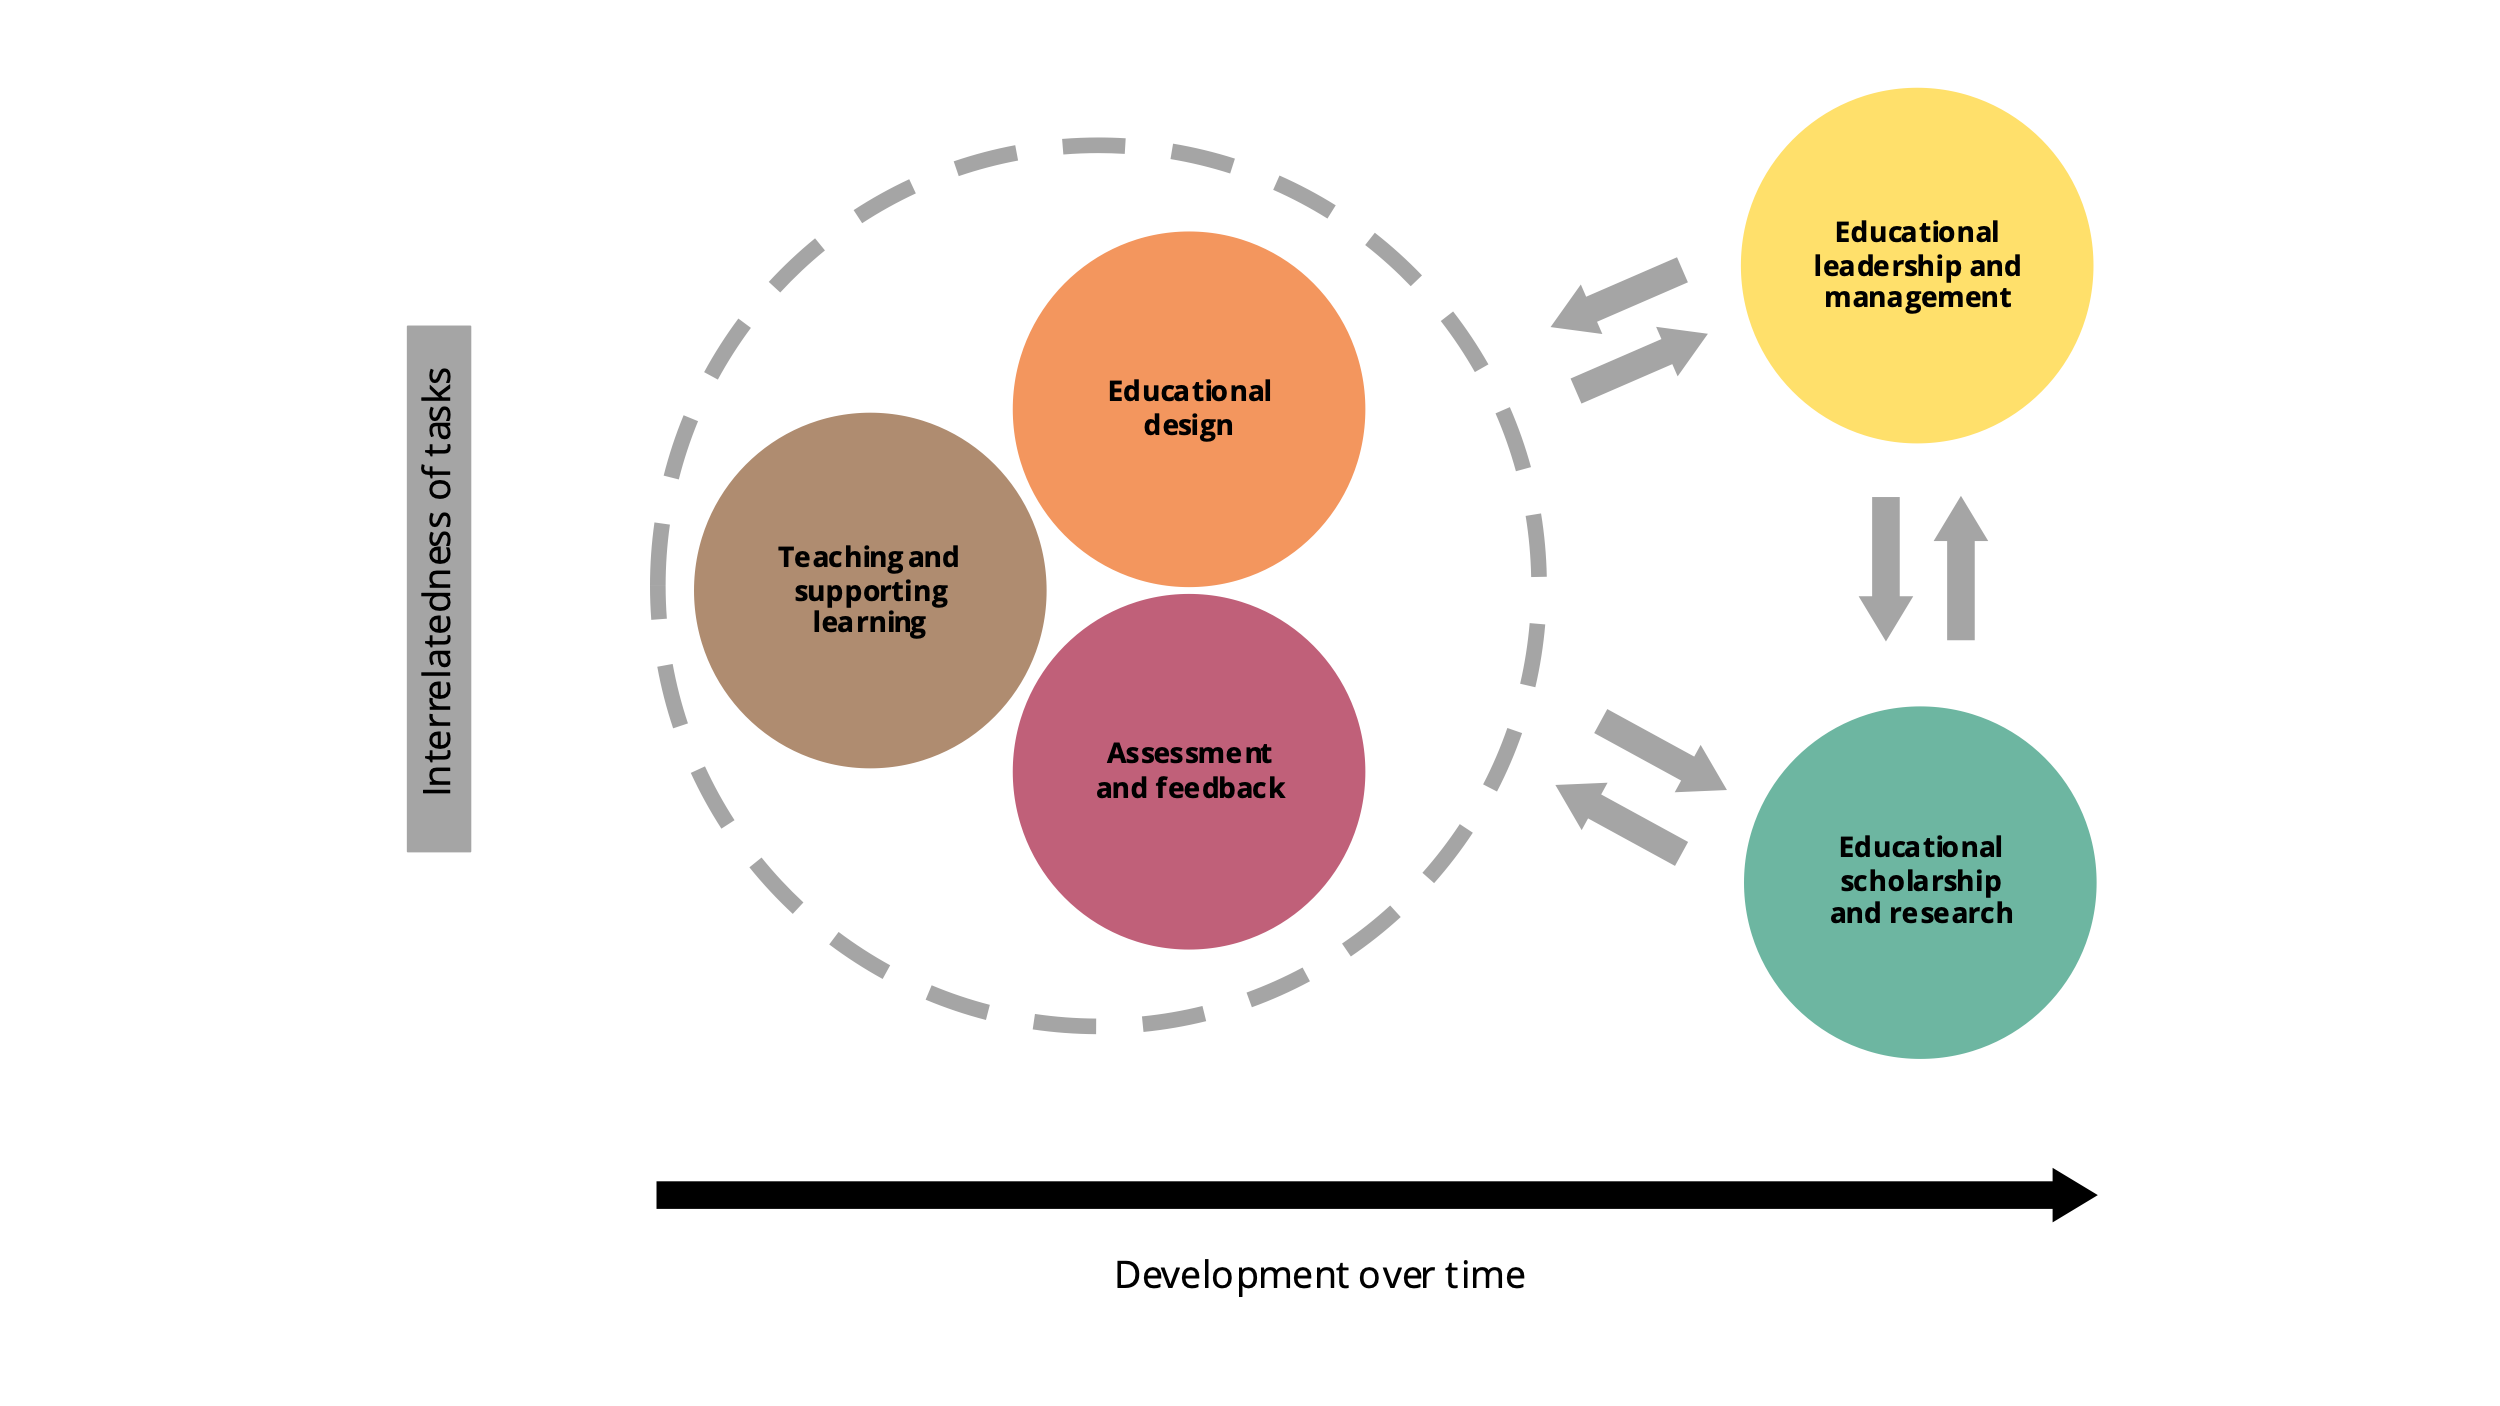
\includegraphics[width=\linewidth]{media/image9.png}



		\label{fig:rId24}



		\caption{Visualisatie van tijd en inhoudelijke relaties tussen verschillende docenttaken van een academicus. Gebaseerd op ‘Academics' expertise development in teacher tasks: A multiple case study'. Van Dijk EE, van Tartwijk J, van der Schaaf MF, Kluijtmans, M. (2023). (onder review voor publicatie).}
	\end{figure}



	\subsubsection{Van solo naar teamsport}



	Moet nu elke docent onderwijskundig leider worden, of leren om onderzoek naar diens eigen onderwijs uit te voeren. Nee, dat zou een enorme verdunning van aandacht en mankracht betekenen, als elke academicus zich continu op alle fronten expert moet tonen. Cruciaal is om te denken en werken in teams. Academici, maar ook diverse type experts en ervaringsdeskundigen met verschillende unieke profielen, kunnen elkaar aanvullen en versterken. Voor elke vakgroep zou gewenst zijn dat er binnen de geledingen een of meerdere academici zijn met een expertiseaccent in onderwijs. Deze \emph{scholarly}\emph{ }\emph{teachers} die kennis over onderwijs kunnen toevoegen aan het team en kennis kunnen generen voor de continue ontwikkeling en optimalisatie van onderwijs in het betreffende veld.



	Deze onderwijsspecialisten onder de academici, die we hier zullen duiden als \emph{scholarly} docenten vormen namelijk de cruciale link tussen beleid, innovatie en uitvoering. Zij kunnen het onderwijs voortdurend aanpassen om studenten up-to-date onderwijs van de hoogste kwaliteit te bieden. Bijvoorbeeld een docent die zich toelegt op het bevorderen van inclusiviteit\index{inclusiviteit} van een opleiding, hiernaar onderzoek doet en interventies ontwikkelt. Deze docent verbetert niet alleen de eigen opleiding en implementeert hiermee beleid, maar door het onderzoek worden de inzichten ook breder gedeeld. Vaak zullen we zien dat een dergelijke gevorderde docent als expert gevraagd wordt om mee te denken over verdere ontwikkeling van beleid in het eigen instituut of daarbuiten, of als spreker op een congres. We zien hier dus een heel sterke wisselwerking tussen beleid, onderzoek en onderwijs. Wanneer docenten bijdragen aan kennis over het eigen onderwijs door context-specifieke inzichten te genereren en deze te delen met collega's, wordt dit ook wel \emph{Scholarship\index{scholarship} of Teaching and Learning} (SoTL) genoemd. Het doel van SoTL is om de praktijk in de eigen klas het leren van studenten te verbeteren binnen een (reeks) disciplinaire cursus(sen). Wanneer het doel van het onderzoek breder is en meer gericht op kennis die ook buiten het eigen onderwijs relevant is spreken we ook wel van ‘discipline-based education research', oftwel onderzoek van onderwijs in de eigen discipline.



	\subsubsection{Samenwerking over faculteiten}



	In een brede onderzoeksuniversiteit is er sprake van onbenut potentieel: Juist de huidige noodzaak tot brede, interdisciplinaire perspectieven kan brede onderzoeksuniversiteiten in hun kracht zetten. De verwevenheid van onderzoek en onderwijs dreigde verloren te gaan in de afgelopen periode maar ligt nu weer onder handbereik. Hierin is een rol weggelegd voor primair disciplinair georiënteerde programma's, waar inter- en transdisciplinaire elementen zorgen voor een verdieping op de eigen discipline en het stimuleren van vaardigheden en een attitude die nodig zijn voor samenwerking. Maar er is eveneens ruimte voor brede interdisciplinaire bachelor- of masterprogramma's, zoals \emph{liberal}\emph{ arts}\emph{ \& }\emph{sciences} programma's of colleges waar interdisciplinariteit centraal staat en de student opgeleid wordt om tot integratie van inzichten te komen. Hun unieke plaats in het stelsel is om mensen op te leiden voor wie de brede blik bij uitstek voorop staat in hun leren en denken, maar die ook allen op een of meerdere disciplines dusdanig de diepte in gaan dat zij een unieke bijdrage ontwikkelen in hun rol on onderzoek of maatschappij. De aanwezigheid van een brede range van disciplines aan een universiteit biedt dus een enorm potentieel, waarbij er sprake kan zijn van een herwaardering van een divers palet aan onderzoeksculturen en perspectieven, en studenten daar in hun opleiding ook echt mee in aanraking komen. Dit soort potentieel komt niet spontaan tot zijn recht maar vereist veranderingen in organisatie en cultuur.



	\section{Het stelsel}



	Het aantal universitaire studenten neemt al decennia toe. Dit leidt tot problemen op stelselwijze. Hoe zien we dit idealiter voor ons in de toekomst? Bekostiging voor studenten zou nominaal gelijk moeten blijven en zowel een onderwijs- als onderzoekscomponent moeten kennen zodat hoger onderwijs altijd die samenhang als basis heeft. De vraag is ook of de studenten allemaal op de juiste plek terecht komen. Het is een goede zaak iedereen gelijke kansen te bieden. Hiertoe moet betaalbaarheid van het hoger onderwijs in de gaten worden gehouden. Beurzen, ooit ingevoerd voor vergroten kansengelijkheid en toegankelijkheid, zijn een leenstelsel geworden met voor sommigen hoge studieschulden als gevolg.\footnote{Comijs et al., ‘Opkomst en Ondergang'.} Een beperkte vorm van basisbeurs keert momenteel terug, maar studeren vraagt om een forse investering. De hoge kosten kunnen drempels opwerpen voor participatie in het hoger onderwijs. Bovendien treffen de uiteindelijke studieschulden juist degenen die kwetsbaar zijn, die door slechte fysieke of psychische gezondheid deze schulden na afloop niet makkelijk kunnen terugbetalen. Vanuit een open visie op onderwijs moeten we toegankelijkheid en betaalbaarheid dus goed bewaken.



	Als we spreken over toegankelijkheid willen we daarmee niet stellen dat iedereen hoger onderwijs moet volgen. Integendeel. Lager- en middelbaar beroepsonderwijs wordt vaak ondergewaardeerd want is essentieel voor het opleiden van vaklieden die hard nodig zijn in de maatschappij. De enorme stroom naar het universitair onderwijs heeft te maken met status en verdienverwachtingen, al dan niet reëel. Belangrijk is dus niet om iedereen naar het hoger onderwijs te krijgen, maar wel om iedereen op de juiste plek te krijgen. Het hoger onderwijs zou toegankelijk moeten zijn voor diegenen met het benodigde talent en de benodigde ambitie.



	Bijzonder in Nederland is bovendien ook nog het duale stelsel met HBO\index{hoger beroeps onderwijs (HBO)} en WO\index{wetenschappelijk onderwijs (WO)}. Hoewel beide hoger onderwijs is, wordt aan het wetenschappelijk onderwijs\index{wetenschappelijk onderwijs (WO)} veelal een hogere status toegekend dan aan hoger beroepsonderwijs. De term universiteit wordt in Nederland vooral aan wetenschappelijk onderwijs\index{wetenschappelijk onderwijs (WO)} gekoppeld, terwijl in Engelstalige landen voor beide vormen van onderwijs de term \emph{university} wordt gebruikt. We zien in Nederland een voortschrijdende verschuiving van HBO\index{hoger beroeps onderwijs (HBO)} naar universitair. Het risico is echter dat we tekorten zien in hoger opgeleiden met een professionele focus, en dat voor het academische onderwijs het academische karakter verdwijnt, zowel door ontstane tekort aan financiering\index{financiering}, als door de instroom van studenten zonder de gewenste wetenschappelijke nieuwsgierigheid of capaciteiten. Studenten die beter op hun plek zouden zijn geweest in HBO-onderwijs maar door druk van zichzelf, familie of \emph{peers} kiezen voor de universiteit. Extrinsieke in plaats van intrinsieke motivatie. Voor het goed opleiden van de student van de toekomst is het wenselijk de statusverschillen binnen het hoger onderwijs te verkleinen en het accent echt op de aard en inhoud van de studies te focussen. Alleen dan kan iedereen talent goed ontwikkelen en kunnen we zowel de academici als professionals opleiden die de maatschappij nodig heeft.



	Hoewel uitwisseling tussen universiteiten van alle tijden is, was dit in het verleden vooral via individuele mobiliteit van staf en studenten. De geglobaliseerde wereld, met de complexe problemen waarvoor we ons gesteld zien, brengt een noodzaak met zich mee als collectief kennissysteem te werken. Alleen dan kunnen we de complexe problemen snel adresseren. COVID-19\index{COVID-19} heeft mooi gedemonstreerd dat als wetenschappers wereldwijd kunnen samenwerken we daarmee ongekend snel inzichten en toepassingen kunnen bereiken. Tegelijk zagen we ook aan het ontstaansrisico van virussen, evenals aan antivaccinatie bewegingen en verschillen in vaccinatiegraad en pandemie aanpak dat zelfs een virale pandemie net zozeer een sociaal cultureel als biomedisch probleem is. Dit alles vraagt om samenwerking, niet alleen tussen disciplines zoals hierboven al geschetst, maar ook geopolitiek. Wat betekent dit voor het opleiden van nieuwe generaties en ons ontwikkelingsaanbod voor de huidige generatie? We moeten van individuele programma's aan individuele hoger-onderwijsinstellingen, veel meer naar opleiden in netwerken en allianties. Naast flexibiliteit voor de individuele student zoals hierboven al beschreven, moeten we ook moeten krachten bundelen organisatorisch en strategisch, op institutioneel en stelsel niveau. Dergelijke institutionele samenwerkingen kunnen uiteraard niet zonder (digitale) staf en student mobiliteit, maar anders dan voorheen moet veel meer structureel en hybride worden. Denk aan cursussen en programma's die in samenwerking over instituten geprogrammeerd en aangeboden worden. Aan virtuele internationale classrooms, of virtuele docentschappen waardoor experts hun expertise bij meerdere samenwerkende instituten kunnen inzetten. Sociale interactie is een cruciaal element in leren en kenniscreatie, dus dit betekent zeker niet alles online, maar juist door met structurele partnerschappen te werken zal de fysieke reis versus online-samenwerking verhouding flink kunnen verschuiven naar dat laatste. Als je elkaar eenmaal kent is online samenwerking makkelijker en effectiever. Bewuste keuze dus tussen reizen en online voor samenwerking.



	Voor het stelsel betekent dit grote veranderingen. Binnen onze instituten moeten we ons heroriënteren op de facultaire indeling. Hoewel de disciplinaire band onverminderd van belang is en blijft, zijn de financiële en organisatorische inrichting nu dusdanig sterk facultair gericht dat samenwerking over facultaire grenzen in onderwijs enorm belemmerd wordt. Geldstromen zouden bijvoorbeeld gekoppeld kunnen worden aan de student in plaats van aan de programma's waardoor zowel keuzevrijheid als uitwisseling of samenwerking in onderwijs over faculteiten heen veel makkelijker te organiseren wordt.



	Landelijk en zeker internationaal moet wet- en regelgeving aangepast worden om inter-institutionele samenwerking in onderwijs te faciliteren.



	Ook kwaliteitszorg, moet interfacultaire, inter-institutionele en internationale programma's gaan faciliteren, evenals het onderwijs voor professionals\index{onderwijs voor professionals}. Hiertoe moet deze anders ingericht gaan worden. Elk land heeft nu zijn eigen accreditatiesysteem. Erkenning van elkaars accreditatie en/of inrichting van accreditatie op Europees niveau is nodig. En een systeem van ‘\emph{micro-}\emph{credentialing}' kan modulaire aanbod academische kwaliteitsbewaking en status verlenen, wat kan helpen bij flexibilisering van bachelor-, master- en PhD programma's, maar zeker cruciaal is voor het onderwijs voor professionals\index{onderwijs voor professionals}.



	Binnen Europa zien we dat met de ‘European Universities', een initiatief en fonds van de Europese commissie, een enorme beweging op gang is gebracht om intensiever over de grenzen van instituten en landen heen samen te werken. Een voorbeeld wordt gegeven in Tekstbox 3 - 7, de CHARM-EU alliantie. Dit is slechts één van de 41 allianties die de EU in 2022 kent. Deze intensivering van Europese samenwerking is nodig om ons op lange termijn goed te verhouden tot de Amerikaanse en Aziatische universiteiten. Door samen op te trekken en elkaar te versterken kunnen de Europese universiteiten gezamenlijk de goede reputatie en kwaliteit op gebied van academische opleidingen handhaven op langere termijn. Dat wil niet zeggen dat we niet ook buiten Europa moeten samenwerken, maar de samenwerking binnen Europa dient veel meer stelselmatig te zijn, daarbuiten meer op inhoud gericht.

	\enlargethispage{\baselineskip}\checkandfixthelayout\enlargethispage{\baselineskip}\checkandfixthelayout\enlargethispage{\baselineskip}\checkandfixthelayout
	\begin{bookbox}{\raggedright tekstbox 3 - 7. \\charm-eu, een european university programma.}
		CHARM-EU is een door de EU, via het Erasmus+ programma, gefinancierd initiatief met als doel structurele en strategische samenwerking tussen Europese universiteiten. Acht Europese instellingen maken deel uit van CHARM-EU, waaronder de Universiteit Utrecht.

		\vspace*{\baselineskip}

		CHARM-EU vertegenwoordigt een \emph{CH}\emph{allenge-driven}, \emph{A}\emph{ccessible}, \emph{R}\emph{esearch-}\emph{based}, en \emph{M}\emph{obile} model voor de co-creatie van een Europese universiteit in lijn met de Europese waarden en de \emph{Sustainable}\emph{ Development Goals}.

		\vspace*{\baselineskip}

		In september 2021 lanceerde CHARM-EU een masteropleiding: MSc in \emph{Global }\emph{Challenges}\emph{ }\emph{for}\emph{ }\emph{Sustainability}. Centraal staan mondiale uitdagingen op het gebied van duurzaamheid. De masteropleiding biedt een uniek internationaal programma. Studenten gaan aan de slag met duurzaamheidsvraagstukken in een transdisciplinaire omgeving, gebaseerd op concrete maatschappelijke uitdagingen.

		\vspace*{\baselineskip}

		Naast het masterprogramma is er ook een CHARM-EU transdisciplinair\index{transdisciplinair} onderzoeksinitiatief: \href{https://www.charm-eu.eu/torch}{TORCH} (\emph{Transforming}\emph{ Open }\emph{Responsible}\emph{ Research }\emph{and}\emph{ }\emph{Innovation}\emph{ }\emph{through}\emph{ CHARM}). TORCH heeft tot doel een gemeenschappelijke agenda voor onderzoek en innovatie te ontwikkelen.
	\end{bookbox}\enlargethispage{\baselineskip}\checkandfixthelayout

	\section{Slotbeschouwing}



	Een laatste reflectie betreft het belang van publieke opinie en maatschappelijk draagvlak. Hierin zijn er parallellen met public engagement\index{public engagement} zoals in het hoofdstuk over \emph{Open }\emph{Science} is beschreven. ‘\emph{Public engagement\index{public engagement}}' waarbij de universiteit interacteert met een breed publiek draagt bij aan het publieke debat, aan impact en aan draagvlak. Dit is van groot belang voor de bereidheid van maatschappelijk partners om samen te werken in onderzoek en onderwijs, voor het baseren van publieke en politieke besluiten op wetenschappelijke kennis, en ook voor de wet- en regelgeving en financiering\index{financiering} van ons onderwijs. We grijpen als voorbeeld even terug op een voorbeeld wat al aan de orde is geweest: het punt van zorg over het gebrek aan draagvlak voor internationalisering\index{internationalisering} van universiteiten. Vanuit universitair perspectief, gestaafd met onderzoek, zien we internationalisering\index{internationalisering} als cruciaal voor de kwaliteit van onderzoek, onderwijs en maatschappelijke impact. Willen we als universiteiten onze internationale instroom van staf en studenten behouden of zelfs uitbouwen, zullen we de noodzaak daartoe veel duidelijker moeten maken aan de politiek en het publiek. Integraal deel van onze maatschappelijke missie is dan ook het uitdragen van wat we doen, waartoe de universiteit op aarde is. We willen meerwaarde te creëren in onze interactie met de maatschappij. Alleen door deze meerwaarde ook helder over voetlicht te brengen, kunnen we de maatschappelijke belofte van onderzoek en onderwijs ook daadwerkelijk realiseren.







	\chapter{Community }



	\section{De universiteit, dat zijn haar mensen }



	Een universiteit bestaat eerst en vooral uit haar mensen. Natuurlijk kent een universiteit ook organisatorische en fysieke aspecten: met haar gebouwen, productie, geldstromen, kaders en regels. Maar toch is een universiteit in essentie een abstracte en levende entiteit die gevormd wordt door haar gemeenschap\index{gemeenschap}. De cultuur in die gemeenschap\index{gemeenschap}, die zich zowel uit in de omgang met elkaar als met de buitenwereld, is waarde-gedragen. Publieke waarden waar we elkaar op willen aanspreken zijn wetenschappelijke en persoonlijke integriteit, inclusiviteit\index{inclusiviteit}, en maatschappelijk betrokkenheid, zoals ook in de andere hoofdstukken aan de orde is gekomen. Acterend vanuit deze grondwaarden wordt kennis gemaakt, gedeeld en toepast, en worden de voorwaarden geschapen waarbinnen deze primaire processen kunnen plaatsvinden. Dit gebeurt in een ideale universitaire gemeenschap\index{gemeenschap} vanuit teamgeest gedreven complementaire samenwerking met anderen. De gemeenschap\index{gemeenschap} wordt gevormd door iedereen die bezoldigd dan wel onbezoldigd deel uitmaakt van de universiteit en haar netwerk. Dat zijn dus niet alleen de academische en niet-academische staf, maar ook de studenten, (inter)nationale collega's, en derden zoals maatschappelijke partners met wie (langdurige) functionele contacten bestaan. Hoe al deze mensen met elkaar en met hun werkzaamheden omgaan, bepaalt zowel het karakter als de wetenschappelijke en maatschappelijke impact van de universiteit.



	In dit hoofdstuk zoomen we daarom in op de community als het hart van de universiteit. Naar we hopen een warm kloppend hart, waar mensen zich gezien en gehoord voelen en graag deel van uitmaken. Maar helaas is de realiteit soms anders. De academische gemeenschap\index{gemeenschap} knarst en kraakt momenteel. De werkdruk is veelal onacceptabel hoog, de onzekerheid groot, er is vaak ongezonde competitie en de teamgeest is lang niet altijd aanwezig. De veelheid van korte, losse arbeidsrelaties ondermijnt een sterk gevoel van verbondenheid met de universiteit en haar gemeenschap\index{gemeenschap}. Zo zijn er veel tijdelijke docenten zonder academisch toekomstperspectief. Bovendien ondermijnen regeldruk, protocollen en verantwoording de intrinsieke motivatie om deel uit te maken van een waardengemeenschap waar gezamenlijk aan kennisproductie en deling gewerkt wordt. Mensen vertrekken om deze redenen, zoals beeldend verwoord is door Eelco Runia in zijn boek ‘Genade zesjes'.\footnote{Runia, \emph{Genadezesjes}\emph{.}} Het uit zich ook in bewegingen zoals ‘WO\index{wetenschappelijk onderwijs (WO)} in actie', een door diverse universiteiten ondersteund landelijk platform dat opkomt voor de belangen van het universitair onderwijs. En dat pleit voor versterking van verwevenheid van onderwijs met wetenschappelijk onderzoek. Deze verwevenheid is door forse, langdurige bezuinigingen en een snelle toename van het aantal studenten onder grote druk komen te staan.\footnote{\href{https://woinactie.blogspot.com/p/over-wo-in-actie.html}{https://woinactie.blogspot.com/p/over-wo-in-actie.html}, geraadpleegd 2 januari 2023.} De kritiek is een duidelijk signaal met name vanuit wetenschappelijk personeelsperspectief. Daarnaast zijn er ook andere problemen, zo wordt een grote kloof ervaren tussen wetenschappelijk en ondersteunend personeel. Eerder gegeven oplossingsrichtingen zijn veelal beperkt, geven weinig richting over hoe we meer vanuit teams kunnen opereren en duidelijker antwoord kunnen geven als universiteit op uitdagingen en verwachtingen vanuit de maatschappij. Een dergelijke verandervisie wordt wel gegeven door de systeemanalyse van \emph{Science}\emph{ in }\emph{Transition} (2013, 2014) zoals in het hoofdstuk over onderzoek uitgebreid is besproken. In dit hoofdstuk trekken we die visie verder door naar de implicaties voor community.



	Naast reeds genoemde problemen met werkdruk en de ontstane kloof tussen onderwijs en onderzoek, valt er ook aan inclusiviteit\index{inclusiviteit} en een veilige werkomgeving nog veel te winnen. Een veelheid aan rapporten geven indringende signalen van de universiteit als een onveilige plek, variërend van seksuele intimidatie onder studenten en medewerkers\footnote{Bondestam et al., ‘Sexual Harassment', 397-419.}, tot roddelen, vernederen, achterhouden van informatie en machtsmisbruik.\footnote{FNV/VAWO, \emph{Rapport Sociale veiligheid}. } Voedingsbodems lijken het competitieve klimaat, de hoge werkdruk, en de hoge mate van afhankelijkheidsrelaties. Academische hiërarchie is een fundamenteel onderdeel van een universitair systeem maar kan leiden tot ongewenste machtsrelaties. Een commissie met als voorzitter Naomi Ellemers schreef in 2022 het KNAW-rapport ‘Sociale veiligheid in de Nederlandse wetenschap, van papier naar praktijk'.\footnote{KNAW, \emph{Rapport Sociale veiligheid}.} Niet alleen wordt daarin inzichtelijk gemaakt dat er werk gemaakt moet worden van sociale veiligheid, maar ook dat dit wetenschappelijk integriteit ten goede komt en andersom. Goede wetenschap en sociale veiligheid versterken elkaar. Beide komen niet vanzelf en voor beide aspecten moet daarom bewust en expliciet aandacht zijn. We moeten met elkaar ook de moeilijke dingen kunnen en durven benoemen, en het ongemak dat daarmee gepaard gaat omarmen.



	We zullen in dit hoofdstuk beschrijven hoe we een open, inclusieve, sociaal veilige, en tegelijk intellectueel uitdagende omgeving voor ons zien. Een omgeving waar mensen zich welkom en gehoord voelen, uitgedaagd worden het beste uit zichzelf te halen, waar luisterend en respectvol met een veelheid aan meningen, achtergronden, inzichten en perspectieven wordt omgegaan, en waar het een sine qua non is om je in te zetten voor de mensen om je heen en de maatschappij. We zullen daarbij ook ingaan op drempels, uitdagingen en risico's. Want waar mensen samenkomen, is nooit alleen maar harmonie: zoveel zielen zoveel gedachten en wensen. Maar zoals in voorgaande paragraaf is geschetst is er momenteel meer aan de hand dan alleen een verscheidenheid aan meningen en is er sprake van ongelijkheid en onveiligheid. Idealiter wordt de veelheid aan gedachtes en meningen juist de kracht van de universiteit, waar vele stemmen worden gehoord en het academisch debat niet geschuwd wordt: want vanuit diversiteit\index{diversiteit} komt kwaliteit. We realiseren ons dat we niet direct een praktisch antwoord bieden op de huidige problemen. Maar door een wenkend perspectief te schetsen hopen we wel een richting te geven bij het zoeken naar antwoorden.



	\section{Van individu naar teams}



	Zoals eerder gezegd, zien we de universiteit idealiter als een bloeiende gemeenschap\index{gemeenschap} gericht op genereren, toepassen en delen van kennis voor de maatschappij. Een lerende gemeenschap\index{gemeenschap}, die open staat voor leren van en met elkaar. Leren door nieuwe kennis te genereren in onderzoek, leren door deze kennis toe te passen, leren door kennis te delen in onderwijs. De term lerende gemeenschap\index{gemeenschap} is niet nieuw, en werd al genoemd in het klassieke Von Humboldtse model waar de universiteiten van nu op gebaseerd zijn. In Von Humboldts model betrof de lerende gemeenschap\index{gemeenschap} echter een gesloten academische gemeenschap\index{gemeenschap}, die bovendien sterk gericht was op individuele interactie en prestatie. Noch het gesloten, noch het individuele karakter zijn in onze ogen nog langer houdbaar. De visie waarvan dit boek doordrenkt is, behelst openheid en teamspirit. We stellen dus een fundamentele verandering voor. De lerende community van de toekomst, waartoe nu al stappen worden gezet, bestaat uit een dynamische en flexibele configuratie van teams. Excellentie wordt niet langer gedefinieerd als de mate waarin een individu presteert, maar als de mate waarin iemand bijdraagt aan succes van verschillende teams. Dit betekent naast inhoudelijk presteren ook een nadruk op leiderschap en het creëren van een open cultuur waarin mensen elkaar met respect voor andere meningen kunnen en durven aanspreken. De maatschappij is sterk veranderd en de uitdagingen zijn immens. Zoals in voorgaande hoofdstukken is bepleit, zal het wetenschappelijk werk in onderzoek en onderwijs veel minder individueel worden en zijn teams onontbeerlijk voor het doceren, onderzoeken en aanpakken van complexe problemen in de moderne digitale mondiale maatschappij. In onderzoek, onderwijs, en ook in de organisatie van de universiteit hebben we met deze complexiteit te maken. Het oude idee van de geniale eenling was ook voorheen al een mythe, niemand presteert ooit geheel alleen, maar topprestaties werden voorheen wel vaak aan individuen toegeschreven.



	In de toekomst zal echt nog sterker dan in het verleden gelden dat topprestaties alleen in teams bereikt kunnen worden. Naast het verschuiven van de focus van individuele naar teamprestatie, brengt ons dat op een tweede belangrijk uitgangspunt van de lerende gemeenschap\index{gemeenschap}: diversiteit\index{diversiteit}. Diversiteit\index{diversiteit} is vanuit het oogpunt van complementariteit in teams geen luxe maar noodzaak. Neem bijvoorbeeld onderwijs. In onderwijs zijn samenwerking en wisselwerking tussen docenten, studenten en stakeholders onmisbaar, evenals de samenwerking met didactische en informatietechnologie experts. Maar vergeet ook het brede palet aan organisatieaspecten niet: van campusinrichting tot zaalbeheer, van studentadministratie tot surveillant, van beleid tot kwaliteitszorg. Voor al deze aspecten zijn mensen verantwoordelijk en deze actoren staan niet los van elkaar, maar interacteren. Een keten is zo sterk als de zwakste schakel. Als samenwerking constructief is, wordt het geheel meer dan de som der delen en levert synergie op. Samenwerking kan echter haperen, bijvoorbeeld door een gebrek aan aanspreekcultuur of juist intolerantie en het ‘cancellen' van bepaalde visies en sociale onveiligheid. Dan worden zwakke schakels in een proces niet altijd gesignaleerd of aangepakt, met het risico van suboptimaal of zelfs disfunctioneren van een team.



	We realiseren ons terdege dat samenwerking niet altijd makkelijk is. Samenwerking kan alleen slagen als er sprake is van gezamenlijke doelen en ambitie, tolerantie, acceptatie en zowel persoonlijk als organisatorische flexibiliteit. Waarom loopt het nu vaak spaak? Zoals hiervoor aangeven moeten we in elk geval zorgen voor binding met de organisatie en met elkaar, community dus. Dat vraagt in elk geval om een veilige en inclusieve cultuur, acceptabele werkdruk, waardering van bijdragen aan teams, een heldere missie en visie, en leiderschap. Waarin we steeds open en actief met elkaar verkennen wat goed gaat maar ook wat nog niet goed gaat.



	Wat is een team? Het begrip ‘team' heeft hier een ruime betekenis: als elke constellatie waarin mensen voor korte of langere tijd samenwerken rondom een gezamenlijk doel. Het gezamenlijke doel kan een concrete taak of product zijn, bijvoorbeeld een onderzoeksproject, een cursus of een gehele opleiding. Het gezamenlijk doel kan ook thematisch of abstract zijn, bijvoorbeeld een werkgroep of taskforce rondom een gedeelde interesse, probleem of een ambitie. Kern van een team is dat er iets is wat de mensen samenbrengt en bindt. Teams kunnen dus klein zijn of groot, extern ingesteld of bottom-up ontstaan, losjes gekoppeld of hechte banden kennen, en ze kunnen tijdelijk of structureel zijn. Iedereen zal steeds flexibel en dynamisch deel uitmaken van meerdere teams, en daarbinnen vaak verschillende rollen aannemen. Zie het voorbeeld van de fictieve Laila in Tekstbox 4 - 1.

	\begin{bookbox}{\raggedright tekstbox 4 - 1. \\het voorbeeld van laila en haar teams.}
		Laila heeft recent een vaste aanstelling gekregen als universitair docent. Haar thuisbasis is de leerstoelgroep waar ze onderdeel van uitmaakt. Zij geeft les in een interdisciplinaire bachelor en maakt daarmee zowel deel uit van het docentteam van haar cursus, het brede team van docenten, en ondersteuners van de opleiding, en van de zeer brede onderwijsgemeenschap van het programma (waar naast docenten en ondersteuners ook de studenten, alumni en werkveldvertegenwoordigers deel van uitmaken). Ze is daarnaast betrokken bij een facultair onderwijsinnovatieproject waarin ze samen met centrale en facultaire didactisch en IT-experts een innovatieteam vormt. Vanuit haar onderzoekstaken maakt ze deel uit van een leerstoelgroep, welke samen met andere leerstoelgroepen een bredere disciplinegroep vormt. Ze is lid van een projectteam van een onderzoekconsortium met een tweetal internationale universiteiten en een industriële partner. Ze maakt als begeleider van een promovendus deel uit van een promotieteam, en in breder verband van de \emph{graduate}\emph{ school}. Vanuit haar betrokkenheid bij de universiteit en de maatschappij is ze lid van een facultaire adviescommissie over diversiteit\index{diversiteit}. Ook maakt ze deel uit van een team vrijwilligers die op zaterdag lesgeven in de weekendschool om kansengelijkheid te bevorderen. Ze schrijft in haar vrije tijd een boek waarvoor ze met een veelheid van mensen spreekt, laat tegenlezen, en laat redigeren. In haar dankwoord bedankt ze dit losjes-gekoppelde ‘team' van meedenkers...
	\end{bookbox}

	Het fictieve voorbeeld illustreert dat iemand zelden onderdeel uitmaakt van slechts één team, en al snel in meerdere teamverbanden opereert. Soms staan deze teams naast elkaar, soms zijn het kleinere teams binnen grotere of bredere teams, soms is er sprake van gedeeltelijk overlappende teams. We hadden hier andere voorbeelden kunnen gebruiken, zowel academisch als niet academisch. Iedereen die zijn eigen agenda raadpleegt zal waarschijnlijk meerdere ‘teams' kunnen identificeren, van eenmalige of kortdurende samenwerkingsverbanden tot structurele of langdurige samenwerkingsverbanden. In de praktijk gebruiken we niet voor elk samenwerkingsverband de term team, maar teamwork is wel de basis voor alles wat we doen, of het nu de kantine beheren is, een onderzoeksproject uitvoeren of een afdeling runnen.



	Wat belangrijk is, juist in deze veelheid van teams, is dat iedereen een thuisbasis heeft. Een thuisbasis in de vorm van een of meerdere teams die een structurele basis geven, zowel organisatorisch als sociaal. Die vanuit een formele structuur zorg dragen voor de coaching en begeleiding van een individu in de veelheid van teams, en daarmee ook zorgen voor het gevoel van een thuisbasis. Een plek waar je je bij voelt horen en waar je gekend en gezien wordt. Een leidinggevende moet nadrukkelijk oog hebben voor de veelheid van teams, coachen in de keuzes en prioritering daarin, en prestaties over het geheel aan werk-gerelateerd teams meenemen in beoordeling. Een vaak onderbelicht aspect hiervan is ook het waarderen van inspanningen om te verbinden: om eigen kennis, ervaring en expertise vanuit verschillende teams te verbinden (\emph{boundary}\emph{ }\emph{spanning}), of om expertise van anderen met elkaar te verbinden (\emph{brokering}). Dit soort grens-overbruggende werkzaamheden zijn cruciaal voor een goed functionerende teamstructuur, zowel binnen een team als tussen teams. De verbindingsactiviteiten dragen vaak niet rechtstreeks of zichtbaar bij aan prestaties maar zijn het onmisbare bedradingscircuit zoals van een auto, wat zorgt dat de verschillende onderdelen samenwerken om tot optimale rijprestaties te komen. Stel je eens voor dat je vier prachtige wielen hebt, een soepel lopende motor, een chauffeur, een stuur, maar dat deze niet met elkaar verbonden zijn…. Misschien een te simpel voorbeeld? Toch zien we dit in de praktijk soms gebeuren. Dat mensen zo hard werken om hun specifieke onderdeel te laten draaien, hun ‘eigen' taak op orde hebben, dat ze het grotere geheel uit het oog verliezen, en daar ook niet op afgerekend of aangesproken worden. Dit heeft het risico dat inspanningen die nodig zijn om eigen handelen goed te coördineren met andere activiteiten, om anderen te helpen, en om op de eigen taak te reflecteren en indien nodig transformeren, minder gezien en daarmee ook minder gewaardeerd of aangemoedigd worden. Daar is het huidige systeem niet goed op ingericht. In de volgende paragrafen gaan we hier verder op in want beter waarderen van deze teamwork-gerichte attitude en inspanningen is fundamenteel voor het realiseren van de open cultuuromslag.



	Voor een individu betekent deze visie dat deze zich zowel bewust moet zijn van zichzelf als van diens omgevingen en de interactie daarmee. In andere woorden: van de context en rol waarin diegene zich op een bepaald moment bevindt. Iemand moet diens eigen kwaliteiten kennen en de grenzen daarvan, en hoe deze kunnen bijdragen in de verschillende omgevingen. Voorwaardelijk is ook om het nut en noodzaak in te zien om zowel inzichten, producten en mensen uit verschillende omgevingen te verbinden. Dat vereist een houding waarin verantwoordelijkheid niet wordt afgeschoven door naar anderen te kijken of te wijzen, maar waarin iemand zich continu afvraagt ‘Wat kan ik doen om anderen c.q. de verschillende teams goed te laten functioneren'. En daarbij hoort ook ‘Wat moet ik niet doen, want kunnen anderen het beter of waar kan ik iemand kansen bieden'. Dit vereist een open, verantwoordelijk en betrokken houding, waarbij iemand het team plaatst voor het eigenbelang. Het vereist naast houding ook kennis en vaardigheden voor het werken met anderen of over disciplinaire en sociaal culturele grenzen geen.



	Zoals in de voorgaande paragraaf geschetst is, betekent dat ook dat ‘verbindings-activiteiten' gewaardeerd moeten worden, naast directe resultaatbijdragen. Om recht te doen aan de veelheid van teams zal in aansturing brede feedback\index{feedback, feed-up, feedforward} over en uit de veelheid van teams waarbinnen iemand functioneert moeten worden meegenomen. Een vorm van afdelingsstructuur en een leidinggevende blijft nodig, maar dit krijgt een andere functie dan voorheen namelijk het borgen van een thuisbasis. Het huidige, in principe eendimensionale model zal namelijk op zichzelf nooit recht kunnen doen aan de veelheid van functies en rollen in teams. Een leidinggevende zal meer en meer in erkenning, waardering en ontwikkeling van medewerkers over de grenzen van een thuisbasis heen moeten kijken. De leidinggevende krijgt dus veel meer een coachende rol dan een aansturende rol, en kijkt vanuit een breed organisatie perspectief naar iemands functioneren en ontwikkeling. Deze nieuwe coachend leidinggevende structuur en cultuur moet worden ontwikkeld, maar er zijn al wel voorbeelden te geven van instrumenten die ten dienste zouden kunnen staan van deze visie. Dat betreft bijvoorbeeld een brede vlootschouw. Hierin beschouwen leidinggevende gezamenlijk hoe medewerkers functioneren en waar hun talenten liggen, met als doel te kijken hoe ieders talenten optimaal ingezet en ontwikkeld kunnen worden. Een dergelijk team-gerichte aanpak kan mobiliteit faciliteren en input geven voor een proactief talentbeleid. Het kan ook zorgen voor optimale invulling van de diverse rollen in teams. Medewerkers moeten bij mobiliteit en ontwikkeling uiteraard zelf een belangrijke stem hebben, en input kunnen geven voor of in de schouw. Maar het voordeel bij een brede vlootschouw is dat een individu veel minder afhankelijk is van diens leidinggevende of eventueel persoonlijke contacten buiten de eigen afdeling, maar standaard breed wordt gezien door de organisatie.



	Bovenstaande teamgericht werken en denken geldt onverkort voor iedereen in de universitaire gemeenschap\index{gemeenschap}. Als we hierbinnen toch even inzoomen op de academische taken dan zijn er in elk geval twee kerntaken te onderscheiden: onderzoek en onderwijs. Zoals reeds eerder bepleit kenmerkt de verwevenheid van onderzoek met onderwijs het universitaire onderwijs. Maar ook de verwevenheid met toepassing van die kennis in professionele rollen, zoals bijvoorbeeld klinisch werk, en toegepaste rollen in het bedrijfs- of maatschappelijk leven, is uiterst relevant. Vandaar dat public engagement\index{public engagement}, maatschappelijke impact en professional performance expliciet wordt benoemd, denk bijvoorbeeld aan klinische werkzaamheden van academici in een academisch ziekenhuis die uiterst relevant zijn voor hun onderzoeks- en onderwijsactiviteiten. Eerder hebben we ook al het belang van teaminzet via verbindingsactiviteiten genoemd, en in andere hoofdstukken benadrukten we reeds het belang van impact en leiderschap. Maar moet dan iedereen dus alles doen en kunnen, en daarin dan bovendien ook nog leadershap tonen om carrière te maken? Het antwoord is daarop een heel duidelijk: nee. Wat van fundamentele en cruciaal belang is, is dat iedereen via teams actief verbonden is met zowel onderzoek als onderwijs, en indien relevant professional performance. Maar een individu kan niet en hoeft niet overal en altijd in te excelleren om een uitstekende academicus te zijn.



	Voor onderwijs en onderzoek is er sprake van minimumdrempelwaardes: elke academicus wordt geacht onderwijs te geven en betrokken te zijn bij onderzoek. Voor academici met een accent op onderzoek of impact betekent dit dat zij minimaal hun expertisekennis uitdragen via onderwijs. Voor academici die het accent in hun profiel echter leggen op onderwijs ligt de lat wat betreft onderwijs veel hoger en wordt onderwijskundig leiderschap verwacht. Voor hen geldt juist de drempelwaarde als het gaat om onderzoek. Zij dienen minimaal op de hoogte en betrokken te zijn bij onderzoek dat raakt aan de lesstof die zij doceren. De invulling van zowel de minimumdrempelwaardes als wat als excellent wordt gezien, is deels een politieke en culturele discussie, en wordt in eerste instantie door de lokale context en strategie van de universiteit bepaald. Minimum drempels zullen in elk geval iets moeten zeggen in termen van maximaal tussenliggende tijd of minimum output volume. De belangrijkste leidraad daarbij dient te zijn dat de combinatie inclusief de ondergrenzen, in dienst staan van de kwaliteit van onderwijs en onderzoek: dat iemand doceert vanuit een actieve (team)betrokkenheid in onderzoek, en dan iemand onderzoekt vanuit een actieve (team)betrokkenheid in het uitdragen van de nieuwe kennis. Dat betekent ook dus heel concreet dat men tot de conclusie kan komen dat full time docentschap of full time onderzoek doen ongewenst is, tenzij het nadrukkelijk een fase is in een zich verder ontwikkelende carrière (bijvoorbeeld een of enkele jaren full time focus op onderzoek dan wel onderwijs waarna daarna expliciet weer mogelijkheden komen voor een nieuwe loopbaanstap, een combinatie of alternering), of dat er op andere manier zorg gedragen wordt voor continue voeling met en ontwikkeling in de te doceren discipline. Uitzonderingen kunnen en mogen dus bestaan, waarbij echter steeds twee zaken voorop moeten staan, de (lange termijn) kwaliteit van onderzoek en onderwijs, en het voorkomen van fuik-constructies waarin iemand zich niet verder kan ontwikkelen, inhoudelijk of in diens loopbaan.



	\section{De inclusieve gemeenschap}



	De ideale universitaire community is inclusief is in de breedste zin van het woord. Een gemeenschap\index{gemeenschap} waar iedere medewerker en student welkom is en in opgenomen wordt, ongeacht achtergrond, herkomst, etniciteit, geaardheid, cultuur, geloof, politieke overtuigingen en fysieke beperkingen, en alle andere verschillen die er zoal kunnen zijn tussen mensen. Dit klinkt mooi en weinigen zullen hier in beginsel op tegen zijn. Tegelijk is het nog niet zo makkelijk dit in de praktijk daadwerkelijk te realiseren. Zo kiezen mensen bewust en onbewust snel voor omgang met mensen die op hen lijken. En kan samenwerken in diverse teams best wel eens ongemak veroorzaken. Eenieder kan vanuit een eigen perspectief vaak niet door hebben welke drempels ervaren kunnen worden of welk gedrag als kwetsend kan worden ervaren. Het is dus zaak bewust aandacht te besteden aan het stimuleren van diversiteit\index{diversiteit} en inclusie, en aan het open bespreken van ervaren ongemak of kwetsingen. Diversiteit\index{diversiteit} vereist aandacht bij instroom en aannamebeleid, evenals in de samenstelling van samenwerkingsverbanden. Diversiteit\index{diversiteit} is een middel voor kwaliteit en geen op zichzelf staand doel. Toch zullen voor het realiseren van een diverse community, diversiteit\index{diversiteit} en inclusiviteit\index{inclusiviteit} wel degelijk bewuste en actieve doelen moeten zijn als we de drempels die er bestaan willen slechten. Want met het stimuleren van diversiteit\index{diversiteit} in aannamebeleid en samenstelling van teams zijn we er nog niet. De mensen vanuit de diverse instroom moet ook gelijke kansen krijgen, zich goed kunnen uiten en bewegen, om ook echt de vruchten te plukken van die diversiteit\index{diversiteit}. Daarom verdient inclusiviteit\index{inclusiviteit} de aandacht zodra iemand toetreedt tot de gemeenschap\index{gemeenschap}. Of het nu gaat om een student, medewerker of gast. Een inclusieve gemeenschap\index{gemeenschap} betekent dat er niemand bedoeld of onbedoeld structureel wordt buiten gesloten. Dat verschillen worden gerespecteerd en de waarde daarvan wordt ingezien. Dit vergt bewust reflectie van de gemeenschap\index{gemeenschap} op haar eigen omgangsnormen, en het actief opsporen van bewust en onbewust uitsluitende praktijken en gebruiken. Tolerantie, respect en openheid naar anderen is grondvoorwaarde om constructief met elkaar om te gaan. Nieuwsgierigheid naar de ander in plaats van veroordelen op grond van aannames vooraf. Luisteren in plaats van vertellen. Zoals het mooi geformuleerd is in het UMC Utrecht in haar omgangsnormen: eerst begrijpen en dan pas begrepen worden. Oprechte nieuwsgierigheid en interesse zijn dus essentieel en zijn tevens de basis voor een wetenschappelijke houding. Het is dus zeer passend eenzelfde houding ook in de omgang met elkaar te betrachten. De wens tot diversiteit\index{diversiteit} en inclusiviteit\index{inclusiviteit} komen niet voort uit een ideologisch ideaalbeeld, maar uit de visie dat we dit echt nodig hebben, willen we als universiteit samen met externe stakeholders problemen in de samenleving begrijpen en goed adresseren zoals elders in dit boek uitgebreid wordt toegelicht.



	Om een diverse en inclusieve gemeenschap\index{gemeenschap} te bereiken zijn inspanningen nodig. Dit is geen kwestie van eenmalige verandering maar iets wat continue monitoring en aandacht nodig heeft. Er zijn namelijk veel onbewuste en meestal onbedoelde mechanismes waardoor gelijkwaardige deelname belemmerd kan worden. Om die boven tafel te krijgen zal steeds een open houding en inspanning nodig zijn en blijven. Een term die hiervoor wel wordt gebruikt is de ‘\emph{hidden}\emph{ culture}' in organisaties.\footnote{Smith, \emph{Mentoring\index{mentoring}}\emph{ At-Risk }\emph{Students}\emph{.}} Wat hiermee bedoeld wordt, zijn de ongeschreven normen, waarden, en verwachtingen. Ondanks dat ze niet expliciet gemaakt worden, bestaan ze wel degelijk en creëren een drempel voor mensen die niet tot de in-groep behoren maar uit andere contexten komen. Degenen uit de dominante sociale groep zijn zich vaak niet bewust van deze \emph{hidden}\emph{ culture}. Het is belangrijk dit te realiseren en mensen die nieuw in de context van de academische gemeenschap\index{gemeenschap} komen hulp te bieden bij het reflecteren en navigeren in deze nieuwe context in het bijzonder ten aanzien van de ongeschreven regels. Een maatje of mentor kan hier bijvoorbeeld een goede rol in spelen, iemand met wie veilig gesproken kan worden over diens verbazing of twijfels en die handvaten kan bieden hoe zich te bewegen in de nieuwe omgeving. Een verrijking van diversiteit\index{diversiteit} kan dus juist zijn dat de \emph{hidden}\emph{ culture} geadresseerd wordt, dat enerzijds expliciet gemaakt wordt wat een cultuur kenmerkt in positieve zin, en anderzijds onbedoelde negatieve effecten of bias kan worden rechtgezet. Verbazing van nieuwkomers kan zo bijdragen aan verbeteringen, maar dat vereist een open houding van de dominante groep.



	\emph{Hidden}\emph{ culture} bestaat in de universiteit als organisatie, maar kent ook een equivalent in het onderwijs: het \emph{hidden} \emph{curriculum\index{curriculum}}.\footnote{Alsubaye, ‘Hidden Curriculum\index{curriculum}', 125-28.} We moeten ons realiseren dat het onderwijs zoals we dat aanbieden nooit exact hetzelfde is als wat studenten leren of ervaren. En ook dat zij altijd plaatsvindt vanuit een bepaalde visie en cultuur. Wat we doceren is niet alleen kennis, maar studenten maken deel uit van de gemeenschap\index{gemeenschap} en er kijken daardoor ook allerlei ongeschreven regels, normen en waarden mee. Het feit dat iets ‘\emph{hidden}', letterlijk verborgen, is hoeft niet altijd negatief te zijn. Denk aan de socialisatie functie van onderwijs die grotendeels impliciet plaatsvindt. Het effect van een \emph{hidden}\emph{ curriculum\index{curriculum}} kan echter wel negatief zijn. Een curriculum\index{curriculum}, ieder curriculum\index{curriculum}, komt per definitie in bepaalde context tot stand en zal dus ook altijd daardoor gekleurd zijn. We moeten ons daarvan bewust zijn en er expliciet over zijn om eventuele negatieve effecten te kunnen detecteren en adresseren. Zo is het heel belangrijk om steeds alert zijn of er geen sprake is van onbedoelde bias.



	Laten we de opleiding geneeskunde als voorbeeld gebruiken: geneeskunde aan Nederlandse universiteit betreft Westerse geneeskunde. Wellicht dat er wel aandacht wordt besteed aan verschillende visies op gezondheid zoals bijvoorbeeld de Oosterse Geneeskunde, maar het curriculum\index{curriculum} kenmerkt zich in de aard door de westerse visie. Dat is niet positief of negatief, maar eerder een feit: een kenmerk dat voorkomt uit de context van de samenleving en universiteit van waaruit de opleiding wordt aangeboden. Tegelijk is men zich er in het medisch onderzoek en onderwijs meer en meer van bewust geworden dat veel klinische kennis, zeker in het verleden, gebaseerd is op studies - vaak trials- waarin overwegend witte volwassen mannen zonder co-morbiditeit (geen andere ziektes) zijn bestudeerd. Dat betekent dat de kennisbasis niet zozeer van toepassing is op de bevolking is het algemeen maar vooral op ‘witte volwassen mannen'. Daarom wordt nu expliciet aandacht besteed enerzijds aan onderzoek in meer diverse populaties, zoals gender, socio-economische, culturele en etnische diversiteit\index{diversiteit}. Anderzijds wordt meer aandacht besteed aan een meer inclusieve keuze van kennisbronnen voor de kennisbasis en het onderwijs. Zo wordt inmiddels bijvoorbeeld expliciet aandacht besteed aan verschillen in risicofactoren, symptomen en behandeling van hart- en vaatziekten bij mannen en vrouwen.

	\enlargethispage{-\baselineskip}\checkandfixthelayout

	Een heel ander voorbeeld van onbedoelde \emph{hidden}\emph{ curriculum\index{curriculum}} effecten zijn verschillen in leereffect van universitair onderwijs die niet voorkomen uit verschillen in talent of voorkennis, maar uit achtergrond, de zogeheten ‘\emph{attainment}\emph{ gap}\emph{'}, misschien wel het beste vertaald als leereffectkloof. De term komt uit Engeland waar veel onderzoek wordt gedaan naar deze verschillen waar blijkt dat het onderwijs -meestal onbedoeld- grote effectverschillen kan hebben op studenten uit bepaalde sociaal-culturele groepen. Het monitoren van de leereffectkloof is bijvoorbeeld een manier om het \emph{hidden}\emph{ curriculum\index{curriculum}} expliciet te maken, of in elk geval de gevolgen daarvan, waarna naar oorzaken kan worden gezocht. De term ‘hidden', oftewel verstopt, maakt reeds duidelijk dat het per definitie gaat om zaken die niet direct zichtbaar zijn. Als we \emph{hidden}\emph{ culture} willen adresseren moeten we daar moeite voor doen. Ook gaat het niet om een eenmalige verbeterslag en dan zijn we klaar. Veeleer is het belangrijk ons continu te realiseren dat onze gemeenschap\index{gemeenschap} en activiteiten in een bepaalde sociaal-culturele setting plaatsvindt en ons onderwijs daarbinnen tot stand komt. Dat heeft positieve kanten en negatieve kanten. Door diversiteit\index{diversiteit} en inclusiviteit\index{inclusiviteit} na te streven, en open te staan voor de signalen uit de diverse gemeenschap\index{gemeenschap}, kunnen we als gemeenschap\index{gemeenschap} positieve kanten zichtbaar maken en onbedoelde negatieve effecten verminderen.

	\enlargethispage{-\baselineskip}\checkandfixthelayout

	Een ander punt dat we willen adresseren als het gaat over knelpunten voor een inclusieve gemeenschap\index{gemeenschap}, is de huidige grote kloof die wordt ervaren tussen wetenschappelijk personeel\index{wetenschappelijk personeel (WP)} (WP\index{wetenschappelijk personeel (WP)}) en ondersteunend en beheerspersoneel\index{ondersteunend en beheerspersoneel (OPB)} (OBP). Het feitelijke verschil zit in aard van de aanstelling, al dan niet direct gericht op het primaire wetenschappelijke proces van onderwijs, onderzoek en maatschappelijk handelen. De ervaren tweedeling gaat veel verder dan de feitelijke verschillen in taken, en uit zich ook in grote verschillen in hiërarchie en erkenning, in praktische zaken zoals faciliteiten en overlegstructuren, en in sociaal-culture zaken zoals omgangsvormen. De huidige grote kloof is ongewenst en ineffectief. Het verhindert teamwerk. Als we willen kijken naar verkleining van de kloof is het belangrijk ons te realiseren dat de categorie OBP helemaal geen homogene groep is maar dat we zeer verschillende categorieën kunnen onderscheiden, zonder hiermee overigens een nieuwe scheidslijn te willen introduceren. De ene categorie zullen we academische professionals noemen. Dit betreft universitair opgeleide medewerkers die weliswaar geen wetenschappelijk functie bekleden maar wel in directe samenwerking met wetenschappelijk staf opereren, daar vaak uit voorkomen, en die vanuit hun academische of professionele expertise bij uitvoering, organisatie, strategisch beleid, of management van de primaire taken van de universiteit betrokken zijn. Denk aan technologisch of didactische experts, managementfuncties, en beleidsmedewerkers. De rollen en taken kunnen zeer divers zijn, maar hebben gemeenschappelijk dat de samenwerking met wetenschappelijk personeel\index{wetenschappelijk personeel (WP)} en studenten min of meer vanzelfsprekend is: men spreekt eenzelfde ‘taal' en komt elkaar structureel in werkverband tegen.



	Als we kijken naar deze groep dan zien we daar in de nabije toekomst meer en meer een grijs gebied waarin het onderscheid tussen wetenschappelijk en niet-wetenschappelijk personeel niet zo duidelijk is. Waar mensen dynamisch en flexibel wetenschappelijk en academisch professionele functies afwisselen of combineren, of functies bekleden die vanuit de aard van de functie ergens in het grensvlak liggen. Denk bijvoorbeeld aan senior data-management, bioinformatica, of onderwijskundig trainen van universitair docenten. In de toekomst zien we dus het onderscheid tussen de academicus en de academische professional steeds verder vervagen. De uitwisseling tussen deze groepen zal dynamischer en permeabel worden. Enerzijds omdat men elkaar hard nodig heeft in teams, anderzijds omdat zowel managementtaken als professionele taken (zoals consultancy of, beroepsmatige uitoefening van een gedoceerd en onderzocht vakgebied), steeds nadrukkelijker als onderdeel van academisch functioneren worden gezien. In de paragraaf over de academische cultuurverandering van Erkennen en Waarderen\index{erkennen en waarderen} komen we daar nader op terug.



	Naast de academische professionals is er ook een grote en zeer diverse groep universitair personeel die niet rechtstreeks interacteert met het primaire proces, maar die de logistieke or organisatorische randvoorwaarden verzorgt waarbinnen onderzoek en onderwijs kunnen plaatsvinden. Het gaat hier om medewerkers met een grote range van scholing en vooropleiding: van praktijkgericht tot academisch opgeleid. Het ondersteunende werk is soms zichtbaar onderdeel van afdelingen en teams, denk bijvoorbeeld aan secretariaten of financiële afdelingen. Maar vaak ook is het werk minder zichtbaar en worden medewerkers niet automatisch als onderdeel van een universitaire afdeling of team gezien, denk bijvoorbeeld aan schoonmaak, beveiliging, of catering. Deze taken zijn de afgelopen jaren zelfs in toenemende mate ‘uitbesteed', waardoor personeel wel rondloopt aan de universiteit maar daar niet in dienst is. Soms is er een mismatch tussen formele, arbeidsrechtelijk posities, en ervaren of gewenste \emph{communities}, soms ontbreken formele en informele contactmogelijkheden. Een grote groep OBP komt niet alleen de groep WP\index{wetenschappelijk personeel (WP)} minder vaak in hun activiteiten direct tegen, ook hebben zij veelal hun eigen sociaal-culture en soms zelfs fysieke werkomgeving. Denk aan organisatie- en overlegstructuren, en dat bedrijfsonderdelen en academische activiteiten vaak fysiek in andere gebouwen of bouwdelen zijn gehuisvest. Ook sociale activiteiten worden daardoor vaak gescheiden georganiseerd.



	Toch zien we idealiter dat de logistieke en bedrijfsvoerings-medewerkers samen met de academische medewerkers zich meer als onderdeel van een community voelen en ook zo opereren. Een ieders bijdrage te erkennen, en iedereen meenemen en mee laten denken over de universitaire doelen en strategie. Niet alleen omdat het beschamend zou zijn wel open te willen staan naar de maatschappij maar vervolgens een deel van de eigen community niet te zien staan. Minstens evenzeer omdat de grote en diverse groep medewerkers onder de term ‘OPB\index{ondersteunend en beheerspersoneel (OPB)}' even zozeer als het ‘WP\index{wetenschappelijk personeel (WP)}' essentieel is voor hoge kwaliteit onderwijs, onderzoek en maatschappelijk dienstverlening. Een eerste stap is niet meer te spreken over OBP en WP\index{wetenschappelijk personeel (WP)} maar over universitair personeel. Maar daarmee zijn we er nog niet. De niet-academische werkzaamheden zijn onmisbaar in het faciliteren van de primaire processen, en alleen als alle medewerkers zich daarbij betrokken voelen en er goede communicatie over en weer is, zal de dienstverlening optimaal kunnen zijn. Daarnaast zijn alle medewerkers medebepalend voor de sfeer en cultuur aan de universiteit. Ieders bijdrage moet dus worden gezien en gewaardeerd, en de mens achter deze bijdrage moeten worden gezien en gewaardeerd: de schoonmaker, beveiliger of amanuensis is geen anoniem gezicht maar heeft een naam. En die persoon maakt net zozeer deel uit van de universitaire gemeenschap\index{gemeenschap} als de student of onderzoeker. Menig student, buitenlandse gast of nieuwe medewerker zal zich juist door die ene hartelijke portier, helpdeskmedewerker of kantinemedewerkers welkom voelen. Of, als die omgang ontbreekt, juist risico lopen zich verloren of buitengesloten te voelen. Ze maken dus onlosmakelijk deel uit van onze community. Tegelijk moeten we niet doen alsof er geen verschillen zijn, in de communicatie dient rekening gehouden te worden met de grote verschillen in taken en opleidingsniveau, maar respect en gemeenschapszin dienen de basis te zijn om gezamenlijk met deze groep de universitaire gemeenschap\index{gemeenschap} te vormen. Idealiter is er altijd sprake van binding van een ondersteuningsafdelingen met een inhoudelijk departement, hoort elke medewerker daardoor bij minstens één gemengd ‘team' van personeel met academische en niet-academische taken.



	Een diverse en inclusieve community vraagt om investering, zij ontstaat niet spontaan. Er moet aandacht zijn voor intreding en participatie. Voor allerlei groepen, zoals voor eerste generatie studenten, voor mensen met een beperking, voor mensen met een migratieachtergrond, kan het zijn dat de gewoontes en gebruiken niet voor zich spreken. Als iedereen oog heeft voor de ander dan kan iedereen zich welkom voelen. Investeren in sociale cohesie kost tijd, geld en vooral aandacht. Als gemeenschap\index{gemeenschap} en organisatie moet de wil er zijn om te investeren, in gezamenlijke communicatie, in gezamenlijke overleggen, en in structurele en spontane ontmoeting. Dit sluit aan bij het eerder al aangehaald rapport van de commissie onder leiding van Naomi Ellemers, en de oproep om het ongemak te durven omarmen. Deze investering is niet altruïstisch, zij draagt bij aan werkplezier en welzijn en komt uiteindelijk ook de daadwerkelijke productiviteit ten goede. Een term in de management literatuur hiervoor is het stimuleren van organisatorisch burgerschap: gedrag waarin medewerkers uit vrije wil en betrokkenheid, bereid zijn net een stapje meer te zetten.\footnote{Smith et al., ‘Organizational Citizenship Behavior', 653--663.} Een bereidheid tonen om anderen te helpen die verder gaat dan wat verwacht wordt op basis van iemands werkbeschrijving. Dit soort gedrag draagt positief bij aan de effectiviteit van een organisatie. Het versterk teamwerk, verkleint uitval en verloop, vermindert contraproductief gedrag en draagt bij aan hogere productiviteit.\footnote{Mohammad et al., ‘Job Satisfaction', 149-65.} Met een stapje verder gaan bedoelen we niet dat iedereen alleen maar nog harder moet gaan werken, de werkdruk mag zeker niet verder oplopen want is ook momenteel al zeer hoog, en in sommige functies zelf onacceptabel hoog. Maar als iedereen elkaar de helpende hand toesteekt, wordt het niet alleen prettiger maar ook effectiever, en kunnen stressniveau en werkdruk afnemen. Dit lossen we niet op met alleen goede bedoelingen, dan voelen mensen de ruimte niet om elkaar de helpende hand toe te steken. Dit betekent dat we gebrek aan financiering\index{financiering} en doorgeschoten competitie moeten adresseren, en vergt organisatorische aanpassingen. Momenteel uit zich dit reeds in de wijze waarop in bestuursakkoord middelen worden ingezet, en bij het ‘Erkennen en waarderen\index{erkennen en waarderen}'. Dit zijn slechts eerste stappen in een algehele omslag van denken en daarmee ook van organiseren.



	\subsection{De inclusie van ‘derden': samenwerking, uitwisseling en internationalisering}



	In het voorbeeld van de teams van onze fictieve medewerkster Laila, zagen we dat met grote regelmaat de teams over de organisatorische grenzen van de afdeling, faculteit en zelfs van de universiteit gaan. Dit is geheel in lijn met de ontwikkelingen naar een open universiteit die we de voorgaande hoofdstukken geschetst hebben. Kwaliteit van onderzoek en onderwijs, en vooral de ‘derde missie' van de universiteit waarmee maatschappelijk impact is bedoeld, zijn gebaat bij samenwerking voorbij institutionele grenzen. Zoals het Nuffic aangeeft in haar rapport ‘Internationalisering\index{internationalisering} in beeld', en aansluitend bij adviezen van de onderwijsraad, zijn de arbeidsmarkt en andere delen van de samenleving steeds meer internationaal georiënteerd.\footnote{\emph{ }Onderwijsraad, \emph{Advies}\emph{ }\emph{Internationaliseren met Ambitie}. }\textsuperscript{,}\footnote{Onderwijsraad, \emph{Advies Internationalisering\index{internationalisering} in het Hoger Onderwijs}.} Het is een dagelijkse realiteit om in contact staan met collega's, klanten of buren met een andere culturele achtergrond. Het is daarom belangrijk voor afgestudeerden om internationale vaardigheden en competenties te ontwikkelen die relevant zijn voor de multiculturele samenleving. Deze rapporten worden ondersteund door wetenschappelijke studies die wijzen op de meerwaarde van internationale studenten voor onderwijs, zowel economisch als voor de kwaliteit van onderwijs.\footnote{https://global.umn.edu/icc/documents/15\_EducationalImpact-IntlStudents.pdf} Ook is er onderzoek dat aantoont dat er positieve correlaties bestaan tussen internationale samenwerking, team-auteurschap, en kwaliteit van publicaties.\footnote{Fortunato et al., ‘Science of Science', 1-7. } Voor de gemeenschap\index{gemeenschap} betekent dit dat deze dus niet ophoudt bij de organisatiegrenzen, maar dat er ook sprake moet zijn van een veelheid aan contacten en netwerken buiten de eigen universiteit. Ook dit hoort bij de community die we voor ogen hebben: permeabel in plaats van gesloten. De community omvat dus vele ‘derden'. Denk bijvoorbeeld aan (inter)nationale collega's, uitwisselingsstudenten, en personen van buiten de universitaire wereld zoals industriële en maatschappelijke partners in onderzoek, onderwijs or organisatie. Maar ook professionals die deelnemen aan het levenslang leren-aanbod, en stakeholders zoals bijvoorbeeld patiënten, politiek, of afnemend werkveld.



	We moeten speciale aandacht hebben voor de internationale leden van de community: studenten, medewerkers en staf op tijdelijke uitwisseling en medewerkers van buitenlandse komaf die hier langere tijd of permanent zijn. Voor hoogwaardig onderzoek en onderwijs is internationale samenwerking een absolute must: kwaliteit en impact nemen toe door uitwisseling van expertise en inbreng van een globaal en divers perspectief. De fundamentele noodzaak van internationale kennisuitwisseling blijkt alleen al uit het feit dat er van oudsher al sprake is van intensief verkeer en uitwisseling. Verhalen over beroemde wijsgeren, of wetenschappelijke doorbraken zijn vrijwel zonder uitzondering verhalen waarin reizen, ontmoetingen en discussie met anderen een cruciale rol spelen. De noodzaak tot internationale samenwerking is inmiddels nog verder toegenomen door de complexiteit van de maatschappelijke uitdagingen die meer en meer een globaal karakter kennen, en doordat kennisspecialisatie steeds verder toeneemt. Internationale samenwerking in onderzoek is naast de reeds genoemde positieve effecten op kwaliteit, onmisbaar voor \emph{Open Access\index{open access}} en FAIR Open data\index{FAIR open data and software} in het \emph{Open }\emph{Science} programma. We zien dan ook een beweging naar meer en meer aandacht voor structurele uitwisselings- en samenwerkingsverbanden. In diverse netwerken, op een veelheid aan organisatorische en academische lagen, wordt kennis en ervaring uitgewisseld. Bijvoorbeeld via de LERU, EUA, SURF\footnote{Respectievelijk League of European Research Universities, European University Association en SURK is een samenwerkingsverband van Nederlandse universiteiten, hogescholen, UMC's, mbo-instellingen en onderzoeksinstellingen op het gebied van ICT(-innovaties).} en vele andere netwerken. Ook individuele medewerkers hebben vaak een rijk netwerk buiten het eigen instituut. We zien een opmars aan strategische allianties om samenwerkingen te intensiveren. Niet bedoeld om andere contacten uit te sluiten, wel om sommige contacten gericht te stimuleren en faciliteren.



	Universiteiten zoeken complementariteit om onderzoek en onderwijs thematisch optimaal vorm te geven, zoals bijvoorbeeld de alliantie tussen de Universiteit Utrecht, TUe, Wageningen en UMC Utrecht. In de EU zijn in het kader van het \emph{European University }\emph{Initiative} nu 41 allianties waarin steeds minimaal zeven instituten samenwerken aan grote thema's. De UU is in CHARM-EU betrokken, dat staat voor ‘\emph{CHallenge-driven}\emph{, }\emph{Accessible}\emph{, Research-}\emph{based}\emph{, Mobile European University}'. Samenwerkingen, zoals in het \emph{European University }\emph{Initiative} maar ook andere onderzoeks- onderwijssamenwerkingen brengen bovendien vaak personele uitwisselingen met zich mee. Samenwerkingen en gemeenschappen gaan dus regelmatig over de grenzen van universiteiten en landen heen. Internationale studenten en staf, zowel bezoekend als via samenwerkingsverbanden, maken daarmee inherent onderdeel uit van een internationaal opererende universiteit. De bezoekende internationale studenten en staf vormen aan de Nederlandse universiteiten vrijwel altijd een minderheid. Dit kent een risico van marginalisering en uitsluiting, temeer omdat het merendeel, zeker de tijdelijke student, medewerker of bezoeker, de Nederlandse taal niet machtig is en daarmee buiten een deel van de communicatie valt. Ook sociaal-cultureel is het niet altijd makkelijk voor buitenlandse studenten en medewerkers om de Nederlandse omgangsvormen en de ongeschreven regels van de organisatie te doorgronden. Het is van eminent belang de internationale medewerkers en studenten welkom te heten in de community en hen te helpen hun weg te vinden in de vele geschreven en ongeschreven regels. Zo niet, dan laten we een enorm potentieel aan verrijkende inzichten, kennis en inzet onbenut. Als iemand kort de universiteit bezoekt, een werkbezoek of een korte studentuitwisseling dan volstaat gastvrijheid, zorgen dat zij zich welkom voelen. Komen mensen langer, bijvoorbeeld internationale staf of studenten, dan is het belangrijk dat zij zich niet alleen welkom maar ook thuis gaan voelen en deel van de community. Zoals in de inleiding is aangegeven zijn er vele signalen dat dat momenteel vaak ontbreekt. Een mentor kan hen helpen de zaken te duiden waar ze tegenaan lopen en hen tegelijk binding geven met de organisatie.\footnote{Smith, ‘Mentoring\index{mentoring} At-Risk Students'.} Nederlandse lessen kunnen hen helpen zich sociaal en in de organisatie altijd betrokken te voelen. Huisvesting is een groot knelpunt dat opgelost moet worden. Dit speelt bij medewerkers en zeker ook bij studenten. Het aandeel internationale studenten groeit en dat is wenselijk vanuit de rijke inbreng die zij kunnen brengen vanuit de diversiteit\index{diversiteit} aan achtergronden. Maar zorgwekkend zijn de verhalen dat zij soms actief worden uitgesloten door Nederlandse studenten. Soms is sprake van terughoudend om tijd en moeite te investeren, omdat de internationale studenten na een of enkele jaren toch weer weggaan. Er is echter ook gevoelde concurrentie bijvoorbeeld voor de enorme schaarse studenthuisvesting of lidmaatschap van studentenverenigingen. Veel internationale studenten ervaren eenzaamheid, er wordt snel gesproken in het Nederlands door andere studenten of collega's waardoor zij zich, meestal onbedoeld, uitgesloten voelen. Maar ook bewuste uitsluiting komt voor. Zo wordt bijvoorbeeld door studentenhuizen waar een kamer vrijkomt vooraf soms al aangeven dat internationale studenten niet welkom zijn.



	Succes van internationalisering\index{internationalisering} zou niet moeten worden gemeten aan de hand van instroomcijfers of percentages, maar aan de hand van hoe thuis internationale staf of studenten zich voelen, en of hun unieke inbreng nodig is, wordt gezien en benut. Investeringen bijvoorbeeld in huisvesting, maar ook in het goed opvangen en begeleiden bij start of intreding zijn dus echt noodzakelijk. Uit eigen ervaringen weten we dat internationale studenten en medewerkers er geregeld tegenaan lopen dat zij de geschreven dan wel ongeschreven regels niet kennen. Bijvoorbeeld hoe en met welke toon spreek je een docent, leidinggevende of onderzoeksleider aan. Durf je überhaupt deze persoon te benaderen? Iets dat we nadrukkelijk wel van mensen verwachten in Nederland. En hoe kom je erachter dat zaken anders werken dan in de context waar je vandaan komt? Dat lukt alleen als je collega's hebt die je vertrouwt, tegen wie je durft te zeggen wat je verbaast of dwars zit. Als je internationale studenten of medewerkers binnenhaalt moet je er als universiteit ook voor zorgen. Door faciliteiten, maar zeker ook in onze attitude en in ons gedrag. ‘Open' als grondslag voor de universiteit en haar onderwijs is alleen geslaagd als studenten en medewerkers ook daadwerkelijk een nieuwsgierige open houding ontwikkelen en deze tentoonspreiden. Ten aanzien van de maatschappij maar dus ook richting tijdelijk of permanente studenten of medewerkers met een andere achtergrond. We moeten nadenken over hoe goed we zijn om buiten onze (westerse) kaders te denken. Als we ons realiseren dat dit niet meevalt kunnen de internationale leden de universitaire gemeenschap\index{gemeenschap} juist een belangrijke spiegel voorhouden. De extra moeite die gedaan moet worden, wordt dan een meerwaarde. We moeten investeren in talencursussen, talencursussen Engels voor alle medewerkers van de universiteit die dat willen, omdat het in alle lagen, WP\index{wetenschappelijk personeel (WP)} en OBP, hoogopgeleid en laagopgeleid, steeds belangrijker wordt om zich comfortabel in het Engels te kunnen uitdrukken. En we moeten investeren in talencursussen Nederlands voor iedereen met een buitenlandse achtergrond of vooropleiding. Voor tijdelijke bezoekers kan een korte introductie in Nederlandse taal en cultuur helpen op een prettige en effectieve manier deel te nemen aan de gemeenschap\index{gemeenschap}. Voor permanente internationale staf is een intensieve cursus Nederlands behulpzaam om volwaardig aan de gemeenschap\index{gemeenschap} en Nederlandse maatschappij in het algemeen deel te nemen. En het moet niet alleen gaan om skills, er moet ook aandacht zijn bij leidinggevenden en collega's voor een warm welkom. Checken we welke taal we spreken zodra er een internationale deelnemer bij is of blijven we gewoon Nederlands spreken waardoor iemand zich buitengesloten kan voelen? En hebben we aandacht niet alleen voor een formele start, wat vaak al wel geregeld is, maar daarnaast ook informeel in de cultuur van elk team. Idealiter heeft elk team continu aandacht voor het meenemen van zich minder betrokken voelende teamleden. Maar daar hoort dus zeker ook aandacht voor nieuwe internationale teamleden bij. En dan niet alleen inhoudelijk voor hun werkzaamheden, maar ook voor hen als persoon. Zodat ze hun weg vinden in de organisatie, het land en de cultuur, en zich welkom voelen.



	\section{Naar een nieuwe manier van erkennen en waarderen}

	\enlargethispage{-\baselineskip}\checkandfixthelayout

	Een open teamcultuur kan slechts tot stand komen als we fundamenteel anders gaan erkennen en waarderen\index{erkennen en waarderen}. Het huidige academisch en niet academische personeelswaarderingssysteem is sterk individueel gericht, zie Hoofdstuk 1. Dit moet veranderen, niet omdat we idealisten zijn, maar omdat teamspirit echt gaat zorgen voor de next step in onderzoek, onderwijs en maatschappelijk handelen. Neem onderwijs als voorbeeld. Te lang en te veel is onderwijs als een solotaak gezien. Met alle risico's van dien: versnipperde programma's, matige didactiek, en weinig zichtbaarheid. Door dit veel meer als team in te richten en te ervaren wordt de kwaliteit veel groter. Docenten, studenten, professionele experts, en stakeholders scherpen elkaar dan inhoudelijk door samen na te denken en elkaar feedback\index{feedback, feed-up, feedforward} te geven. Betrokkenheid zorgt bovendien voor motivatie, en door teamwerk tussen docenten wordt de samenhang is programma's versterkt. Als we het zo opschrijven is het ongelooflijk dat we onderwijs nog heel vaak als soloactiviteit zien.



	Ook de relatie tussen onderzoek en onderwijs is onder druk komen te staan door de eenzijdige belichting van onderzoekprestatie voor de individuele carrière. En dat terwijl het onderwijs het onderzoek kan en hoort te voeden, en vice versa. Onderzoek is de basis voor ons academisch onderwijs en andersom helpt het doceren de onderzoeker reflecteren over de betekenis van zijn of haar onderzoek voor het vakgebied en te plaatsen in recente ontwikkelingen binnen dat vakgebied. Ook kunnen vragen of onderzoek van studenten direct bijdragen aan onderzoek: studenten bieden een divers en creatief denkpotentieel en het aanboren daarvan helpt zowel hun ontwikkeling als kan bijdragen aan nieuwe kennis.\footnote{Drost et al\emph{.}, ‘Four-Year-Old Boy'.} In dat verband wordt wel gesproken over de ‘\emph{research-teaching }\emph{nexus}'.\footnote{Healey, ‘Linking Research', 183-201.} Hoe vreemd is het dus, dat onderwijs regelmatig is en wordt uitbesteed aan jongste bedienden of aan tijdelijke medewerkers. Hoe vreemd, dat onderwijs weinig zichtbaar is en weinig wordt gewaardeerd, en wordt ervaren als schadelijk voor de academische carrière. Toch is dat exact wat het huidige meet- en beloningssysteem veroorzaakt. De enorme druk van publicatiemetrics, en een eenzijdige waardering van onderzoek voor academische carrières zijn inmiddels internationaal onderkend als groot probleem voor kwaliteit van onderzoek onderwijs en maatschappelijk dienstverlening. Landelijk is in Nederland sinds 2019 een grote academische cultuuromwenteling gaande, onder de noemer ‘Erkennen en waarderen\index{erkennen en waarderen}', voor de UU vertaald naar de TRIPLE\index{TRIPLE} visie: \emph{Teamwork, Research, Impact, Professional performance, }\emph{Leadership}\emph{, }\emph{and}\emph{ }\emph{Education}.\footnote{VSNU et al., \emph{Ruimte Voor Ieders Talent}\emph{.}}\textsuperscript{,}\footnote{Utrecht University, \emph{Visie Erkennen en Waarderen\index{erkennen en waarderen}}.}\textsuperscript{,}\footnote{Utrecht University, ‘World Does Not Benefit'.} In deze visie wordt naar het versterken van teamwork, diversiteit\index{diversiteit} en dynamiek in academische en niet-academische carrières gestreefd. Leiderschap, speelt hierin een onmisbare rol. Zeker als deze dienend is.\footnote{Mostafa et al., ‘Self-Sacrificial Leadership', 641-52.} Dienende leiders versterken het commitment van medewerkers en de bereidheid net een stapje verder te gaan. Teamwork en leiderschap zijn de twee grondbeginselen voor hoe we met elkaar omgaan.

	\enlargethispage{-\baselineskip}\checkandfixthelayout

	Verandering in \emph{metrics\index{metrics}}, en die manier waarop we presentaties meten, is daarnaast essentieel om meer synergie en dynamiek te creëren tussen de terreinen waarop we output beogen. Deze erkennen en waarderen\index{erkennen en waarderen} ontwikkeling beperkt zich niet tot Nederland, zoals in Hoofdstuk 3 is besproken. Dat zou ook niet moeten of kunnen omdat we in een internationale context opereren als universiteiten. Wel loopt Nederland voorop, en we willen dat in de toekomst ook graag blijven doen. Inmiddels wordt de discussie ook steeds breder in Europa en de hele Angelsaksische wereld gevoerd. Een succesvol verder uitrollen van Erkennen en waarderen\index{erkennen en waarderen} gaat bijdragen aan het team-denken. Het maakt dat we talentbeleid kunnen voeren waarbij niet naar absolute excellentie wordt gestreefd, maar naar hoe ieders bijdrage optimaal tot zijn recht kan komen. Het gaat dus zorgen dat iemand binnen teams optimaal kan bijdragen en dat teams meer zijn dan de som der delen. In het nieuwe Erkennen en Waarderen\index{erkennen en waarderen} volgens TRIPLE\index{TRIPLE} zijn teams en hun diversiteit\index{diversiteit} en inclusiviteit\index{inclusiviteit} essentieel voor de kwaliteit van het werk. Ondersteunende staf, stakeholders, studenten, samen met de wetenschappers, zijn essentieel om de universiteit als community goed te functioneren en haar doelen te behalen. Een ieders bijdrage is nodig en onderdeel van de grote gezamenlijke missie van de universiteit. Recente ontwikkelingen in onderzoek beoordeling zoals binnen Nederland afgesproken tussen de universiteiten in het ‘\emph{Strategy}\emph{ Evaluation Protocol}' (SEP\index{strategic evaluation protocol (SEP)}), laten zien dat het mogelijk is van kwantitatieve naar kwalitatieve maten te gaan.\footnote{https://www.universiteitenvannederland.nl/files/documenten/Domeinen/Onderzoek/SEP\_2021-2027.pdf} En dat het daarbij goed mogelijk is ook zaken als openheid, veiligheid, inclusiviteit\index{inclusiviteit} en wetenschappelijke integriteit mee te nemen in de beoordeling van teams en daarmee gewenste cultuurverandering te ondersteunen.



	\section{Leiderschap en communicatie}



	Voor een collectief gevoel en gedeelde missie is het noodzakelijk dat we naar elkaar luisteren, dat we elkaar horen vanuit verschillende lagen en hoeken van de universiteit. Leiderschap en communicatie zijn daarbij cruciaal.



	De aard van de kerntaken van de universiteit, onderzoek, onderwijs en maatschappelijke impact, maakt dat er sprake is van een grote mate van inhoudelijk expertise en professionele autonomie\index{professionele autonomie }. Dat is een groot goed, maar dat ontslaat ons niet van het nemen van maatschappelijke verantwoordelijkheid of van teamwork. Het betekent juist dat eenieder diens expertise ten goede moet komen aan de verschillende teams, aan het grotere geheel. Om vanuit de grote diversiteit\index{diversiteit} aan inhoudelijke expertise samen aan een grotere missie als universiteit te werken is het cruciaal het interne debat te stimuleren. Voor het benutten van de rijkheid van standpunten, expertise en ervaring binnen de community als geheel, en voor het versterken van de betrokkenheid van elk individueel lid van die community doordat er een gezamenlijk narratief ontstaat. Academisch leiderschap speelt hier een grote rol in en is dus ook niet voor niets aan van de pijlers van de erkennen en waarderen\index{erkennen en waarderen} ontwikkelingen zoals hierboven geschetst. Leiderschap betreft zowel formeel als informeel leiderschap. Het betreft mensen uit alle lagen van de community die erin slagen het gezamenlijk narratief te formuleren en dit steeds weer een slag verder te brengen. Mensen die initiatief nemen, en zorgen dat de vele stemmen gehoord worden. Leiderschap betekent ook kunnen volgen. Mensen die nadat vanuit de brede input keuzes zijn gemaakt daar anderen in kunnen meenemen en zorgen dat eenieder weet hoe bij te dragen. Leiderschap speelt dus op alle niveaus, tot aan het college van bestuur\index{bestuur}. Leiderschap tonen betekent verantwoordelijkheid nemen, en zorg dragen voor elkaar en voor de universiteit. Gebrekkig leiderschap wordt aangewezen als een van de hoofdoorzaken van sociale onveiligheid.\footnote{Verwijzen naar tweetal eerder in dit hoofdstuk aangehaalde referenties: Bondestam, ‘Sexual Harassment'; FNV/VAWO, \emph{Rapport Sociale veiligheid}.} Het versterken van leiderschap staat hoog op de agenda van de gezamenlijke universiteiten in het landelijke programma ‘Erkennen en Waarderen\index{erkennen en waarderen}' waar we elders in dit hoofdstuk al toelichting op gaven.



	Een van de grote uitdagingen die we benoemden is het samenwerken over verschillende lagen heen. Er is sprake van een grote mate van hiërarchie in de universiteit, van academische status, van leeftijd en ervaring, van rol en positie. Langs vele assen nemen we elkaar de maat en geven we daarmee inbreng bewust of onbewust een kleur mee. Natuurlijk is het goed om ervaring en expertise te erkennen en benutten. Maar dat gaat alleen goed als we ons allemaal zowel volgend als leidend opstellen. Eerst begrijpen en dan pas begrepen worden. Niemand heeft op elk domein de wijsheid in pacht. Teamwork gaat mis als posities misbruikt worden of de kloof te groot wordt. Dan loopt samenwerking spaak en worden bepaalde meningen structureel niet meer gehoord waardoor we het risico lopen blind spots te ontwikkelen. Teamwork gaat ook mis als communicatie niet goed loopt of als er tegenstrijdige boodschappen bestaan tussen de formele, gewenste visie en communicatie en de cultuur zoals deze ervaren wordt. Een veel getrokken analogie is die van een organisatie met een ijsberg, een deel van de ijsberg is zichtbaar, de formele structuur en beleid, maar een veel groter deel bevindt zich onder water buiten het directe zicht, de organisatiecultuur. In een ideale organisatie is er dus een duidelijke visie en missie die in woord en daad beleden worden. Mensen weten bovendien hoe ze bij kunnen dragen aan die missie, welk radartje, al is het nog zo bescheiden, zij zelf zijn in die grote organisatie. Om als gemeenschap\index{gemeenschap} aan een gezamenlijk missie te kunnen werken moeten afstanden tussen bestuurders en werkvloer overbrugbaar en permeabel zijn: wordt er actief uitgewisseld en geluisterd, zodat de vele diverse werkvloeren zich wel gezien en vertegenwoordigd voelen en mee kunnen praten in de strategische beslissingen. Het deel van de ijsberg onder water moet meegenomen worden in veranderingen die zich boven water afspelen en \emph{vice versa}.



	Kortom, de cultuur op de werkvloer en de organisatiestructuur en het formele beleid moeten gezamenlijk veranderen. Er wordt enorm veel vergaderd, en tegelijkertijd worden er veel silo's en versnippering ervaren. De oplossing zit dus niet in meer overleggen, wel in beter contact en vertrouwen. De medezeggenschap\index{medezeggenschap}, zoals de universiteitsraad speelt een belangrijke rol in het verbinden over lagen van de organisatie heen. Het is belangrijk dat een grote en diverse groep studenten en medewerkers actief is in de medezeggenschap\index{medezeggenschap}. En dat zij niet alleen een reagerende en controlerende rol innemen, maar evengoed een proactieve, signalerende, initiërende en meedenkende rol. Zodat communicatie echt tweerichtingsverkeer is. Naast formele medezeggenschap\index{medezeggenschap} moet er sprake zijn van effectieve communicatie tussen personen, binnen en tussen teams, en binnen en buiten de organisatie. Deze communicatie moet zowel verticaal als horizontaal zijn, want laten we naast het verticale gesprek vooral het ‘opzij' niet vergeten. De focus ligt vaak op de hiërarchische lijn, maar het is misschien wel net zo belangrijk om in contact te blijven in de breedte, bijvoorbeeld tussen faculteiten, onderzoeksgroepen of verschillende supportafdelingen. Door zicht te hebben op elkaars krachten en uitdagingen ontstaat ook begrip en saamhorigheid. Een mooi voorbeeld is een casus waarin sprake was van krapte in onderwijsruimtes. De vice-decanen onderwijs van de verschillende faculteiten hebben toen nadrukkelijk hebben afgesproken de pijn zo goed mogelijk evenredig te verdelen, en niet een probleem te laten zijn van de faculteiten waar dit toevallig op dat moment in extreme mate speelde. Het korte termijn eigenbelang werd dus ondergeschikt gemaakt aan het lange termijn collectieve belang door niet concurrentie te introduceren op schaarse middelen, maar door te streven naar optimaal gezamenlijk gebruik. Logisch vanuit een overkoepelend perspectief, maar zeker geen gegeven in grote organisaties en een cultuur waar we beslist voor de toekomst op willen voortbouwen.



	We willen dus een gemeenschap\index{gemeenschap} die gezamenlijk werkt aan een missie en daarvoor is communicatie nodig. Niets klinkt zo makkelijk, maar is zo moeilijk als communicatie. We doen het de hele dag, en toch is het misschien wel de grootse uitdaging in een grote organisatie zoals de universiteit. Want hoe zorg je dat iedereen is aangehaakt? Overleggen zijn belangrijk maar meer nog dan de kwantiteit is de kwaliteit van overleg belangrijk. Er moet sprake zijn van vertrouwen in elkaar en openheid. Leiderschap in alle lagen van de universiteit speelt een cruciale rol in het creëren van dat vertrouwen. In het cultiveren van een open, veilige cultuur en het stimuleren van teamwork. In de medische wereld heeft het rapport ‘\emph{To}\emph{ }\emph{err}\emph{ is human}' velen wakker geschud dat communicatie cruciaal is.\footnote{Institute of Medicine, \emph{To}\emph{ }\emph{Err}\emph{ Is Hum}\emph{an.}} Het rapport onderzocht vele incidenten en in maar liefst twee op de drie ernstige gebeurtenissen werden problemen in de communicatie geconstateerd. Andere beroemde, of misschien moeten we zeggen beruchte, lessen komen uit de luchtvaartindustrie. Gebeurtenissen zoals het neerstorten in 1990 van \emph{Avianca}\emph{ flight 52} in New York toen de boodschap ‘\emph{running out of }\emph{fuel}' (de brandstof is op aan het raken) niet begrepen werd als urgent noodsignaal, maken duidelijk dat taal en communicatie niet zo simpel is als het lijkt.\footnote{https://www.smh.com.au/business/workplace/the-fatal-consequences-of-miscommunication-between-pilots-and-air-traffic-controllers-20160928-grq1d9.html} Ieder mens maakt bewust en onbewust fouten en dat is niet te voorkomen, maar in een goed functionerende organisatie wordt door samenwerking, overleg en de juiste procedures wel voorkomen dat dit leidt tot cruciale fouten voor de uitkomst. In het geval van het ‘\emph{To}\emph{ }\emph{err}\emph{ is human}' rapport ging het om schade aan patiënten, maar de uitgangspunten gelden net zo goed voor het functioneren op andere terreinen. Goede communicatie is dus cruciaal.



	Een natuurlijke neiging om communicatie te bevorderen, is streven naar meer structurele overleggen, maar in de ideale universiteit wordt er juist zuinig omgesprongen met vergaderen, en wordt er vooral gelet op de kwaliteit van deze overleggen. We zouden ook oog moeten houden voor het informele gesprek. En de insteek van overleggen zou moeten zijn om te focussen op de grote lijnen en hierbij goed te luisteren. We willen elkaar niet zozeer controleren, maar vertrouwen hebben in elkaar en in de teams om in de uitvoering optimaal bij te dragen aan deze hoofdlijnen. Dat geeft ruimte voor een gedegen uitvoering van primaire taken, voor broodnodige rust en reflectie, voor inspiratie uit spontane ontmoetingen, en ontspanningsmomenten om optimaal te kunnen pieken op andere momenten.



	Naast een goede communicatie en overlegstructuur vraagt een open gemeenschap\index{gemeenschap} om een cultuur waarin elkaar aanspreken heel normaal is. Hoewel in de universiteit miscommunicatie in de regel gelukkig niet direct fatale gevolgen heeft, moeten we ons toch bewust zijn dat hier vele risico's op de loer liggen. Het is enorm moeilijk om in een grote organisatie efficiënt en tegelijk open communicatie te organiseren. Te voorkomen dat belangrijke (tegen)stemmen niet gehoord worden. En dat voorkom je niet alleen met procedures. Het belangrijkste hiervoor is de cultuur, waarin een attitude heerst dat men gezamenlijk verantwoordelijk is voor wat er gebeurt, en feedback\index{feedback, feed-up, feedforward} geven en nemen als verbeterproces wordt gezien en niet als kritiek. Het gaat om diep luisteren, en een open houding. De wijze waarop mensen zich organiseren, evolueert door de tijd, maar de universiteit lijkt als organisatie op punten achter te lopen. In het hoofdstuk over medezeggenschap\index{medezeggenschap} gaan we hier nader op in.



	\section{De universiteit als ontmoetingsplaats}



	Om haar maatschappelijke missie te realiseren moet de universiteit een ontmoetingsplaats zijn. Een plek waar burgers studenten en onderzoekers ontmoeten, een plek waar maatschappelijke stakeholders problemen uit de praktijk inbrengen en kennis halen, een plek waar wetenschappelijk debat en kennisuitwisseling plaatsvindt door in- en uitgaande bezoeken. Public engagement\index{public engagement}, co-creatie, en vele andere gewenste ontwikkelingen zoals in de andere hoofdstukken geschetst, vragen om ontmoeting en samenwerking.



	Maar voordat we naar buiten kijken, eerst even een kijk naar binnen waarbij we een aantal zaken uit voorgaande paragrafen bijeenbrengen. Voor een klimaat waarin optimale presentaties worden geleverd, is welzijn van groot belang. Iemand die zich goed voelt, presteert beter. En voor een gezond werkklimaat is sociale cohesie is van groot belang. De universiteit is een enorme organisatie. Het kan machtig mooi voelen daar onderdeel van uit te maken, maar je kunt er dus ook heel gemakkelijk in verdwalen, je verloren en eenzaam voelen. Ondanks of juist door de veelheid van teams die we hierboven beschreven, moeten mensen ook een ‘thuisbasis' hebben. Het is essentieel binnen de grote organisatie als persoon gezien en gekend te worden. In een ideale universiteit is het belangrijk dat eenieder, naast het gevoel deel uit te maken van het grote geheel dat universiteit heet, ook een kleinere omgeving heeft. Een groep mensen bij wie je je gezien en gekend voelt. Ergens waar je je verhalen kwijt kunt en waar je gemist wordt als je er niet bent. Waar je je gewaardeerd en gesteund voelt. Uit motivatietheorieën weten we hoe belangrijk verbondenheid is.\footnote{Deci et al., ‘Self-Determination Theory', 416--36. } We hebben allemaal de behoefte ergens bij te horen. Motivatie voor je werk en studieplezier zijn cruciaal zowel voor kwaliteit van functioneren als voor mentaal welzijn\index{mentaal welzijn}. We moeten dus actief investeren in sociale cohesie. Met de stimulans van teamgericht werken zijn we er nog niet. Want inderdaad, als we de noodzaak realiseren van samenwerking brengt dat mensen bijeen. Maar waar de een wellicht een zeer natuurlijke thuisbasis heeft, maakt een ander wellicht deel uit van zoveel verschillende teams dat een thuisbasis alsnog ontbreekt. Heel belangrijk is het dus in de ideale universiteit hier steeds oog voor te hebben en indien nodig thuisbasissen te creëren. Dat doen we in het onderwijs bijvoorbeeld met tutorgroepen, in een groot cohort ontstaat er dan een kleinere kring van studenten. Maar dit kan ook via vrijwillige sociale activiteiten of structuren. Actief investeren in cohesie en sociale activiteiten is nodig, denk bijvoorbeeld aan de organisatie van een afdelingsuitje, maar ook een heidag of netwerkborrel. Een idee waarmee bijvoorbeeld wordt geëxperimenteerd is het organiseren van ‘\emph{academic}\emph{ families}': mensen uit verschillende onderdelen van een faculteit vormen samen een gemengde ‘familie'. Een groep mensen die ervoor kiest sociaal verbonden te raken. Daarmee ken je en word je gekend, en bovendien krijg je daarmee soms zicht op delen van de universiteit die je anders niet of nauwelijks ziet. De huidige pilots betreffen nog studenten en onderzoekers, maar dit kan worden uitgebreid naar een volledige representatie uit de gemeenschap\index{gemeenschap}. Of dit gaat werken moet de toekomst uitwijzen, mogelijk is er te weinig dat de leden van een \emph{academic}\emph{ family} bindt en is dit niet de vorm. Maar dan moeten we op zoek naar andere wegen om de sociale cohesie te bevorderen. Want willen we een warm kloppend zijn als gehele community dan moet daarin voor iedereen een thuisbasis zijn.



	Daarnaast kunnen we naar buiten kijken. Ook hierbij grijpen we terug op de eerdere paragrafen. We hebben al benadrukt dat samenwerkingen over de grenzen van een instituut heen gaan. En dat betrokkenheid van stakeholders van eminent belang is voor onderwijs en onderzoek. Maar belangrijk is ook om open te staan voor een breed publiek, een rol te hebben in de stad. Dat geldt in inhoudelijke zin door via onze activiteiten bij te dragen: '\emph{think}\emph{ }\emph{globally}\emph{, act }\emph{locally}' (‘denk wereldwijd, handel lokaal'), maar dat geldt ook in sociaal-culturele zin, de universiteit en haar gemeenschap\index{gemeenschap} is inherent verbonden met de stad en regio waarin zij zich bevindt.

	\enlargethispage{-\baselineskip}\checkandfixthelayout

	Zo'n stad, in ons geval Utrecht, ervaart zowel lusten als lasten van de academische gemeenschap\index{gemeenschap}. Denk aan positieve zaken zoals werkgelegenheid, en een grote markt voor cultureel en horeca-aanbod, maar ook aan minder positieve zaken zoals druk op huisvesting. Maar wat we graag willen is dat burgers uit de gemeenschap\index{gemeenschap} zich ook betrokken voelen en welkom bij de universiteit, bijvoorbeeld via het universiteitsmuseum, open dagen, publieke activiteiten, \emph{outreach}-activiteiten naar scholen of organisaties, of gebouwen waarin universitaire functies gecombineerd worden met publieke functies zoals bijvoorbeeld in een universiteitsbibliotheek of het Academiegebouw.



	En dat brengt ons op de fysieke aanwezigheid van de universiteit. We zijn dit hoofdstuk gestart met het benadrukken van de gemeenschap\index{gemeenschap} in plaats van de gebouwen, maar hier willen we toch ook even stilstaan bij het belang van de universiteit als fysieke ontmoetingsplaats, zowel voor het publiek als voor de universitaire gemeenschap\index{gemeenschap}. Als de COVID-19\index{COVID-19} pandemie iets heeft aangetoond is het dat er heel veel online kan, maar dat er ook iets essentieels verloren gaat als we elkaar niet fysiek kunnen ontmoeten. Bij studenten zijn er zorgen over mentale gezondheid, maar ook over persoonsvorming en subjectificatie als belangrijke doelen van het onderwijs. Bij medewerkers rezen er zorgen over werkdruk en mentaal welzijn\index{mentaal welzijn}, maar ook over het missen van de cohesie en inspiratie. Gesprekken verzakelijken en vervlakken, en is minder ruimte voor het uitsteken van voelsprieten hoe mensen zich voelen, wat hen drijft of dwars zit, wat conflicten kan veroorzaken of laten escaleren, en wat het genereren en delen van kennis hindert. We kunnen de ervaringen ook positief inzetten. We hebben namelijk collectief ontdekt hoe belangrijk en cruciaal ontmoeting is. De gebouwen van de universiteit en de openbare ruimte daaromheen vormen daarvoor het decor, of het nu een campus is zoals het Utrecht Science Park, of gebouwen in een binnenstad.



	In de toekomst zal een nieuwe balans ontstaan tussen thuiswerken en op kantoor. Het beeld van een gebouw met vele hokjes met dichte deuren kan op de schop, naar de universiteit kom je immers voor de ontmoeting. Tegelijk is er een spanning als men slechts voor een deel op locatie is, want een risico is dan dat meetings hybride blijven. Uitgangspunt zou moeten zijn dat meetings zoveel mogelijk op locatie zijn. Dit komt verbondenheid en creativiteit ten goede. En we zullen daar zuinig mee om moeten springen zodat mensen ook tijd hebben voor spontane ontmoetingen op de gang en in de koffiehoek. En zodat ze op andere dagen of weken geconcentreerd thuis solistisch kunnen werken. De komende jaren zal dit nieuwe werken vorm krijgen, maar zeker is dat de fysieke omgeving van de universiteit dus in belang zal toenemen voor het sociale aspect, voor de ontmoeting en inspiratie.

	\enlargethispage{\baselineskip}\checkandfixthelayout

	Omdat het sociale aspect zo belangrijk is, tijdens een studie maar ook in het werk, moet een campus dus meer bieden dan alleen een werk, studie of overlegplek. Idealiter is er een campus waar je graag wilt zijn en het moeilijk is te kiezen vanuit het vele brede aanbod van inhoudelijke maar ook culturele en sociale activiteiten. Horeca en ontspanningsgelegenheden zijn een cruciaal onderdeel van een levende campus, evenals een rijk cultureel en sportief aanbod. Werken of studeren kan thuis of op een concentratieplek, maar naar ‘de uni' ga je voor ontmoeting en inspiratie. Denk aan het gezamenlijk maken of beleven van muziek, theater en dans. Aan architectuur of natuurwandelingen. Ook academische activiteiten hebben een plaats in dit facultatieve aanbod, en kunnen samen met cultureel en sociaal aanbod bijdragen aan verbreden van eenieders ontwikkeling van student tot medewerker. Deze activiteiten kunnen tevens een publieke functie hebben. Een prachtig voorbeeld zijn de openbare lessen die bij het uitbreken van de oorlog in Oekraïne spontaan georganiseerd werden en waarbij experts de recente ontwikkelingen geopolitiek duidden voor studenten maar ook voor alle medewerkers en andere bezoekers die geïnteresseerd waren. Van soortgelijke strekking waren openbare lessen waarin de COVID-19\index{COVID-19} pandemie vanuit medische, biomedische maar ook culturele en sociale blik bekeken en besproken werd. Dit soort initiatieven versterken het met elkaar vormen van een gemeenschap\index{gemeenschap} waarin je met en van elkaar leert. De ontspanning, motivatie en verbondenheid die een dergelijk rijk campusleven kan bieden draagt bij een gezonde, effectieve en inclusieve gemeenschap\index{gemeenschap}.



	\section{Slotbeschouwing}



	Zoals we hiervoor al diverse keren benadrukten, staat de toekomstige ideale universiteit nadrukkelijk in verbinding met de maatschappij en maakt daar integraal deel van uit. Aangezien de maatschappij continu in beweging is moet de universiteit zich dus eveneens steeds herbezinnen en aanpassen. Voor deze lenigheid is een lerende organisatie\index{lerende organisatie} nodig. Een organisatie die niet uitgaat van de status quo en gericht is op handhaven daarvan, maar die oog heeft voor veranderingen en zich daar actief voor open stelt en eraan bijdraagt. Een organisatie die zichzelf dus steeds kritisch onder de loep neemt, kijkt wat anders kan, en de moeilijkheden die verandering vragen onder ogen ziet.



	Naast het voeren van interne communicatie en debat is daarvoor ook externe communicatie en debat belangrijk. De community is niet gesloten maar open en staat in contact met vele relevante stakeholders buiten de community. Het publiek maken van ons werk is integraal onderdeel van onze activiteiten, maar is niet alleen zendend. Het draagt ook bij aan toetsen van wat we doen, en reflectie op waartoe de universiteit bestaat.



	De universiteit als organisatie is al eeuwenoud. Toch moeten we ons realiseren dat de organisatie veel flexibeler moet zijn dan in het verleden. Zo is momenteel overduidelijk dat de samenwerking over facultaire grenzen steeds belangrijker wordt ten behoeve van inter- of transdisciplinair\index{transdisciplinair} onderzoek en onderwijs, en dat huidige financiële en organisatorische inrichtingen dat soms belemmeren. Daar worden oplossingen voor gezocht door structuren zoals in Utrecht de inrichting van vier universiteitsbrede strategische thema's of financieringsbronnen zoals innovatiegelden die niet aan een faculteit gekoppeld zijn. We moeten ons echter vooral realiseren dat er is geen ideale inrichting bestaat die altijd het beste antwoord geeft. De universiteit zal zichzelf steeds moeten heroriënteren en heruitvinden. Daarvoor is dus een lenige en lerende organisatie\index{lerende organisatie} nodig.







	\chapter{De samenleving }



	\section{Legitimatie }



	De universiteit leidt studenten op, doet onderzoek en draagt kennis over ten behoeve van de samenleving. Die opdracht is in Nederland vastgelegd in de Wet op het Hoger Onderwijs en Wetenschappelijk Onderzoek (WHW). Het opleiden gebeurt zowel in het onderwijs als in het onderzoek. De student leert dus, idealiter, om zelfstandig te denken en afwegingen te maken over het brede scala aan onderwerpen en problemen waar men in de samenleving als actief burger mee te maken kan krijgen en kan daar vanuit de eigen discipline aan bijdragen, samen met andere disciplines. Om dit te bereiken is de universiteit voor de student een plaats waar in openheid over complexe problemen kan worden gediscussieerd, waarbij verschillende perspectieven en ideeën aan de orde komen. Het gaat hierbij om feitenkennis ten aanzien van problemen, de historie en afhankelijkheden, maar ook om de diverse interpretaties die mensen hebben en de perspectieven op mogelijke oplossingen die zijn voorgesteld. Naast het verwerven van feitenkennis worden vaardigheden als luisteren, nieuwsgierigheid, begrijpen, analyseren en logisch redeneren aangeleerd en geoefend. In deze onderwijsvisie van de universiteit is \emph{‘niet het vullen van het vat, maar het aansteken van de vlam'} het juiste beeld.



	De toenemende interactie en relatie die de universiteit met de samenleving de komende jaren aangaat sluit aan bij het tijdsgewricht. De oude reflex om over de problemen van de samenleving te filosoferen in een leunstoel in de rust van een met boeken gevulde studeerkamer met uitzicht op de binnentuin is begrijpelijk en aantrekkelijk. Maar dit dient de missie van universiteit niet of in elk geval niet meer. Het gedoseerd binnenlaten van selecte problemen, zonder de mensen met die problemen binnen te laten en te betrekken, resulteert in de distantie. Hierbij wordt de academicus niet overweldigd en betrokken in de dagelijkse complexe werkelijkheid.\footnote{Zie de ironische beschrijving hiervan door Huxley, ‘Chapter XXVI'.} Deze distantie werkte goed voor iemand als Isaiah Berlin, die vanuit zijn studeerkamer op deze manier belangwekkend werk gedaan heeft op het gebied van de ethiek en de politieke filosofie. Hij was zich er, door eigen ervaring, zeer bewust van dat het in de praktijk brengen van die filosofie in de samenleving, met haar politieke problemen en machtsstrijd, een heel ander verhaal is.



	Toch kunnen in gesprekken in de universiteit, tussen studenten en docenten, al wel grote verschillen van inzicht aan de orde komen, die niet abstract of theoretisch zijn, maar betrekking hebben op maatschappelijke problemen en hun mogelijke aanpak. Ze raken wel degelijk aan ‘dat andere verhaal' zoals het hierboven werd aangeduid. De recente voorbeelden die veel aandacht krijgen zijn \emph{Black }\emph{Lives}\emph{ Matter}, diversiteit\index{diversiteit} en inclusiviteit\index{inclusiviteit}, racisme in bredere zin, misogynie en seksisme en het koloniale verleden. De discussie, het gesprek, over deze onderwerpen moet in de universiteit in alle openheid kunnen plaatsvinden. In die discussies worden het Wetboek van Strafrecht ten aanzien van bedreiging en belediging en de academische mores ten aanzien van de onderbouwing van uitspraken in acht genomen.\footnote{\href{https://www.nederlandrechtsstaat.nl/academische-vrijheid-in-tijden-van-wakkerte-en-cancelcultuur/}{https://www.nederlandrechtsstaat.nl/academische-vrijheid-in-tijden-van-wakkerte-en-cancelcultuur/} } Als in een open samenleving en democratie ergens een platform is waar die uitwisseling en discussie mogelijk moet zijn en moet worden gekoesterd is het de universiteit. Juist in het zich verdiepen in de oorsprong, de diversiteit\index{diversiteit} aan perspectieven en oplossingen van problemen wordt de student een volwaardig kritisch burger die de eigen afwegingen kan maken.



	In dit proces, de discussie met medestudenten en docenten, gaat de student ook leren reflecteren op de eigen intellectuele en maatschappelijke positie, het mens- en wereldbeeld, de aannames daarin en hun herkomst.



	\section{Maatschappelijke relevantie}



	De roep om maatschappelijk relevantie, zoals die ook is vastgelegd in de WHW is niet nieuw. Bij de meer omvangrijke structurele internationale bewegingen en programma's waarbij de relatie tussen de universiteit en de samenleving centraal stond, horen het Amerikaans pragmatisme (1900-1957), de \emph{Science}\emph{ }\emph{and}\emph{ Society} beweging in Engeland (1935-1950), de beweging van \emph{The Sixties}: ‘\emph{participatory}\emph{ }\emph{science}' en maatschappelijke relevantie (1960-1980), en \emph{Mode}\emph{-}\emph{2 research} en co-creatie (1997-2001). Deze bewegingen zijn, zoals hieronder in dit hoofdstuk is besproken, verdwenen door veelal externe factoren, zoals de opkomst van het positivisme na de Tweede Wereldoorlog, respectievelijk ‘Sputnik', de lancering in 1957 door de USSR van de eerste kunstmaan, en de Koude Oorlog; de associatie vooral in de VS van liberale en socialistische ideeën met het Stalinisme en Sovjet Rusland; en daarna de internationale neoliberale\index{neoliberaal} wending en de daar aan gerelateerde dominantie in de academie van de reductionistische ‘harde' wetenschappen.\footnote{Miedema, \emph{Open }\emph{Science}\emph{.}}



	Relevant voor het begrijpen van de relatie tussen wetenschap en samenleving is wat sinds 1960 vooral in de universiteiten in de VS en Europa, maar ook elders ter wereld is gebeurd. In de zestiger jaren schudde de \emph{Civil}\emph{ }\emph{Rights} beweging en het verzet tegen de wapenwedloop van de Koude Oorlog en de Vietnamoorlog in de VS de samenleving en de universiteiten op. Hier en daar ging het studentenactivisme toen helaas over in geweld, met een gewelddadige tegenreactie van de politie. In West-Europa kwamen in die tijd de studenten en de docenten voor het eerst voornamelijk uit de arbeidersklasse of middenklasse gezinnen met een liberaal-socialistische achtergrond. Ze liepen tegen een meer behoudende gevestigde orde in de universiteiten aan die van oudsher uit de christendemocratische toplagen van de samenleving kwam. De universiteit moest meer ‘maatschappelijke relevantie' krijgen was toen het \emph{buzz}-woord. Men wilde meer aandacht voor de problemen van de samenleving, de wapenwedloop, het milieu, kernenergie en in de eerlijke verdeling van middelen en kansen in ons eigen land maar vooral ook in de verhouding tot ontwikkelingslanden (The Global South\index{global south}). Hierbij vielen gelukkig geen doden, maar er vonden in Nederland wel protestacties plaats en bezettingen van universiteitsgebouwen, waarbij de Maagdenhuisbezetting in Amsterdam de voornaamste plaats in de geschiedenisboeken heeft gekregen.\footnote{Overigens was het vooral de eerdere bezetting van de Tilburgse universiteit die de politiek in beweging bracht. Zie Hoofdstuk 6, Paragraaf 2.} De studenten kregen niet op alle fronten hun zin, wel inspraak en medezeggenschap\index{medezeggenschap}. Het was de universiteit die met inachtneming van medezeggenschap\index{medezeggenschap}, na die discussies bepaalde wat zou worden behandeld en moest worden bestudeerd. Er was tot de tachtiger jaren een aantoonbaar effect op de samenleving in het algemeen en de maatschappelijke oriëntatie van de programma's van universiteiten te vinden in het curriculum\index{curriculum} en de vele extra curriculaire activiteiten zoals wetenschapswinkels. Er zijn meerdere visies op de origine en de impact van de studentenbeweging in Nederland\footnote{Kennedy, \emph{Nieuw Babylon in Aanbouw};Righart, \emph{De eindeloze jaren zestig}.}, maar duidelijk is wel dat er veel geoogst werd van wat in de decennia daarvoor was gezaaid. Een zeer prominent voorloper en voorbeeld daarvan was de Utrechtse School\index{de utrechtse school} van 1948 tot 1963,

	\begin{quote}
		\itshape

		‘een interfacultair samenwerkingsverband tussen wetenschappers in de geneeskunde, het strafrecht, de psychologie, de pedagogiek, de criminologie en de biologie (Langeveld, Baan, Buytendijk, Kempe, Hudig, Van Lennep, Pompe, Rümke, Van den Berg), die elkaar vonden in gedeelde overtuigingen over hoe mens en wereld begrepen zouden moeten worden'.\footnote{https://www.uu.nl/onderzoek/de-nieuwe-utrechtse-school/over-ons}\textsuperscript{,}\footnote{Weijers, \emph{Terug Naar het Behouden Huis}\emph{.}}
	\end{quote}

	 De Utrechtse School\index{de utrechtse school} was wetenschappelijk vooruitstrevend, interdisciplinair\index{interdisciplinair} en geëngageerd en daardoor zeer gericht op maatschappelijke impact, die ze in meerdere domeinen van de samenleving had en nog heeft.



	Met politieke de draai naar het neoliberale\index{neoliberaal} denken vanaf 1980 was dit snel verdwenen en kwam er een sterke focus op de bijdrage aan een competitieve, nationale economie, op gezondheid en ‘\emph{healthy}\emph{ }\emph{aging}' en dus op de economisch vruchtbare combinatie daarvan. Biomedische wetenschappers namen het roer en de bijbehorende belofte over van de fysici.\footnote{Zie Hoofdstuk 2.} Tot 2010 is dit een dominante focus geweest in universiteiten overal ter wereld. Er was sprake van een internationale competitie, later bijna geheel gebaseerd op \emph{metrics\index{metrics}}, die eerst vooral correleerden met de academische impact en later werden aangevuld met ‘valorisatie', de ‘derde opdracht' van de universiteiten, die vooral afgemeten werd aan patenten, uitgegeven licenties en \emph{startups} met aantallen arbeidsplaatsen. De samenwerking tussen universiteit, industrie en overheid -- ‘\emph{The Triple\index{TRIPLE} Helix}' - kwam in die jaren tot volle wasdom overal ter wereld.\footnote{Etzkowitz, \emph{Triple\index{TRIPLE} Helix University}\emph{.}}



	Na de financiële crisis van 2008, werden de ongewenste effecten van de \emph{global}\emph{ }\emph{economy} en van het neoliberale\index{neoliberaal} denken in de maatschappij duidelijk. Tegelijkertijd keerde de volle aandacht voor het milieu terug door de versnelde effecten van de opwarming van de aarde. In de universiteiten groeide vanaf 2010 openlijk het ongenoegen en de frustratie van vele studenten, onderzoekers en docenten over de neoliberale\index{neoliberaal} cultuur die zeer dominant was geworden in de academie.



	\section{Public Engagement, de recente geschiedenis}



	In het kader van onze gedachtevorming over de Universiteit van 2030 is het nuttig om stil te staan bij het feit dat Public Engagement\index{public engagement} zoals het nu in de \emph{Open }\emph{Science} beweging is opgenomen, recent een aantal voorlopers had die meer of minder impactvol zijn geweest in de universiteit. Er zijn talloze kleine lokale initiatieven geweest, die om allerlei redenen niet breed geïnstitutionaliseerd zijn. In de Universiteit Utrecht is \emph{Science}\emph{ in }\emph{Transition} daarvan een voorbeeld. Dat initiatief is na drie jaar logischerwijze in 2016 opgegaan in \emph{Open }\emph{Science}. Elders zijn de geschiedenis en filosofie van deze bewegingen, en hoe ze werden ontvangen in de universiteit beschreven.\footnote{Miedema, \emph{Open }\emph{Science}; Hoofdstuk 7. } Eerdere initiatieven, zoals de EU ‘\emph{Responsible}\emph{ Research }\emph{and}\emph{ }\emph{Innovation}' (RRI) (2000- heden) en EU ‘\emph{Science}\emph{ }\emph{with}\emph{ }\emph{and}\emph{ }\emph{for}\emph{ Society}' (SwafS)\footnote{Beschreven in Hoofdstuk 2.} (2014-heden) hadden een moeilijke tijd tot 2015 toen in de EU \emph{Open }\emph{Science} als de standaard werd verklaard. Daarin zijn met de leus ‘\emph{Open }\emph{to}\emph{ Society}', \emph{Citizen}\emph{ }\emph{Science}\emph{/Public Engagement} prominent geworden. In de EU is sindsdien zeer voortvarend een integraal \emph{Open }\emph{Science} beleid gestart, waarvan op een aantal essentiële aspecten nu implementatie in de lidstaten gaande is. In Nederland heeft de minister van OCW in november 2014 een wetenschapsvisie gepresenteerd die volledig paste bij het toenmalige RRI en het \emph{Open }\emph{Science} en Public Engagement\index{public engagement} gedachtengoed zoals het in de EU daarna vorm heeft gekregen.\footnote{https://www.nwo\index{nederlandse organisatie voor wetenschappelijk onderzoek (NWO)}.nl/wetenschapsvisie-2025.}



	Hier is uitdrukkelijk een verbinding die verder gaat dan de economie en private partijen en bedrijven. Het publieke en algemene belang, ‘\emph{The Grand }\emph{Challenges}' en de ‘\emph{Sustainable}\emph{ Development Goals}' en hoe de universiteit daaraan kan en moet bijdragen in de regionale en internationale context, in de EU, maar ook elders kwam weer sterk naar voren. In deze ontwikkelingen sinds 2008, culminerend in 2015, zou je een bewuste strategie en visie kunnen zien die het sociaal contract van de wetenschap met de samenleving weer opnieuw vormgaf. Het is bewust reageren, proactief inspelen op een samenspel van zaken die in de samenleving spelen, mondiaal en nationaal, en interne ontwikkelingen in de universiteit en de wetenschap.



	In deze herdefiniëring van het contract met de samenleving speelde de toenemende bewustwording van de belangrijkste belanghebbenden, de burgers, een grote rol. Wetenschap werd meer en meer gezien als een sociale activiteit, steeds minder als een afgesloten of van de samenleving afgewende ‘ivoren toren' technocratie waar we zestig jaar geleden huiverig voor waren geworden. De transitie naar \emph{Open }\emph{Science} zal de academie meer receptief, proactief en meer bewust maken in deze nieuwe relatie met de diverse burgers, overheden, bedrijven en hun problemen.



	\section{Engagement, betrokkenheid}

	\begin{quote}
		\itshape

		‘Aan de hand van de actualiteit illustreerde Wieger Bakker (in 2016 zijn oratie\footnote{https://www.uu.nl/sites/default/files/oratie\_web\_definitief\_14092016.pdf}) dat in onze samenleving nog steeds groepen buitengesloten, afgewezen of onvoldoende gezien en gehoord worden. In een geëngageerd en gloedvol betoog bepleitte hij dan ook dat de universiteiten meer werk moeten maken van hun educatieve opdracht om maatschappelijk verantwoordelijkheidsbesef te bevorderen. Daarbij gaat het er volgens hem om dat studenten ook worden opgeleid om actief bij te dragen aan een open samenleving. Een samenleving waarin democratie, rechtstaat, burgerschap en respect voor verscheidenheid centraal staan en waarin iedere burger een volwaardig lid van de gemeenschap\index{gemeenschap} is.'\footnote{https://www.uu.nl/nieuws/oratie-wieger-bakker-opleiden-voor-de-open-samenleving}
	\end{quote}

	In de meeste academische disciplines is het kiezen voor de grote en kleine problemen van de samenleving, waar dan ook ter wereld, tevens het kiezen voor het aangaan van ‘public engagement\index{public engagement}'. We denken hierbij aan een wederkerige relatie die beide partijen, de onderzoeker en een ‘eigenaar' van een probleem uit de samenleving, in staat stelt om elkaar echt te begrijpen waardoor het goede onderzoek goed kan worden gedaan. Bovendien kunnen in zo'n langjarige respectvolle relatie de resultaten van het onderzoek in de juiste maatschappelijk context optimaal worden getest op hun impact en waarde.\footnote{Nowotny et al., ‘Introduction', 179--94.} Op deze manier worden significante en robuuste resultaten geproduceerd.\footnote{Kitcher, \emph{Science}\emph{ in a }\emph{Democratic}\emph{ Society}\emph{.}}\textsuperscript{,}\footnote{Miedema, \emph{Open }\emph{Science}; Hoofdstuk 4.} Dit is goed voorstelbaar voor biomedisch onderzoek aan concrete psychiatrische of somatische problemen, zoals depressies en hartfalen, maar evengoed voor onderwijskunde waar bijvoorbeeld problemen ten aanzien van ongelijkheid in toegang en succeskansen in het onderwijs van kinderen met een immigratie achtergrond dominant zijn.



	Deze visie op transdisciplinair\index{transdisciplinair} onderzoek, waar hierboven de nadruk op leek te liggen, geldt uiteraard in dezelfde mate voor het onderwijs dat ook transdisciplinair\index{transdisciplinair} moet zijn, zoals Bakker in zijn oratie heeft betoogd. Net als onderzoek begint onderwijs aan de universiteit met een probleem. Het onderzoek en onderwijs start waar dingen niet goed gaan of waar dingen niet zijn zoals ze zouden moeten zijn, waardoor mensen in een bepaalde omgeving of context gehinderd worden. Het leren nadenken, analyseren en syntheses en oplossingen bedenken aan de hand van problemen is de essentie van onderwijs.\footnote{Dewey, \emph{The Public }\emph{and}\emph{ }\emph{its}\emph{ }\emph{Problems}.} Dat is de voorbereiding van onze studenten op het maatschappelijk functioneren als burgers. Er zijn de laatste jaren in veel universiteiten al prachtige voorbeelden waar deze filosofie wordt toe gepast.



	Dit is de missie en de strategie waar ook de Universiteit Utrecht in 2020 expliciet voor heeft gekozen. Je kunt het beschouwen als een fundamentele herbezinning op de maatschappelijke legitimiteit van de universiteit en de wetenschap. De wetenschap en de universiteit mogen dan in haar wezen sociale activiteiten zijn waardoor in de ‘\emph{community of }\emph{inquiry}'betrouwbare en bruikbare kennis wordt geproduceerd, het is juist die sociale activiteit die haar met de maatschappij verbindt.\footnote{Miedema, \emph{Open }\emph{Science}; Hoofdstuk 4.} Hierdoor is de wetenschap via de universiteiten bij uitstek een belangrijke actor is die medeverantwoordelijkheid kan nemen voor de inrichting en de normen en waarden van de moderne open samenleving en de democratie draagt, schraagt, innoveert en bewaakt.



	\section{Autonomie en neutraliteit}



	Vanuit het perspectief van \emph{Open }\emph{Science} en Public Engagement\index{public engagement}, maken wetenschappers gemotiveerde keuzes voor de inhoud, kwaliteit en impact van onderzoek en onderwijs. Vanuit het missiegedreven denken over onderzoek en onderwijs, vanuit de diverse analyses van de vragen en problemen in de samenleving, regionaal en internationaal, worden keuzes gemaakt voor de onderzoekagenda van de universiteit. Hier is veel ruimte voor regionale en nationale prioriteiten, maar ook de ‘\emph{Sustainable}\emph{ Development Goals}' (SDG's\index{SDG's (sustainable development goals)}) van de United Nations zijn inspiratie voor onderzoek en onderwijs aan mondiale urgente problemen.\footnote{\href{https://www.rijksoverheid.nl/onderwerpen/ontwikkelingssamenwerking/internationale-afspraken-ontwikkelingssamenwerking/global-goals-werelddoelen-voor-duurzame-ontwikkeling}{https://www.rijksoverheid.nl/onderwerpen/ontwikkelingssamenwerking/internationale-afspraken-ontwikkelingssamenwerking/global-goals-werelddoelen-voor-duurzame-ontwikkeling}}



	Zoals we hierboven hebben gezien, komt steeds meer de normatieve kant van ‘\emph{responsible}\emph{ research }\emph{and}\emph{ }\emph{innovation}' in beeld, ten aanzien van de invulling van de onderzoekagenda op lager abstractieniveau. Vragen die daarbij opkomen zijn divers. Welke aspecten van economische ongelijkheid willen we onderzoeken? Welke onderdelen van de energietransitie? Aan welke nieuwe geneesmiddelen gaan we werken, en doen we dit met private partijen, ‘\emph{big }\emph{pharma}' of liever met publieke instanties en overheden? Werken we mee aan militaire projecten? Zo ja, in welke politieke situaties worden die producten dan gebruikt of juist naar ons idee misbruikt? Deze vragen zijn echter niet uniek voor de 21ste eeuw.



	Deze vragen stelde men zich vanaf 1945 na het gebruik van atoombommen op Hiroshima en Nagasaki. Die eerste kernwapens waren uitgedacht en geproduceerd in het beroemde Manhattan Project. Dat project was aangekaart bij F.D. Roosevelt in 1939 door Szilard en Einstein, dus vlak na de wetenschappelijke ontdekking van kernsplijting en kernreacties in Berlijn. Einstein tekende de brief vanwege zijn enorme autoriteit, want hij voelde zich er verantwoordelijk voor dat niet Nazi Duitsland, maar de VS als eerste kernwapens gebaseerd op kernsplijting en kernreacties ter beschikking zou hebben. Het idee was wel om de wapens als afschrikking te gebruiken.\footnote{Hewlett et al., \emph{The New World}\emph{.}} Na het eerste gebruik door de VS in augustus 1945, wat dus tegen zijn zin gebeurde, was Einstein zeer actief in internationale initiatieven ter voorkoming van kernwapenproliferatie, vanuit datzelfde verantwoordelijkheidsgevoel als wetenschapper en expert. Ook in Duitsland was in de oorlog door natuurkundigen, voormalige collega's van Einstein, hard gewerkt aan de ontwikkeling van atoombommen en lange afstandsraketten. Deze wetenschappers beriepen zich na de oorlog op de neutraliteit van de wetenschap:

	\begin{quote}
		\itshape

		‘Gebruik door verkeerde partijen met foute politieke oogmerken valt buiten de verantwoordelijkheid van de onderzoekers die pure kennis produceren. De ethische en politieke keuze hoe ze worden ingezet ligt buiten de wetenschap'.\footnote{Miedema, \emph{Open }\emph{Science}, Hoofdstuk 1 en 5.}
	\end{quote}

	Het is niet verwonderlijk dat het beroep op de neutraliteit en de volledige autonomie van de wetenschap, zonder enige inmenging van niet-academische partijen, is gedaan door een groep positivistische filosofen en wetenschappers.\footnote{Edmonds, \emph{Murder}\emph{ of Professor }\emph{Schlick}\emph{.}} Zij hanteerden wetenschapsfilosofische argumenten en criteria om cognitieve, intern-wetenschappelijke argumenten strikt gescheiden te houden van waarden, normen en overwegingen van externe maatschappelijke aard. Deze wetenschapsfilosofen hadden daarnaast ook persoonlijke overwegingen. Ze hadden allemaal slechte ervaringen met die externe invloeden, want ze waren voor de oorlog, vanwege het Naziregime, voornamelijk vanuit Wenen naar vooral de VS en Engeland gevlucht. De afschrikwekkende ervaringen na 1945 met het Stalinisme, maar ook het militair- industrieel complex in het westen was koren op hun molen. Wetenschap, het ging toen alleen over de natuurwetenschappen, moest per definitie geheel los van de externe invloeden van de samenleving en haar problemen staan. Zij waren vanwege hun trauma en filosofie, uiteraard sterk gekant tegen socialistische en (neo-)marxistische \emph{Science}\emph{ }\emph{for}\emph{ Society} bewegingen, maar ook principieel tegen onderzoekagenda's die vanuit de overheid worden aangestuurd. Tot ver in de zestiger jaren hielden zij dit vol. Immers, de overheid was geen stabiele factor die het altijd goed met de bevolking voor heeft, zo was hen gebleken. Het positivisme heeft van 1920 tot 1970 een enorme invloed gehad op onze manier van denken over wetenschap, steeds vanuit het beperkte perspectief van de exacte natuurwetenschappen.\footnote{Miedema, \emph{Open }\emph{Science}; Hoofdstuk 2. }



	Mede vanuit dit sterke ideale beeld van de autonome wetenschap die voor de geallieerden de oorlog had gewonnen, was er na de Tweede Wereld Oorlog in de VS een claim dat de financiering\index{financiering} van wetenschap door de overheid fors moest zijn, maar dat de universiteiten autonoom moesten zijn in het aanwenden van die middelen. Dat was tegen de wens van de politiek die juist in de oorlogsjaren op allerlei gebied goede ervaringen en veel tastbare resultaten had gezien door overheidssturing van onderzoek. De natuurwetenschappelijke lobby heeft in de jaren '50 glansrijk gewonnen, paradoxaal genoeg dus schermend met de prestaties in de oorlog. De samenleving kon, zo zei men, erop vertrouwen dat op kortere of langere termijn interessante kennis naar buiten zou komen die bruikbaar en toepasbaar zou blijken. Anderen, buiten de academie, zouden die toepassingen daarvan dan wel voor hun rekening nemen.\footnote{Kleinman, \emph{Politics on }\emph{the}\emph{ }\emph{Endless}\emph{ Frontier}\emph{.}}\textsuperscript{,}\footnote{Greenberg, \emph{Politics of Pure }\emph{Science}.}



	Het wordt nog paradoxaler. In de VS werd het ministerie van defensie, gevoed door de Koude Oorlog en de lancering van Sputnik in 1957, al snel de grootste financier van onderzoek. Hett budget sloeg voornamelijk neer in de natuurwetenschappen en technologisch onderzoek, later ook in de biomedische en nog later in minder mate in de sociale wetenschappen. Onder meer het \emph{Massachusetts }\emph{Institute}\emph{ of Technology} (MIT), in Cambridge, Ma. is daar groot mee geworden.



	Ook in Nederland is er vanuit de natuurkunde meteen na de oorlog zwaar gelobbyd en is al in 1946 De Stichting voor Fundamenteel Onderzoek der Materie (FOM) opgericht. Uiteraard in expliciete reactie op de ontwikkelingen in de kernfysica, die evidente militaire en civiele implicaties konden hebben. Deze defensie- en commerciële lobby van ‘70 jaar associeert men niet zo gauw met ‘\emph{Snaren, spiegels en plakband'}, de romantische titel van het boekje over 70 jaar FOM, maar die wel perfect aansluit bij de romantische ideologie van pure wetenschap.\footnote{https://nanopdf.com/download/snaren-spiegels-en-plakband\_pdf} Het budget van FOM is tot zeer voor kort geoormerkt vanuit de overheid gekomen en steeg jaarlijks met 27\% tot 1968. Opmerkelijk is dat veel van het onderzoek, indachtig de naam FOM, altijd geadverteerd werd als fundamenteel, maar eigenlijk in nauwe samenwerking met de overheid en het bedrijfsleven tot stand kwam en feitelijk zeer toegepast en technologisch was. In 2015 is FOM na een jarenlang gevecht uiteindelijk toch ingelijfd bij NWO\index{nederlandse organisatie voor wetenschappelijk onderzoek (NWO)} en heeft haar eigen financieringsmodel verloren. De Koude Oorlog en een strategie die het bewust liet aansluiten bij de industrie, met ‘\emph{user-}\emph{inspired}\emph{ research}', heeft FOM eigenlijk tot haar opheffing geen windeieren gelegd. Deze unieke positie van FOM, inclusief enorm snelle groei, is na de Koude Oorlog overgenomen door de \emph{Life Sciences} en onderzoek op het gebied van Milieu en later \emph{Sustainability} vanwege grote maatschappelijke problemen die zich aandienden. Dat onderzoek in deze domeinen steeds meer de vorm aan moet nemen van multidisciplinair en probleemgestuurd onderzoek is een reactie op de complexiteit, het non-lineaire karakter, en de sociaaleconomische verwevenheid van die problemen. Deze trend beperkt zich uiteraard niet tot Nederland, maar is een forse internationale ontwikkeling die nu nog gaande is.



	\section{Verantwoordelijk en betrokken}



	Deze kleine historische uitweiding maakt duidelijk in veel gevallen van samenwerking met de overheid de ‘autonomie- en neutraliteitsoep' niet altijd heel heet wordt gegeten. Zelfs niet als het om enorme financiële middelen gaat waar militaire doelen mee beoogd zijn. De hedendaagse discussie over en argumentaties voor autonomie en neutraliteit zijn net zo afhankelijk van de politieke en culturele context. In een open democratische samenleving zijn er veel onderwerpen die op consensus kunnen rekenen, bijvoorbeeld omdat ze uitgaan van op dat moment gemeenschappelijke onbetwiste normen en waarden en problemen. Er zijn echter ook veel onderwerpen waarover felle maatschappelijke debatten gaande zijn.



	Zoals we hierboven bespraken zullen wetenschappers wanneer zij problemen relevant vinden, daar onderzoek aan doen en met resultaten komen. In dergelijke situaties zullen ze die kennis presenteren met de voor- en nadelen van verschillende keuzes die gemaakt zouden kunnen worden op basis van die nieuwe kennis die voor de wetenschapper te overzien is. De ideale positie voor de neutrale wetenschapper lijkt in die debatten die van de zogenaamde ‘\emph{honest}\emph{ broker' }te zijn.\footnote{Pielke, \emph{Honest}\emph{ Broker}.} De wetenschapper houdt dan de eventuele eigen politieke voorkeur voor een te verkiezen scenario buiten de discussie. Het feit dat de onderzoeker, als burger, zelf mogelijk wel een voorkeur heeft, doet er dan niet toe. We moeten hier uiteraard niet naïef in zijn. Zaken zijn meestal niet eenvoudig van elkaar te scheiden in menselijk denken en handelen. We weten maar al te goed hoe indirect en vaak onbewust onze persoonlijke voorkeuren, ervaringen en meningen kunnen mee- of opspelen. Dit dient in kritische discussies met hulp van collega-wetenschappers en anderen steeds besproken te worden en actief te worden geëxpliciteerd en waar nodig bestreden. Deze noodzakelijke reflexiviteit is hierboven besproken.



	In de politieke afweging wordt de wetenschap betrokken, maar ook hele andere, externe beleidsargumenten en overwegingen. Uiteraard krijgt de onderzoeker, zoals hierboven beschreven, te maken met serieuze discussies. en wordt deze soms door derden zoals politici op opiniemakers in de media en verdacht gemaakt ten aanzien van bias vanwege een persoonlijke voorkeur voor een scenario en beleidskeuze en dus bijvoorbeeld selectief gebruik van wetenschappelijke data. Als de wetenschapper een te activistische houding aanneemt en expliciet vanuit een persoonlijke politieke voorkeur opereert, is dat vaak problematisch voor het wegen van wetenschappelijke advies in maatschappelijke kwesties. Non-Gouvernementele Organisaties (NGO's) daarentegen acteren juist vanuit een politiek kader dat openlijk beleden wordt en dat mede ondersteund wordt door wetenschappelijke kennis. In die situatie moet de NGO overtuigen dat het alle beschikbare kennis heeft betrokken en heeft meegewogen bij haar oordelen en acties. Voor bedrijven die hun producten aanprijzen op basis van wetenschappelijke bevindingen geldt hetzelfde. Hoe dit keihard gespeeld kan worden heeft de jarenlange discussie tussen voor- en tegenstanders, respectievelijk activisten en ontkenners van de gezondheidsrisico's van roken duidelijk gemaakt. Een ander hedendaags voorbeeld is het debat over de klimaatcrisis.



	De universiteit zal aan de boven beschreven problemen de komende jaren veel aandacht moeten besteden in onderwijs en onderzoek en in het begeleiden en coachen van haar medewerkers die zich in de publieke arena begeven namens de wetenschap. Wetenschappelijke argumenten en kennis spelen in veel maatschappelijke problemen een belangrijke rol, denk aan de COVID-19\index{COVID-19} pandemie, de effecten van stikstof en bijvoorbeeld de opwarming van de aarde waarbij partijen twijfel zullen proberen te zaaien ten aanzien van de wetenschappelijke consensus wanneer dat hen in het debat helpt. Voor lichtzinnigheid en naïviteit is in het publieke debat geen ruimte meer in onze tijd met verharding en polarisatie van politieke debatten op regionaal, nationaal en internationaal niveau en daarbij de onmiddellijke en grote impact van sociale media.



	De vraag die zich ook opdringt is: kunnen we ons in de universiteit wel met goed fatsoen, als bewuste burgers en als het instituut dat geacht wordt een constructieve bijdrage aan de samenleving te leveren, een neutrale houding permitteren? Kunnen we de rol van ‘\emph{honest}\emph{ broker}' aannemen? Dat is dus erg context afhankelijk. Het is duidelijk dat er een wijd scala aan onderwerpen en problemen is die raken aan de grondbeginselen van onze samenleving, aan de normen en waarden waar we in de open democratische samenleving actief voor in moeten staan. Er zijn ook veel problemen die misschien niet meteen afgeleid kunnen worden uit die waarden en grondbeginselen, maar die raken aan de toekomst, de inrichting en de kwaliteit van de samenleving en het leven dat we willen leven. Als er wetenschappelijke consensus is dat zaken spelen in de politiek en in de maatschappij, lokaal of internationaal, die de kwaliteit van leven bedreigen, dan dienen we actie te ondernemen. Dit moeten we doen juist vanuit onze verantwoordelijkheid als wetenschappers en als universiteit. Hier gaan open discussies aan vooraf met de universitaire gemeenschap\index{gemeenschap}, maar ook met de betrokken burgers, politieke partijen, de overheden, enz. De VN heeft in die geest gekozen voor de ‘\emph{Sustainable}\emph{ Development Goals}'.\footnote{\href{https://www.rijksoverheid.nl/onderwerpen/ontwikkelingssamenwerking/internationale-afspraken-ontwikkelingssamenwerking/global-goals-werelddoelen-voor-duurzame-ontwikkeling}{https://www.rijksoverheid.nl/onderwerpen/ontwikkelingssamenwerking/internationale-afspraken-ontwikkelingssamenwerking/global-goals-werelddoelen-voor-duurzame-ontwikkeling}} Het zijn grote thema's, juist van deze orde, die de EU in rapport van Mariana Mazzucto ziet als het kader van haar totale missie voor onderzoek en innovatie.\footnote{Directorate-General for Research and Innovatio, \emph{Mission-}\emph{Oriented}\emph{ Research}\emph{.}} Hier komen alle elementen van Public Engagement zoals we die in het \emph{Open }\emph{Science} programma nu implementeren aan de orde. Mazzucato geeft een paar voorbeelden van missies in het domein van duurzaamheid en gezondheid. Er zijn ook brandende grote vragen op het gebied van sociale wetenschappen en geesteswetenschappen en economie. Denk ook aan de dreigende ontwrichting door sociaaleconomische ongelijkheid in werk, onderwijs en toegang tot gezondheidszorg; het veiligstellen van instituties in de democratische rechtstaat en vrije meningsuiting. Hier komen grondbeginselen, normen en waarden en onze inzichten ten aanzien van de inrichting van en besluitvorming in democratische samenlevingen bij elkaar. Hier worden keuzes gemaakt die uitgaan van engagement en betrokkenheid, verantwoordelijkheid voelen en die nemen door acties.



	In de zestiger en zeventiger jaren van de vorige eeuw was er een sterke academische stroming die vanuit de zogeheten Kritische Theorie commentaar gaf op de samenleving zoals die zich na de Tweede Wereldoorlog en in de Koude Oorlog had ontwikkeld.\footnote{Miedema, \emph{Open }\emph{Science}, Hoofstuk 5.1.} Deze stroming ging bepaald niet voorbij aan zelfkritiek ten aanzien van de rol van de academie en de universiteiten. De ideeën van die beweging resoneren nu weer in moderne vormen in \emph{Open }\emph{Science}.\footnote{Miedema, \emph{Open }\emph{Science}\emph{, }Hoofstuk 5 en 7.} Vanwege de kritische houding, houdt \emph{Open }\emph{Science} en Public Engagement\index{public engagement} voor sommigen een levensgroot gevaar in. Het zet immers de deur van de academie open voor publieke partijen, \emph{‘}\emph{the}\emph{ public }\emph{and}\emph{ }\emph{its}\emph{ }\emph{problems}'. Dat is mooi. Maar het opent ook de deur voor private en financieel machtige partijen. Zoals de grote ‘tech' bedrijven andere multinationals en zoals boven al beschreven de ministeries van defensie en haar toeleveringsbedrijven. Er wordt bovendien terecht gewezen op de enorme ongelijkheid tussen de landen in het rijke Noordwesten en in ‘\emph{The Global South\index{global south}}' in financiële en technische mogelijkheden op Open Data\index{FAIR open data and software} en Software te gebruiken en verder te brengen naar bijvoorbeeld de markt. In de huidige praktijk valt \emph{Open Access\index{open access}}, FAIR DATA en public engagement\index{public engagement} daardoor heel slecht uit voor de landen en hun bewoners in The Global South\index{global south}.



	De argwaan en weerzin tegen ‘valorisatie' en public engagement\index{public engagement} zoals die hierboven is getraceerd en die velen nog voelen is tastbaar en begrijpelijk. Immers, sinds 1980 is zeker bijna drie decennia lang het benadrukken van dit eenzijdige economische type public engagement\index{public engagement} in de algemene neoliberale\index{neoliberaal} inrichting van de maatschappij zeer dominant geweest. We zijn nu wel in een andere tijd aangekomen. Na de financiële crisis, na het falen van het experiment van de neoliberale\index{neoliberaal} economen is er een wereldwijde bezinning op het idee van de vrije markt, op de regulerende rol van de overheid en ‘\emph{the}\emph{ }\emph{global}\emph{ }\emph{village}'. Dit is ook sinds 2014 in de academie en de universiteit gaande, dat is een debat vanuit de economische, sociale wetenschappen, maar ook gevoed door de humaniora over welke keuze kunnen en zouden we moeten gaan maken ten aanzicht van de inrichting van de samenleving. Daar komen wetenschappelijke argumenten, ethiek, politieke-filosofie en onze politieke of religieuze overtuigingen bij elkaar en met elkaar in gesprek. Uit eindelijk gaat dat over beleidsbeslissingen in een deliberatieve democratische context, waar de academie spreekt met de burgers en meestal niet het laatste beslissende woord heeft.



	\section{De mondiale samenleving}



	Ondanks dat de wereld volgens sommigen één groot dorp is waarin iedereen continue is verbonden, hebben we in het Noorden, de Europa en de VS, toch vaak The Global South\index{global south} te weinig op ons netvlies. UNESCO\index{UNESCO} heeft in november 2021 na een lange en grondige consultatieperiode in haar ‘\emph{Recommendations}\emph{ on Open }\emph{Science}' misschien wel de beste expressie van \emph{The Global }\emph{Perspective} vastgesteld.\footnote{https://en.unesco\index{UNESCO}.org/science-sustainable-future/open-science/recommendation} In de preambule vinden we krachtige stellingen die het waarom, de verwachting en de belofte van de transitie naar \emph{Open }\emph{Science} helder samenvatten. De eerste twee stellingen zijn duidelijk:

	\begin{quote}
		\itshape

		‘Recognizing the urgency of addressing complex and interconnected environmental, social and economic challenges for the people and the planet, including poverty, health issues, access to education, rising inequalities and disparities of opportunity, increasing science, technology and innovation gaps, natural resource depletion, loss of biodiversity, land degradation, climate change, natural and human-made disasters, spiralling conflicts and related humanitarian crises,

		Acknowledging the vital importance of science, technology and innovation (STI) to respond to these challenges by providing solutions to improve human well-being, advance environmental sustainability and respect for the planet's biological and cultural diversity, foster sustainable social and economic development and promote democracy and peace.'
	\end{quote}

	Een schrijnend actueel voorbeeld van deze economische ongelijkheid betreft ons falen ten aanzien van wereldwijde beschikbaarheid van COVID-19\index{COVID-19} vaccins en het ontbreken van de benodigde voorzieningen in arme zich nog ontwikkelende landen om vaccinaties effectief en snel aan de bevolking te kunnen geven. Dit is het geval, ondanks dat we weten dat juist hierdoor in die landen nieuwe varianten kunnen ontstaan die een bedreiging voor de hele wereld kunnen vormen met immense effecten op de volksgezondheid. Daarnaast heeft dit ook enorme sociaaleconomische effecten tot gevolg.\footnote{Hunter et al., ‘Addressing Vaccine Inequity', 1176-79. }

	\begin{bookbox}{\raggedright tekstbox 5 - 1. \\unesco\index{UNESCO} recommendations on open science\index{open science}.}
		‘The aim of this Recommendation is to provide an international framework for Open Science\index{open science} policy and practice that recognizes disciplinary and regional differences in Open Science\index{open science} perspectives, takes into account academic freedom, gender-transformative approaches and the specific challenges of scientists and other Open Science\index{open science} actors in different countries and in particular in developing countries, and contributes to reducing the digital, technological and knowledge divides existing between and within countries.

		\vspace*{\baselineskip}

		This Recommendation outlines a common definition, shared values, principles and standards for Open Science\index{open science} at the international level and proposes a set of actions conducive to a fair and equitable operationalization of Open Science\index{open science} for all at the individual, institutional, national, regional and international levels.'
	\end{bookbox}

	Het blijft bij UNESCO\index{UNESCO} niet bij mooie woorden en het kleurrijk schetsen van vergezichten. De problemen worden zakelijk benoemd en te nemen acties om die problemen te overkomen ook. Voor de goede orde, hier is ook \emph{Open }\emph{Education} in \emph{Open }\emph{Science} begrepen, waarbij Open Onderwijsbronnen en hulpmiddelen expliciet worden genoemd. UNESCO\index{UNESCO} gaat consequent bij elk onderwerp diep in op de enorme kloof die er in de Global South\index{global south} is ten aanzien van gekwalificeerd personeel, de financiële middelen voor het opleiden en vasthouden van personeel, voor infrastructuur, gebouwen, verwarming, stroom, water, maar nog meer voor allerlei faciliteiten waaronder digitale infrastructuur die wij in het rijke Noorden nu als de absolute minimale voorwaarden van ons dagelijks bestaan zijn gaan beschouwen. Om over toegang tot de wetenschappelijke literatuur, voor bijvoorbeeld artsen, paramedici en andere professionals in Afrika, Latijns en Zuid-Amerika en Indonesië maar te zwijgen. In ons denken over de legitimiteit en verantwoordelijkheid van de wetenschap en de universiteit ten opzichte van de mondiale samenleving moeten we dit steeds in gedachten houden. Kennis geproduceerd met publieke middelen moet immers overal beschikbaar zijn waarbij we actief moeten werken aan de hierboven en door UNESCO\index{UNESCO} benadrukte ongelijkheid.



	Dit laatste sluit aan bij de discussie hierboven over het omgaan met bijvoorbeeld het koloniale verleden van de Westerse landen en welke rollen daarin gespeeld zijn door regeringen, kerken, bedrijven en burgers. Tegelijkertijd gaat dat over inzicht in het verleden van landen overal ter wereld om echt te begrijpen waar culturele, religieuze en politieke verschillen hun oorzaak vinden.



	Met het terugkeren van de geopolitiek zoals we die nu in alle politieke, militaire en economische verschijningsvormen zien moeten we ons weer bezinnen hoe de universiteit daar mee moet omgaan. Hernieuwde aandacht voor de academische disciplines die hier leidend moeten zijn, is zeker geboden in onderwijs en onderzoek.







	\chapter{Organisatie, bestuur en medezeggenschap\index{medezeggenschap}}



	\section{Inleiding}



	In voorgaande hoofdstukken zijn de belangrijkste ontwikkelingen in onderwijs, onderzoek besproken en perspectieven geschetst. We hebben gezien dat de universiteit zich anders verhoudt en wil gaan verhouden tot de samenleving. Dit alles heeft ook gevolgen voor de universitaire gemeenschap\index{gemeenschap}, de community, zoals in hoofdstuk 4 is geschetst. Vanzelfsprekend moeten deze ontwikkelingen ook hun weerslag hebben of krijgen in de besluitvorming binnen de universiteit, want binnen democratische rechtsstaten geldt het fundamentele uitgangspunt dat daar in het publiek domein geen bevoegdheidsuitoefening kan plaatsvinden zonder dat degenen die door besluiten worden geraakt direct of indirect (via vertegenwoordiging en verantwoordelijkheidsconstructies) invloed hebben kunnen uitoefenen op de inhoud van de besluitvorming. Dat is essentieel voor de aanvaarding én de aanvaardbaarheid van besluiten.\footnote{Burkens et al., \emph{Beginselen}\emph{, }217.} Binnen universiteiten worden belangrijke besluiten genomen. Ze doen dat met het oog op een beperkt aantal doelen, namelijk onderwijs, onderzoek en maatschappelijke impact. Daarom worden het ook wel \emph{doelgemeenschappen} genoemd, anders dan bijvoorbeeld gemeenten, provincies of rijk die een brede waaier bevoegdheden hebben over een heel grondgebied en die dan ook worden aangeduid als \emph{gebiedsgemeenschapen}. Die classificatie is op zijn minst om twee redenen van belang. Allereerst voor begrenzing van bevoegdheden. Zo gaat de universiteit niet over buitenlands beleid van de rijksoverheid. Maar veel belangrijker in dit verband is dat de universiteit ook juridisch een \emph{gemeenschap\index{gemeenschap}}\footnote{Burkens et al., \emph{Beginsele}\emph{n}\emph{,}\emph{ }330}\emph{ }is, wat zoveel wil zeggen dat er een verband is van bestuurders die besluiten nemen, degenen die door de besluiten geraakt worden (studenten en staf) en hun vertegenwoordigers (universiteitsraden, en op verder decentraal niveau faculteitsraden en opleidingscommissies). Zo'n gemeenschapsverband veronderstelt interactie en betrokkenheid tussen de drie relevante actoren. Als het daaraan schort dan kunnen er serieuze problemen ontstaan rond de legitimiteit en kwaliteit van de besluitvorming binnen die gemeenschap\index{gemeenschap}, omdat democratie ook bijdraagt aan inhoudelijk betere besluiten\footnote{van Gunsteren, \emph{Vertrouwen in Democratie}.}, en uiteindelijk ook aan het welzijn en welbevinden van degenen die deel uitmaken van de universitaire gemeenschap\index{gemeenschap}.



	De vraag die in dit hoofdstuk centraal staat is hoe de universiteit zich als organisatie beter kan toerusten voor de toekomst, want het is duidelijk dat voor de belangrijke ontwikkelingen die de universiteit doormaakt de participatie van staf en studenten cruciaal is. Zij dragen de ontwikkelingen die in de vorige hoofstukken zijn geschetst. Of beter gezegd, zij moeten deze mogelijk maken. Maar daar liggen de nodige uitdagingen.



	Als we allereerst kijken naar de meer formele, vertegenwoordigende democratie binnen de universiteit dan moet worden geconstateerd dat er al langere tijd is er sprake van een lage opkomst bij de verkiezingen van medezeggenschapsorganen. Dat vormt een bedreiging voor de legitimiteit van die organen zelf, maar ook voor de besluitvorming waaraan ze bijdragen. Ook bij de uitoefening van het passieve kiesrecht zijn er grote zorgen; het kost veel moeite om kandidaten te vinden voor de medezeggenschapsorganen, en sommige groepen lijken daar helemaal niet meer voor te porren, zoals hoogleraren.



	Naast deze, grotendeels al bekende, problemen, zijn er relatief nieuwe ontwikkelingen die vragen oproepen over de inrichting van de universitaire democratie. Zo wordt het onderzoek en ook het onderwijs in toenemende mate over de grenzen van disciplines en faculteiten heen georganiseerd. Dat vergt doordenking van de medezeggenschapsstructuren. Wie is verantwoordelijk voor de kwaliteitszorg in multi- en interdisciplinaire opleidingen? Deels vergelijkbare vragen doen zich voor in het onderzoek. Als onderzoeksmiddelen worden verstrekt aan faculteit overstijgende onderzoeksprogramma's, wie beslist daar dan over, en hoe is de medezeggenschap\index{medezeggenschap} op de uiteindelijke besteding van middelen dan georganiseerd?



	Die vragen worden nog eens verder versterkt doordat universiteiten de afgelopen jaren in toenemende mate zijn gaan samenwerken in allianties waar in gezamenlijkheid onderwijs en onderzoek wordt georganiseerd. Dat zien we op nationaal niveau\footnote{Zie bijvoorbeeld de alliantie tussen de Technische Universiteit Eindhoven, Wageningen University \& Research, Universiteit Utrecht en het Universitair Medisch Centrum Utrecht (EWUU), \href{https://www.leiden-delft-erasmus.nl}{https://ewuu.nl}; en die tussen Universiteit Leiden, Technische Universiteit Delft en Erasmus Universiteit Rotterdam (LDE), \href{https://ewuu.nl}{https://www.leiden-delft-erasmus.nl}. Een dergelijke ontwikkeling werd al sterk gepropageerd in het Advies van de commissie Toekomstbestendig Hoger Onderwijs Stelsel Veerman (Den Haag, april 2010).}, en ook op Europees niveau.\footnote{Zeker in het kader van het \emph{European }\emph{Universities}\emph{ }\emph{Initiative} (ook wel bekend als de Macron-netwerken). Zie: https://education.ec.europa.eu/education-levels/higher-education/european-universities-initiative}



	Kortom, aan de kant van de klassieke, formele, vertegenwoordigende democratie liggen nogal wat vraagstukken. Een daarmee verwant vraagstuk is, dat tegelijkertijd met de ervaren vermindering van de betekenis van de formele medezeggenschap\index{medezeggenschap} ook nog eens de eigen besluitvormingsruimte, de autonomie van de professionals binnen de universiteit ernstig wordt ingeperkt door regels en procedures. Volgens sommigen is de universiteit zelfs extreem hiërarchisch geworden\footnote{Bod et al., \emph{40 Stellingen over de Wetenschap}\emph{, }42.}, en dat kan allemaal negatieve gevolgen hebben voor werkdruk, werkplezier, inzet en uiteindelijk ook de kwaliteit van het werk. En het is niet onvoorstelbaar dat een dergelijke constellatie ook gevolgen heeft voor de bereidheid om zich in te zetten voor de formele medezeggenschap\index{medezeggenschap}.



	Beide vraagstukken komen in dit hoofdstuk aan bod. Allereerst de formele zeggenschap en medezeggenschap\index{medezeggenschap} die vooral gericht is op de strategie en de bijbehorende allocatie van budgetten, zoals dat gebeurt binnen universiteit en faculteiten. Daarnaast is er aandacht voor de rol en ruimte van professionals, docenten en onderzoekers, maar ook voor studenten om rond de inhoud van onderwijs en onderzoek tot besluiten te komen. Op het gebied van het onderwijs vormen de opleidingscommissies hier een bijzondere tussenvorm; enerzijds is het een instituut van formeel geregelde, in de wet verankerde, vertegenwoordigende medezeggenschap\index{medezeggenschap}. Anderzijds is het bij uitstek de plek waar tussen docenten en studenten vrijuit inhoudelijk vanuit hun professionaliteit en autonomie over onderwijskwaliteit en kwaliteitszorg zorg kunnen spreken.



	Voordat toekomstperspectieven worden geschetst, wordt eerst kort ingegaan op de geschiedenis van organisatie, bestuur\index{bestuur} en medezeggenschap\index{medezeggenschap} in de universiteit. Daaruit zal blijken dat deze ook een reflectie is van externe en interne ontwikkelingen. Ook zal uit de schets duidelijk worden waar een deel van de huidige problematiek vandaan komt.

	\enlargethispage{\baselineskip}\checkandfixthelayout

	\section{Geschiedenis in vogelvlucht}



	Nog tot ver na de Tweede Wereldoorlog was de besluitvorming binnen universiteiten zeer overzichtelijk. Het waren de individuele hoogleraren die zelfstandig beslissingen namen over hun onderwijs en onderzoek (voor zover ze daar al aan deden). Zaken van gemeenschappelijk belang werden in de faculteiten besproken in de hooglerarenvergadering en op universitair niveau in de senaat, bestaande uit alle hoogleraren van de universiteit. De senaat werd voorgezeten door de rector magnificus, een functie die jaarlijks rouleerde. De senaat ging vooral over de interne academische zaken. Er bestond daarnaast een college van curatoren, bestaande uit bestuurders die elders in de samenleving hun hoofdtaak hadden, aangevuld met de burgemeester. De curatoren vertegenwoordigden de universiteit naar buiten en gingen over de (financiële) middelen. Als er bijvoorbeeld zaken geregeld moesten worden met de gemeente over bouw en huisvesting dan werd dat gedaan door het college van curatoren.\footnote{in 't Veld, ‘Voorbij de Arrogantie', 33.} Bij dit alles moet bedacht worden dat de openbare universiteiten tot 1963 administratieve onderdelen van het ministerie waren.\footnote{van Ginkel, ‘Verschillen die Tellen', 20.} Pas in dat jaar kregen ze eigen rechtspersoonlijkheid, waardoor ze zelfstandig konden opereren in het rechtsverkeer en (tamelijk) zelfstandig beslissingen konen nemen over hun financiële middelen, maar ook zelfstandig aansprakelijk werden voor hun handelen. Dat betekende overigens niet dat vanaf dat moment de universiteiten volstrekt de handen vrij hadden. Nog jarenlang bleven er indringende begrotingsbesprekingen tussen de afzonderlijke universiteiten en het ministerie.\footnote{in 't Veld, ‘Voorbij de Arrogantie', 36.} Belangrijke strategische beslissingen werden in Den Haag bepaald en ook op het gebied van het personeelsbeleid bleef het ministerie een belangrijke vinger in de pap houden. Het recht om hoogleraren te benoemen lag tot 1986 in handen van de Kroon (regering). Ook bepaalde het ministerie het aantal hoofddocenten en docenten per hoogleraar.\footnote{Kuijpers-Groensmit, ‘De Zigzagweg naar Medezeggeschap', 56.}

	\enlargethispage{\baselineskip}\checkandfixthelayout

	Het hiervoor geschetste bestuursmodel, waarin geen ruimte was gemaakt voor inspraak en medezeggenschap\index{medezeggenschap} van staf en studenten, bleek niet houdbaar toen er zich in de tweede helft van de jaren '60, mede als gevolg van een geboortegolf na de Tweede Wereldoorlog, een drastische stijging van studententallen aandiende. Een studentenpopulatie bovendien die ook nog eens van samenstelling veranderde; ook studenten uit de lagere en middenklasse milieus dienden zich aan.\footnote{Ritzen, ‘Van Rups Tot Vlinder', 92.} Dat leidde noodzakelijkerwijs tot een groei van het aantal werknemers, diversificatie van wetenschapsbeoefening, uitbreiding van het bureaucratische apparaat en ook om een roep om nieuwe bestuursvormen.\footnote{Jamin, \emph{Kennis als Opdracht}, 188; Frederik et al., ‘Groeien Organisatieproblemen', 289-301.} Bestuursvormen waarin de niet-professorale staf en studenten hun invloed konden laten gelden.



	Bij de schets van de geschiedenis van het universitaire bestuur\index{bestuur} en democratie komt dan op dit moment meestal de Maagdenhuisbezetting aan de Universiteit van Amsterdam in 1969 aan bod. Die heeft zeker in de landelijke media legendarische proporties aangenomen. Maar zoals de Utrechtse historicus Hans Righart heeft beschreven, was de Maagdenhuisbezetting niet alleen een goedmoedige parodie op diep ingrijpende studentenopstanden het jaar daarvoor in de Verenigde Staten, Duitsland en Frankrijk (en dan vooral Parijs), maar werd het werkelijke startschot voor de democratiseringsgolf aan de Nederlandse universiteiten niet gegeven in de hoofdstad, maar in Tilburg. Na stevige (bezettings)acties van studenten ging daar het bestuur\index{bestuur} volledig om door zonder voorbehoud het principe van medezeggenschap\index{medezeggenschap} voor alle universitaire geledingen te aanvaarden voor een gesprek over de nieuwe bestuurscultuur. Na die actie drong de Tweede Kamer aan op snelle bestuurlijke veranderingen en minister-Veringa toonde zich daar gevoelig voor. Pas daarna kwamen er acties op andere universiteiten, onder andere aan de UvA.\footnote{Righart, \emph{Eindeloze Jaren Zestig}, 257-61.}



	In ieder geval kwam minister Veringa in 1970 met de Wet Universitaire Bestuurshervorming\index{bestuurshervorming} (WUB) waarin ruim baan werd gegeven voor de medezeggenschap\index{medezeggenschap}. Maar dat niet alleen, ook de besturing van en binnen de universiteit werd drastisch veranderd. Zo werden het college van curatoren en de senaat afgeschaft. In plaats daarvan kwam er een College van Bestuur\index{bestuur}, met daarbinnen een plaats voor de rector magnificus. Het bestuur\index{bestuur} binnen de universiteit werd in belangrijke mate gemodelleerd naar die van de gebiedsgemeenschappen rijk-provincie-gemeenten. De WUB ging uit van drie gemeenschappen binnen de universiteit, te weten universiteit-faculteit-vakgroep. Binnen de universiteit werden drie geledingen onderscheiden: het wetenschappelijke personeel, het niet-wetenschappelijke personeel en studenten. Zij gingen invloed uitoefen op het beleid via gekozen vertegenwoordigingen in raden, die werden samengesteld op basis van verkiezingen, waarbij -- saillant detail -- de desbetreffende geleding zetels verloor als de opkomst minder dan 35\% was.



	In dit model lag de macht vooral bij de vakgroepen; die stelden de onderwijs en onderzoeksprogramma's vast. Bij de faculteit kwamen vooral organiserende en coördinerende bevoegdheden te liggen. De hoogleraarsvergaderingen uit het verleden werden afgeschaft. De faculteitsraad werd het belangrijkste bestuursorgaan. Ook de voordrachten voor hoogleraarsbenoemingen werden door de raad vastgesteld. De universiteitsraad werd belast met regeling en bestuur\index{bestuur} van de gehele universiteit, voor zover dat niet door de wet expliciet aan het CvB was opgedragen. Voor het overige functioneerde het CvB als dagelijks bestuur\index{bestuur}.\footnote{Zie voor een uitvoeriger overzicht Kuijpers-Groensmit, ‘De Zigzagweg', 55.}



	In de loop der jaren bleek dat de praktijk van de WUB vanuit twee zijden nogal problematisch was. Er was vaak sprake van een voortdurende competentiestrijd, en enorme detailzucht, onder andere gestimuleerd doordat de raden het recht van amendement hadden, leidend tot langdurige, zelfs nachtelijke vergaderingen.\footnote{Kuijpers-Groensmit, ‘De Zigzagweg', 44.} Dat, en de grote aandacht voor maatschappelijke toestanden en onrecht elders in de wereld\footnote{van Rooy, ‘Besturen Tussen Overheid en Markt', 104; Dorsman, ‘Professionalisering als Probleem', 55.}, waarvan de oplossing toch vaak niet binnen de competentie van de universiteit kon worden gevonden, maakte effectief bestuur\index{bestuur} welhaast onmogelijk en dat werd problematischer naarmate de omgeving van de universiteit steeds ingewikkelder werd. Zo werden onderzoeksmiddelen weggehaald uit de eerste geldstroom, en moesten daarna deels worden ‘teruggehaald' in de tweede geldstroom bij de Organisatie voor Zuiver wetenschappelijk onderzoek (ZWO) en vanaf 1988 bij haar opvolger de Nederlandse Organisatie voor Wetenschappelijk Onderzoek\index{nederlandse organisatie voor wetenschappelijk onderzoek (NWO)} (NWO\index{nederlandse organisatie voor wetenschappelijk onderzoek (NWO)}, die nog meer middelen te verdelen kreeg). Middelen die bij de universiteiten waren weggehaald. Daar kwam nog bij dat de overheid ook steeds sturender werd. De studieduur werd beperkt, o.a. via de wet Twee Fasen Structuur. Via een nota ‘Taakverdeling en Concentratie' kwam er een uiterst pijnlijke operatie ‘Selectieve Krimp en Groei' op gang die landelijk tot de sluiting van tal van opleidingen leidde. Grotendeels ingegeven door de wens tot bezuinigen werd het overheidsbeleid steeds actiever en ingrijpender.\footnote{Jamin, \emph{Kennis als Opdracht}, 198.}



	Om aan twee grootse bezwaren van het stelsel onder de WUB, gebrek aan bestuurskracht en weinig ruimte tot zelfstandig opereren, tegemoet te komen, kwam in 1997 de wet Modernisering Bestuursorganisatie tot stand. Deze heeft grote consequenties gehad. We beperken ons tot een aantal hoofdlijnen. Om de autonomie van universiteiten te bevorderen werd Raden van Toezicht ingericht, die in plaats van de minister de opdracht kregen om te waken over strategie en financiën. De minister behield weliswaar enige indirecte invloed via het benoemingsrecht van de leden van de RvT. Maar de RvT werd duidelijk neergezet als een instantie die ten behoeve van de universiteit diende te functioneren en niet als zetbaas van de minister.\footnote{Kamerstukken II; Uitvoerig: Kummeling et al., \emph{Verkenningen van verantwoordelijkheid}, 133 e.v., i.h.b. 136. Van meet af aan was hier trouwens in de praktijk een worsteling van het ministerie. De kunst van het loslaten blijkt ook in deze relatie lastig. Vgl. ook van Rooy, ‘Besturen Tussen Overheid en Markt', 111. }



	De interne organisatie ging ook drastisch op de schop. De positie van CvB en decanen werd versterkt, maar vooral ook verduidelijkt. Vanaf de MUB is duidelijk wie er bestuurt en wie vooral de rol heeft van medezeggenschap\index{medezeggenschap}. Het is vanaf dat moment helder dat de raden op de verschillende niveaus geen medebestuurder meer zijn, laat staan de baas. De universiteiten kregen daarbij ook de keuze om voor ‘ongedeelde' medezeggenschap\index{medezeggenschap} te gaan, d.w.z. een universiteitsraad waarin alle geledingen zitten of voor ‘gedeelde' medezeggenschap\index{medezeggenschap}, waarbij het personeel een separate positie heeft conform de Wet op de ondernemingsraden. Op het allerlaagste niveau probeerde de MUB ook iets aan de kwaliteit van de primaire processen te doen; de vakgroepen werden afgeschaft en om meer verantwoordelijkheid te organiseren in het onderwijs werd het opleidingsbestuur ingevoerd en de daarbij behorende opleidingscommissie bestaande uit docenten en studenten van de desbetreffende opleiding, die tot taak kregen de kwaliteit van de desbetreffende opleiding(en) te bewaken.



	Met de MUB werd dus de dominante positie van staf en studenten via de raden teruggedrongen. Bevoegdheden werden veelal omgezet in adviesrechten. Het was duidelijk dat vooral de studentvertegenwoordigers hier niet erg enthousiast over waren.\footnote{van der Gaag, \emph{De MUB meester}, i.h.b. 19.} De vraag rees al snel of de wetgever met het limiteren van de bevoegdheden van de raden niet al te ver doorgeschoten was. Dat heeft er in 2010 toe geleid dat via de Wet Versterking Besturing de raden het instemmingsrecht op de hoofdlijnen van de begroting kregen. Met de Wet Versterking Bestuurskracht in 2017 kreeg de opleidingscommissie instemmingsrecht op onderdelen van de Onderwijs- en Examenregeling (OER).\footnote{Artikel 9.18 WHW; meer hierover Zoontjes, \emph{Tekst \& Toelichting WHW 2021}, 60.} Ook werd de betrokkenheid van de medezeggenschap\index{medezeggenschap} bij de benoeming van bestuurders, met name van de CvB-leden, versterkt.\footnote{Artikel 9.3 WHW.}



	In 2021 werd Wet versterking bestuurskracht geëvalueerd. Volgens het kabinet was het algemene beeld dat het goed gaat met de medezeggenschap\index{medezeggenschap}. Daarna volgen er een aantal kritische noten die dat algemene beeld in belangrijke mate onderuithalen. Zo is er een gebrekkige kennis bij de medezeggenschap\index{medezeggenschap} over wettelijke taken en bevoegdheden; de samenwerking tussen de verschillende medezeggenschapsorganen is voor verbetering vatbaar; de zichtbaarheid van de opleidingscommissies is onvoldoende; de medezeggenschappers raadplegen hun achterbannen onvoldoende en de deelname aan verkiezingen vertoont een dalende trend.\footnote{Kamerbrief van de minister van OCW van 9 september 2021, ref.nr. 29387772. Zie ook de bij deze kamerbrief meegestuurde evaluatierapporten van Berenschot en ReseachNed.}



	\section{Kernvraagstukken}



	\subsection{Tweeledige problematiek}



	Hiervoor is geschetst hoe in de achterliggende decennia de organisatie van de universiteit, en dan met name de zeggenschap en medezeggenschap\index{medezeggenschap} onder druk van interne en externe omstandigheden aan voortdurende veranderingen onderhevig is geweest. Daarmee is de behoefte aan nieuwe aanpassingen niet gedoofd. Dat bleek al uit het slot van de vorige paragraaf. Kijken we vanaf een wat hoger abstractieniveau naar de soort van problematiek die met het oog op de toekomst oplossingen vraagt, dan moeten we constateren dat er sprake is van een tweetal grote participatievraagstukken, die deels verschillend zijn, maar die toch ook weer met elkaar samenhangen en ook in samenhang tot een oplossing moeten worden gebracht.



	Allereerst is er vraag naar de formele (mede)zeggenschap. Wie nemen nu de belangrijkste beslissingen? Wie is de baas? Of beter: wie zijn de bazen? Aan de kant van de bestuurders lijken daar de minste vragen liggen, maar aan de kant van de medezeggenschap\index{medezeggenschap} rijzen er voortdurende vragen. Welke bevoegdheden hebben de medezeggenschaporganen nu precies? Waarover mogen ze meebeslissen? En hoe zijn de onderlinge verhoudingen tussen de medezeggenschapsorganen? Een groot punt van frustratie onder medezeggenschappers is dat ze kennelijk onvoldoende gezien worden en zeker niet als waardevol of belangrijk worden ervaren, omdat de opkomst bij verkiezingen laag is en generiek aan het dalen is.



	Er wordt wel gesuggereerd dat de dalende belangstelling voor de medezeggenschap\index{medezeggenschap} mede wordt veroorzaakt door het feit dat de organisatie van de universiteit de afgelopen decennia ook steeds meer bedrijfsmatige trekken heeft gekregen. Vaak wordt hier ook de MUB als boosdoener genoemd, aldus Dorsman en Knegtmans. Deze wet, die een grotere macht gaf aan faculteitsdecanen en colleges van bestuur\index{bestuur}, zou een radicale breuk zijn geweest met de traditionele collectieve besluitvorming in universiteiten.\footnote{Dorsman et al., \emph{Het Universitaire Bedrij}\emph{f, }7. De auteurs nuanceren overigens dat beeld zelf.} Het is de vraag of de invoering van de MUB, of althans de invulling in de praktijk daarvan, niet zozeer de oorzaak is maar een gevolg van een serie ontwikkelingen, zoals de sterke groei van studenten, een qua financiering\index{financiering} terugtrekkende overheid, de noodzaak om externe geldbronnen aan te boren, de sterker op productie gerichte onderwijs en publicatiecultuur\footnote{Zie in het bijzonder Hoofdstukken 1 en 2.}, die bij elkaar geleid hebben tot een ingrijpende wijziging in de bedrijfsvoering. Daarmee sluiten we aan bij een analyse van Van der Zwaan, die aangeeft dat er een kernvraag is, waarmee vele grote organisaties worstelen, en die op individueel niveau speelt: ‘Word ik nog wel gezien en gewaardeerd?' De identificatie met de moderne universiteit is kennelijk vele malen moeilijker dan vroeger, aldus Van der Zwaan.\footnote{Van der Zwaan, \emph{Haalt de universiteit }\emph{2040?,} 59.} Maar ook het bepalen van de eigen plaats en rol binnen de universiteit wordt als problematisch ervaren. Welke ruimte is er nog voor de professionele autonomie\index{professionele autonomie } van de docenten en onderzoekers? De heersende bedrijfscultuur wordt hier als een bedreiging gezien. En dat heeft dan weer gevolgen voor ervaren werkdruk en werkplezier.



	Hierna worden beide vraagstukken wat nader ontleed. Allereerst wordt gekeken naar vraagstukken die samenhangen met de formele medezeggenschap\index{medezeggenschap}. Daarna wordt gekeken naar de ruimte voor de uitoefening van professionele autonomie\index{professionele autonomie } binnen de universitaire organisatie.



	\subsection{Formele (mede) zeggenschap}



	\subsubsection{Deelname aan medezeggenschap }



	De opkomst bij verkiezingen blijft dalen. In de politicologie geldt het opkomstpercentage bij verkiezingen als een belangrijke graadmeter voor de legitimiteit van het vertegenwoordigende orgaan en indirect ook de besluitvorming binnen een politiek/bestuurlijk systeem.\footnote{Lijphart, ‘Unequal Participation', 201-31.} Als we dat uitgangspunt volgen dan is het met de universitaire democratie ronduit beroerd gesteld. De jaren zeventig gelden als hoogtijddagen van de universitaire democratie met gemiddelde opkomstpercentages van academici, niet academici en studenten van respectievelijk 61\%, 52\% en 42\%. Halverwege de jaren negentig lagen ze tussen 56\% en 36\%.\footnote{de Boer et al., \emph{Gezonde Spanning}, 43.} Het ging daarna steeds verder naar beneden.\footnote{\href{https://erasmusmagazine.nl/2019/06/26/opkomst-bij-verkiezingen-universiteitsraden-steeds-lager/}{https://erasmusmagazine.nl/2019/06/26/opkomst-bij-verkiezingen-universiteitsraden-steeds-lager/} (geraadpleegd op 28 mei 2022)} In de huidige tijd wordt door velen al opgelucht ademgehaald als de opkomst boven de 30\% uitkomt. Dat is echter nog maar zelden het geval. In 2022 leverde de opkomst bij de verkiezingen van de studentengeledingen een triest dieptepunt op. In Utrecht was de opkomst 11 procent.\footnote{\href{https://dub.uu.nl/nl/nieuws/vuur-7-zetels-pvdus-5-dramatisch-lage-opkomst/}{https://dub.uu.nl/nl/nieuws/vuur-7-zetels-pvdus-5-dramatisch-lage-opkomst/} (geplaatst en geraadpleegd op 20 mei 2022.)}



	Naast de uitoefening van het actieve kiesrecht, is ook de benuttig van het passieve kiesrecht een groot vraagstuk; het kost steeds meer moeite om geschikte kandidaten te vinden voor de verschillende medezeggenschapsorganen. Dat geldt zeker ook voor de personeelsgeleding. Voor de kwaliteit en het gezag van een universiteitsraad en faculteitsraad is van belang dat sleutelfiguren vanuit de staf, waaronder ook hoogleraren, erin zitten.\footnote{Kuijpers-Groensmit, ‘De Zigzagweg', 47.}



	\subsubsection{Nationalisering en tempo besluitvorming}



	Een vraagstuk dat niet alleen voor het universiteitsbestuur, maar vooral ook voor de medezeggenschap\index{medezeggenschap} buitengewoon ingewikkeld is, is dat er de door de rijksoverheid de afgelopen jaren op korte termijn relatief grote hoeveelheden specifieke middelen ter beschikking komen die ook op zeer korte termijn ingezet moeten worden. Daarbij kan bijvoorbeeld gedacht worden aan het Nationaal Programma Onderwijsmiddelen (NPO), ten behoeve van de aanpak van de gevolgen van corona, maar ook de sectorplanmiddelen\footnote{Zie de beleidsbrief hoger onderwijs en wetenschap van 17 juni 2022, nr. 33080266.}, en in het bijzonder de grote bedragen die worden vrijgemaakt uit het Nationaal Groeifonds.\footnote{Het gaat hier om ettelijke miljarden. Zie bijv. Commissie Nationaal Groeifonds, \emph{Rapport Tweede Beoordelingsronde}.} Het lijdt geen enkele twijfel dat deze middelen niet alleen welkom, en zelfs zeer noodzakelijk zijn met het oog op het wegwerken van achterstanden, om een gezonde financiële basis te leggen voor onderwijs en onderzoek én om zeer gewenste innovatie op gang te krijgen, maar de korte termijnen waarop deze middelen steeds ter beschikbaar komen leidt tot serieuze problemen. Allereerst is het vrijwel ondoenlijk om de toegekende middelen zeer specifiek, met de grootst mogelijke effectiviteit in te zetten. Ten tweede zien universiteitsbesturen zich soms geconfronteerd met het feit dat externe partijen een dynamiek organiseren, die soms dwars door een doordachte universitaire strategie heengaan. En ten derde is problematisch dat de medezeggenschap\index{medezeggenschap} als gevolg van de tijdsdruk vaak onvoldoende tijd en positie heeft om een zinvolle bijdrage te kunnen leveren aan de interne allocatie van de middelen. Voor zowel bestuur\index{bestuur} als medezeggenschap\index{medezeggenschap} is deze gang van zaken buitengewoon frustrerend.



	\subsubsection{Onderwijs en onderzoek gaan buiten de bestaande structuren}



	Er zijn ook al langer gaande ontwikkelingen die vragen oproepen over de inrichting van de universitaire democratie. Zo wordt het onderzoek en ook het onderwijs in toenemende mate over de grenzen van disciplines en faculteiten heen georganiseerd. Dat vergt doordenking van de medezeggenschapsstructuren. Welke opleidingscommissie of -- commissies zijn verantwoordelijk voor de kwaliteitszorg in multi- en interdisciplinaire opleidingen? Welke faculteitsraad of -raden moeten worden betrokken bij het starten of beëindigen van dergelijke opleidingen? En wat als ze het niet eens zijn met elkaar? Deels vergelijkbare vragen doen zich voor in het onderzoek. Als onderzoeksmiddelen worden verstrekt aan faculteit overstijgende onderzoeksprogramma's, wie beslist daar dan over, en hoe is de medezeggenschap\index{medezeggenschap} op de uiteindelijke besteding van middelen dan georganiseerd?



	De kernvraag is vooral: zijn de door de WUB gedefinieerde gemeenschappen nog steeds relevant? Rond het onderwijs is er een nieuwe gemeenschapsstructuur ontstaan, die oude vakgroeps-/discipline-/afdelingsstructuur overstijgt. De faculteiten lijken zich in toenemende mate te ontwikkelen tot capaciteitsleverancier voor werk dat in wisselende verbanden faculteit overschrijdend is. Dat wordt nog eens verder versterkt doordat universiteiten de afgelopen jaren in toenemende mate zijn gaan samenwerken in allianties waar in gezamenlijkheid onderwijs en onderzoek wordt georganiseerd. Dat zien we op nationaal niveau\footnote{Zie bijvoorbeeld de alliantie tussen de Technische Universiteit Eindhoven, Wageningen University \& Research, Universiteit Utrecht en het Universitair Medisch Centrum Utrecht (EWUU), \href{https://www.leiden-delft-erasmus.nl}{https://ewuu.nl} en die tussen Universiteit Leiden, Technische Universiteit Delft en Erasmus Universiteit Rotterdam (LDE), \href{https://www.nederlandrechtsstaat.nl/academische-vrijheid-in-tijden-van-wakkerte-en-cancelcultuur/}{https://www.leiden-delft-erasmus.nl}. Een dergelijke ontwikkeling werd al sterk gepropageerd in het Advies van de commissie Toekomstbestendig Hoger Onderwijs Stelsel Veerman, Den Haag, april 2010.}, en ook op Europees niveau.\footnote{Zeker in het kader van het \emph{European }\emph{Universities}\emph{ }\emph{Initiative}. Zie: https://education.ec.europa.eu/education-levels/higher-education/european-universities-initiative.}



	\subsubsection{Internationalisering}



	Een ontwikkeling die zeker ook relevant is voor de (kwaliteit) van de zeggenschap en medezeggenschap\index{medezeggenschap} is die van de verdergaande internationalisering\index{internationalisering}. In toenemende mate hebben universiteiten internationale medewerkers en studenten binnen hun poorten gekregen. Zij horen onderdeel te zijn van de gemeenschap\index{gemeenschap}(pen) en zullen dus ook invloed moeten kunnen uitoefenen op de besluitvorming, en dus ook kunnen participeren in de (mede)zeggenschap. Als vanzelf rijst dan de kwestie van het taalgebruik. Als men blijft vasthouden aan het Nederlands dan worden vrijwel alle buitenlandse studenten en medewerkers van de medezeggenschap\index{medezeggenschap} uitgesloten. Een volledige omschakeling naar het gebruik van het Engels, zoals sommige universiteiten hebben gedaan (bijv. Twente) maakt de medezeggenschap\index{medezeggenschap} minder toegankelijk voor Nederlandse medewerkers en studenten die deze taal passief en vooral actief minder goed beheersen. En ook de kwaliteit van het overleg lijdt daaronder. In Utrecht is daarom gekozen voor principiële tweetaligheid, inclusief gebruik van luistertaal.\footnote{Voor een onderzoek naar hoe dat werkt zie ten Thije et al., \emph{How }\emph{to}\emph{ }\emph{be}\emph{ }\emph{Inclusive}\emph{.}}



	\subsection{Zelfbeslissingsruimte in het kader van professionele autonomie}



	Dee afgelopen decennia is er onmiskenbaar veel meer aandacht gekomen voor de bedrijfsvoering binnen universiteiten. Dat is voor een deel ook heel begrijpelijk; universiteiten zijn qua studententallen enorm gegroeid. De overheidsfinanciering\index{overheidsfinanciering} hield daarmee geen gelijke pas. Universiteiten zochten naar aanvullende financieringsbronnen, daartoe mede gestimuleerd door de overheid die het idee van de ‘ondernemende universiteit' omarmde, waarbij deze in de beeldvorming al heel snel werd geplaatst in de context van de economisch-financiële valorisatie. Valorisatie, in de zin van het inzetten van wetenschappelijke kennis voor economische en maatschappelijke benutting is in 2004 zelfs tot een officiële kerntaak verklaard van universiteiten.\footnote{Zie OCW, Wetenschapsbudget 2004, Den Haag 2004 en de brief van de minister van OCW aan de Colleges van Bestuur\index{bestuur} van 27 januari 2005, OWB/AI/04-57055. Opmerkelijk is dat dit gebeurde zonder aanpassing van de wet, maar door een andere interpretatie van de wettelijke zinsnede ‘kennis overdragen ten behoeve van de maatschappij' (art. 1:3, eerste lid, WHW) in de hiervoor genoemde brief. Zie uitgebreider Kummeling, ‘Onafhankelijk onderzoek en openbaar bestuur\index{bestuur}', 211.} Inmiddels is valorisatie een zeer beladen term geworden, en wordt er liever gesproken over ‘maatschappelijke impact', want binnen de universitaire wereld wordt het louter generen van ‘economisch nut' als doelstelling van de universiteit generiek niet omarmd.\footnote{Zie bijv. Francot et al., ‘Adieu von Humboldt\index{humboldt}?', 81; van de Donk, ‘Pas op', 141; zie ook het LERU-positon paper, van den Akker et al., \emph{Productive}\emph{ }\emph{Interactions}.}



	Inmiddels hebben deze ontwikkelingen wel grote gevolgen gehad voor het interne functioneren van de universiteit. De niet toereikende overheidsfinanciering\index{overheidsfinanciering} dwong tot nadenken over efficiencyvoordelen en dat leidde weer tot schaalvergroting en centralisatie.\footnote{van der Zwaan, \emph{Haalt de universiteit 2040?,} 61. } Externe financiers brachten extra vormen van verantwoording met zich. En op dat vlak werd door de overheid ook steeds strakker de teugels aangehaald, aangevuurd door de Tweede Kamer en het bijzonder door de Algemene Rekenkamer. Dat is een algemene trend, wellicht mede ingegeven door de op de vloedgolven van het in de achterliggende jaren dominante neoliberale\index{neoliberaal} denken breed omarmde gedachtengoed van het New Public Management\index{new public management}.\footnote{Dorsman en Knegtmans, \emph{Het Universitaire Bedrijf}, 8; Lorenz, ‘Feiten Fiksen', 77.} Die verantwoordingshang- en drang is nog sterker zichtbaar geworden bij bijzondere vormen van financiering\index{financiering} zoals bij de kwaliteitszorgmiddelen en NPO-middelen. De minister wilde daar nog wel op basis vertrouwen en de Grondwettelijke vrijheid van onderwijs ruimte bieden aan de instellingen en met reguliere verslaglegging in jaarverslag volstaan, terwijl de Algemene rekenkamer vooral aandrong op specifieke controles op de subsidievoorwaarden, het aanleveren van separate beleidsinformatie door de instellingen zodat risico's konden worden beperkt en er meer zicht zou ontstaan op de effectiviteit van de besteding van de middelen.\footnote{Algemene Rekenkamer, \emph{Resultaten Verantwoordingsonderzoek}, 41-42.}



	De voortdurende groei van verantwoordingsplichten heeft ertoe geleid dat in universiteiten steeds meer mensen werden aangesteld die niet bezig waren met de primaire processen van onderwijs en onderzoek\footnote{Van der Zwaan, \emph{Haalt de universiteit 2040?}, 62.}, veelal aangeduid als bureaucratie\index{bureaucratie}.\footnote{Een term die vaak misprijzend wordt gebruikt. Ten onrechte. In de ogen van een van de aartsvaders van het begrip, Max Weber, is het voor al een rationeel instrument in de handen van legale gezagsdragers, dat bijdraagt aan voorspelbaarheid, verantwoordelijkheid, controle. Zie Weber, \emph{Wirtschaft}\emph{ }\emph{und}\emph{ }\emph{Gesellschaf}\emph{t}, 703 e.v.} En dat op zichzelf had weer gevolgen voor de hoeveelheid middelen die uiteindelijk aan onderwijs en onderzoek besteed konden worden.



	De krapte van de financiële middelen liet zich vervolgens binnen het onderwijs- en onderzoekdomein op verschillende manieren voelen. In het onderwijs nog wel op de meest directe manier. Als de overheid alleen nog maar bereid is om nominaal studerende studenten te financieren, dan betekent eigenlijk iedere student die er langer over doet een belasting. Alle extra tijd die aan zo'n student besteed moet worden, betekent dan een belasting die ten koste gaat van andere studenten die wel nominaal (willen of kunnen) studeren. En dat kan dan weer gevolgen hebben voor de kwaliteit van het onderwijs, en in het ergste geval ook voor de kwaliteit van de diploma's. Het is dan ook niet verwonderlijk dat universiteiten meer zicht en ook greep wilden zien te krijgen op rendementen. Maar ook dat leidde tot meer rapportage -- en verantwoordingsplichten voor docenten, en bijgevolg een gevoel van verlies aan professionele autonomie\index{professionele autonomie }.



	Op gebied van onderzoek is het zoeken naar externe financiering\index{financiering} heel dominant geworden. Dat geldt in zijn algemeenheid, inclusief overheidsfinanciering\index{overheidsfinanciering} en financiering\index{financiering} vanuit het bedrijfsleven. Maar het geldt in het bijzonder voor de financiering\index{financiering} die voor het individuele carrièreperspectief tot dusver als dominant en prestigieus wordt ervaren, de beurzen van NWO\index{nederlandse organisatie voor wetenschappelijk onderzoek (NWO)} en ERC. De toekenning van dergelijke financiering\index{financiering} is vaak thematisch bepaald, met als gevolg dat we bepaalde onderzoekers, thema's en disciplines minder kans op financiering\index{financiering} hebben. Maar voor degenen die wel kans maakten op financiering\index{financiering} golden tot voor kort bepaalde \emph{metrics\index{metrics}} als dominante maatstaven.\footnote{Zie ook Hoofdstuk2. } Dit alles heeft geleid tot een bepaalde publicatie- en beoordelingscultuur, die niet alleen de ruimte voor het zetten van eigen onderzoeksagenda's beperkte, maar die ook een academische apenrots creëerde; degenen die met de meeste en de hoogste prijzen had binnengehaald zat bovenaan en werd ook gezien als de leider wiens voorbeeld moest worden gevolgd. Dat alles heeft binnen het onderzoekdomein bijgedragen aan gevoel van verlies van autonomie, verhoging van de werkdruk, maar soms ook aan gevoelens van onveiligheid. Als oorzaak wordt nadrukkelijk ook de leiderschapscultuur aangewezen.\footnote{Naezer, \emph{Harassment}\emph{ in Dutch }\emph{Academia}. Zie ook KNAW, \emph{Sociale veiligheid}, waarin de organisatiestructuur en de daarbinnen bestaande machtsverschillen als belangrijke veroorzakers van sociale onveiligheid worden gezien.}



	Het verschil in externe prikkels heeft er mede toe geleid dat het logisch leek om onderwijs en onderzoek ook organisatorisch volstrekt te separeren binnen de universiteit, terwijl deze voorheen vooral binnen de vakgroepen bijeen gehouden werden. Met deze scheiding wordt miskend dat de universiteit zich onderscheidt van alle andere onderwijsinstellingen door de verwevenheid van onderwijs en onderzoek.\footnote{De KNAW heeft dat eindelijk ook erkend. Zie het \emph{position}\emph{ }\emph{paper}Koninklijke Nederlandse Akademie van Wetenschappen, \emph{Spagaat of Duet? }Het is vervolgens opvallend om te constateren dat de KNAW weinig activiteiten op het gebied van onderwijs ontplooit, laat staan ter zake verantwoordelijkheden op zich neemt.} De nieuwste kennis en inzichten, en ook hoe deze te verwerven, vormen de basis van het universitaire onderwijs. Onderwijs en onderzoek aan de universiteit komen ook voort uit dezelfde basishouding: de nieuwsgierigheid naar het begrijpen van het onbekende, deze in beelden, woorden, zinnen te vatten, om de nieuwverworven kennis en inzichten voor zichzelf, maar ook voor anderen begrijpelijk te maken.\footnote{Eerder hierover Kummeling, ‘De Rijzende Rechtswetenschap', 263.}



	Deze organisatorische scheiding heeft grote gevolgen gehad, op zijn minst in het universitaire personeelsbeleid en de onderlinge verhoudingen tussen de medewerkers. Omdat carrières vooral werden gemaakt langs de lijn van de onderzoeksprestaties, werd onderwijs voor velen een ‘last' waarvoor je als het maar enigszins kon moest ‘uitkopen'. Chargerend werd het onderwijs lange tijd het werk voor de ‘jongste bedienden', die op basis van tijdelijke contracten, zonder onderzoekstijd de bulk van het werk voor hun rekening namen. Dat dit tot grote ontevredenheid onder docenten zou leiden was te voorspellen, als ook dat dit gevolgen zou hebben voor de kwaliteit van het wetenschappelijke onderwijs. Gelukkig is daar de afgelopen jaren heel veel aandacht voor gekomen en zijn er ook de nodige verbeterslagen gemaakt, maar de kernvraag is of er tussen de organisatie van onderwijs en onderzoek niet veel meer samenhang zou moeten worden gecreëerd.



	\section{Oplossingsrichtingen voor de universiteit van de toekomst}



	\subsection{Inleiding}



	Als we in de vorige hoofdstukken voorziene, gewenste ontwikkelingen mogelijk willen maken, dan zullen een aantal van de hiervoor geschetste problemen tot een oplossing moeten worden gebracht. Werkelijke oplossingen kunnen alleen gevonden worden als deze aansluiten bij het wezen van de universiteit. Dat wezen heeft er ook voor gezorgd dat de universiteit als instituut al meer dan duizend jaar heeft overleefd. Zeker in democratische rechtstaten is er geen enkele twijfel aan het bestaansrecht van een institutie die in onafhankelijkheid kennis vergaart en deze direct of indirect via onderwijs en onderzoek (soms na lange tijd) terugbrengt naar de samenleving. De universiteit kan deze rol alleen maar goed vervullen als haar kernspelers, de docenten, onderzoekers en in hun voetspoor de studenten voldoende autonome ruimte hebben om die nieuwe kennis te vergaren en te verspreiden. De toekomst van de universiteit ligt dus in een terugkeer naar het verleden. Maar let wel, slechts een gedeeltelijke terugkeer naar het verleden, want professionele autonomie\index{professionele autonomie } kan niet meer gezien worden als iets dat zich vooral manifesteert op individueel niveau. Zoals in de voorgaande hoofdstukken is geschetst, zijn onderwijs en onderzoek in toenemende mate teamprestaties geworden. Het is in die teams dat een ‘\emph{sense of }\emph{belonging}', van betrokkenheid en identificatie moet ontstaan. Van daaruit kan ook beter nagedacht worden over welke deelname er aan de formele (mede)zeggenschap nodig is om de primaire taakvervulling vanuit het team beter mogelijk te maken.



	\subsection{Professionals weer meer aan het roer}



	In zijn algemeenheid is er de afgelopen jaren in de literatuur over organisaties veel nagedacht over het terugdringen van werkdruk en het herstel van plezier in het werk, door het meer bevredigend en betekenisvol te maken. Baanbrekend is in dat verband het werk van Laloux.\footnote{Laloux, \emph{Reinventing}\emph{ }\emph{Organizations}.} De kern van zijn oplossing ligt in het radicaal terugdringen van hiërarchie en meer, veel meer, ruimte bieden voor zelfmanagement\index{zelfmanagement}.\footnote{Laloux, \emph{Reinventing}\emph{ }\emph{Organizations}, 56.} Een dergelijke gedachte sluit mooi aan bij de basis van de universiteit als organisatie, de professionele autonomie\index{professionele autonomie }. Voordat we verder ingaan op de uitwerking van deze gedachte in het licht van de universitaire organisatie van de toekomst eerst nog wat aandacht voor de professionele autonomie\index{professionele autonomie } binnen de universiteit, want daar bestaan nogal wat misverstanden over.\footnote{Dit onderdeel is in belangrijke mate ontleend aan Kummeling, ‘Academische Vrijheid\index{academische vrijheid}'.}



	De professionele autonomie\index{professionele autonomie } van docenten en onderzoekers wordt terecht vaak in een adem genoemd met academische vrijheid\index{academische vrijheid}. Die houdt in dat wetenschappers naar eigen inzicht hun thema's van onderzoek en onderwijs bepalen en daarover verslag doen, uiteraard gebaseerd op erkende wetenschappelijke en methodische inzichten. Waarom is die academische vrijheid\index{academische vrijheid} zo belangrijk? Volgens Kinzelbach e.a. is deze vrijheid essentieel voor kwalitatief hoogwaardig onderwijs en onderzoek, is zij de aanjager van innovatie, versterkt zij de capaciteit van academici en studenten om kennis te verwerven en te genereren, en daarmee beschermt zij ook de capaciteit van de samenleving tot zelfreflectie.\footnote{Kinzelbach et al., \emph{Free }\emph{Universities}, 4.} Academische vrijheid\index{academische vrijheid} impliceert ook een bijzondere verantwoordelijkheid, namelijk om het werk te doen volgens wetenschappelijke standaarden. De Leuvense rector, Luc Sels, heeft dat helder neergezet in zijn rede bij de opening van het academische jaar 2021-2022.\footnote{Sels, ‘Academische vrijheid\index{academische vrijheid}'.} Professionele normen en waarden moeten worden geëerbiedigd. Daarbij kan in Nederland vooral worden gedacht aan de Gedragscode wetenschappelijke integriteit 2018. Van die code is de kern van norm 53 cruciaal: wees helder en eerlijk over de beperkingen van de eigen expertise.



	Academische vrijheid\index{academische vrijheid} is ook nog op een andere manier begrensd. Medewerkers van universiteiten werken binnen instellingen met een onderwijs- en onderzoeksbeleid. Voor het onderwijs gelden onderwijs- en examenreglementen. Schaarse middelen worden gericht ter beschikking gesteld. De Nederlandse rechter erkent de mogelijkheid voor de instellingen om deze beperkingen te stellen.\footnote{CRvB, 26 juli 2012, ECLI:NL:CRVB:20212:BX2797, r.o. 4.3.} Tegelijkertijd ligt daar ook een bijzondere verantwoordelijkheid van universiteiten. Immers, ook internationaal is erkend dat academische vrijheid\index{academische vrijheid} een institutionele en organisatorische dimensie heeft. Dat heeft een beschermingskant, in de zin dat overheden de autonomie van hoger onderwijsinstellingen moeten respecteren, maar ook een verantwoordelijkheidskant, namelijk dat universitaire instellingen op hun beurt ervoor zorgen ‘dat besturen van universiteiten de verantwoordelijkheid hebben om zich niet méér te mengen in het onderwijs en onderzoek dan redelijk is met het ook op de bevordering van goede wetenschapsbeoefening', aldus de KNAW.\footnote{Koninklijke Nederlandse Akademie van Wetenschappen, \emph{Academische Vrijheid\index{academische vrijheid}}, 32.} Wat ‘redelijk' is, is natuurlijk voor discussie vatbaar, en dat debat moet, gericht op het vinden van draagvlak onder wetenschapers, in alle openheid binnen de instelling plaatsvinden. Dat debat wordt natuurlijk ook gestimuleerd door de gelaagde structuur van de universitaire organisatie, waarbij ingevolge art. 9.15 WHW de decanen de primaire verantwoordelijkheid hebben voor de organisatie en programmering van onderwijs en onderzoek en het vervolgens weer de hoogleraren zijn die bij uitstek verantwoordelijk zijn voor de ontwikkeling van het hun toegewezen wetenschapsgebied en het daarbij behorende onderwijs (art. 9.19, tweede lid, WHW).\footnote{Zie ook Mentink et al., ‘Artikel 23', 526.}



	Voor wat betreft het onderwijs nog een laatste opmerking. Onderdeel van de academische vrijheid\index{academische vrijheid} is dat de docent inhoud en methode van het te geven onderwijs bepaalt. Maar die vrijheid is niet onbegrensd. Er ligt hier een belangrijke verantwoordelijkheid voor opleidingscommissies, die tot taak hebben de kwaliteit van het onderwijs te waarborgen en te bevorderen, adviseren over de onderwijs- en examenregeling (OER) en over alle andere aangelegenheden betreffende het onderwijs binnen de opleiding aan het bestuur\index{bestuur} van de opleiding en de decaan (art. 9.18 WHW).



	Gegeven deze context van professionele autonomie\index{professionele autonomie }, de ontwikkeling naar meer \emph{team }\emph{science} en moderne inzichten in het functioneren van organisaties, is duidelijk dat er veel meer verantwoordelijkheid gelegd moet worden bij teams. Idealiter krijgen zij eigen budgetten, en de daarbij horende verantwoordelijkheden om doelen te realiseren. Die doelen zijn in belangrijke mate zelf geformuleerd, maar moeten natuurlijk wel passen in het grotere geheel van de doelstellingen van faculteiten en de universiteit. Teams krijgen ruimte voor eigen personeelsbeleid, inclusief het aanstellen van nieuwe medewerkers. Ook de primaire kwaliteitszorg wordt in handen van de teams gelegd; zij zijn er immers ook voor het realiseren van zelf gestelde doelstellingen. Daar zullen ze zich dan ook op moeten verantwoorden, want met verantwoordelijkheid komt verantwoording. En anders dan sommigen wel eens beweren, impliceert verantwoording nog geen hiërarchie.\footnote{Laloux, \emph{Reinventing}\emph{ }\emph{Organizations}, 134-135.} Hiërarchie manifesteert zich door direct aansturen met de noodzaak om op te volgen.



	Dit alles betekent natuurlijk een nogal radicale verschuiving van verantwoordelijkheden. Centrale regels en procedures moeten beperkt blijven tot zaken die de kern en de gezamenlijkheid van de organisatie raken, dat geldt bijvoorbeeld ook voor de interne audit en het HR-beleid. Uiteraard moeten cao's worden geëerbiedigd, maar de verantwoordelijkheid om dat te doen wordt gedecentraliseerd. Centrale diensten komen daardoor meer in een afstandelijke adviseursrol en kunnen in omvang worden gereduceerd. Universitaire en facultaire bestuurders moeten terughoudend zijn in het nemen van beslissingen, het stellen van regels en het instellen van procedures: subsidiariteit is hierin expliciet. Ook zij zullen meer in de rol van begeleider of adviseur terecht komen.\footnote{Laloux\emph{,} \emph{Reinventing}\emph{ }\emph{Organizations}, 99.} Ook zullen zij, wellicht meer nog dan nu allerlei vormen van informeel overleg en contact tussen de verschillende onderdelen van de universitaire organisatie moeten stimuleren, dit om van de organisatie ook een voortdurend lerende organisatie\index{lerende organisatie} te maken.



	Cruciaal is natuurlijk de definitie van de teams. De faculteiten vervullen hierin een bepalende rol. Wettelijk ligt daar, en in het bijzonder bij de decaan, immers de verantwoordelijkheid voor de organisatie en programmering van onderwijs en onderzoek. Als we het beroep op de professionele autonomie\index{professionele autonomie } serieus nemen dan zouden de faculteiten niet veel verder moeten gaan dan het stellen van globale inhoudelijke kaders en het toekennen van budgetten en (initiële) personele capaciteit.



	Het takenpakket van een universiteit is complex en is, anders dan bij een organisatie als Buurtzorg, waar zelfmanagement\index{zelfmanagement} al veel langer een beproefd organisatiemodel is, niet onder te brengen bij tamelijk uniforme eenheden.\footnote{Zie voor een beschrijving van de organisatie van Buurtzorg: Laloux, \emph{Reinventing}\emph{ }\emph{Organizations}, 62.} Zoals in het hoofdstuk over ‘Community' aan de orde was, zullen universitaire medewerkers vaak deel uit moeten maken van meerdere teams, maar het is wel zaak dat faculteiten erop toezien dat medewerkers niet in onmogelijke spagaten terecht komen met het oog op loyaliteiten en verantwoordelijkheden. Dus het is zaak dat medewerkers maar in een beperkt aantal teams participeren, waarin zoveel als mogelijk onderwijs en onderzoek bij elkaar zijn gebracht.



	Zoals gezegd, universiteiten zijn in afgelopen decennia complexe organisaties geworden. Dat heeft er deels mee te maken dat onderwijs, en zeker onderzoek in toenemende mate geëuropeaniseerd en geïnternationaliseerd is. Coördinatie en ondersteuning vanuit facultair niveau zullen hier noodzakelijk blijven. Datzelfde geldt voor de (beleids)interventiemechanismen en vormen van (verkapt) toezicht die vanuit de nationale overheid op de universiteiten ongetwijfeld af blijven komen, zoals accountantscontroles en onderzoeken van de Algemene Rekenkamer. Voortdurend wordt aan universiteitsbestuurders de vraag gesteld of ze wel ‘\emph{in control}' zijn. De ruimte voor het organiseren van zelfmanagement\index{zelfmanagement} en het benutten van professionele autonomie\index{professionele autonomie } worden daardoor soms ernstig beperkt.\footnote{Daarmee willen we niet zeggen dat universiteit zich in de toekomst zouden moeten verantwoorden voor hun functioneren. Integendeel, publieke financiering\index{financiering} impliceert publieke verantwoording. Maar de intensiteit waarmee dat moet gebeuren wordt hopelijk in de toekomst minder.} Daarvoor kan pas meer ruimte ontstaan als de nationale politiek meer op basis van vertrouwen naar het functioneren van universiteiten zou gaan kijken. Het is niet te verwachten dat het in de toekomst snel van ‘loslaten in vertrouwen' zal komen. De politieke -- en mediale cultuur is er niet naar. Het politieke landschap raakt steeds meer versplinterd, al die partijtjes willen zichtbaar zijn, ze willen scoren. Dezelfde soort van versplintering doet zich in de (sociale) media voor. Daarmee zijn het elkaar versterkende partners in het organiseren van wantrouwen geworden. Universiteiten en afzonderlijke wetenschappers, die ook nog eens vaak grote invloed hebben op beleidsinitiatieven zijn daarmee een aantrekkelijk object van aandacht. Dat tij van versterkend en aanzwellend wantrouwen zal zich niet gemakkelijk laten keren. Uiteraard moet daar wel aan gewerkt blijven worden, met het oog op welzijn en werkdruk en de inhoudelijke kwaliteit die universiteiten kunnen leveren. Juist ook daarom zullen universitaire en facultaire bestuurders vooral tot opdracht moeten hebben om ruimte voor zelfmanagement\index{zelfmanagement} te bewaken, en daar waar mogelijk uit te breiden.



	Ook als het gaat om de participatie van medewerkers in team overschrijdende processen kunnen en zullen de bestuurders een rol kunnen en moeten vervullen. Zo is de opstelling van zwaartekracht- en sectorplannen tot dusver vooral een zaak van enkelen, en dat terwijl ze heel veel voorbereidingstijd vergen. Tijd die ook benut kan worden om meer onderzoekers te betrekken, te laten meedenken en meebeslissen.



	Hoe dan ook, in de universiteit van de toekomst zal meer ruimte moeten zijn voor zelfmanagement\index{zelfmanagement} en dus ook van benutting van de professionele autonomie\index{professionele autonomie }. Als universitaire medewerkers, zowel WP\index{wetenschappelijk personeel (WP)} als OBP, via teams meer in de positie worden geplaatst dat ze zelf kunnen en mogen besturen, zullen ze zich naar verwachting ook meer bewust worden van de gremia waarin de randvoorwaarden worden vastgesteld voor hun functioneren, en zal waarschijnlijk ook een groter animo ontstaan om deel uit te maken van medezeggenschapsorganen die medeverantwoordelijk zijn voor het vaststellen van een deel van die randvoorwaarden. In het hoofdstuk over community werd al gewezen op het belang van (het bevorderen) van ‘\emph{organisational}\emph{ }\emph{citizenship}\emph{ }\emph{behaviours}', waarbij medewerkers op basis van vrijwilligheid extra stappen zetten die een positieve invloed hebben op de sfeer in de organisatie, maar ook op de effectiviteit van de organisatie.\footnote{Mostafa et al., ‘Self-Sacrificial Leadership', 641-652.} Een dergelijk gedrag ontstaat niet spontaan op grote schaal. Daar moeten eerst de randvoorwaarden voor worden gecreëerd, onder andere door ruimte te maken en een groter beroep te doen op zelfmanagement\index{zelfmanagement}. En op grotere schaal, zoals hiervoor geschetst, kan dit ook bijdragen aan de versterking en verdieping van de universitaire democratie.



	\section{Versterking van de formele medezeggenschap}



	De formele medezeggenschap\index{medezeggenschap} kan alleen maar goed functioneren als deze voluit van onderuit de gehele universitaire gemeenschap\index{gemeenschap} gevoed wordt. In de vorige paragraaf is geschetst wat er in de kern gedaan moet worden om die situatie in de toekomst te bereiken. Daarbuiten zijn in het (recente) verleden nog andere voorstellen gedaan om de medezeggenschap\index{medezeggenschap} te versterken. Hieronder wordt een aantal van deze oplossingsrichtingen besproken.\footnote{Een deel van deze beschouwingen is ontleend aan Kummeling, ‘Revitalisering', 116-123.}



	\subsection{Versterking binnen het huidige stelsel }



	Natuurlijk zijn er binnen het bestaande stelsel nog de nodige verbeteringen mogelijk. Verbetering van de ondersteuning, meer scholing, meer inzet en middelen voor communicatie met de achterban. Er kunnen nog betere oplossingen verzonnen worden voor het tijdsbeslag; waaronder meer gegarandeerde ruimte voor de staf en adequate vergoedingen voor studenten, waardoor het vervullen van functies in de medezeggenschap\index{medezeggenschap} aantrekkelijker wordt.\footnote{Dat zijn ook de onderwerpen die de minister van OCW aandroeg in de reactie op de evaluatie van de Wet versterking bestuurskracht. Kamerbrief van de minister van OCW van 9 september 2021, ref.nr. 29387772} In lijn daarmee zou het vervullen van functies in de medezeggenschap\index{medezeggenschap} een grotere rol kunnen krijgen in het kader van erkennen \& waarderen.



	Een mogelijkheid tot versterking van de studenteninvloed die tot dusver vrijwel onbenut is gebleven is de benoeming van een studentadviseur ook wel assessor genoemd. Die optie wordt al sinds de evaluatie van de MUB bepleit.\footnote{Kuijpers-Groensmit, ‘De Zigzagweg', 45} Op facultair niveau, waarvoor de functie zelfs wettelijk is verankerd (art. 9.12, lid 2 WHW), zijn daar meestal goede ervaringen mee opgedaan. Maar op centraal niveau blijken vele colleges beducht voor directe betrokkenheid van studenten bij de besluitvorming.\footnote{Bij afsluiten van deze tekst bestond de functie alleen bij de RUG, de UvA en de UU.}



	Een hardnekkig probleem is het kort cyclische karakter van de universitaire medezeggenschap\index{medezeggenschap}. Over de Haagse politiek wordt al vaak geklaagd dat men niet veel verder vooruitkijkt dan 4 jaar, dus naar de eerstvolgende verkiezingen. In de universitaire medezeggenschap\index{medezeggenschap} zit men nog veel korter; de studenten slechts één jaar. Alle goed bedoelde inwerkpogingen ten spijt, een jaar is veel te kort om de steeds ingewikkelder wordende besluitvormingsprocessen, zeker die rond de begroting, goed in de vingers te krijgen, laat staan om die naar je hand te zetten. Dat heeft op zijn minst twee gevolgen. De invloed van de medezeggenschap\index{medezeggenschap}, zeker die van studenten, is suboptimaal. Een tweede effect is een sterke gerichtheid op een beperkt aantal op kortere termijn te realiseren doelstellingen, en verminderde aandacht voor het lange termijnbeleid. Afgezien van wettelijke en reglementaire termijnen heeft die korte zittingsduur toch ook de maken met gebruiken; studenten gaan er een jaar vol voor, en dan gaat men andere dingen doen. Het zou ook vanzelfsprekender kunnen worden dat de functie parttime wordt vervuld en dan voor een langere periode, waardoor kennis en ervaring kunnen worden opgebouwd en langer worden benut.



	Speciale aandacht behoeven de opleidingscommissies. Zoals in paragraaf 4.2. is aangegeven vervullen zij een cruciale rol bij het waarborgen en bevorderen van de kwaliteit van het onderwijs. De wetgever ziet dat als een gezamenlijke verantwoordelijkheid van docenten én studenten. In de opleidingscommissie horen ook de discussies plaats te vinden over de inhoud van het onderwijs, uiteraard met inachtneming van de reeds besproken bijzondere verantwoordelijkheid van docenten. Die discussies, bijvoorbeeld die over de inclusiviteit\index{inclusiviteit} van het curriculum\index{curriculum}, en de vraagstukken over het te gebruiken onderwijsmateriaal in de afzonderlijke vakken, lijken nu slechts mondjesmaat plaats te vinden. Dat kan pas structureel verbeteren als studenten meer verantwoordelijkheid krijgen voor hun eigen leerproces en ook daadwerkelijk door middel van co-creatie meer invulling kunnen even aan het onderwijs. In hoofdstuk ‘Onderwijs' is aangeven dat wij dat ook inhoudelijk als de weg vooruit in het onderwijs zien. Naar verwachting zal dat dan ook positieve gevolgen hebben voor de medezeggenschap\index{medezeggenschap} op dit punt.



	\subsection{Herintroductie senaat?}



	Met een soort van nostalgisch verlangen naar een geschiedenis die in werkelijkheid nooit heeft bestaan, maar die zich zeker niet naar de huidige werkelijkheid laat transporteren, wordt er met enige regelmaat gepleit voor de terugkeer van de Academische Senaat.\footnote{Een emeritus-hoogleraar die hiertoe regelmatig opriep was H. Wijnberg. Zie zijn ‘Weer instellen van de senaat is redding universiteit' en ‘Universiteit heeft een senaat nodig'.} De gedachte hierachter is vooral dat de colleges van bestuur\index{bestuur} te ver van de primaire processen verwijderd zijn geraakt, dat de universiteit veel te hiërarchisch is geworden en dat academici vooral zichzelf moeten besturen. Het is een pleidooi dat erg doet denken de vertogen van de voormalige rector van de universiteit Leuven, Rik Torfs, die sterk afgeeft op wat hij noemt ‘professionele bestuurders, die uit alle hoeken van de samenleving komen aanwaaien'.\footnote{Torfs, ‘Moed Als Universitair Ideaal', 251. } Voor Nederland gaat overigens deze situatie al lang niet meer op. In de afgelopen jaren zijn niet alleen de rectoren, maar ook de meeste andere leden van colleges van bestuur\index{bestuur} uit de academische gelederen gerekruteerd. Dat geldt zeker voor de voorzitters.



	Los daarvan hebben we al aangegeven dat wij zeker de noodzaak zien tot het organiseren van meer zelfbestuur en meer vertrouwen op professionele autonomie\index{professionele autonomie }. Het is echter de vraag of de terugkeer van een senaat zou kunnen helpen om de democratie in de universiteit te revitaliseren, de academische gemeenschap\index{gemeenschap} meer aan het roer te zetten bij de besluitvorming en daarmee ook een bijdrage te leveren aan de legitimiteit van besluitvorming. Een besluitvormend orgaan vooral bestaande uit hoogleraren, zoals F. Cohen lijkt voor te staan\footnote{Cohen, \emph{De Ideale Universiteit}, 42.}, zou in de huidige tijd niet acceptabel zijn. Maar ook niet praktikabel, in bestuurlijk opzicht. Dat bleek ook al vlak na de Tweede Wereldoorlog, de senaat was eenvoudigweg veel te omvangrijk om slagvaardig tot besluiten te kunnen komen.\footnote{Bol, ‘De restauratieve façade', 64; Zie ook het vermakelijke verslag van Geyl, \emph{Ik Die Zo Weinig}\emph{ in het Verleden Leef}, 288.} Ook vertegenwoordigers van WOinActie pleiten voor terugkeer van de senaat, maar om de legitimiteit te bevorderen én om het werkbaar te houden, stellen zij voor om slechts gekozen vertegenwoordigers van wetenschappers, studenten en ondersteuning zitting te laten nemen in de senaat. Waarin dit dan verschilt van de ongedeelde Universiteitsraad zoals we die nu kennen, is niet duidelijk. Wel is duidelijk dat WOinActie niet echt terug wil naar het verleden, en men vooral een vertegenwoordiging wil hebben die divers en inclusief is.\footnote{Bod et al., \emph{40 Stellingen over de Wetenschap}\emph{, }54-55. van Ginkel ‘Verschillen die Tellen', 13.} Maar hoe dat dan kan worden bereikt, blijft volslagen onhelder. Vooralsnog lijkt het zinvoller om de bestaande medezeggenschapsorganen diverser en inclusief te maken. Dat vereist voldoende voeding van onderop, zoals in paragraaf 4.2. al uitvoerig is besproken.



	\subsection{Directe democratie}



	Een oplossing die de laatste jaren met name is aangedragen vanuit WOinActie, is de rechtstreekse verkiezing van bestuurders, in het bijzonder de rector.\footnote{Bod et al., \emph{40 Stellingen}\emph{ over de Wetenschap}\emph{,} 54.} Daarbij wordt vaak verwezen naar het buitenland. Inderdaad is in vele buitenlanden, maar niet alle de situatie dat de rector het hoofd van de universiteit is.\footnote{van Ginkel ‘Verschillen die Tellen', 13; Estermann et al., \emph{University }\emph{Autonomy}\emph{ in Europe II}; Vossensteyn et al., \emph{Bestuursbenoemingen in Europa}.} Maar een dergelijk idee heeft in Nederland, dat heel erg gesteld is op collegiaal bestuur\index{bestuur}, ook in universiteiten, nooit voet aan de grond gekregen.\footnote{van Steijn, ‘Het Rectoren College', 93.} Het zou dan ook binnen de Nederlandse context merkwaardig zijn om de rector rechtstreeks te gaan verkiezen. Dat zou pas anders worden als de rector zijn eigen universitaire bestuursteam zou kunnen samenstellen, en er niet, zoals nu, binnen het College van Bestuur\index{bestuur}, twee bestuurders zouden zijn met een eigen, niet afgeleide, positie. Binnen de huidige wettelijke en bestuurlijk context kan een rechtstreekse verkiezing van de rector eigenlijk alleen maar tot ongemak en ongenoegen leiden. In dat verband is het nog eens goed om te kijken naar ervaringen mede de burgemeestersreferenda die we in Nederland een korte periode hebben gehad vanaf 2001 en die in 2009 weer zijn afgeschaft vanwege de zeer lage opkomsten.\footnote{Burkens et al., \emph{Beginselen,} 339-340.}



	Maar gesteld dat we die wettelijke context wel veranderen, en de rector daadwerkelijk ‘de baas' maken van de universiteit, zou dan de rechtstreekse verkiezing van de rector een versterking kunnen gaan brengen voor de democratische legitimatie\index{legitimatie} van de besluitvorming? Buitenlandse ervaringen leren dat hier grote twijfel op zijn plaats is. Rectoraatsverkiezingen leiden vaak tot grote verdeeldheid binnen de universitaire gemeenschap\index{gemeenschap} en het kost vaak jaren om de wonden weer te helen en om langs de lijnen van de inhoud weer gezamenlijk stappen vooruit te zetten, zo valt vaak uit het buitenland te beluisteren.\footnote{Amkreutz, \emph{Onder Rectoren}\emph{.}} Sowieso laat zich natuurlijk de vraag stellen of de verkiezing van een eenhoofdige leiding van een organisatie, of het nu een organisatie als een universiteit is of een staat wenselijk is. Idealiter leidt het tot een groot draagvlak, maar we zien nu als resultaat nog heel vaak ook tweedeling in de gemeenschap\index{gemeenschap} en de verkiezing van personen met risicovolle karaktereigenschappen.\footnote{Klaas, \emph{Corruptible}\emph{, }90.}



	Een andere mogelijkheid is natuurlijk om bepaalde besluiten binnen universiteiten voorwerp van directe democratie te maken. Gegeven de context van de huidige WHW moet daarbij vooralsnog gedacht worden aan het op eigen initiatief van de zeggenschap of de medezeggenschappen inzetten van een consultatief, niet bindend, referendum. Daar kleven dezelfde voor- en nadelen aan als we bij vergelijkbare referenda op lokaal en landelijk niveau hebben gehad. Het inzetten van referenda heeft daar ook altijd ter discussie gestaan. Aanvankelijk waren de voorstanders vooral degenen die een verdieping van de democratie voorstonden, en die konden vooral worden gevonden bij de aanhangers van D66 en GroenLinks. Nu zijn de voorstanders vooral te vinden onder mensen die kritiek hebben op de gevestigde politieke orde en daarmee willen afrekenen.\footnote{Sociaal en Cultureel Planbureau, \emph{Meer democratie}, 35. } Dat alles heeft in Nederland geleid tot een eindeloos geploeter rond invoering, afschaffing en herinvoering van referenda, onder allerlei procedurele waarborgen en constructies.\footnote{Burkens et al., \emph{Beginselen, }303.} Een nieuwe poging tot invoering van een bindend referendum kwam in 2022 opnieuw tot stilstand.\footnote{Ten tijde van het afsluiten van deze tekst was het zeer de vraag of er voldoende steun zou zijn voor een grondwetsherziening in tweede lezing (\emph{Kamerstukken} 35219).}



	De verdeeldheid die bestaat rond de invoering van referenda, heeft -- naast allerlei andere motieven, zoals vrees voor de aantasting van representatieve democratie -- ook te maken met de verdeeldheid die referenda vaak qua uitkomsten veroorzaken. Natuurlijk kunnen referenda betrokkenheid bij besluiten vergroten, maar ze creëren vaak ook tegenstellingen, en ongemak over de betekenis van de uitkomsten, zeker als er sprake is van een lage opkomst. Dit is, omdat een referendum vooral verdeeldheid blootlegt en er niet primair op is gericht om de gemeenschappelijkheid van de doelgemeenschap die de universiteit is te bevorderen en in besluiten tot uitdrukking brengen. Gecombineerd met de lage opkomsten bij referenda die we tot dusver in Nederland hebben gehad, is het zeer de vraag of de invoering van referenda de kwaliteit van de democratie binnen universiteiten zou bevorderen. Het zou wellicht anders worden als ieder referendum voorafgegaan zou worden door het inhoudelijke gesprek en debat, zodat het uiteindelijke digitale besluit extra zou worden gelegitimeerd door het voorafgaande proces.\footnote{Eendachtig Luhman, \emph{Legitimation}\emph{ }\emph{durch}\emph{ }\emph{Verfahren}.}



	\subsection{Deliberatieve democratie}



	Het vraagstuk van afnemend vertrouwen in politiek en bestuur\index{bestuur} en de daling van opkomsten is wijdverbreid, ook ver buiten Nederland. In dat licht van de ontevredenheid over het functioneren van de representatieve democratie is er een toenemende belangstelling ontstaan voor de theorie en de praktijk van de zogenaamde deliberatieve democratie.\footnote{Een deel van deze uitleg is ontleend aan Burkens, \emph{Beginselen,} 291.} Het gaat hier om een vorm van publieke besluitvorming waarin informatievergaring, en de uitwisselingen van argumenten met en door burgers centraal staan. De deliberatieve democratie belooft een meer betrouwbare en legitieme vorm van politieke autoriteit, beter geïnformeerde beslissingen en een meer actieve uitoefening van burgerschap.\footnote{Leyenaar, \emph{De Burger aan Zet}.} In de wetenschap bestaat er al langere tijd grote aandacht voor dit fenomeen.\footnote{Leyenaar, ‘De Last van Ruggespraak'.} Die aandacht heeft een grote ‘boost' gekregen met het verschijnen in 2013 van het pamflet van David Van Reybrouck, getiteld: ‘Tegen verkiezingen'.\footnote{Amsterdam: De Bezige Bij 2013. Van Reybrouck zal de laatste zijn om het intellectuele eigendomsrecht te claimen op de deliberatieve democratie. Hij verklaart zichzelf o.a. schatplichtig aan James Fishkin, die de term uitgevonden schijnt te hebben (zie Fishkin, ‘Washington'), en aan Pierre Rossanvallon. Van de laatste is hanteerbaar \emph{Democratie en Tegendemocratie}. Een ander intrigerend werk is Ferguson, \emph{The Great }\emph{Degeneration}\emph{.} Zie verder de oratie van M.J. Cohen, ‘De vierde D'.}



	Het gaat om vormen van deliberatieve democratie die algemeen meer bekend zijn onder aanduidingen als ‘burgerforum', ‘burgertop' of ‘burgerjury'.\footnote{De ‘G' staat voor ‘Group' in navolging van de economische toppen G8 en G20. 1000 staat hier niet voor een reëel aantal deelnemers. Dat aantal zou ook eenvoudigweg niet behapbaar zijn. Er wordt ook wel onderscheid gemaakt tussen ‘burgertoppen' die geheel los staan bestaande structuren en ‘burgerraden' die in bestuurlijke structuren zijn geïntegreerd en ook gericht zijn op beleidsbeïnvloeding. Binnema et al., ‘De G1000', 31. Een dergelijk onderscheid is nog geen gemeengoed, en staatsrechtelijk zeker nog niet ingeburgerd. Wij laten het daarom hier verder maar achterwege.} Een burgerforum kan vele vormen aannemen, maar in de kern bestaat deze uit een ad random samengestelde groep van burgers die samenkomen om te beraadslagen over een bepaald onderwerp, waarbij het gaan om een beleidsagenda of een keuze uit specifieke beleidsopties.\footnote{Deze beschrijving is ontleend aan Smith et al., ‘“Citizens” Juries', 55.} Gedurende een aantal dagen, weken, of zelfs maanden worden de deelnemers blootgesteld aan informatie, en horen ze getuigen, die geselecteerd zijn vanwege het feit dat deze deskundig zijn op een bepaald onderwerp of omdat ze representanten zijn van de belangen die door een potentieel besluit worden geraakt. Via getrainde moderatoren die faire procedures moeten garanderen worden de forumleden in de gelegenheid gesteld om de getuigen te horen, en om nieuwe informatie en nieuwe getuigen te vragen. Na een proces van deliberatie nemen de leden een beslissing of doen zij aanbevelingen. Het orgaan dat het burgerforum heeft ingesteld (minister, kamer, gemeenteraad) wordt geacht op de uitkomsten te reageren, hetzij door conform te handelen hetzij door uit te leggen waarom men het niet eens is met de uitkomsten.



	Er is inmiddels internationaal, zowel lokaal, landelijk als grensoverschrijdend veel ervaring mee opgedaan, variërend van kleine tot zeer grote onderwerpen zoals het voorkomen van een nieuwe financiële crisis (IJsland 2012), legaliseren van het huwelijk tussen persoenen van gelijk geslacht (Ierland 2015), de noodzakelijke aanpak van de klimaatverandering (UK 2020. Frankrijk 2021), de toekomst van de EU (2022, etc.).\footnote{Rovers, ‘Nu is het aan Ons'.}



	Vormen van deliberatieve democratie kunnen belangrijke rol vervullen in de ontwikkeling van ‘actief burgerschap'. Zij maken het mogelijk om ervaringen en oordelen in het publieke domein te brengen die er vaak van buitengesloten blijven, en daarmee ook de kwaliteit van de besluitvorming versterken. Waar een burgerforum is ingesteld en de verantwoordelijke overheidsorganen daadwerkelijk op een actieve manier reageren op (positief of negatief) en omgaan met de resultaten ervan wordt de democratische legitimiteit van het besluitvormingsproces vergroot. Met er is ook een groot risico. Wanneer beleidsmakers alleen aan ‘\emph{cherry-picking}' doen, vooral onpopulaire beslissingen laten valideren door dit soort fora, of alleen selectief in de aanbevelingen winkelen, dan is de kans dat het wantrouwen in politiek en politici toeneemt alleen maar groter.\footnote{Smith et al., ‘“Citizens” Juries', 61.}



	Deliberatieve democratie kan in potentie bijdragen aan versterking van legitimiteit van besluitvorming omdat het -- in de woorden van Cohen -- een wezenlijk ander perspectief biedt dan een democratie die functioneert op basis van verkiezingen:

	\begin{quote}
		\itshape

		‘Waar verkiezingen bestaan bij de gratie van het maken en zelfs uitvergroten van verschil\footnote{van Reybrouck hekelt daarbij in het bijzonder de rol van de media. Zie p. 54 van het eerder aangehaalde werk.}, wordt in een deliberatieve democratie de nadruk gelegd op wat leden van een gemeenschap\index{gemeenschap} gemeenschappelijk hebben'.\footnote{Cohen, ‘De vierde D', 10. Zie ook Cohen, ‘Epiloog', 103.}
	\end{quote}

	Met het voorgaande is zeker niet gezegd dat we het oude stelsel van representatieve democratie, ook in universiteiten, zomaar kunnen vervangen door vormen van deliberatieve democratie. Het is meer een aanmoediging om verder na te denken over de vraag hoe de legitimiteit van besluitvorming kan worden versterkt. Het lijkt daarom interessant om na te gaan via vormen van deliberatieve democratie een oplossingen kunnen worden gevonden, én sterkere democratische legitimiteit voor oplossingen op terreinen waar universiteiten al langere tijd mee bezig zijn, of zelfs mee worstelen. Tal van onderwerpen dienen zich aan zoals gedragscodes sociale veiligheid, wenselijkheid van docentcarrières, kern en doel van het curriculum\index{curriculum}, etc.



	\section{Slotbeschouwing}



	De universiteit is sinds de Tweede Wereldoorlog een buitengewoon complexe institutie geworden. Er is sprake geweest van een stormachtige groei in personeel en studenten, waarvan bovendien nog eens de afkomst fundamenteel veranderde, en die vooral veel diverser is geworden. In financieel opzicht zijn er ook veel veranderingen opgetreden; de budgetten van de universiteiten zijn als gevolg van de toestroom van studenten fors gestegen, maar de complexiteit is vooral toegenomen doordat onderzoeksmiddelen in belangrijke mate moeten worden opgehaald bij tal van externe financiers zoals ERC, NWO\index{nederlandse organisatie voor wetenschappelijk onderzoek (NWO)} en separate initiatieven van de rijksoverheid zoals sectorplannen en het Nationale Groeifonds. Die stellen allemaal hun eigen, verschillende, voorwaarden, met als resultaat dat onderdelen van het universitaire personeelsbeleid eigenlijk zijn geëxternaliseerd. Dit alles maakt dat besluitvormingsprocessen binnen universiteiten ook veel ingewikkelder zijn geworden. Uit het voorgaande is gebleken dat de wetgever heeft geprobeerd daaraan tegemoet te komen. Zowel aan de kant van de zeggenschap als in de inrichting van de medezeggenschap\index{medezeggenschap} is er de afgelopen decennia veel veranderd. Maar al die veranderingen zijn niet voldoende om de universiteit ‘\emph{fit }\emph{for}\emph{ }\emph{the}\emph{ }\emph{future}' te maken. De universiteit, en haar mensen zijn, deels door externe ontwikkelingen, te zeer ingeklemd geraakt in regels, procedures en verantwoordingsprocessen, met risico's voor het welzijn van de professionals en de kwaliteit van hun werk. Het is zaak om weer meer ruimte te gaan bieden voor de eigen verantwoordelijkheid van universitaire medewerkers en studenten. Dat is niet helemaal terug naar het verleden, want de noodzakelijke veranderingen in organisatie en (mede)zeggenschap zullen plaatsvinden in de context van \emph{Open }\emph{Science} en dat geeft de professionele autonomie\index{professionele autonomie } heel andere oriëntatiepunten dan in het verleden het geval was.




\addtocontents{toc}{\protect\enlargethispage{10\baselineskip}}

	\addcontentsline{toc}{chapter}{Epiloog}

	\chapter*{Epiloog}

	\nochapterinheader



	Hoe ziet de toekomst van de universiteit eruit? Dat is de vraag die we centraal stelden toen we met dit project begonnen. Als horizon hadden we vooral het jaar 2030, en misschien -- als hoop - een beetje verder, in gedachten. We hebben ons die vraag gesteld voor diverse onderdelen van het werken in en het zijn, het wezen van de universiteit. In de voorgaande hoofdstukken is een groot aantal zeer diverse onderwerpen en antwoorden langsgekomen, maar zien we toch wel één heel duidelijke rode draad: de universiteit van de toekomst zal een meer open institutie zijn. Open op verschillende manieren en in verschillende richtingen.



	De drijvende kracht achter deze ontwikkeling is vooral de beweging naar \emph{Open }\emph{Science}. Deze veroorzaakt, en noodzaakt tot een cultuuromslag op verschillende gebieden. Het startpunt en doel hierbij is dat we door \emph{Open }\emph{Science} een sterkere verbinding tussen universiteit en samenleving tot stand willen brengen, waarmee de kwaliteit en de legitimiteit van het werk van de universiteit wordt bevorderd. Dat gebeurt op verschillende manieren. Bijvoorbeeld door gratis of gemakkelijker beschikbaar stellen van onderzoeksresultaten, onderzoeksdata en leermaterialen, maar vooral ook door contact te zoeken met maatschappelijke stakeholders voor het ophalen van de relevante onderzoeks- en onderwijsvragen en om te reflecteren op het eigen werk. Dit is onderdeel van wat wel ‘public engagement\index{public engagement}' wordt genoemd.\footnote{Een begrip dat zich eigenlijk niet of alleen omslachtig laat vertalen, maar waarvan iedereen die er bezig is, zeker in het internationale universitaire verkeer, wel weet waarover het gaat. Het gaat niet alleen om contact en betrokkenheid, maar ook om daadwerkelijke samenspraak en ruimte bieden voor invloeden vanuit de samenleving.}



	Onderdeel van public engagement\index{public engagement} is ook dat wetenschappers hun kennis inbrengen in de open maatschappelijke en publieke discussies. Niet omdat zij de absolute waarheid in pacht hebben, of omdat hun wijsheid als dat van een orakel geaccepteerd zou moeten worden. Zij kunnen wel hun kennis en inzichten delen, zoals die bekend zijn vanuit een bepaalde stand van de wetenschap (die nooit af is), waardoor er meer beredeneerde, draagkrachtige beslissingen kunnen worden genomen. Voorwaarde is dan wel dat wetenschappers open zijn over hun eigen beperkingen en over de onzekerheden in de wetenschap.



	Diezelfde open discussie zal, vooral met het karakter van een dialoog\footnote{Een gesprek kan diverse gradaties van luisteren naar elkaar opleveren. Bij een ‘debat' gaat het louter om uitwisselen van standpunten. Bij een ‘discussie' wordt er meer uitgegaan van gelijkwaardigheid van argumenten, terwijl bij een ‘dialoog' de wil om elkaar te begrijpen en om tot elkaar te komen het uitgangspunt is. Meer hierover in Ritskes et al., \emph{21 Geheimen}, 10-13.}, ook meer binnen de universitaire gemeenschap\index{gemeenschap} moeten worden gevoerd. Zeker nu de grote maatschappelijke vraagstukken in toenemende mate in multi- en interdisciplinaire verbanden bestudeerd moeten worden, zal voortdurend de vraag aan de orde moeten zijn wat de bijdrage kan zijn van al die verschillende disciplines, waar hun onzekerheden zitten, maar ook welke vragen ze hebben bij de perspectieven en ‘zekerheden' van de andere disciplines. Kortom, openheid en verbinding tussen de disciplines en de experts in die disciplines.



	Het open gesprek binnen de universiteit heeft nog een andere dimensie, namelijk die van de agendasetting. Gelet op de schaarste aan middelen zullen er altijd keuzes moeten worden gemaakt. Wie maakt die keuzes? Wie bepaalt de richting die de universiteit en haar onderdelen wil gaan? Die vraag wordt steeds indringender omdat de traditionele, formele structuren van inspraak en medezeggenschap\index{medezeggenschap} maar beperkt en steeds minder worden benut, terwijl ook duidelijk is dat de jongere generaties van studenten medewerkers een veel sterker gevoel van urgentie hebben bij de grote uitdagingen van deze tijd, zoals klimaatverandering, sociale en economische ongelijkheid, inclusie, etc. Niet alleen zal er gewerkt moeten worden aan revitalisering van de ‘klassieke' vormen van inspraak en medezeggenschap\index{medezeggenschap}. Het open debat binnen de universitaire gemeenschap\index{gemeenschap} zal ook op nieuwe manieren moeten worden gevoerd, met inzet van nieuwe (digitale) instrumenten. Tegelijkertijd zal er meer verantwoordelijkheid terug gelegd moeten worden in de universitaire organisatie. Professionele autonomie\index{professionele autonomie } moet leidend zijn in besluitvormingsprocessen, en dat betekent op decentraal niveau niet alleen meer verantwoordelijkheid claimen, maar ook nemen.



	Het aangaan van een dialoog binnen de universitaire gemeenschap\index{gemeenschap} is niet altijd gemakkelijk. Zeker niet in de huidige tijd waarin vanuit een onderdeel van de eigen identiteit (gender, leeftijd, kleur, politieke voorkeur, \emph{etc}.) het gesprek met anderen die een ander perspectief hebben op dit onderdeel soms bij voorbaat onmogelijk lijkt te zijn.\footnote{Heinich, \emph{Wat Onze Identiteit Niet Is}.} Het is aan de universiteit om dialogen te faciliteren, maar ook om daarin op te leiden. Het is niet voor niets dat dit een van de belangrijkste doelstellingen is van de beweging naar meer ‘\emph{Open }\emph{Education}' als onderdeel van ‘\emph{Open }\emph{Science}'. Daar hoort ook een open attitude bij. Men is onderdeel van een gemeenschap\index{gemeenschap} die open is van samenstelling en aard. Dat betekent een inclusieve omgeving die diversiteit\index{diversiteit} omarmt. In het onderwijs en het onderzoek, en fysiek op de campusterreinen, verwelkomen we studenten, docenten, onderzoekers, medewerkers, alumni, buurtbewoners, nationale en internationale collega's en maatschappelijke partners. Ze kunnen een waardevolle bijdrage leveren aan de veelheid aan ideeën en opvattingen die uiteindelijk de kwaliteit en de legitimiteit van ons werk bepalen, én omdat op die manier iedereen gezien en gehoord kan worden, waardoor het welzijn en welbevinden van iedereen individueel en de gemeenschap\index{gemeenschap} als geheel kan worden bevorderd.



	De rol van de gemeenschap\index{gemeenschap}, de maatschappij met haar diverse groepen (‘publieken') en hun problemen en belangen zal in de toekomst veel bepalender worden, al was het maar omdat het werken in teams in de toekomst nog veel noodzakelijker zal worden. De complexe problemen waarmee wetenschap en samenleving worden geconfronteerd laten zich niet oplossen door geniale eenlingen, zoals aloude mythes doen willen geloven. Dat wil niet zeggen dat individuen er niet meer toe doen, integendeel! Maar meer en meer zal het gaan om de vraag hoe individuelen hun kwaliteiten, hun excellentie zelfs, inzetten om het functioneren van teams te bevorderen, uiteraard met het oog op vooruitgang in onderwijs en onderzoek.



	Deze ontwikkeling zal ook grote gevolgen hebben voor de erkenning en waardering van prestaties van medewerkers van de universiteit. Anders dan tot voor kort zal excellentie in onderzoek, in termen van rankings en \emph{metrics\index{metrics}}, niet meer de dominante factor zijn voor het maken van carrière binnen de universiteit. De universiteit is meer dan onderzoek dat ‘\emph{science}\emph{ }\emph{for}\emph{ }\emph{science}' is. ‘Science for society', onderwijs en maatschappelijke impact zijn van eminent belang. Dat wordt nu langzamerhand breed internationaal erkend. Dit zal ertoe moeten leiden dat de diversiteit\index{diversiteit} aan noodzakelijke kwaliteiten ook een diversiteit\index{diversiteit} aan excellentie en dus aan carrièrepaden gaat bieden, ook voor het niet-wetenschappelijk geschoold personeel, want ook zij zijn cruciaal voor hetgeen de universiteit uiteindelijk presteert en aan de samenleving kan bieden. We hebben geconstateerd dat deze beweging naar \emph{Open }\emph{Science} vooral een culturele omslag betreft die van wezenlijke aard is en niet eenvoudig zal zijn en tijd zal vergen. In het huidige tijdsgewricht is er in de academie, bij de diverse actoren in onderzoek en onderwijs wereldwijd desondanks groot enthousiasme voor \emph{Open }\emph{Science} en is de omslag reeds gaande.\footnote{Zie bijvoorbeeld de Coalition of the Willing for Reform of Research Evaluation, https://coara.eu/}



	Openheid naar buiten en openheid naar binnen zullen dus de dominante factoren zijn voor de toekomst van de universiteit. Kortom, de toekomst is open!





	\addcontentsline{toc}{chapter}{Danklijst}

	\chapter*{Danklijst}

	\nochapterinheader



	Graag willen wij nog speciale dank uitspreken naar de aanwezigen bij de expertmeetings, van wie wij waardevolle input voor dit boek hebben gekregen:



	\vspace*{\baselineskip}

	\begin{references}


		Alexander Loozeman

		Alexei Karas



		Bas van Bavel



		Beatrice de Graaf



		Berent Prakken



		Catrin Finkenauer



		Christel Lutz



		Eline den Boer



		Erik van Sebille



		Evie van Berkel



		Femke den Boer



		Freek Geerligs



		Gönül Dilaver



		Hester den Ruijter



		James Kennedy



		Janneke Plantinga



		Jim van Os



		Leon van der Zande



		Leoniek Wijngaards



		Lorena de Vita



		Maarten Hajer



		Maarten Post



		Marc Bonten



		Marc van Mil



		Margot van der Starre



		Marij Swinkels



		Marijk van der Wende



		Mark Bovens



		Martine Veldhuizen



		Maud Radstake



		Merel Dekker



		Micha de Winter



		Mirko Noordegraaf



		Monique Mourits



		Renée Filius



		Sicco de Knegt



		Siebren Teule



		Stephanie Rozenkranz



		Sterre van Wierst



		Susan te Pas



		Ted Sanders



		Ties Bakker



		Toine Pieters



		Wieger Bakker



		Wim de Smidt



		Wim Kremer


	\end{references}\clearpage\noindent Wij hebben daarnaast ook schriftelijke input ontvangen van een aantal personen, die wij hiervoor graag willen bedanken:

	\vspace*{\baselineskip}

	\begin{references}


		Esther van Dijk

		Harold Bok



		Harold van Rijen



		Jesse Hoffman



		Peter Pelzer



		Stefan van Geelen



		Debbie Jaarsma



		Niels Bovenschen



		Lars de Vreugd



		Marieke van der Schaaf



		Anoushka van Leeuwen



		Caspar Schoevaars



		Jan Haarhuis



		Marjanneke Vijge



		Anisssa Triyanti


	\end{references}







	\addcontentsline{toc}{chapter}{Literatuurlijst }

	\chapter*{Literatuurlijst }

	\nochapterinheader

	\begin{references}


		Akkerman, S., Bakker, A., ‘Boundary crossing and boundary objects', \emph{Review of Educational Research} 81 (2011): 132-169.

		Algemene Rekenkamer, \emph{Resultaten}\emph{ }\emph{Verantwoordingsonderzoek}\emph{ 2020 }\emph{Ministerie}\emph{ van }\emph{Onderwijs}\emph{, }\emph{Cultuur}\emph{ }\emph{en}\emph{ }\emph{Wetenschap}\emph{ (VIII): Rapport }\emph{bij}\emph{ het }\emph{Jaarverslag}\emph{ 2020} (Den Haag: Algemene Rekenkamer, 2021).



		Alsubaye, M., ‘Hidden curriculum as one of the current issues of curriculum', \emph{Journal of Education and Practice} 6, nr. 33 (2015).



		Amkreutz, R., \emph{Onder}\emph{ }\emph{Rectoren}\emph{: Achter de }\emph{schermen}\emph{ van }\emph{onze}\emph{ }\emph{universiteiten} (Kalmthout: Van Halewyck, 2018).



		Ashwin, P., \emph{Transforming university education: a manifesto} (Bloomsbury, 2020).



		van Bommel, B., ‘De teloorgang van algemeen menselijke vorming', in \emph{Waartoe}\emph{ is de }\emph{universiteit}\emph{ op }\emph{aarde}\emph{?}, red. Baardewijk, J. (Amsterdam: Boom, 2014).



		Barker, K., ‘The UK Research Assessment Exercise: the evolution of a national research evaluation system', \emph{Research Evaluation} 16, nr. 1 (2007): 3-12.



		Béneker, T., ‘Krachtige kennis in geografieonderwijs', \emph{Oratie}, (Utrecht, 16 oktober 2018). URL: https://www.uu.nl/sites/default/files/20181015-oratie-tine\_beneker.pdf



		Biesta, G., ‘Risking ourselves in education: Qualification, socialization, and subjectification revisited', \emph{Educational Theory} 70, nr. 1 (2020): 89-104.



		Biggs, J., Tang, C., \emph{Teaching for Quality Learning at University} (Maidenhead, UK: Open University Press, 2011).



		Binnema, H., Boogaard, G., ‘De G1000: meer dan een experiment?', in \emph{G1000: }\emph{Ervaringen}\emph{ met }\emph{burgertoppen}, red. Boogaard, G., Michels, A. (Den Haag: Boom bestuurskunde, 2016), 31 e.v.



		Bod, R., Breuker, R., Robeijns, I., \emph{40 }\emph{stellingen}\emph{ over de }\emph{wetenschap} (Amsterdam: Boom, 2020), 42, 54-55.



		Boer, H., Goedegebuure, L., Huisman, J., ‘Gezonde spanning: Beleidsevaluatie van de MUB', \emph{Eindrapport}\emph{ }(CHEPS Universiteit Twente, 2008), 43.



		Bok, H., Teunissen, P., Favier, R., Rietbroek, N., Theyse, L., Brommer, H., Haarhuis, J., van Beukelen, P., van der Vleuten, C., Jaarsma, D., ‘Programmatic assessment of competency-based workplace learning: when theory meets practice', \emph{BMC Medical Education} 13 (2013): 123. DOI: 10.1186/1472-6920-13-123.



		Bol, C., ‘De restauratieve façade', in \emph{Tussen}\emph{ }\emph{ivoren}\emph{ }\emph{toren}\emph{ \& }\emph{grootbedrijf}\emph{: De }\emph{Utrechtse}\emph{ Universiteit 1936-1986}, red. von der Dunk, H., Heere, W., Reinink, A. (Maarssen: Uitgeverij Gary Schwartz, 1986), 64.



		Bolhaar, J., Kuijpers, S., Nibbelink, A., \emph{Econo-mische}\emph{ }\emph{Effecten}\emph{ van }\emph{Internationalisering}\emph{ in het }\emph{Hoger}\emph{ }\emph{Onderwijs}\emph{ }\emph{en}\emph{ MBO} (Den Haag: Centraal Planbureau, 2019), URL: https://www.cpb.nl/sites/default/files/omnidownload/cpb-notitie-de-economische-effecten-van-internationalisering-in-het-hoger-onderwijs-en-mbo\_0.pdf



		Bondestam, F., Lundqvist, M., ‘Sexual harassment in higher education -- a systematic review', \emph{European Journal of Higher Education} 10, nr. 4 (2020): 397-419.



		Boud, D., ‘Sustainable Assessment: rethinking assessment for the learning society', \emph{Studies in Continuing Education} 22, nr. 2 (2000).



		Boyer, E., \emph{Scholarship reconsidered: Priorities of the professoriate} (Princeton, N.J.: Carnegie Foundation for the Advancement of Teaching, 1990).



		Burkens, M., Kummeling, H., Vermeulen, B., Widdershoven, R., \emph{Beginselen van de Democratische Rechtsstaat: Inleiding Tot de Grondslagen van Het Nederlandse Staats- En Bestuursrecht} (2017).



		Choi, B., Pak, A., ‘Multidisciplinarity, interdisciplinarity and transdisciplinarity in health research, services, education and policy: 1. Definitions, objectives, and evidence of effectiveness', \emph{Clinical and Investigative Medicine} 29, nr. 6 (December 2006): 351-64. PMID: 17330451.



		Christensen, G., Steinmetz, A., Alcorn, B., Bennett, A., Woods, D., Emanuel, E., ‘The MOOC Phenomenon: Who Takes Massive Open Online Courses and Why?', \emph{SSRN Electronic Journal }(November 6, 2013).



		Cohen, F., \emph{De }\emph{ideale}\emph{ }\emph{universiteit}\emph{: }\emph{Ontwerp}\emph{ van }\emph{een}\emph{ }\emph{uitvoerbaar}\emph{ }\emph{alternatief} (Amsterdam: Prometheus, 2020).



		Cohen, F.,\emph{ How Modern Science Came Into The World} (Amsterdam: Amsterdam University Press, 2010).



		Cohen, J., ‘De vierde D', \emph{inaugural lecture }(Leiden, January 2015)\emph{.}



		Cohen, J., ‘Epiloog. Observaties...en toch een kloof', in \emph{G1000: }\emph{Ervaringen}\emph{ met }\emph{burgertoppen}, red. Boogaard G., Michels, A. (Den Haag: Boom bestuurskunde, 2016), 10, 103 e.v.



		Comijs, D., Karg, P., \emph{De }\emph{opkomst}\emph{ }\emph{en}\emph{ }\emph{ondergang}\emph{ van de }\emph{basisbeurs}\emph{: }\emph{een}\emph{ }\emph{geschiedenis} (Amsterdam: Red Pers, 2018).



		Commissie National Groeifonds, \emph{Rapport }\emph{tweede}\emph{ }\emph{beoordelingsronde} (Den Haag: Ministerie EZK, April 2022).



		Deci, E., Ryan, R., ‘Self-determination theory', in \emph{Handbook of theories of social psychology}, red. van Lange, P., Kruglanski, A., Higgins E. (Sage Publications Ltd, 2012), 416--436.



		Declaration on Research Assessment (DORA), URL: \href{https://sfdora.org/}{https://sfdora.org/}.



		Dewey, J., ‘The public and its problems: An essay in political inquiry' (Swallow Press, 2016), origineel werk gepubliceerd in 1927.



		van Dijk, E., Geertsema, J., van der Schaaf, M., et al., ‘Connecting academics' disciplinary knowledge to their professional development as university teachers: a conceptual analysis of teacher expertise and teacher knowledge', \emph{Higher Education} (2022).



		Dijstelbloem, H., Huisman, F., Miedema, F., Mijnhardt, W., \emph{Science in Transition, }\emph{Waarom}\emph{ de }\emph{Wetenschap}\emph{ }\emph{Niet}\emph{ }\emph{Werkt}\emph{ }\emph{Zoals}\emph{ het }\emph{Moeten}\emph{ wat }\emph{Daaraan}\emph{ }\emph{te}\emph{ }\emph{Doen}, (n.p., 2013), URL: https://scienceintransition.nl/app/uploads/2013/09/POSITION-PAPER-16-sep-2013.pdf;



		Directorate-General for Research and Innovation, \emph{Mission-Oriented Research \& Innovation in the European Union: A Problem-Solving Approach to Fuel Innovation-Led Growth} (European Commission Publications Office, 2018). URL: \href{https://data.europa.eu/doi/10.2777/36546}{https://data.europa.eu/doi/10.2777/36546}.



		van de Donk, W., ‘Pas op voor het Weten in Schappen', in \emph{Waartoe}\emph{ is de Universiteit op }\emph{Aarde}?, red. Verbrugge, A., van Baardewijk, J. (Amsterdam: Boom, 2014).



		Dorsman, L., Knegtmans, P., \emph{Het }\emph{universitaire}\emph{ }\emph{bedrijf}\emph{: Over }\emph{professionalisering}\emph{ van }\emph{onderzoek}\emph{, }\emph{bestuur}\emph{ }\emph{en}\emph{ }\emph{beheer} (Hilversum: Verloren, 2010), 8. Voor meer details, zie Lorenz, C., ‘De feiten fiksen'.



		Dorsman, L., ‘Professionalisering als probleem: De val van een college van bestuur', in \emph{Over }\emph{professionalisering}\emph{ van }\emph{onderzoek}\emph{, }\emph{bestuur}\emph{ }\emph{en}\emph{ }\emph{beheer}, red. Dorsman, L., Knegtmans, P. (Hilversum: Verloren, 2010), 55.



		Drost, R., Dictus, W., Prakken, B., Bovenschen, N., ‘How a four-year-old boy connects healthcare, biomedical research and undergraduate education', \emph{Nature Biotechnology} 37, nr. 9 (2019): 1092-1095.



		Edmonds, D. \emph{The Murder of Professor }\emph{Schlick}\emph{: The Rise and Fall of the Vienna Circle} (Princeton University Press, 2020).



		Epstein, S., \emph{Inclusion: The Politics of Difference in Medical Research} (Chicago: University of Chicago Press, 2007).



		Estermann, T., Nokkala, T., Steinel, M., \emph{University Autonomy in Europe II} (Brussels: European University Association, 2011).



		Etzkowitz, H., \emph{The Triple Helix: University--Industry--Government Innovation in Action }(Routledge, 2008).



		Fecher, B., Friesike, S., \emph{Open Science: One Term, Five Schools of Thought} (Berlijn: Rat für Sozial- und Wirtschaftsdaten, 2013), URL: https://www.econstor.eu/bitstream/10419/75332/1/746340028.pdf



		Ferguson, N., \emph{The Great Degeneration: How Institutions Decay and Institutions Die} (London: Penguin Books, 2013).



		Fishkin, J., \emph{Washington: The Case for a National Caucus The Atlantic} (laatst aangepast augustus 1988), URL: https://www.theatlantic.com/magazine/archive/1988/08/washington-the-case-for-a-national-caucus/667885/



		FNV/VAWO, \emph{Rapport }\emph{Sociale}\emph{ }\emph{veiligheid}\emph{ van }\emph{medewerkers}\emph{ op }\emph{universiteiten}\emph{, }\emph{onderzoeksresultaten} (geraadpleegd 5 mei 2019). https://www.fnv.nl/nieuwsbericht/sectornieuws/fnv-overheid/2019/05/helft-universiteitspersoneel-ervaart-sociaal-onvei



		Fortunato, S., et al., ‘Science of science', \emph{Science }359 nr. 6379 (2018).



		Francot, L., de Vries, B., ‘Adieu von Humboldt? Over domme organisaties en slimme mensen', in \emph{Het }\emph{universitaire}\emph{ }\emph{bedrijf}\emph{: Over }\emph{professionalisering}\emph{ van }\emph{onderzoek}\emph{, }\emph{bestuur}\emph{ }\emph{en}\emph{ }\emph{beheer}, red. Dorsman, L., Knegtmans, P. (Hilversum: Verloren, 2010), 81 e.v.



		van der Gaag, O., \emph{De MUB Meester} (Utrecht: Landelijke Studentenvakbond, 1997).



		van Geelan, S., Milota, M., \emph{De }\emph{Nieuwe}\emph{ }\emph{Utrechtse}\emph{ School: }\emph{Historische}\emph{ }\emph{Traditie}\emph{ }\emph{en}\emph{ }\emph{Hedendaagse}\emph{ }\emph{Aanpak}\emph{ }(Utrecht: Universiteit Utrecht, 2022), URL: \href{https://ia904704.us.archive.org/33/items/de-nieuwe-utrechtse-school-historische-traditie-en-hedendaagse-aanpak/De\%20Nieuwe\%20Utrechtse\%20School\%20Historische\%20traditie\%20en\%20hedendaagse\%20aanpak.pdf}{https://ia904704.us.archive.org/33/items/de-nieuwe-utrechtse-school-historische-traditie-en-hedendaagse-aanpak/De\%20Nieuwe\%20Utrechtse\%20School\%20Historische\%20traditie\%20en\%20hedendaagse\%20aanpak.pdf}



		Geyl, P., \emph{Ik}\emph{ die zo }\emph{weinig}\emph{ in het }\emph{verleden}\emph{ }\emph{leef}\emph{: }\emph{Autobiografie}\emph{ 1887-1940}, (Amsterdam: Wereldbibliotheek, 2009).



		van Ginkel, J., ‘Verschillen die tellen', in \emph{Academie}\emph{ in }\emph{Verandering}, red. Dorresteijn A., Kessels, J. (Utrecht: Universiteit Utrecht, 2004), 13, 20.



		Greenberg, D., \emph{The Politics of Pure Science} (University of Chicago Press, 1999).



		van Gunsteren, H., \emph{Vertrouwen}\emph{ in }\emph{democratie} (Amsterdam: Van Gennep, 2006).



		Hatano, G., Inagaki, K., ‘Two courses of expertise', \emph{Research Clinic Center for Child Development Annual Report} 6 (1984): 27-36.



		Healey, M., ‘Linking Research and Teaching to Benefit Student Learning', \emph{Journal of Geography in Higher Education} 29, nr. 2 (2005): 183-201.



		Heeneman, S., Schuwirth, L., Dawson, P., Wilkinson, K., Ryan, A., Tait, G., Rice, D., Torre, D., Freeman, R., van der Vleuten, C., ‘Ottawa 2020 consensus statement for programmatic assessment -- 1. Agreement on the principles', \emph{Medical Teacher} (2021).



		Heinich, N., \emph{Wat }\emph{onze}\emph{ }\emph{identiteit}\emph{ }\emph{niet}\emph{ is} (Amsterdam: Prometheus, 2019).



		Hermans, H., Hermans-Konopka, A., \emph{Dialogical Self Theory: Positioning and Counter-Positioning in a Globalizing Society} (New York: Cambridge University Press, 2010).



		Hessels, L., van Lente, H., Smits, R., ‘In search of relevance: The changing contract between science and society', \emph{Science and Public Policy} 36, nr. 5 (2009): 387--401.



		Hewlett, R., Anderson, O., ‘The New World, 1939--1946', \emph{Physics today} 15, nr. 12 (1962): 62.



		Hoque, M., Abdullah, M., ‘The world's oldest university and its financing experience: a study on Al-Qarawyyin University (859-990)', \emph{Journal of Nu} 6, nr. 1 (2001).



		Horlacher, R., ‘Bildung -- A construction of a History of Philosophy of Education', \emph{Studies in Philosophy and Education} 23 (2004), 409-426.



		Huisman, F., Dijstelbloem, H., Miedema, F., Mijnhardt, W., ‘Wetenschap in Transitie. Zeven Zorgen voor de Universiteit', in \emph{Waartoe}\emph{ is de Universiteit op }\emph{Aarde}\emph{?} red. Verbrugge, A., van Baardewijk, J. (Amsterdam: Boom, 2014).



		Hunter, D., Abdool Karim, S., Baden, L. et al., ‘Addressing Vaccine Inequity — Covid-19 Vaccines as a Global Public Good', \emph{N}\emph{ew }\emph{E}\emph{ngland }\emph{J}\emph{ournal of }\emph{M}\emph{edicine} (23 februari 2022).



		Huxley, A., ‘Chapter XXVI: Point Counter Point', \emph{Philip }\emph{Quarle's}\emph{ Notebook} (1928).



		Institute of Medicine (US) Committee on Quality of Health Care in America, \emph{To Err Is Human: Building a Safer Health System}\emph{ }(Washington D.C.: The National Academies Press, 2000).



		Jamin, H., \emph{Kennis}\emph{ }\emph{als}\emph{ }\emph{opdracht}\emph{: De }\emph{universiteit}\emph{ Utrecht 1636-2001} (Utrecht: Uitgeverij Matrijs, 2001), 188. Zie ook van Loon, G., ‘Groei- en organisatieproblemen van de universiteit', \emph{Universiteit }\emph{en}\emph{ }\emph{Hogeschool} 11, nr. 5 (1965), 289-301.



		Jasanoff, S., \emph{Science and public reason} (Routledge, 2012).



		Jasanoff, S., ‘What Judges Should Know about the Sociology of Science', \emph{Jurimetrics} 32, nr. 3 (1992): 345-359.



		Kamerbrief van de minister van OCW van 9 september 2021, ref.nr. 29387772. Zie ook de bij deze kamerbrief meegestuurde evaluatierapporten van Berenschot en ReseachNed.



		Kamerstukken II 1995/96, 24 646, nr. 3, 23.



		Karstens, B., Kool, L., Lemmens, A., Doesborgh, S., Montanus, R., \emph{Naar}\emph{ }\emph{Hoogwaardig}\emph{ }\emph{Digitaal}\emph{ }\emph{Onderwijs} (Den Haag: Rathenau Instituut, 2022), URL: \href{https://www.rathenau.nl/sites/default/files/2022-02/Rathenau_Instituut-Rapport-Naar_hoogwaardig_digitaal_onderwijs.pdf}{https://www.rathenau.nl/sites/default/files/2022-02/Rathenau\_Instituut-Rapport-Naar\_hoogwaardig\_digitaal\_onderwijs.pdf}



		Kennedy, J., ‘Back to the Sixties? Community Engaged Learning en de toekomst van de Universiteit', \emph{Oratie} (Utrecht 14 november 2022). Gepubliceerd op de nieuwswebsite van de Universiteit Utrecht, 10 November 2022.



		Kennedy, J., \emph{Nieuw}\emph{ Babylon in }\emph{Aanbouw}, 2\textsuperscript{e} ed. (Den Haag: Boom, 2017).



		Kinzelbach et al., \emph{Free Universities: Putting the Academic Freedom Index into Action} (GPPi, Scholars at Risk Network, 2021).



		Kitcher, P., \emph{Science in a democratic society} (Prometheus Books, 2011).



		Klaas, B., \emph{Corruptible: Who gets power and how it changes us} (London: John Murray, 2021), 90.



		Kleinman, D. \emph{Politics on the Endless Frontier: Postwar Research Policy in the United States} (Durham Duke University Press, 1995).



		de Knecht, S., van der Meer, M., Brinkman, L., Kluijtmans, M., Miedema, F., ‘Reshaping the Academic Self: Connecting Education \& Open Science', \emph{Zenodo} (2021), URL: https://zenodo.org/record/5345573.



		Koninklijke Nederlandse Akademie van Wetenschappen, \emph{Academische}\emph{ }\emph{Vrijheid}\emph{ in Nederland: }\emph{Een}\emph{ }\emph{begripsanalyse}\emph{ }\emph{en}\emph{ }\emph{richtsnoer} (Amsterdam, 2021).



		Koninklijke Nederlandse Akademie van Wetenschappen, \emph{Rapport }\emph{Sociale}\emph{ }\emph{veiligheid}\emph{ in de }\emph{Nederlandse}\emph{ }\emph{wetenschap}\emph{: }\emph{v}\emph{an papier }\emph{naar}\emph{ }\emph{praktijk} (Amsterdam, 2022), URL: https://www.knaw.nl/publicaties/sociale-veiligheid-de-nederlandse-wetenschap-van-papier-naar-praktijk-0.



		Koninklijke Nederlandse Akademie van Wetenschappen, \emph{Spagaat}\emph{ of Duet? }\emph{Verwevenheid}\emph{ van }\emph{onderwijs}\emph{ }\emph{en}\emph{ }\emph{onderzoek}\emph{ }\emph{aan}\emph{ }\emph{Nederlandse}\emph{ }\emph{universiteiten}\emph{ }(Amsterdam, 2018).



		Kolb, D., \emph{Experiential Learning as the Science of Learning and Development} (Englewood Cliffs, NJ: Prentice Hall, 1984).



		Kuijpers-Groensmit, C., ‘De Zigzagweg naar Medezeggenschap', in \emph{Academie}\emph{ in }\emph{Verandering}, red. Dorresteijn A., Kessels, J. (Utrecht: Universiteit Utrecht, 2004), 56.



		Kummeling, H., ‘Academische Vrijheid in Tijden van Wakkerte en Cancelcultuur', \emph{Nederland }\emph{Rechtsstaat} (laatst gewijzigd 11 januari 2022), URL: \href{https://www.nederlandrechtsstaat.nl/academische-vrijheid-in-tijden-van-wakkerte-en-cancelcultuur/}{https://www.nederlandrechtsstaat.nl/academische-vrijheid-in-tijden-van-wakkerte-en-cancelcultuur/}



		Kummeling, H., ‘De rijzende rechtswetenschap', in \emph{Rechtstheorie}\emph{ }\emph{en}\emph{ }\emph{praktijk}\emph{: Liber }\emph{amicorum}\emph{ A.M. }\emph{Hol}, red. de Vries, B. et al. (Den Haag: Boom Juridisch, 2020).



		Kummeling, H., ‘Onafhankelijk onderzoek en openbaar bestuur', in \emph{Rechtsorde}\emph{ }\emph{en}\emph{ }\emph{bestuur}\emph{: Liber }\emph{Amicorum}\emph{ Piet Hein Donner}, red. van Ettekoven, B. et al. (Den Haag: Boom Juridisch, 2018).



		Kummeling, H., ‘Revitalisering van de universitaire democratie', in \emph{Accumulatie}\emph{ van }\emph{menselijk}\emph{ }\emph{kapitaal}\emph{: }\emph{een}\emph{ }\emph{levenslang}\emph{ }\emph{proces}\emph{: Liber }\emph{amicorum}\emph{ Joop Schippers}, red. Conen W., Oude Mulders, J. (Utrecht University School of Economics, 2022), 116-123.



		Kummeling, H. et al., \emph{Verkenningen}\emph{ van }\emph{verantwoordelijkheid}\emph{: }\emph{Ministeriële}\emph{ }\emph{verantwoordelijkheid}\emph{ }\emph{voor}\emph{ het }\emph{toezicht}\emph{ op de }\emph{financiën}\emph{ van }\emph{zelfstandige}\emph{ }\emph{instellingen}\emph{ op het }\emph{terrein}\emph{ van }\emph{onderwijs}\emph{ }\emph{en}\emph{ }\emph{onderzoek} (Deventer: W.E.J. Tjeenk Willink, 1999), 133 e.v., i.h.b. 136.



		Laloux, F., \emph{Reinventing Organizations} (Herefordshire: Nelson Parker, 2014).



		Langereis, S. \emph{Erasmus: }\emph{Dwarsdenker}\emph{, }\emph{een}\emph{ }\emph{biografie} (Amsterdam: Bezige Bij, 2021).



		Lave, J., Wenger, E., \emph{Situated Learning: Legitimate Peripheral Participation} (Cambridge: Cambridge University Press, 1991).



		Leebron, D., ‘The Global and the Local: Constructing a Distinctive Role for Universities in Shaping the Future', in \emph{The University at the Crossroads to a Sustainable Future,} Volume 12, red. Weber L, Van der Zwaan, B. (Geneva: Association Gilion Colloquium, 2020).



		Leyenaar, M., \emph{De burger }\emph{aan}\emph{ }\emph{zet}\emph{: }\emph{Burgerforum}\emph{: }\emph{theorie}\emph{ }\emph{en}\emph{ }\emph{praktijk} (Radboud Universiteit Nijmegen, 2009).



		Leyenaar, M., ‘De last van ruggespraak\emph{'},\emph{ }\emph{o}\emph{ratie}\emph{ }(Radboud Universiteit Nijmegen, 2007).



		Lijphart, A., ‘Unequal Participation: Democracy's Unresolved Dilemma', in \emph{Thinking about Democracy: Power Sharing and Majority Rule in Theory and Practice}, red. Lijphart, A. (London: Routledge, 2008).



		Lorenz, C., ‘De feiten fiksen: Over Tellen, Meten en Zeker Weten', in \emph{Waartoe}\emph{ is de }\emph{universiteit}\emph{ op }\emph{aarde}\emph{?}, red. Verbrugge, A., van Baardewijk, J. (Amsterdam: Boom, 2014), 77 e.v.



		Luhmann. N., \emph{Legitimation }\emph{durch}\emph{ }\emph{Verfahren} (Darmstadt und Neuwied: Luchterhand, 1975).



		McPhee, C., Bliemel, M., van der Bijl-Brouwer, M., ‘Editorial: Transdisciplinary Innovation', \emph{Technology Innovation Management Review} 8, nr. 8 (2018): 3-6.



		Mentink, D., Vermeulen, B., Zoontjes, P., ‘Artikel 23', in \emph{Uitleg}\emph{ van de }\emph{Grondwet}, red. Hirsch Ballin, E., Janse de Jonge, E., Leenknegt, G. (Den Haag: Boom juridisch, 2021).



		Merton, K., \emph{The sociology of science: Theoretical and empirical investigations}. (University of Chicago Press, 1973).



		Mezirow, J., \emph{Transformative dimensions of adult learning} (Jossey-Bass, 1991).



		Miedema, F., \emph{Open Science: The Very Idea} (Springer, 2022).



		Miedema, F., \emph{Science 3.0: Real Science, Real Knowledge} (Amsterdam University Press, 2012).



		Miedema, F., \emph{Wetenschap}\emph{ 3.0: Van }\emph{Academisch}\emph{ }\emph{naar}\emph{ Post }\emph{Academisch}\emph{ }\emph{Onderzoek} (Amsterdam University Press, 2010).



		Mohammad, J., Quoquab, F., Alias, A., ‘Job Satisfaction and Organisational Citizenship Behaviour: an Empirical Study at Higher Learning Institutions', \emph{Asian Academy of Management Journal} 16, nr. 2 (2011).



		Moher, D., Naudet, F., Cristea, I. et al., ‘Assessing scientists for hiring, promotion, and tenure', \emph{PLoS Biol} 16, nr. 3 (2018): e2004089.



		Mostafa, A., Bottomley, P., ‘Self-sacrificial leadership and employee behaviours: An examination of the role of organizational social capital', \emph{Journal of Business Ethics} 161, nr. 3 (2020), 641-652.



		Mylopoulos, M., ‘Preparing future adaptive experts: why it matters and how it can be done', \emph{Medical Science Educator} 30, Suppl. 1 (2020), 11-12.



		Naezer, M., van den Brink, M., Benschop, Y., \emph{Harassment in Dutch Academia: Exploring manifestations, facilitating factors, effects and solutions} (Utrecht, 2019).



		Norman, G., ‘Fifty years of medical education research: waves of migration', \emph{Medical Education} 45, nr. 8 (2011): 785-91.



		Nowotny, H., Scott, P., Gibbons, M., ‘Introduction: 'Mode 2' revisited: The new production of knowledge', \emph{Minerva} 41 nr. 3 (2003), 179--194.



		Ministerie van Onderwijs, Cultuur en Wetenschap, \emph{Wetenschapsbudget}\emph{ 2004} (Den Haag, 2004). Zie ook de brief van de Minister van OCW aan de Colleges van Bestuur op 27 January 2005, ref. OWB/AI/04-57055.



		Onderwijsraad, \emph{Advies}\emph{ }\emph{Internationaliseren}\emph{ met }\emph{ambitie} (Den Haag, 2016), URL: \href{https://www.onderwijsraad.nl/publicaties/adviezen/2016/05/31/internationaliseren-met-ambitie}{https://www.onderwijsraad.nl/publicaties/adviezen/2016/05/31/internationaliseren-met-ambitie}.



		Onderwijsraad, \emph{Advies}\emph{ }\emph{Internationalisering}\emph{ in het }\emph{Hoger}\emph{ }\emph{Onderwijs} (Den Haag, 2018). URL: \href{https://www.onderwijsraad.nl/publicaties/adviezen/2018/05/29/internationalisering-in-het-hoger-onderwijs}{https://www.onderwijsraad.nl/publicaties/adviezen/2018/05/29/internationalisering-in-het-hoger-onderwijs}



		Owen, R., Macnaghten, P., Stilgoe, J., ‘Responsible research and innovation: From science in society to science for society, with society', in \emph{Emerging technologies: ethics, law and governance}, red. Williams, R., Višak, J., Burnam-Fink, M. (Routledge), 99.



		Pielke, R., \emph{The Honest Broker: Making Sense of Science in Policy and Politics} (Chicago University Press, 2012).



		Rathenau Instituut, \emph{Naar}\emph{ }\emph{hoogwaardig}\emph{ }\emph{digitaal}\emph{ }\emph{onderwijs} (Den Haag, 2022).



		Reimann, N., Sadler, I., Sambell, K., ‘What's in a word? Practices associated with “feedforward” in higher education', \emph{Assessment \& Evaluation in Higher Education} 44, nr. 8 (2019): 1279-1290.



		Righart, H., \emph{De }\emph{eindeloze}\emph{ }\emph{jaren}\emph{ }\emph{zestig}\emph{: }\emph{Geschiedenis}\emph{ van }\emph{een}\emph{ }\emph{generatieconflict} (Amsterdam/Antwerpen: Arbeiderspers, 1995), 257-261.



		Rinnooy Kan, A., ‘Naar een ondernemende universiteit: u nadert uw bestemming?', \emph{Toespraak}\emph{ }\emph{bij}\emph{ de opening van het }\emph{academisch}\emph{ }\emph{jaar}\emph{ van de Universiteit Twente} (5 september 2011), URL: \href{https://core.ac.uk/reader/11481510}{https://core.ac.uk/reader/11481510}.



		Ritskes, R., de Beer, R., \emph{21 }\emph{Geheimen}\emph{ van }\emph{een}\emph{ }\emph{strategische}\emph{ }\emph{dialoog} (Uitgeverij Aanpak, 2022), 10-13.



		Ritzen, J., Mattens, W., ‘Van rups tot vlinder', in \emph{Academie}\emph{ in }\emph{Verandering}, red. Dorresteijn A., Kessels, J. (Utrecht: Universiteit Utrecht, 2004), 92.



		van Rooy, Y., ‘Besturen tussen overheid en markt', in \emph{Academie}\emph{ in }\emph{Verandering}, red. Dorresteijn A., Kessels, J. (Utrecht: Universiteit Utrecht, 2004).



		Rossanvallon, P., \emph{Democratie}\emph{ }\emph{en}\emph{ }\emph{Tegendemocratie} (Amsterdam: Boom, 2012).



		Rovers, E., ‘Nu is het aan ons: Oproep tot echte democratie', \emph{De Correspondent}, 2022.



		Runia, E., \emph{Genadezesjes}\emph{: Over de }\emph{moderne}\emph{ }\emph{universiteit} (Amsterdam: Uitgeverij Athenaeum, 2019), ISBN: 9789025310219.



		Sawir, E., ‘Internationalisation of Higher Education Curriculum: The Contribution of International Students', \emph{Globalisation}\emph{, Societies and Education} 11, nr. 3 (2013), 359.



		Schellekens, L., Bok, H., de Jong, L., van der Schaaf, M., Kremer, W., van der Vleuten, C., ‘A scoping review on the notions of Assessment as Learning (AaL), Assessment for Learning (AfL), and Assessment of Learning (AoL)', \emph{Studies in Educational Evaluation} 71 (2021).



		Schunk, D., \emph{Learning Theories: An Educational Perspective} (New York, NY: Pearson 2020), 8.



		Schut, S., Maggio, L., Heeneman, S., van Tartwijk, J., van der Vleuten, C., Driessen, E., ‘Where the rubber meets the road - An integrative review of programmatic assessment in health care professions education', \emph{Perspectives on Medical Education} 10, nr. 1 (2021): 6-13.



		Schuwirth, L., en van der Vleuten, C., ‘Programmatic assessment: From assessment of learning to assessment for learning', \emph{Medical Teacher} (2011): 478-485.



		Sels, L., ‘Academische vrijheid en de vrijheid van meningsuiting', \emph{Openingsrede}\emph{ }\emph{Academiejaar}\emph{ 2021-2022} (KU Leuven, 27 september 2021), URL: \href{https://www.kuleuven.be/communicatie/congresbureau/corporate-evenementen/opening-academiejaar/speeches/speech-van-rector-luc-sels}{https://www.kuleuven.be/communicatie/congresbureau/corporate-evenementen/opening-academiejaar/speeches/speech-van-rector-luc-sels}.



		Shulman, L., ‘Knowledge and teaching: Foundations of the new reform', \emph{Harvard Educational Review} 57 (1987), 1-23.



		Shulman, L., ‘Those who understand: Knowledge growth in teaching', \emph{Educational Researcher} 15, nr. 2 (1986), 4-14.



		Siemens, G. ‘Learning Analytics: The Emergence of a Discipline', \emph{American Behavioral Scientist} 57, nr. 10 (2013): 1380--1400.



		de Smet, P., ‘Traditioneel versus Problem-Based Learning', (geraadpleegd 26 mei 2023), URL: \href{https://docplayer.nl/375255-Traditioneel-versus-problem-based-learning.html}{https://docplayer.nl/375255-Traditioneel-versus-problem-based-learning.html}.



		Smith, B., \emph{Mentoring at-risk students through the hidden curriculum of higher education} (Lexington Books, 2013).



		Smith, C., Organ, D., Near, J., ‘Organizational citizenship behavior: Its nature and antecedents', \emph{Journal of Applied Psychology} 68, nr. 4 (1983): 653--663.



		Smith, G., Wales, C., ‘Citizens' Juries and Deliberative Democracy', \emph{Political Studies} 48, nr. 1 (2000): 51-65.



		Sociaal en Cultureel Planbureau, \emph{Meer }\emph{democratie}\emph{, minder }\emph{politiek}\emph{? }\emph{Een}\emph{ }\emph{studie}\emph{ }\emph{naar}\emph{ de }\emph{politieke}\emph{ }\emph{opinie}\emph{ in Nederland} (Den Haag, 2015), 35.



		Spaapen, J., van den Akker, W., ‘Productive interactions: societal impact of academic research in the knowledge society', the \emph{L}\emph{eague of }\emph{E}\emph{uropean }\emph{R}\emph{esearch }\emph{U}\emph{niversities}\emph{ Position Paper} (March 2017).



		van Steijn, F., ‘Het Rectoren College 1955-heden', in \emph{Universiteit }\emph{en}\emph{ }\emph{identiteit}, red. Dorsman, L., Knegtmans, P. (Hilversum: Verloren, 2017).



		Stokes, D., \emph{Pasteur's quadrant: Basic science and technological innovation} (Brookings Institution Press, 1997).



		van Stipriaan, R., \emph{De }\emph{Zwijger}\emph{: Het }\emph{leven}\emph{ van Willem van }\emph{Oranje}\emph{ }(Amsterdam-Antwerpen: Querido Facto, 2021).



		ten Thije, J. et al., \emph{How to be Inclusive without Excluding Others? }\emph{Medezeggenschap}\emph{ \& }\emph{Meertaligheid}\emph{ op de Universiteit Utrecht} \emph{(}\emph{Luistertaal}\emph{/Lingua }\emph{Receptiva}\emph{)} (Utrecht: n.p., 7 juni 2022). \href{https://www.uu.nl/sites/default/files/Eindrapport\%20M\%26M\%20project.pdf}{https://www.uu.nl/sites/default/files/Eindrapport\%20M\%26M\%20project.pdf}



		Torfs, R., ‘Moed Als Universitair Ideaal', in \emph{Waartoe}\emph{ is de Universiteit op }\emph{Aarde}, red. Verbrugge, A., van Baardewijk, J. (Amsterdam: Boom, 2014).



		Utrecht University, ‘The World Does Not Benefit From Scientists Being “One-Trick-Ponies”: Utrecht University Pioneers for a New System of Recognition and Rewards', \emph{The Chronicle of Higher Education} (1 december, 2020), URL: \href{https://www.chronicle.com/paid-content/utrecht-university/the-world-does-not-benefit-from-scientists-being-one-trick-ponys}{https://www.chronicle.com/paid-content/utrecht-university/the-world-does-not-benefit-from-scientists-being-one-trick-ponys}



		Utrecht University, \emph{Visie}\emph{ }\emph{Erkennen}\emph{ }\emph{en}\emph{ }\emph{Waarderen}\emph{ Universiteit Utrecht} (januari 2021), URL: \href{https://www.uu.nl/sites/default/files/UU\%20Visie\%20Erkennen\%20en\%20Waarderen.pdf}{https://www.uu.nl/sites/default/files/UU\%20Visie\%20Erkennen\%20en\%20Waarderen.pdf}.



		in 't Veld, R., ‘Voorbij de arrogantie van onbestuurbaarheid: Een terugblik op veertig jaar ontwikkeling van universitair bestuur in Nederland', in \emph{Academie}\emph{ in }\emph{Verandering}, red. Dorresteijn A., Kessels, J. (Utrecht: Universiteit Utrecht, 2004), 33 e.v.



		Verbrugge, A., ‘De universiteit en de hoogste zorg voor kennis', in \emph{Waartoe}\emph{ is de }\emph{universiteit}\emph{ op }\emph{aarde}\emph{?}, red. Verbrugge, A., van Baardewijk, J. (Amsterdam: Boom, 2014).



		Verbrugge, A., van Baardewijk, J. (red.), \emph{Waartoe}\emph{ is de }\emph{universiteit}\emph{ op }\emph{aarde}\emph{?} (Amsterdam: Boom, 2014).



		Vereijken, M., Akkerman, S., Pas, S., van der Tuin, I., Kluijtmans, M., ‘“Undisciplining” higher education without losing disciplines: furthering transformative potential for students', \emph{Higher Education Research \& Development} (2022).



		Vossensteyn, H., Kolster, R., de Boer, H., Jongbloed, B., \emph{Bestuursbenoemingen}\emph{ in Europa: }\emph{Een}\emph{ }\emph{internationaal}\emph{ }\emph{vergelijkende}\emph{ }\emph{verkenning} (CHEPS University of Twente, December 2015).



		VSNU, NFU, KNAW, NWO, \& ZonMW, ‘Ruimte voor ieders talent; naar een nieuwe balans in het erkennen en waarderen van wetenschappers', \emph{Position paper}. (2019, geraadpleegd op 8 januari 2023), URL: \href{https://www.nwo.nl/position-paper-ruimte-voor-ieders-talent}{https://www.nwo.nl/position-paper-ruimte-voor-ieders-talent}.



		Vygotsky, L., \emph{Mind in society: The development of higher psychological processes}. (Harvard: Harvard University Press, 1978).



		Weber, L., Van der Zwaan, B. (eds.), \emph{The University at the Crossroads to a Sustainable Future} (Geneva: Association Gilion Colloquium, 2020).



		Weber, M. \emph{Wirtschaft}\emph{ und Gesellschaft}: \emph{Studienausgabe}\emph{ }\emph{herausgegeben}\emph{ von Johannes Winkelman}\emph{ }(Keulen: Zweiter Halbband, 1964).



		Weijers, I., \emph{Terug}\emph{ }\emph{naar}\emph{ het }\emph{behouden}\emph{ huis; }\emph{romanschrijvers}\emph{ }\emph{en}\emph{ }\emph{wetenschappers}\emph{ in de }\emph{jaren}\emph{ }\emph{vijftig} (Amsterdam: SUA, 1991).



		Wiebes, E., Keijzer, M., ‘Naar Missiegedreven Innovatiebeleid met Impact', \emph{Kamerbrief}\emph{ van de minister van }\emph{Economische}\emph{ }\emph{Zaken} (Den Haag: Tweede Kamer, 13 juli 2018), URL: \href{https://www.tweedekamer.nl/kamerstukken/brieven_regering/detail?id=2018Z14063&amp;did=2018D39632}{https://www.tweedekamer.nl/kamerstukken/brieven\_regering/detail?id=2018Z14063\&did=2018D39632}.



		Wijnberg, H., ‘Weer instellen van de senaat is redding universiteit', \emph{NRC }\emph{Handelsblad} (4 September 1993). Ook, ‘Universiteit heeft een senaat nodig', \emph{NRC }\emph{Handelsblad} (26 Juli 2006).



		Wijngaards-De Meij, L., Zunderdorp, K., ‘Nota “Visie op Open Education”, “open Science”', \emph{Nieuwspagina}\emph{ van de Universiteit Utrecht}. Utrecht, 31 maart 2022.



		Wilkinson, R., ‘English-medium instruction at a Dutch university: Challenges and pitfalls', in \emph{English-medium instruction at universities: Global challenges}, red. Doiz, A., Lasagabaster, D., Sierra, J. (Bristol: Multilingual Matters, 2013), 177-183.



		Wouters, P., ‘The Citation: From Culture to Infrastructure', in \emph{Beyond Bibliometrics, Harnessing Multidimensional Indicators of Scholarly Impact}, red. Cronin, B., Sugimoto, C., (Cambridge, MA: MIT Press, 2014), 47-66.



		Young, M., Johan, M., ‘On the powers of powerful knowledge', \emph{Review of Education} 1, nr. 3 (2013): 229--250.



		Zoontjes, P.J.J. (red.), \emph{Tekst}\emph{ \& }\emph{Toelichting}\emph{ WHW 2021} (Den Haag: SDU Uitgever, 2021), 60.



		Van der Zwaan, B., \emph{Haalt}\emph{ de }\emph{universiteit}\emph{ 2040? }\emph{Een}\emph{ }\emph{Europees}\emph{ }\emph{perspectief}\emph{ op }\emph{wereldwijde}\emph{ }\emph{kansen}\emph{ }\emph{en}\emph{ }\emph{bedreigingen} (Amsterdam: AUP, 2017).



		Van der Zwaan, B., ‘The transformative power of the university', in\emph{ The University at the Crossroads to a Sustainable Future}, red. Weber, L.E., Van der Zwaan, B. (Geneva: Association Gilion Colloquium, 2020).


	\end{references}











	\printindex
\end{document}